% Options for packages loaded elsewhere
\PassOptionsToPackage{unicode}{hyperref}
\PassOptionsToPackage{hyphens}{url}
\PassOptionsToPackage{dvipsnames,svgnames,x11names}{xcolor}
%
\documentclass[
  letterpaper,
  DIV=11,
  numbers=noendperiod]{scrreprt}

\usepackage{amsmath,amssymb}
\usepackage{iftex}
\ifPDFTeX
  \usepackage[T1]{fontenc}
  \usepackage[utf8]{inputenc}
  \usepackage{textcomp} % provide euro and other symbols
\else % if luatex or xetex
  \usepackage{unicode-math}
  \defaultfontfeatures{Scale=MatchLowercase}
  \defaultfontfeatures[\rmfamily]{Ligatures=TeX,Scale=1}
\fi
\usepackage{lmodern}
\ifPDFTeX\else  
    % xetex/luatex font selection
\fi
% Use upquote if available, for straight quotes in verbatim environments
\IfFileExists{upquote.sty}{\usepackage{upquote}}{}
\IfFileExists{microtype.sty}{% use microtype if available
  \usepackage[]{microtype}
  \UseMicrotypeSet[protrusion]{basicmath} % disable protrusion for tt fonts
}{}
\makeatletter
\@ifundefined{KOMAClassName}{% if non-KOMA class
  \IfFileExists{parskip.sty}{%
    \usepackage{parskip}
  }{% else
    \setlength{\parindent}{0pt}
    \setlength{\parskip}{6pt plus 2pt minus 1pt}}
}{% if KOMA class
  \KOMAoptions{parskip=half}}
\makeatother
\usepackage{xcolor}
\setlength{\emergencystretch}{3em} % prevent overfull lines
\setcounter{secnumdepth}{5}
% Make \paragraph and \subparagraph free-standing
\makeatletter
\ifx\paragraph\undefined\else
  \let\oldparagraph\paragraph
  \renewcommand{\paragraph}{
    \@ifstar
      \xxxParagraphStar
      \xxxParagraphNoStar
  }
  \newcommand{\xxxParagraphStar}[1]{\oldparagraph*{#1}\mbox{}}
  \newcommand{\xxxParagraphNoStar}[1]{\oldparagraph{#1}\mbox{}}
\fi
\ifx\subparagraph\undefined\else
  \let\oldsubparagraph\subparagraph
  \renewcommand{\subparagraph}{
    \@ifstar
      \xxxSubParagraphStar
      \xxxSubParagraphNoStar
  }
  \newcommand{\xxxSubParagraphStar}[1]{\oldsubparagraph*{#1}\mbox{}}
  \newcommand{\xxxSubParagraphNoStar}[1]{\oldsubparagraph{#1}\mbox{}}
\fi
\makeatother

\usepackage{color}
\usepackage{fancyvrb}
\newcommand{\VerbBar}{|}
\newcommand{\VERB}{\Verb[commandchars=\\\{\}]}
\DefineVerbatimEnvironment{Highlighting}{Verbatim}{commandchars=\\\{\}}
% Add ',fontsize=\small' for more characters per line
\usepackage{framed}
\definecolor{shadecolor}{RGB}{241,243,245}
\newenvironment{Shaded}{\begin{snugshade}}{\end{snugshade}}
\newcommand{\AlertTok}[1]{\textcolor[rgb]{0.68,0.00,0.00}{#1}}
\newcommand{\AnnotationTok}[1]{\textcolor[rgb]{0.37,0.37,0.37}{#1}}
\newcommand{\AttributeTok}[1]{\textcolor[rgb]{0.40,0.45,0.13}{#1}}
\newcommand{\BaseNTok}[1]{\textcolor[rgb]{0.68,0.00,0.00}{#1}}
\newcommand{\BuiltInTok}[1]{\textcolor[rgb]{0.00,0.23,0.31}{#1}}
\newcommand{\CharTok}[1]{\textcolor[rgb]{0.13,0.47,0.30}{#1}}
\newcommand{\CommentTok}[1]{\textcolor[rgb]{0.37,0.37,0.37}{#1}}
\newcommand{\CommentVarTok}[1]{\textcolor[rgb]{0.37,0.37,0.37}{\textit{#1}}}
\newcommand{\ConstantTok}[1]{\textcolor[rgb]{0.56,0.35,0.01}{#1}}
\newcommand{\ControlFlowTok}[1]{\textcolor[rgb]{0.00,0.23,0.31}{\textbf{#1}}}
\newcommand{\DataTypeTok}[1]{\textcolor[rgb]{0.68,0.00,0.00}{#1}}
\newcommand{\DecValTok}[1]{\textcolor[rgb]{0.68,0.00,0.00}{#1}}
\newcommand{\DocumentationTok}[1]{\textcolor[rgb]{0.37,0.37,0.37}{\textit{#1}}}
\newcommand{\ErrorTok}[1]{\textcolor[rgb]{0.68,0.00,0.00}{#1}}
\newcommand{\ExtensionTok}[1]{\textcolor[rgb]{0.00,0.23,0.31}{#1}}
\newcommand{\FloatTok}[1]{\textcolor[rgb]{0.68,0.00,0.00}{#1}}
\newcommand{\FunctionTok}[1]{\textcolor[rgb]{0.28,0.35,0.67}{#1}}
\newcommand{\ImportTok}[1]{\textcolor[rgb]{0.00,0.46,0.62}{#1}}
\newcommand{\InformationTok}[1]{\textcolor[rgb]{0.37,0.37,0.37}{#1}}
\newcommand{\KeywordTok}[1]{\textcolor[rgb]{0.00,0.23,0.31}{\textbf{#1}}}
\newcommand{\NormalTok}[1]{\textcolor[rgb]{0.00,0.23,0.31}{#1}}
\newcommand{\OperatorTok}[1]{\textcolor[rgb]{0.37,0.37,0.37}{#1}}
\newcommand{\OtherTok}[1]{\textcolor[rgb]{0.00,0.23,0.31}{#1}}
\newcommand{\PreprocessorTok}[1]{\textcolor[rgb]{0.68,0.00,0.00}{#1}}
\newcommand{\RegionMarkerTok}[1]{\textcolor[rgb]{0.00,0.23,0.31}{#1}}
\newcommand{\SpecialCharTok}[1]{\textcolor[rgb]{0.37,0.37,0.37}{#1}}
\newcommand{\SpecialStringTok}[1]{\textcolor[rgb]{0.13,0.47,0.30}{#1}}
\newcommand{\StringTok}[1]{\textcolor[rgb]{0.13,0.47,0.30}{#1}}
\newcommand{\VariableTok}[1]{\textcolor[rgb]{0.07,0.07,0.07}{#1}}
\newcommand{\VerbatimStringTok}[1]{\textcolor[rgb]{0.13,0.47,0.30}{#1}}
\newcommand{\WarningTok}[1]{\textcolor[rgb]{0.37,0.37,0.37}{\textit{#1}}}

\providecommand{\tightlist}{%
  \setlength{\itemsep}{0pt}\setlength{\parskip}{0pt}}\usepackage{longtable,booktabs,array}
\usepackage{calc} % for calculating minipage widths
% Correct order of tables after \paragraph or \subparagraph
\usepackage{etoolbox}
\makeatletter
\patchcmd\longtable{\par}{\if@noskipsec\mbox{}\fi\par}{}{}
\makeatother
% Allow footnotes in longtable head/foot
\IfFileExists{footnotehyper.sty}{\usepackage{footnotehyper}}{\usepackage{footnote}}
\makesavenoteenv{longtable}
\usepackage{graphicx}
\makeatletter
\def\maxwidth{\ifdim\Gin@nat@width>\linewidth\linewidth\else\Gin@nat@width\fi}
\def\maxheight{\ifdim\Gin@nat@height>\textheight\textheight\else\Gin@nat@height\fi}
\makeatother
% Scale images if necessary, so that they will not overflow the page
% margins by default, and it is still possible to overwrite the defaults
% using explicit options in \includegraphics[width, height, ...]{}
\setkeys{Gin}{width=\maxwidth,height=\maxheight,keepaspectratio}
% Set default figure placement to htbp
\makeatletter
\def\fps@figure{htbp}
\makeatother
% definitions for citeproc citations
\NewDocumentCommand\citeproctext{}{}
\NewDocumentCommand\citeproc{mm}{%
  \begingroup\def\citeproctext{#2}\cite{#1}\endgroup}
\makeatletter
 % allow citations to break across lines
 \let\@cite@ofmt\@firstofone
 % avoid brackets around text for \cite:
 \def\@biblabel#1{}
 \def\@cite#1#2{{#1\if@tempswa , #2\fi}}
\makeatother
\newlength{\cslhangindent}
\setlength{\cslhangindent}{1.5em}
\newlength{\csllabelwidth}
\setlength{\csllabelwidth}{3em}
\newenvironment{CSLReferences}[2] % #1 hanging-indent, #2 entry-spacing
 {\begin{list}{}{%
  \setlength{\itemindent}{0pt}
  \setlength{\leftmargin}{0pt}
  \setlength{\parsep}{0pt}
  % turn on hanging indent if param 1 is 1
  \ifodd #1
   \setlength{\leftmargin}{\cslhangindent}
   \setlength{\itemindent}{-1\cslhangindent}
  \fi
  % set entry spacing
  \setlength{\itemsep}{#2\baselineskip}}}
 {\end{list}}
\usepackage{calc}
\newcommand{\CSLBlock}[1]{\hfill\break\parbox[t]{\linewidth}{\strut\ignorespaces#1\strut}}
\newcommand{\CSLLeftMargin}[1]{\parbox[t]{\csllabelwidth}{\strut#1\strut}}
\newcommand{\CSLRightInline}[1]{\parbox[t]{\linewidth - \csllabelwidth}{\strut#1\strut}}
\newcommand{\CSLIndent}[1]{\hspace{\cslhangindent}#1}

\usepackage{fvextra}
\DefineVerbatimEnvironment{Highlighting}{Verbatim}{
  commandchars=\\\{\},
  breaklines, breaknonspaceingroup, breakanywhere
}
\KOMAoption{captions}{tableheading}
\makeatletter
\@ifpackageloaded{tcolorbox}{}{\usepackage[skins,breakable]{tcolorbox}}
\@ifpackageloaded{fontawesome5}{}{\usepackage{fontawesome5}}
\definecolor{quarto-callout-color}{HTML}{909090}
\definecolor{quarto-callout-note-color}{HTML}{0758E5}
\definecolor{quarto-callout-important-color}{HTML}{CC1914}
\definecolor{quarto-callout-warning-color}{HTML}{EB9113}
\definecolor{quarto-callout-tip-color}{HTML}{00A047}
\definecolor{quarto-callout-caution-color}{HTML}{FC5300}
\definecolor{quarto-callout-color-frame}{HTML}{acacac}
\definecolor{quarto-callout-note-color-frame}{HTML}{4582ec}
\definecolor{quarto-callout-important-color-frame}{HTML}{d9534f}
\definecolor{quarto-callout-warning-color-frame}{HTML}{f0ad4e}
\definecolor{quarto-callout-tip-color-frame}{HTML}{02b875}
\definecolor{quarto-callout-caution-color-frame}{HTML}{fd7e14}
\makeatother
\makeatletter
\@ifpackageloaded{bookmark}{}{\usepackage{bookmark}}
\makeatother
\makeatletter
\@ifpackageloaded{caption}{}{\usepackage{caption}}
\AtBeginDocument{%
\ifdefined\contentsname
  \renewcommand*\contentsname{Table of contents}
\else
  \newcommand\contentsname{Table of contents}
\fi
\ifdefined\listfigurename
  \renewcommand*\listfigurename{List of Figures}
\else
  \newcommand\listfigurename{List of Figures}
\fi
\ifdefined\listtablename
  \renewcommand*\listtablename{List of Tables}
\else
  \newcommand\listtablename{List of Tables}
\fi
\ifdefined\figurename
  \renewcommand*\figurename{Figure}
\else
  \newcommand\figurename{Figure}
\fi
\ifdefined\tablename
  \renewcommand*\tablename{Table}
\else
  \newcommand\tablename{Table}
\fi
}
\@ifpackageloaded{float}{}{\usepackage{float}}
\floatstyle{ruled}
\@ifundefined{c@chapter}{\newfloat{codelisting}{h}{lop}}{\newfloat{codelisting}{h}{lop}[chapter]}
\floatname{codelisting}{Listing}
\newcommand*\listoflistings{\listof{codelisting}{List of Listings}}
\usepackage{amsthm}
\theoremstyle{plain}
\newtheorem{theorem}{Theorem}[chapter]
\theoremstyle{definition}
\newtheorem{definition}{Definition}[chapter]
\theoremstyle{remark}
\AtBeginDocument{\renewcommand*{\proofname}{Proof}}
\newtheorem*{remark}{Remark}
\newtheorem*{solution}{Solution}
\newtheorem{refremark}{Remark}[chapter]
\newtheorem{refsolution}{Solution}[chapter]
\makeatother
\makeatletter
\makeatother
\makeatletter
\@ifpackageloaded{caption}{}{\usepackage{caption}}
\@ifpackageloaded{subcaption}{}{\usepackage{subcaption}}
\makeatother

\ifLuaTeX
  \usepackage{selnolig}  % disable illegal ligatures
\fi
\usepackage{bookmark}

\IfFileExists{xurl.sty}{\usepackage{xurl}}{} % add URL line breaks if available
\urlstyle{same} % disable monospaced font for URLs
\hypersetup{
  pdftitle={Computational Linear Algebra},
  pdfauthor={Siju Swamy},
  colorlinks=true,
  linkcolor={blue},
  filecolor={Maroon},
  citecolor={Blue},
  urlcolor={Blue},
  pdfcreator={LaTeX via pandoc}}


\title{Computational Linear Algebra}
\author{Siju Swamy}
\date{2024-07-16}

\begin{document}
\maketitle

\renewcommand*\contentsname{Table of contents}
{
\hypersetup{linkcolor=}
\setcounter{tocdepth}{2}
\tableofcontents
}

\bookmarksetup{startatroot}

\chapter*{Preface}\label{preface}
\addcontentsline{toc}{chapter}{Preface}

\markboth{Preface}{Preface}

अज्ञान-तिमिरान्धस्य ज्ञानाञ्जन-शलाकया चक्षुर् उन्मीलितं येन तस्मै श्री-गुरवे नमः

\emph{I was born in the darkness of ignorance, and my master opened my
eyes with the torch of knowledge. I offer my respectful obeisances unto
him}

\begin{longtable}[]{@{}
  >{\raggedright\arraybackslash}p{(\columnwidth - 0\tabcolsep) * \real{0.0556}}@{}}
\toprule\noalign{}
\begin{minipage}[b]{\linewidth}\raggedright
Welcome to the course on \textbf{Computational Linear Algebra}. This
course is designed to provide a practical perspective on linear algebra,
bridging the gap between mathematical theory and real-world
applications. As we delve into the intricacies of linear algebra, our
focus will be on equipping you with the skills to effectively utilize
these concepts in the design, development, and manipulation of
data-driven processes applicable to Computer Science and Engineering.
\end{minipage} \\
\midrule\noalign{}
\endhead
\bottomrule\noalign{}
\endlastfoot
title: Python for Linear Algebra execute: enabled: true jupyter:
python3 \\
\end{longtable}

\begin{verbatim}











## Pseudocode: the new language for algorithm design

Pseudocode is a way to describe algorithms in a structured but plain language. It helps in planning the logic without worrying about the syntax of a specific programming language. In this module, we'll use Python-flavored pseudocode to describe various matrix operations.

:::{.callout-caution}
There are varities of approaches in writing pseudocode. Students can adopt any of the standard approach to write pseudocode.
:::

### Matrix Sum

**Mathematical Procedure:**

To add two matrices $A$ and $B$, both matrices must have the same dimensions. The sum $C$ of two matrices $A$ and $B$ is calculated element-wise:

$$C[i][j] = A[i][j] + B[i][j]$$

**Example:**

Let $A$ and $B$ be two $2 \times 2$ matrices:

$$ A = \begin{bmatrix} 1 & 2 \\ 3 & 4 \end{bmatrix}, \quad B = \begin{bmatrix} 5 & 6 \\ 7 & 8 \end{bmatrix} $$

The sum $C$ is:

$$ C = A + B = \begin{bmatrix} 1+5 & 2+6 \\ 3+7 & 4+8 \end{bmatrix} = \begin{bmatrix} 6 & 8 \\ 10 & 12 \end{bmatrix} $$

**Pseudocode:**

```python
FUNCTION matrix_sum(A, B):
    Get the number of rows and columns in matrix A
    Create an empty matrix C with the same dimensions
    FOR each row i:
        FOR each column j:
            Set C[i][j] to the sum of A[i][j] and B[i][j]
    RETURN the matrix C
END FUNCTION
```

**Explanation:**

1. Determine the number of rows and columns in matrix $A$.
2. Create a new matrix  $C$ with the same dimensions.
3. Loop through each element of the matrices and add corresponding elements.
4. Return the resulting matrix $C$.

### Matrix Difference

**Mathematical Procedure:**

To subtract matrix $B$ from matrix $A$, both matrices must have the same dimensions. The difference $C$ of two matrices $A$ and $B$ is calculated element-wise:

$$ C[i][j] = A[i][j] - B[i][j] $$

**Example:**

Let $A$ and $B$ be two $2 \times 2$ matrices:

$$ A = \begin{bmatrix} 9 & 8 \\ 7 & 6 \end{bmatrix}, \quad B = \begin{bmatrix} 1 & 2 \\ 3 & 4 \end{bmatrix} $$

The difference $C$ is:

$$ C = A - B = \begin{bmatrix} 9-1 & 8-2 \\ 7-3 & 6-4 \end{bmatrix} = \begin{bmatrix} 8 & 6 \\ 4 & 2 \end{bmatrix} $$

**Pseudocode:**

```python
FUNCTION matrix_difference(A, B):
    # Determine the number of rows and columns in matrix A
    rows = number_of_rows(A)
    cols = number_of_columns(A)
    
    # Create an empty matrix C with the same dimensions as A and B
    C = create_matrix(rows, cols)
    
    # Iterate through each row
    FOR i FROM 0 TO rows-1:
        # Iterate through each column
        FOR j FROM 0 TO cols-1:
            # Calculate the difference for each element and store it in C
            C[i][j] = A[i][j] - B[i][j]
    
    # Return the result matrix C
    RETURN C
END FUNCTION
```

In more human readable format the above pseudocode can be written as:

```python
FUNCTION matrix_difference(A, B):
    Get the number of rows and columns in matrix A
    Create an empty matrix C with the same dimensions
    FOR each row i:
        FOR each column j:
            Set C[i][j] to the difference of A[i][j] and B[i][j]
    RETURN the matrix C
END FUNCTION
```
**Explanation:**

1. Determine the number of rows and columns in matrix $A$.
2. Create a new matrix $C$ with the same dimensions.
3. Loop through each element of the matrices and subtract corresponding elements.
4. Return the resulting matrix $C$.

### Matrix Product

**Mathematical Procedure:**

To find the product of two matrices $A$ and $B$, the number of columns in $A$ must be equal to the number of rows in $B$. The element $C[i][j]$ in the product matrix $C$ is computed as:

$$C[i][j] = \sum_{k} A[i][k] \cdot B[k][j]$$

**Example:**

Let $A$ be a $2 \times 3$ matrix and $B$ be a $3 \times 2$ matrix:

$$A = \begin{bmatrix} 1 & 2 & 3 \\ 4 & 5 & 6 \end{bmatrix}, \quad B = \begin{bmatrix} 7 & 8 \\ 9 & 10 \\ 11 & 12 \end{bmatrix}$$

The product $C$ is:

$$C = A \cdot B = \begin{bmatrix} 58 & 64 \\ 139 & 154 \end{bmatrix}$$

**Pseudocode:**

```python
FUNCTION matrix_product(A, B):
    # Get the dimensions of A and B
    rows_A = number_of_rows(A)
    cols_A = number_of_columns(A)
    rows_B = number_of_rows(B)
    cols_B = number_of_columns(B)
    
    # Check if multiplication is possible
    IF cols_A != rows_B:
        RAISE Error("Incompatible matrix dimensions")
    
    # Initialize result matrix C
    C = create_matrix(rows_A, cols_B)
    
    # Calculate matrix product
    FOR each row i FROM 0 TO rows_A-1:
        FOR each column j FROM 0 TO cols_B-1:
            # Compute the sum for C[i][j]
            sum = 0
            FOR each k FROM 0 TO cols_A-1:
                sum = sum + A[i][k] * B[k][j]
            C[i][j] = sum
    
    RETURN C
END FUNCTION
```

A more human readable version of the `pseudocode` is shown below:
```python
FUNCTION matrix_product(A, B):
    Get the number of rows and columns in matrix A
    Get the number of columns in matrix B
    Create an empty matrix C with dimensions rows_A x cols_B
    FOR each row i in A:
        FOR each column j in B:
            Initialize C[i][j] to 0
            FOR each element k in the common dimension:
                Add the product of A[i][k] and B[k][j] to C[i][j]
    RETURN the matrix C
END FUNCTION
```
**Explanation:**

1. Determine the number of rows and columns in matrices $A$ and $B$.
2. Create a new matrix $C$ with dimensions $\text{rows}(A)\times \text{columns}(B)$.
3. Loop through each element of the resulting matrix $C[i][j]$ and calculate the dot product of $i$ the row of $A$ to $j$ th column of $B$ for each element.
4. Return the resulting matrix $C$.

### Determinant

**Mathematical Procedure:**

To find the determinant of a square matrix $A$, we can use the Laplace expansion, which involves breaking the matrix down into smaller submatrices. For a $2 \times 2$ matrix, the determinant is calculated as:

$$\text{det}(A) = A[0][0] \cdot A[1][1] - A[0][1] \cdot A[1][0]$$

For larger matrices, the determinant is calculated recursively.

**Example:**

Let $A$ be a $2 \times 2$ matrix:

$$A = \begin{bmatrix} 4 & 3 \\ 6 & 3 \end{bmatrix}$$

The determinant of $A$ is:

$$\text{det}(A) = (4 \cdot 3) - (3 \cdot 6) = 12 - 18 = -6$$

**Pseudocode:**

```python
FUNCTION determinant(A):
    # Step 1: Get the size of the matrix
    n = number_of_rows(A)
    
    # Base case for a 2x2 matrix
    IF n == 2:
        RETURN A[0][0] * A[1][1] - A[0][1] * A[1][0]
    
    # Step 2: Initialize determinant to 0
    det = 0
    
    # Step 3: Loop through each column of the first row
    FOR each column j FROM 0 TO n-1:
        # Get the submatrix excluding the first row and current column
        submatrix = create_submatrix(A, 0, j)
        # Recursive call to determinant
        sub_det = determinant(submatrix)
        # Alternating sign and adding to the determinant
        det = det + ((-1) ^ j) * A[0][j] * sub_det
    
    RETURN det
END FUNCTION

FUNCTION create_sub_matrix(A, row, col):
    sub_matrix = create_matrix(number_of_rows(A)-1, number_of_columns(A)-1)
    sub_i = 0
    FOR i FROM 0 TO number_of_rows(A)-1:
        IF i == row:
            CONTINUE
        sub_j = 0
        FOR j FROM 0 TO number_of_columns(A)-1:
            IF j == col:
                CONTINUE
            sub_matrix[sub_i][sub_j] = A[i][j]
            sub_j = sub_j + 1
        sub_i = sub_i + 1
    RETURN sub_matrix
END FUNCTION
```
A human readable version of the same pseudocode is shown below:

```python
FUNCTION determinant(A):
    IF the size of A is 2x2:
        RETURN the difference between the product of the diagonals
    END IF
    Initialize det to 0
    FOR each column c in the first row:
        Create a sub_matrix by removing the first row and column c
        Add to det: the product of (-1)^c, the element A[0][c], and the determinant of the sub_matrix
    RETURN det
END FUNCTION

FUNCTION create_sub_matrix(A, row, col):
    Create an empty sub_matrix with dimensions one less than A
    Set sub_i to 0
    FOR each row i in A:
        IF i is the row to be removed:
            CONTINUE to the next row
        Set sub_j to 0
        FOR each column j in A:
            IF j is the column to be removed:
                CONTINUE to the next column
            Copy the element A[i][j] to sub_matrix[sub_i][sub_j]
            Increment sub_j
        Increment sub_i
    RETURN sub_matrix
END FUNCTION
```

**Explanation:**

1. If the matrix is $2×2$, calculate the determinant directly.
2. For larger matrices, use the Laplace expansion to recursively calculate the determinant.
3. Create submatrices by removing the current row and column.
4. Sum the determinants of the submatrices, adjusted for the sign and the current element.

### Rank of a Matrix

**Mathematical Procedure:**

The rank of a matrix $A$ is the maximum number of linearly independent rows or columns in $A$. This can be found using Gaussian elimination to transform the matrix into its row echelon form (REF) and then counting the number of non-zero rows.

**Example:**

Let $A$ be a $3 \times 3$ matrix:

$$A = \begin{bmatrix} 1 & 2 & 3 \\ 4 & 5 & 6 \\ 7 & 8 & 9 \end{bmatrix}$$

After performing Gaussian elimination, we obtain:

$$\text{REF}(A) = \begin{bmatrix} 1 & 2 & 3 \\ 0 & -3 & -6 \\ 0 & 0 & 0 \end{bmatrix}$$

The rank of $A$ is the number of non-zero rows, which is 2.

**Pseudocode:**

```python
FUNCTION matrix_rank(A):
    # Step 1: Get the dimensions of the matrix
    rows = number_of_rows(A)
    cols = number_of_columns(A)
    
    # Step 2: Transform the matrix to row echelon form
    row_echelon_form(A, rows, cols)
    
    # Step 3: Count non-zero rows
    rank = 0
    FOR each row i FROM 0 TO rows-1:
        non_zero = FALSE
        FOR each column j FROM 0 TO cols-1:
            IF A[i][j] != 0:
                non_zero = TRUE
                BREAK
        IF non_zero:
            rank = rank + 1
    
    RETURN rank
END FUNCTION

FUNCTION row_echelon_form(A, rows, cols):
    # Perform Gaussian elimination
    lead = 0
    FOR r FROM 0 TO rows-1:
        IF lead >= cols:
            RETURN
        i = r
        WHILE A[i][lead] == 0:
            i = i + 1
            IF i == rows:
                i = r
                lead = lead + 1
                IF lead == cols:
                    RETURN
        # Swap rows i and r
        swap_rows(A, i, r)
        # Make A[r][lead] = 1
        lv = A[r][lead]
        A[r] = [m / float(lv) for m in A[r]]
        # Make all rows below r have 0 in column lead
        FOR i FROM r + 1 TO rows-1:
            lv = A[i][lead]
            A[i] = [iv - lv * rv for rv, iv in zip(A[r], A[i])]
        lead = lead + 1
END FUNCTION

FUNCTION swap_rows(A, row1, row2):
    temp = A[row1]
    A[row1] = A[row2]
    A[row2] = temp
END FUNCTION
```
A more human readable version of the above pseudocode is shown below:

```python
FUNCTION rank(A):
    Get the number of rows and columns in matrix A
    Initialize the rank to 0
    FOR each row i in A:
        IF the element in the current row and column is non-zero:
            Increment the rank
            FOR each row below the current row:
                Calculate the multiplier to zero out the element below the diagonal
                Subtract the appropriate multiple of the current row from each row below
        ELSE:
            Initialize a variable to track if a swap is needed
            FOR each row below the current row:
                IF a non-zero element is found in the current column:
                    Swap the current row with the row having the non-zero element
                    Set the swap variable to True
                    BREAK the loop
            IF no swap was made:
                Decrement the rank
    RETURN the rank
END FUNCTION
```
**Explanation:**

1. Initialize the rank to 0.
2. Loop through each row of the matrix.
3. If the diagonal element is non-zero, increment the rank and perform row operations to zero out the elements below the diagonal.
4. If the diagonal element is zero, try to swap with a lower row that has a non-zero element in the same column.
5. If no such row is found, decrement the rank.
6. Return the resulting rank of the matrix.

### Practice Problems

Find the rank of the following matrices.

1. $\begin{pmatrix} 1&1&3\\ 2&2&6\\ 2&5&3\end{pmatrix}$.
2. $\begin{pmatrix} 2&0&2\\ 1&2&3\\ 3&2&7\end{pmatrix}$

### Solving a System of Equations

**Mathematical Procedure:**

To solve a system of linear equations represented as $A \mathbf{x} = \mathbf{b}$, where$A$ is the coefficient matrix, $\mathbf{x}$ is the vector of variables, and$\mathbf{b}$ is the constant vector, we can use Gaussian elimination to transform the augmented matrix $[A | \mathbf{b}]$ into its row echelon form (REF) and then perform back substitution to find the solution vector $\mathbf{x}$ @strang2022introduction.

**Example:**

Consider the system of equations:

$$\begin{cases}
x + 2y + 3z &= 9 \\
4x + 5y + 6z& = 24 \\
7x + 8y + 9z& = 39
\end{cases}$$

The augmented matrix is:

$$[A | \mathbf{b}] = \begin{bmatrix} 1 & 2 & 3 & | & 9 \\ 4 & 5 & 6 & | & 24 \\ 7 & 8 & 9 & | & 39 \end{bmatrix}$$


After performing Gaussian elimination on the augmented matrix, we get:

$$\text{REF}(A) = \begin{bmatrix} 1 & 2 & 3 & | & 9 \\ 0 & -3 & -6 & | & -12 \\ 0 & 0 & 0 & | & 0 \end{bmatrix}$$

Performing back substitution, we solve for $z$,$y$, and $x$:

$$\begin{cases}
z = 1 \\
y = 0 \\
x = 3
\end{cases}$$

Therefore, the solution vector is $\mathbf{x} = \begin{bmatrix} 3 \\ 0 \\ 1 \end{bmatrix}$.


**Pseudocode:**

```python
FUNCTION solve_system_of_equations(A, b):
    # Step 1: Get the dimensions of the matrix
    rows = number_of_rows(A)
    cols = number_of_columns(A)
    
    # Step 2: Create the augmented matrix
    augmented_matrix = create_augmented_matrix(A, b)
    
    # Step 3: Transform the augmented matrix to row echelon form
    row_echelon_form(augmented_matrix, rows, cols)
    
    # Step 4: Perform back substitution
    solution = back_substitution(augmented_matrix, rows, cols)
    
    RETURN solution
END FUNCTION

FUNCTION create_augmented_matrix(A, b):
    # Combine A and b into an augmented matrix
    augmented_matrix = []
    FOR i FROM 0 TO number_of_rows(A)-1:
        augmented_matrix.append(A[i] + [b[i]])
    RETURN augmented_matrix
END FUNCTION

FUNCTION row_echelon_form(augmented_matrix, rows, cols):
    # Perform Gaussian elimination
    lead = 0
    FOR r FROM 0 TO rows-1:
        IF lead >= cols:
            RETURN
        i = r
        WHILE augmented_matrix[i][lead] == 0:
            i = i + 1
            IF i == rows:
                i = r
                lead = lead + 1
                IF lead == cols:
                    RETURN
        # Swap rows i and r
        swap_rows(augmented_matrix, i, r)
        # Make augmented_matrix[r][lead] = 1
        lv = augmented_matrix[r][lead]
        augmented_matrix[r] = [m / float(lv) for m in augmented_matrix[r]]
        # Make all rows below r have 0 in column lead
        FOR i FROM r + 1 TO rows-1:
            lv = augmented_matrix[i][lead]
            augmented_matrix[i] = [iv - lv * rv for rv, iv in zip(augmented_matrix[r], augmented_matrix[i])]
        lead = lead + 1
END FUNCTION

FUNCTION back_substitution(augmented_matrix, rows, cols):
    # Initialize the solution vector
    solution = [0 for _ in range(rows)]
    # Perform back substitution
    FOR i FROM rows-1 DOWNTO 0:
        solution[i] = augmented_matrix[i][cols-1]
        FOR j FROM i+1 TO cols-2:
            solution[i] = solution[i] - augmented_matrix[i][j] * solution[j]
    RETURN solution
END FUNCTION

FUNCTION swap_rows(matrix, row1, row2):
    temp = matrix[row1]
    matrix[row1] = matrix[row2]
    matrix[row2] = temp
END FUNCTION
```
**Explanation:**

1. Augment the coefficient matrix $A$ with the constant matrix $B$.
2. Perform Gaussian elimination to reduce the augmented matrix to row echelon form.
3. Back-substitute to find the solution vector $X$.
4. Return the solution vector $X$.

### Review Problems

**Q1:** Fill in the missing parts of the pseudocode to yield a meaningful algebraic operation on of two matrices.

**Pseudocode:**
```python
FUNCTION matrix_op1(A, B):
    rows = number_of_rows(A)
    cols = number_of_columns(A)
    result = create_matrix(rows, cols, 0)
    
    FOR i FROM 0 TO rows-1:
        FOR j FROM 0 TO cols-1:
            result[i][j] = A[i][j] + ---
    
    RETURN result
END FUNCTION
```

**Q2:** Write the pseudocode to get useful derivable from a given a matrix by fill in the missing part.

**Pseudocode:**
```python
FUNCTION matrix_op2(A):
    rows = number_of_rows(A)
    cols = number_of_columns(A)
    result = create_matrix(cols, rows, 0)
    
    FOR i FROM 0 TO rows-1:
        FOR j FROM 0 TO cols-1:
            result[j][i] = A[i][--]
    
    RETURN result
END FUNCTION
```

## Transition from Pseudocode to Python Programming

In this course, our initial approach to understanding and solving linear algebra problems has been through pseudocode. Pseudocode allows us to focus on the logical steps and algorithms without getting bogged down by the syntax of a specific programming language. This method helps us build a strong foundation in the computational aspects of linear algebra.

However, to fully leverage the power of computational tools and prepare for real-world applications, it is essential to implement these algorithms in a practical programming language. Python is a highly versatile and widely-used language in the fields of data science, artificial intelligence, and engineering. By transitioning from pseudocode to Python, we align with the following course objectives:

1. **Practical Implementation:** Python provides numerous libraries and tools, such as NumPy and SciPy, which are specifically designed for numerical computations and linear algebra. Implementing our algorithms in Python allows us to perform complex calculations efficiently and accurately.

2. **Hands-On Experience:** Moving to Python programming gives students hands-on experience in coding, debugging, and optimizing algorithms. This practical experience is crucial for developing the skills required in modern computational tasks.

3. **Industry Relevance:** Python is extensively used in industry for data analysis, machine learning, and scientific research. Familiarity with Python and its libraries ensures that students are well-prepared for internships, research projects, and future careers in these fields.

4. **Integration with Other Tools:** Python's compatibility with various tools and platforms allows for seamless integration into larger projects and workflows. This integration is vital for tackling real-world problems that often require multi-disciplinary approaches.

5. **Enhanced Learning:** Implementing algorithms in Python helps reinforce theoretical concepts by providing immediate feedback through code execution and results visualization. This iterative learning process deepens understanding and retention of the material.

By transitioning to Python programming, we not only achieve our course objectives but also equip students with valuable skills that are directly applicable to their academic and professional pursuits.

## Python Fundamentals

### Python Programming Overview

Python is a high-level, interpreted programming language that was created by Guido van Rossum and first released in 1991. Its design philosophy emphasizes code readability and simplicity, making it an excellent choice for both beginners and experienced developers. Over the years, Python has undergone significant development and improvement, with major releases adding new features and optimizations. The language's versatility and ease of use have made it popular in various domains, including web development, data science, artificial intelligence, scientific computing, automation, and more. Python's extensive standard library and active community contribute to its widespread adoption, making it one of the most popular programming languages in the world today.


### Variables

In Python, variables are used to store data that can be used and manipulated throughout a program. Variables do not need explicit declaration to reserve memory space. The declaration happens automatically when a value is assigned to a variable.

**Basic Input/Output Functions**

Python provides built-in functions for basic input and output operations. The `print()` function is used to display output, while the `input()` function is used to take input from the user.

*Output with `print()` function*

>Example 1

```python
# Printing text
print("Hello, World!")

# Printing multiple values
x = 5
y = 10
print("The value of x is:", x, "and the value of y is:", y)
```

>Example 2

```python
# Assigning values to variables
a = 10
b = 20.5
name = "Alice"

# Printing the values
print("Values Stored in the Variables:")
print(a)
print(b)
print(name)
```
*Input with `input()` Function:*

```python
# Taking input from the user
name = input("Enter usr name: ")
print("Hello, " + name + "!")

# Taking numerical input
age = int(input("Enter usr age: "))
print("us are", age, "years old.")
```

:::{.callout-note}
The `print()` function in Python, defined in the built-in `__builtin__` module, is used to display output on the screen, providing a simple way to output text and variable values to the console.
:::

**Combining Variables and Input/Output**

us can combine variables and input/output functions to create interactive programs.

>Example:

```python
# Program to calculate the sum of two numbers
num1 = float(input("Enter first number: "))
num2 = float(input("Enter second number: "))

# Calculate sum
sum = num1 + num2

# Display the result
print("The sum of", num1, "and", num2, "is", sum)
```

### Python Programming Style

#### Indentation

Python uses indentation to define the blocks of code. Proper indentation is crucial as it affects the program's flow. Use 4 spaces per indentation level.

```python
if a > b:
    print("a is greater than b")
else:
    print("b is greater than or equal to a")
```
#### Comments
Use comments to explain user code. Comments begin with the `#` symbol and extend to the end of the line. Write comments that are clear and concise. See the example:

```python
# This is a comment
a = 10  # This is an inline comment
```
#### Variable Naming

Use meaningful variable names to make usr code more understandable. Variable names should be in lowercase with words separated by underscores.

```python
student_name = "John"
total_score = 95
```

#### Consistent Style

Follow the `PEP 8` style guide for Python code to maintain consistency and readability. Use blank lines to separate different sections of usr code. See the following example of function definition:

```python

def calculate_sum(x, y):
    return x + y

result = calculate_sum(5, 3)
print(result)
```
## Basic Datatypes in Python

In Python, a datatype is a classification that specifies which type of value a variable can hold. Understanding datatypes is essential as it helps in performing appropriate operations on variables. Python supports various built-in datatypes, which can be categorized into several groups.

### Numeric Types

Numeric types represent data that consists of numbers. Python has three distinct numeric types:

1. **Integers (`int`)**:
   - Whole numbers, positive or negative, without decimals.
   - Example: `a = 10`, `b = -5`.

2. **Floating Point Numbers (`float`)**:
   - Numbers that contain a decimal point.
   - Example: `pi = 3.14`, `temperature = -7.5`.

3. **Complex Numbers (`complex`)**:
   - Numbers with a real and an imaginary part.
   - Example: `z = 3 + 4j`.

```python
# Examples of numeric types
a = 10         # Integer
pi = 3.14      # Float
z = 3 + 4j     # Complex
```

### Sequence Types

Sequence types are used to store multiple items in a single variable. Python has several sequence types, including:

#### String Type

Strings in Python are sequences of characters enclosed in quotes. They are used to handle and manipulate textual data.

**Characteristics of Strings**

- *Ordered*: Characters in a string have a defined order.
- *Immutable*: Strings cannot be modified after they are created.
- *Heterogeneous*: Strings can include any combination of letters, numbers, and symbols.

**Creating Strings**

Strings can be created using single quotes, double quotes, or triple quotes for multiline strings.

>Example:

```python
# Creating strings with different types of quotes
single_quoted = 'Hello, World!'
double_quoted = "Hello, World!"
multiline_string = """This is a
multiline string"""
```
**Accessing String Characters**

Characters in a string are accessed using their index, with the first character having an index of 0. Negative indexing can be used to access characters from the end.

>Example:

```python
# Accessing characters in a string
first_char = single_quoted[0]  # Output: 'H'
last_char = single_quoted[-1]  # Output: '!'
```

**Common String Methods**

Python provides various methods for string manipulation:

1. `upper()`: Converts all characters to uppercase.
2. `lower()`: Converts all characters to lowercase.
3. `strip()`: Removes leading and trailing whitespace.
4. `replace(old, new)`: Replaces occurrences of a substring with another substring.
5. `split(separator)`: Splits the string into a list based on a separator.

>Example:

```python
# Using string methods
text = "   hello, world!   "
uppercase_text = text.upper()       # Result: "   HELLO, WORLD!   "
stripped_text = text.strip()        # Result: "hello, world!"
replaced_text = text.replace("world", "Python")  # Result: "   hello, Python!   "
words = text.split(",")             # Result: ['hello', ' world!   ']
```

#### List Type

Lists are one of the most versatile and commonly used sequence types in Python. They allow for the storage and manipulation of ordered collections of items.

>**Characteristics of Lists**

- *Ordered*: The items in a list have a defined order, which will not change unless explicitly modified.
- *Mutable*: The content of a list can be changed after its creation (i.e., items can be added, removed, or modified).
- *Dynamic*: Lists can grow or shrink in size as items are added or removed.
- *Heterogeneous*: Items in a list can be of different data types (e.g., integers, strings, floats).

**Creating Lists**

Lists are created by placing comma-separated values inside square brackets.

>Example:

```python
# Creating a list of fruits
fruits = ["apple", "banana", "cherry"]

# Creating a mixed list
mixed_list = [1, "Hello", 3.14]
``` 

**Accessing List Items**

List items are accessed using their index, with the first item having an index of 0.

>Example:

```python

# Accessing the first item
first_fruit = fruits[0]  # Output: "apple"

# Accessing the last item
last_fruit = fruits[-1]  # Output: "cherry"
```

**Modifying Lists**

Lists can be modified by changing the value of specific items, adding new items, or removing existing items.

>Example:

```python
# Changing the value of an item
fruits[1] = "blueberry"  # fruits is now ["apple", "blueberry", "cherry"]

# Adding a new item
fruits.append("orange")  # fruits is now ["apple", "blueberry", "cherry", "orange"]

# Removing an item
fruits.remove("blueberry")  # fruits is now ["apple", "cherry", "orange"]
```

**List Methods**

`Python` provides several built-in methods to work with lists:

1. `append(item)`: Adds an item to the end of the list.
2. `insert(index, item)`: Inserts an item at a specified index.
3. `remove(item)`: Removes the first occurrence of an item.
4. `pop(index)`: Removes and returns the item at the specified index.
5. `sort()`: Sorts the list in ascending order.
6. `reverse()`: Reverses the order of the list.

>Example:

```python
# Using list methods
numbers = [5, 2, 9, 1]

numbers.append(4)     # numbers is now [5, 2, 9, 1, 4]
numbers.sort()        # numbers is now [1, 2, 4, 5, 9]
numbers.reverse()     # numbers is now [9, 5, 4, 2, 1]
first_number = numbers.pop(0)  # first_number is 9, numbers is now [5, 4, 2, 1]
```
#### Tuple Type

Tuples are a built-in sequence type in Python that is used to store an ordered collection of items. Unlike lists, tuples are immutable, which means their contents cannot be changed after creation.

**Characteristics of Tuples**

- *Ordered*: Tuples maintain the order of items, which is consistent throughout their lifetime.
- *Immutable*: Once a tuple is created, its contents cannot be modified. This includes adding, removing, or changing items.
- *Fixed Size*: The size of a tuple is fixed; it cannot grow or shrink after creation.
- *Heterogeneous*: Tuples can contain items of different data types, such as integers, strings, and floats.

**Creating Tuples**

Tuples are created by placing comma-separated values inside parentheses. Single-element tuples require a trailing comma.

>Example:

```python
# Creating a tuple with multiple items
coordinates = (10, 20, 30)

# Creating a single-element tuple
single_element_tuple = (5,)

# Creating a tuple with mixed data types
mixed_tuple = (1, "Hello", 3.14)
```

**Accessing Tuple Items**

Tuple items are accessed using their index, with the first item having an index of 0. Negative indexing can be used to access items from the end.

>Example:

```python
# Accessing the first item
x = coordinates[0]  # Output: 10

# Accessing the last item
z = coordinates[-1]  # Output: 30
```

**Modifying Tuples**

Since tuples are immutable, their contents cannot be modified. However, us can create new tuples by combining or slicing existing ones.

>Example:

```python
# Combining tuples
new_coordinates = coordinates + (40, 50)  # Result: (10, 20, 30, 40, 50)

# Slicing tuples
sub_tuple = coordinates[1:3]  # Result: (20, 30)

```

**Tuple Methods**

Tuples have a limited set of built-in methods compared to lists:

1. `count(item)`: Returns the number of occurrences of the specified item.
2. `index(item)`: Returns the index of the first occurrence of the specified item.

>Example:

```python
# Using tuple methods
numbers = (1, 2, 3, 1, 2, 1)

# Counting occurrences of an item
count_1 = numbers.count(1)  # Result: 3

# Finding the index of an item
index_2 = numbers.index(2)  # Result: 1
```
### Mapping Types

Mapping types in Python are used to store data in key-value pairs. Unlike sequences, mappings do not maintain an order and are designed for quick lookups of data.

#### Dictionary (`dict`)

The primary mapping type in Python is the `dict`. Dictionaries store data as key-value pairs, where each key must be unique, and keys are used to access their corresponding values.

**Characteristics of Dictionaries**

- *Unordered*: The order of items is not guaranteed and may vary.
- *Mutable*: us can add, remove, and change items after creation.
- *Keys*: Must be unique and immutable (e.g., strings, numbers, tuples).
- *Values*: Can be of any data type and can be duplicated.

**Creating Dictionaries**

Dictionaries are created using curly braces `{}` with key-value pairs separated by colons `:`.

>Example:

```python
# Creating a dictionary
student = {
    "name": "Alice",
    "age": 21,
    "major": "Computer Science"
}
```
**Accessing and Modifying Dictionary Items**

Items in a dictionary are accessed using their keys. us can also modify, add, or remove items.

>Example:

```python
# Accessing a value
name = student["name"]  # Output: "Alice"

# Modifying a value
student["age"] = 22  # Updates the age to 22

# Adding a new key-value pair
student["graduation_year"] = 2024

# Removing a key-value pair
del student["major"]
```

**Dictionary Methods**

Python provides several built-in methods to work with dictionaries:

1. `keys()`: Returns a view object of all keys.
2. `values()`: Returns a view object of all values.
3. `items()`: Returns a view object of all key-value pairs.
4. `get(key, default)`: Returns the value for the specified key, or a default value if the key is not found.
5. `pop(key, default)`: Removes and returns the value for the specified key, or a default value if the key is not found.

>Example:

```python
# Using dictionary methods
keys = student.keys()        # Result: dict_keys(['name', 'age', 'graduation_year'])
values = student.values()    # Result: dict_values(['Alice', 22, 2024])
items = student.items()      # Result: dict_items([('name', 'Alice'), ('age', 22), ('graduation_year', 2024)])
name = student.get("name")  # Result: "Alice"
age = student.pop("age")    # Result: 22
```

### Set Types

Sets are a built-in data type in Python used to store unique, unordered collections of items. They are particularly useful for operations involving membership tests, set operations, and removing duplicates.

**Characteristics of Sets**

- *Unordered* : The items in a set do not have a specific order and may change.
- *Mutable* : us can add or remove items from a set after its creation.
- *Unique* : Sets do not allow duplicate items; all items must be unique.
- *Unindexed* : Sets do not support indexing or slicing.

**Creating Sets**

Sets are created using curly braces `{}` with comma-separated values, or using the `set()` function.

>Example:

```python
# Creating a set using curly braces
fruits = {"apple", "banana", "cherry"}

# Creating a set using the set() function
numbers = set([1, 2, 3, 4, 5])
```
**Accessing and Modifying Set Items**

While us cannot access individual items by index, us can check for membership and perform operations like adding or removing items.

>Example:

```python
# Checking membership
has_apple = "apple" in fruits  # Output: True

# Adding an item
fruits.add("orange")

# Removing an item
fruits.remove("banana")  # Raises KeyError if item is not present
```
**Set Operations**
Sets support various mathematical set operations, such as `union`, `intersection`, and `difference`.

>Example:

```python
# Union of two sets
set1 = {1, 2, 3}
set2 = {3, 4, 5}
union = set1 | set2  # Result: {1, 2, 3, 4, 5}

# Intersection of two sets
intersection = set1 & set2  # Result: {3}

# Difference between two sets
difference = set1 - set2  # Result: {1, 2}

# Symmetric difference (items in either set, but not in both)
symmetric_difference = set1 ^ set2  # Result: {1, 2, 4, 5}
```

**Set Methods**

Python provides several built-in methods for set operations:

1. `add(item)`: Adds an item to the set.
2. `remove(item)`: Removes an item from the set; raises KeyError if item is not present.
3. `discard(item)`: Removes an item from the set if present; does not raise an error if item is not found.
4. `pop()`: Removes and returns an arbitrary item from the set.
5. `clear()`: Removes all items from the set.

>Example:

```python
# Using set methods
set1 = {1, 2, 3}

set1.add(4)        # set1 is now {1, 2, 3, 4}
set1.remove(2)     # set1 is now {1, 3, 4}
set1.discard(5)    # No error, set1 remains {1, 3, 4}
item = set1.pop()  # Removes and returns an arbitrary item, e.g., 1
set1.clear()      # set1 is now an empty set {}
```
#### ## Frozen Sets

Frozen sets are a built-in data type in Python that are similar to sets but are immutable. Once created, a frozen set cannot be modified, making it suitable for use as a key in dictionaries or as elements of other sets.

**Characteristics of Frozen Sets**

- *Unordered* : The items in a frozen set do not have a specific order and may change.
- *Immutable* : Unlike regular sets, frozen sets cannot be altered after creation. No items can be added or removed.
- *Unique* : Like sets, frozen sets do not allow duplicate items; all items must be unique.
- *Unindexed* : Frozen sets do not support indexing or slicing.

**Creating Frozen Sets**

Frozen sets are created using the `frozenset()` function, which takes an iterable as an argument.

>Example:

```python
# Creating a frozen set
numbers = frozenset([1, 2, 3, 4, 5])

# Creating a frozen set from a set
fruits = frozenset({"apple", "banana", "cherry"})
```
**Accessing and Modifying Frozen Set Items**

Frozen sets do not support modification operations such as adding or removing items. However, us can perform membership tests and other set operations.

>Example:

```python
# Checking membership
has_apple = "apple" in fruits  # Output: True

# Since frozenset is immutable, us cannot use add() or remove() methods
```

**Set Operations with Frozen Sets**

Frozen sets support various mathematical set operations similar to regular sets, such as union, intersection, and difference. These operations return new frozen sets and do not modify the original ones.

>Example:

```python
# Union of two frozen sets
set1 = frozenset([1, 2, 3])
set2 = frozenset([3, 4, 5])
union = set1 | set2  # Result: frozenset({1, 2, 3, 4, 5})

# Intersection of two frozen sets
intersection = set1 & set2  # Result: frozenset({3})

# Difference between two frozen sets
difference = set1 - set2  # Result: frozenset({1, 2})

# Symmetric difference (items in either set, but not in both)
symmetric_difference = set1 ^ set2  # Result: frozenset({1, 2, 4, 5})
```

**Frozen Set Methods**

Frozen sets have a subset of the methods available to regular sets. The available methods include:

1. `copy()` : Returns a shallow copy of the frozen set.
2. `difference(other)` : Returns a new frozen set with elements in the original frozen set but not in other.
3. `intersection(other)` : Returns a new frozen set with elements common to both frozen sets.
4. `union(other)` : Returns a new frozen set with elements from both frozen sets.
5. `symmetric_difference(other)` : Returns a new frozen set with elements in either frozen set but not in both.

>Example:

```python
# Using frozen set methods
set1 = frozenset([1, 2, 3])
set2 = frozenset([3, 4, 5])

# Getting the difference
difference = set1.difference(set2)  # Result: frozenset({1, 2})

# Getting the intersection
intersection = set1.intersection(set2)  # Result: frozenset({3})

# Getting the union
union = set1.union(set2)  # Result: frozenset({1, 2, 3, 4, 5})

# Getting the symmetric difference
symmetric_difference = set1.symmetric_difference(set2)  # Result: frozenset({1, 2, 4, 5})
```
## Control Structures in Python

Control structures in Python allow us to control the flow of execution in our programs. They help manage decision-making, looping, and the execution of code blocks based on certain conditions. Python provides several key control structures: `if` statements, `for` loops, `while` loops, and control flow statements like `break`, `continue`, and `pass`.

### Conditional Statements

Conditional statements are used to execute code based on certain conditions. The primary conditional statement in Python is the `if` statement, which can be combined with `elif` and `else` to handle multiple conditions.

>Syntax:

```python
if condition:
    # Code block to execute if condition is True
elif another_condition:
    # Code block to execute if another_condition is True
else:
    # Code block to execute if none of the above conditions are True
```

>Example: Program to classify a person based on his/her age.

```python
age = 20

if age < 18:
    print("us are a minor.")
elif age < 65:
    print("us are an adult.")
else:
    print("us are a senior citizen.")
```
### Looping Statements
Looping statements are used to repeat a block of code multiple times. Python supports for loops and while loops.

#### For Loop
The `for` loop iterates over a sequence (like a list, tuple, or string) and executes a block of code for each item in the sequence.

>Syntax:

```python
for item in sequence:
    # Code block to execute for each item

```

>Example: Program to print names of fruits saved in a list.

```python
# Iterating over a list
fruits = ["apple", "banana", "cherry"]
for fruit in fruits:
    print(fruit)
```
#### While Loop

The `while` loop repeatedly executes a block of code as long as a specified condition is True.

>Syntax:

```python
while condition:
    # Code block to execute while condition is True

```

>Example: Print all counting numbers less than 5.

```python
# Counting from 0 to 4
count = 0
while count < 5:
    print(count)
    count += 1

```
### Control Flow Statements

Control flow statements alter the flow of execution within loops and conditionals.

#### Break Statement

The `break` statement exits the current loop, regardless of the loop's condition.

>Example: Program to exit from the printing of whole numbers less than 10, while trigger 5.

```python
for i in range(10):
    if i == 5:
        break
    print(i)
# Output: 0 1 2 3 4
```

#### Continue Statement

The `continue` statement skips the rest of the code inside the current loop iteration and proceeds to the next iteration.

>Example: Program to print all the whole numbers in the range 5 except 2.

```python
for i in range(5):
    if i == 2:
        continue
    print(i) 
# Output: 0 1 3 4
```
#### Pass Statement

The `pass` statement is a placeholder that does nothing and is used when a statement is syntactically required but no action is needed.

>Example: Program to print all the whole numbers in the range 5 except 3.

```python
for i in range(5):
    if i == 3:
        pass  # Placeholder for future code
    else:
        print(i)
# Output: 0 1 2 4
```

::: {.callout-caution collapse="true"}
## Cautions When Using Control Flow Structures
Control flow structures are essential in Python programming for directing the flow of execution. However, improper use of these structures can lead to errors, inefficiencies, and unintended behaviors. Here are some cautions to keep in mind:

**Infinite Loops**

- **Issue**: A `while` loop with a condition that never becomes `False` can lead to an infinite loop, which will cause the program to hang or become unresponsive.
- **Caution**: Always ensure that the condition in a `while` loop will eventually become `False`, and include logic within the loop to modify the condition.

**Example:**

```python
# Infinite loop example
count = 0
while count < 5:
    print(count)
    # Missing count increment, causing an infinite loop
```
:::

## Functions in Python Programming

Functions are a fundamental concept in Python programming that enable code reuse, modularity, and organization. They allow us to encapsulate a block of code that performs a specific task, which can be executed whenever needed. Functions are essential for writing clean, maintainable, and scalable code, making them a cornerstone of effective programming practices.

**What is a Function?**

A function is a named block of code designed to perform a specific task. Functions can take inputs, called parameters or arguments, and can return outputs, which are the results of the computation or task performed by the function. By defining functions, we can write code once and reuse it multiple times, which enhances both efficiency and readability.

**Defining a Function**

In Python, functions are defined using the `def` keyword, followed by the function name, parentheses containing any parameters, and a colon. The function body, which contains the code to be executed, is indented below the function definition.

>Syntax:

```python
def function_name(parameters):
    # Code block
    return result
```
>Example:

```python
def greet(name):
    """
    Returns a greeting message for the given name.
    """
    return f"Hello, {name}!"
```

#### Relevance of functions in Programming
1. *Code Reusability* : Functions allow us to define a piece of code once and reuse it in multiple places. This reduces redundancy and helps maintain consistency across our codebase.

2. *Modularity* : Functions break down complex problems into smaller, manageable pieces. Each function can be focused on a specific task, making it easier to understand and maintain the code.

3. *Abstraction* : Functions enable us to abstract away the implementation details. We can use a function without needing to know its internal workings, which simplifies the code we write and enhances readability.

4. *Testing and Debugging* : Functions allow us to test individual components of our code separately. This isolation helps in identifying and fixing bugs more efficiently.

5. *Library Creation* : Functions are the building blocks of libraries and modules. By organizing related functions into libraries, we can create reusable components that can be shared and utilized across different projects.

>Example: Creating a Simple Library

**Stage 1:** Define Functions in a Module

```python
# my_library.py

def add(a, b):
    """
    Returns the sum of two numbers.
    """
    return a + b

def multiply(a, b):
    """
    Returns the product of two numbers.
    """
    return a * b
```
**Stage 2:**  Use the Library in Another Program

```python
# main.py

import my_library

result_sum = my_library.add(5, 3)
result_product = my_library.multiply(5, 3)

print(f"Sum: {result_sum}")
print(f"Product: {result_product}")
```
## Object-Oriented Programming (OOP) in Python

Object-Oriented Programming (OOP) is a programming paradigm that uses "objects" to design and implement software. It emphasizes the organization of code into classes and objects, allowing for the encapsulation of data and functionality. OOP promotes code reusability, scalability, and maintainability through key principles such as encapsulation, inheritance, and polymorphism.

### Key Concepts of OOP

1. **Classes and Objects**

- **Class**: A class is a blueprint for creating objects. It defines a set of attributes and methods that the created objects will have. A class can be thought of as a template or prototype for objects.
- **Object**: An object is an instance of a class. It is a specific realization of the class with actual values for its attributes.

#### Example

```python
# Defining a class
class Dog:
    def __init__(self, name, age):
        self.name = name  # Attribute
        self.age = age    # Attribute
    
    def bark(self):
        return "Woof!"   # Method

# Creating an object of the class
my_dog = Dog(name="Buddy", age=3)

# Accessing attributes and methods
print(my_dog.name)  # Output: Buddy
print(my_dog.age)   # Output: 3
print(my_dog.bark())  # Output: Woof!
```
2. **Encapsulation**

Encapsulation is the concept of bundling data (attributes) and methods (functions) that operate on the data into a single unit, or class. It restricts direct access to some of the object's components and can help protect the internal state of the object from unintended modifications.

>Example: Controll the access to member variables using encapsulation.

```python
class Account:
    def __init__(self, balance):
        self.__balance = balance  # Private attribute
    
    def deposit(self, amount):
        if amount > 0:
            self.__balance += amount
    
    def get_balance(self):
        return self.__balance

# Creating an object of the class
my_account = Account(balance=1000)
my_account.deposit(500)

print(my_account.get_balance())  # Output: 1500
# print(my_account.__balance)  # This will raise an AttributeError
```
3. **Inheritance**

Inheritance is a mechanism in which a new class (child or derived class) inherits attributes and methods from an existing class (parent or base class). It allows for code reuse and the creation of a hierarchy of classes.

>Example: Demonstrating usage of attributes of base class in the derived classes.

```python
# Base class
class Animal:
    def __init__(self, name):
        self.name = name
    
    def speak(self):
        return "Some sound"

# Derived class
class Dog(Animal):
    def __init__(self, name, breed):
        super().__init__(name)  # Calling the constructor of the base class
        self.breed = breed
    
    def speak(self):
        return "Woof!"

# Another derived class
class Cat(Animal):
    def __init__(self, name, color):
        super().__init__(name)  # Calling the constructor of the base class
        self.color = color
    
    def speak(self):
        return "Meow!"

# Creating objects of the derived classes
dog = Dog(name="Buddy", breed="Golden Retriever")
cat = Cat(name="Whiskers", color="Gray")

print(f"{dog.name} is a {dog.breed} and says {dog.speak()}")  # Output: Buddy is a Golden Retriever and says Woof!
print(f"{cat.name} is a {cat.color} cat and says {cat.speak()}")  # Output: Whiskers is a Gray cat and says Meow!
```
4. **Polymorphism**

Polymorphism allows objects of different classes to be treated as objects of a common superclass. It enables a single interface to be used for different data types. In Python, polymorphism is often achieved through method overriding, where a method in a derived class has the same name as a method in the base class but implements different functionality.

>Example:

```python
class Bird:
    def fly(self):
        return "Flies in the sky"

class Penguin(Bird):
    def fly(self):
        return "Cannot fly, swims instead"

# Creating objects of different classes
bird = Bird()
penguin = Penguin()

print(bird.fly())      # Output: Flies in the sky
print(penguin.fly())  # Output: Cannot fly, swims instead
```
## Working with Files in Python

File handling is an essential part of programming that allows us to work with data stored in files. Python provides built-in functions and methods to create, read, write, and manage files efficiently. This section will cover basic file operations, including opening, reading, writing, and closing files.

**Opening a File**

In Python, we use the `open()` function to open a file. This function returns a file object, which provides methods and attributes to interact with the file. The `open()` function requires at least one argument: the path to the file. we can also specify the mode in which the file should be opened.

>Syntax:

```python
file_object = open(file_path, mode)
```

Where,

- `file_path` : Path to the file (can be a relative or absolute path).
-  `mode` : Specifies the file access mode (e.g., 'r' for reading, 'w' for writing, 'a' for appending).

>Example:

```python
# Opening a file in read mode
file = open('example.txt', 'r')
```
**Reading from a File**

Once a file is opened, we can read its contents using various methods. Common methods include `read()`, `readline()`, and `readlines()`.

- `read()` : Reads the entire file content.
- `readline()` : Reads a single line from the file.
- `readlines()` : Reads all the lines into a list.

>Example:

```python
# Reading the entire file
file_content = file.read()
print(file_content)

# Reading a single line
file.seek(0)  # Move cursor to the start of the file
line = file.readline()
print(line)

# Reading all lines
file.seek(0)
lines = file.readlines()
print(lines)
```

**Writing to a File**

To write data to a file, we need to open the file in write ('w') or append ('a') mode. When opened in `write` mode, the file is truncated (i.e., existing content is deleted). When opened in `append` mode, new data is added to the end of the file.

>Example:

```python
# Opening a file in write mode
file = open('example.txt', 'w')

# Writing data to the file
file.write("Hello, World!\n")
file.write("Python file handling example.")

# Closing the file
file.close()
```

**Closing a File**

It is important to close a file after performing operations to ensure that all changes are saved and resources are released. We can close a file using the `close()` method of the file object.

>Example:

```python
f_1 = open('example.txt', 'w') # open the file example.txt to f_1
f_1.close() # close the file with handler 'f_1'
```
**Using Context Managers**

Context managers provide a convenient way to handle file operations, automatically managing file opening and closing. We can use the `with` statement to ensure that a file is properly closed after its block of code is executed.

>Example:

```python
# Using context manager to open and write to a file
with open('example.txt', 'w') as file:
    file.write("This is written using a context manager.")

```
## From Theory to Practice

In this section, we transition from theoretical concepts to practical applications by exploring how fundamental matrix operations can be used in the field of image processing. By leveraging the knowledge gained from understanding matrix addition, subtraction, multiplication, and other operations, we can tackle real-world problems such as image blending, sharpening, filtering, and transformations. This hands-on approach not only reinforces the theoretical principles but also demonstrates their utility in processing and enhancing digital images. Through practical examples and coding exercises, you'll see how these mathematical operations are essential tools in modern image manipulation and analysis.

### Applications of Matrix Operations in Digital Image Processing

Matrix operations play a pivotal role in digital image processing, enabling a wide range of techniques for manipulating and enhancing images. By leveraging fundamental matrix operations such as addition, subtraction, multiplication, and transformations, we can perform essential tasks like image blending, filtering, edge detection, and geometric transformations. These operations provide the mathematical foundation for various algorithms used in image analysis, compression, and reconstruction. Understanding and applying matrix operations is crucial for developing efficient and effective image processing solutions, making it an indispensable skill in fields like computer vision, graphics, and multimedia applications.

#### Matrix Addition in Image Blending

Matrix addition is a fundamental operation in image processing, particularly useful in the technique of image blending. Image blending involves combining two images to produce a single image that integrates the features of both original images. This technique is commonly used in applications such as image overlay, transition effects in videos, and creating composite images.

**Concept**

When working with grayscale images, each image can be represented as a matrix where each element corresponds to the intensity of a pixel. By adding corresponding elements (pixels) of two matrices (images), we can blend the images together. The resultant matrix represents the blended image, where each pixel is the sum of the corresponding pixels in the original images.

>Example:

Consider two 2x2 grayscale images represented as matrices:

```python
image1= [[100, 150],[200, 250]]
image2=[[50, 100],[100, 150]]
```


To blend these images, we add the corresponding pixel values as:

```python
blended_image[i][j] = image1[i][j] + image2[i][j]
```


Ensure that the resulting pixel values do not exceed the maximum value allowed (255 for 8-bit images).

**Python Implementation of image blending**

Below is the Python code for blending two images using matrix addition:

::: {.cell execution_count=1}
``` {.python .cell-code}
def matrix_addition(image1, image2):
    rows = len(image1)
    cols = len(image1[0])
    blended_image = [[0] * cols for _ in range(rows)]

    for i in range(rows):
        for j in range(cols):
            blended_pixel = image1[i][j] + image2[i][j]
            blended_image[i][j] = min(blended_pixel, 255)  # Clip to 255

    return blended_image

# Example matrices (images)
image1 = [[100, 150], [200, 250]]
image2 = [[50, 100], [100, 150]]

blended_image = matrix_addition(image1, image2)
print("Blended Image:")
for row in blended_image:
    print(row)
```

::: {.cell-output .cell-output-stdout}
```
Blended Image:
[150, 250]
[255, 255]
```
:::
:::


Image blending is a powerful technique with numerous real-time applications. It is widely used in creating smooth transitions in video editing, overlaying images in augmented reality, and producing composite images in photography and graphic design. By understanding and applying matrix operations, we can develop efficient algorithms that seamlessly integrate multiple images, enhancing the overall visual experience. The practical implementation of matrix addition in image blending underscores the importance of mathematical foundations in achieving sophisticated image processing tasks in real-world applications.

::: {.callout-tip title="Image Blending as Basic Arithmetic with Libraries"}
In upcoming chapters, we will explore how specific libraries for image handling simplify the process of image blending to a basic arithmetic operation—adding two objects. Using these libraries, such as PIL (Python Imaging Library) or OpenCV, allows us to leverage efficient built-in functions that streamline tasks like resizing, matrix operations, and pixel manipulation.
:::

Let's summarize a few more matrix operations and its uses in digital image processing tasks in the following sections.

#### Matrix Subtraction in Image Sharpening

Matrix subtraction is a fundamental operation in image processing, essential for techniques like image sharpening. Image sharpening enhances the clarity and detail of an image by increasing the contrast along edges and boundaries.

**Concept**

In grayscale images, each pixel value represents the intensity of light at that point. Image sharpening involves subtracting a smoothed version of the image from the original. This process accentuates edges and fine details, making them more prominent.

>Example:

Consider a grayscale image represented as a matrix:
```python
original_image [[100, 150, 200],[150, 200, 250],[200, 250, 100]]
```

To sharpen the image, we subtract a blurred version (smoothed image) from the original. This enhances edges and fine details:

```python
sharpened_image[i][j] = original_image[i][j] - blurred_image[i][j]
```

**Python Implementation**

Below is a simplified Python example of image sharpening using matrix subtraction:

```python
# Original image matrix (grayscale values)
original_image = [
    [100, 150, 200],
    [150, 200, 250],
    [200, 250, 100]
]

# Function to apply Gaussian blur (for demonstration, simplified as average smoothing)
def apply_blur(image):
    blurred_image = []
    for i in range(len(image)):
        row = []
        for j in range(len(image[0])):
            neighbors = []
            for dx in [-1, 0, 1]:
                for dy in [-1, 0, 1]:
                    ni, nj = i + dx, j + dy
                    if 0 <= ni < len(image) and 0 <= nj < len(image[0]):
                        neighbors.append(image[ni][nj])
            blurred_value = sum(neighbors) // len(neighbors)
            row.append(blurred_value)
        blurred_image.append(row)
    return blurred_image

# Function for matrix subtraction (image sharpening)
def image_sharpening(original_image, blurred_image):
    sharpened_image = []
    for i in range(len(original_image)):
        row = []
        for j in range(len(original_image[0])):
            sharpened_value = original_image[i][j] - blurred_image[i][j]
            row.append(sharpened_value)
        sharpened_image.append(row)
    return sharpened_image

# Apply blur to simulate smoothed image
blurred_image = apply_blur(original_image)

# Perform matrix subtraction for image sharpening
sharpened_image = image_sharpening(original_image, blurred_image)

# Print the sharpened image
print("Sharpened Image:")
for row in sharpened_image:
    print(row)

```

#### Matrix Multiplication in Image Filtering (Convolution)

Matrix multiplication, specifically convolution in the context of image processing, is a fundamental operation used for various tasks such as smoothing, sharpening, edge detection, and more. Convolution involves applying a small matrix, known as a kernel or filter, to an image matrix. This process modifies the pixel values of the image based on the values in the kernel, effectively filtering the image.

**Concept**
In grayscale images, each pixel value represents the intensity of light at that point. Convolution applies a kernel matrix over the image matrix to compute a weighted sum of neighborhood pixels. This weighted sum determines the new value of each pixel in the resulting filtered image.

>Example:

Consider a grayscale image represented as a matrix:

```python
original_image= [[100, 150, 200, 250],
 [150, 200, 250, 300],
 [200, 250, 300, 350],
 [250, 300, 350, 400]]
```

To perform smoothing (averaging) using a simple kernel:

```python
[[1/9, 1/9, 1/9],
 [1/9, 1/9, 1/9],
 [1/9, 1/9, 1/9]]
```
The kernel is applied over the image using convolution:

```python
smoothed_image[i][j] = sum(original_image[ii][jj] * kernel[k][l] for all (ii, jj) in neighborhood around (i, j))
```
**Python Implementation**

Here's a simplified Python example demonstrating convolution for image smoothing without external libraries:

```python
# Original image matrix (grayscale values)
original_image = [
    [100, 150, 200, 250],
    [150, 200, 250, 300],
    [200, 250, 300, 350],
    [250, 300, 350, 400]
]

# Define a simple kernel/filter for smoothing (averaging)
kernel = [
    [1/9, 1/9, 1/9],
    [1/9, 1/9, 1/9],
    [1/9, 1/9, 1/9]
]

# Function for applying convolution (image filtering)
def apply_convolution(image, kernel):
    height = len(image)
    width = len(image[0])
    ksize = len(kernel)
    kcenter = ksize // 2  # Center of the kernel

    # Initialize result image
    filtered_image = [[0]*width for _ in range(height)]

    # Perform convolution
    for i in range(height):
        for j in range(width):
            sum = 0.0
            for k in range(ksize):
                for l in range(ksize):
                    ii = i + k - kcenter
                    jj = j + l - kcenter
                    if ii >= 0 and ii < height and jj >= 0 and jj < width:
                        sum += image[ii][jj] * kernel[k][l]
            filtered_image[i][j] = int(sum)
    
    return filtered_image

# Apply convolution to simulate smoothed image (averaging filter)
smoothed_image = apply_convolution(original_image, kernel)

# Print the smoothed image
print("Smoothed Image:")
for row in smoothed_image:
    print(row)
```


#### Determinant: Image Transformation

**Concept**
The determinant of a transformation matrix helps understand how transformations like scaling affect an image. A transformation matrix determines how an image is scaled, rotated, or sheared.

>Example:

Here, we compute the determinant of a scaling matrix to understand how the scaling affects the image area.

```python
def calculate_determinant(matrix):
    a, b = matrix[0]
    c, d = matrix[1]
    return a * d - b * c

# Example transformation matrix (scaling)
transformation_matrix = [[2, 0], [0, 2]]
determinant = calculate_determinant(transformation_matrix)
print(f"Determinant of the transformation matrix: {determinant}")
```
This value indicates how the transformation scales the image area.

#### Rank: Image Rank and Data Compression

**Concept**
The rank of a matrix indicates the number of linearly independent rows or columns. In image compression, matrix rank helps approximate an image with fewer data.

>Example:

Here, we compute the rank of a matrix representing an image. A lower rank might indicate that the image can be approximated with fewer data.

```python
def matrix_rank(matrix):
    def is_zero_row(row):
        return all(value == 0 for value in row)

    def row_echelon_form(matrix):
        A = [row[:] for row in matrix]
        m = len(A)
        n = len(A[0])
        rank = 0
        for i in range(min(m, n)):
            if A[i][i] != 0:
                for j in range(i + 1, m):
                    factor = A[j][i] / A[i][i]
                    for k in range(i, n):
                        A[j][k] -= factor * A[i][k]
                rank += 1
        return rank

    return row_echelon_form(matrix)

# Example matrix (image)
image_matrix = [[1, 2], [3, 4]]
rank = matrix_rank(image_matrix)
print(f"Rank of the image matrix: {rank}")
```
## Matrix Operations Using `Python` Libraries

### Introduction

In this section, we will explore the computational aspects of basic matrix algebra using Python. We will utilize the `SymPy` library for symbolic mathematics, which allows us to perform matrix operations and convert results into LaTeX format. Additionally, the `Pillow` (PIL) library will be used for image manipulation to demonstrate practical applications of these matrix operations in digital image processing. By the end of this section, you'll understand how to implement matrix operations and apply them to real-world problems such as image blending, sharpening, filtering, and solving systems of equations.

### Introduction to SymPy

`SymPy` is a powerful Python library designed for symbolic mathematics. It provides tools for algebraic operations, equation solving, and matrix handling in a symbolic form. This makes it ideal for educational purposes and theoretical work where exact results are needed.

#### Key Matrix Functions in SymPy

- **Matrix Addition**: Adds two matrices element-wise.
- **Matrix Subtraction**: Subtracts one matrix from another element-wise.
- **Matrix Multiplication**: Multiplies two matrices using the dot product.
- **Matrix Power**: Raises a matrix to a given power using matrix multiplication.

>**Example 1: Matrix Addition**

**Pseudocode**

```python
FUNCTION matrix_add():
    # Define matrices A and B
    A = [[1, 2], [3, 4]]
    B = [[5, 6], [7, 8]]

    # Check if matrices A and B have the same dimensions
    if dimensions_of(A) != dimensions_of(B):
         raise ValueError("Matrices must have the same dimensions")

    # Initialize result matrix with zeros
    result = [[0 for _ in range(len(A[0]))] for _ in range(len(A))]

    # Add corresponding elements from A and B
    for i in range(len(A)):
        for j in range(len(A[0])):
            result[i][j] = A[i][j] + B[i][j]

# Return the result matrix
    return result
ENDFUNCTION
```
Python implementation of the above pseudocode is given below:

::: {.cell execution_count=2}
``` {.python .cell-code}
import sympy as sy
sy.init_printing()
# Define matrices A and B
A = sy.Matrix([[1, 2], [3, 4]])
B = sy.Matrix([[5, 6], [7, 8]])

# Add matrices
C = A + B

# Print the result in symbolic form
print("Matrix Addition Result:")
display(C)

# Convert to LaTeX code for documentation or presentation
#latex_code = sy.latex(C)
#print("LaTeX Code for Addition Result:")
#print(latex_code)
```

::: {.cell-output .cell-output-stdout}
```
Matrix Addition Result:
```
:::

::: {.cell-output .cell-output-display}
![](module_1_files/figure-pdf/cell-3-output-2.png){fig-pos='H'}
:::
:::


>*Example 2: Matrix Subtraction*

*Pseudocode:*

```python
# Define matrices A and B
A = [[5, 6], [7, 8]]
B = [[1, 2], [3, 4]]

# Check if matrices A and B have the same dimensions
if dimensions_of(A) != dimensions_of(B):
    raise ValueError("Matrices must have the same dimensions")

# Initialize result matrix with zeros
result = [[0 for _ in range(len(A[0]))] for _ in range(len(A))]

# Subtract corresponding elements from A and B
for i in range(len(A)):
    for j in range(len(A[0])):
        result[i][j] = A[i][j] - B[i][j]

# Return the result matrix
return result
```
Python implementation of the above pseudocode is given below:

::: {.cell execution_count=3}
``` {.python .cell-code}
from sympy import Matrix
# Define matrices A and B
A = Matrix([[5, 6], [7, 8]])
B = Matrix([[1, 2], [3, 4]])

# Subtract matrices
C = A - B

# Print the result in symbolic form
print("Matrix Subtraction Result:")
display(C)

# Convert to LaTeX code for documentation or presentation
latex_code = sy.latex(C)
print("LaTeX Code for Subtraction Result:")
print(latex_code)
```

::: {.cell-output .cell-output-stdout}
```
Matrix Subtraction Result:
```
:::

::: {.cell-output .cell-output-display}
![](module_1_files/figure-pdf/cell-4-output-2.png){fig-pos='H'}
:::

::: {.cell-output .cell-output-stdout}
```
LaTeX Code for Subtraction Result:
\left[\begin{matrix}4 & 4\\4 & 4\end{matrix}\right]
```
:::
:::


>**Example 3: Matrix Multiplication**

*Pseudocode:*

```python
# Define matrices A and B
A = [[1, 2], [3, 4]]
B = [[5, 6], [7, 8]]

# Check if the number of columns in A equals the number of rows in B
if len(A[0]) != len(B):
    raise ValueError("Number of columns in A must equal number of rows in B")

# Initialize result matrix with zeros
result = [[0 for _ in range(len(B[0]))] for _ in range(len(A))]

# Multiply matrices A and B
for i in range(len(A)):
    for j in range(len(B[0])):
        for k in range(len(B)):
            result[i][j] += A[i][k] * B[k][j]

# Return the result matrix
return result

```

Python implementation of the above pseudocode is given below:

::: {.cell execution_count=4}
``` {.python .cell-code}
# Define matrices A and B
A = Matrix([[1, 2], [3, 4]])
B = Matrix([[5, 6], [7, 8]])

# Multiply matrices
M = A * B

# Print the result in symbolic form
print("Matrix Multiplication Result:")
display(M)

# Convert to LaTeX code for documentation or presentation
latex_code = sy.latex(M)
print("LaTeX Code for Multiplication Result:")
print(latex_code)
```

::: {.cell-output .cell-output-stdout}
```
Matrix Multiplication Result:
```
:::

::: {.cell-output .cell-output-display}
![](module_1_files/figure-pdf/cell-5-output-2.png){fig-pos='H'}
:::

::: {.cell-output .cell-output-stdout}
```
LaTeX Code for Multiplication Result:
\left[\begin{matrix}19 & 22\\43 & 50\end{matrix}\right]
```
:::
:::


>**Example 3: Matrix Multiplication**

*Pseudocode:*

```python
# Define matrices A and B
A = [[1, 2], [3, 4]]
B = [[5, 6], [7, 8]]

# Check if the number of columns in A equals the number of rows in B
if len(A[0]) != len(B):
    raise ValueError("Number of columns in A must equal number of rows in B")

# Initialize result matrix with zeros
result = [[0 for _ in range(len(B[0]))] for _ in range(len(A))]

# Multiply matrices A and B
for i in range(len(A)):
    for j in range(len(B[0])):
        for k in range(len(B)):
            result[i][j] += A[i][k] * B[k][j]

# Return the result matrix
return result
```
Python code for implementing the above pseudocode is shown below:

::: {.cell execution_count=5}
``` {.python .cell-code}
# Define matrices A and B
A = Matrix([[1, 2], [3, 4]])
B = Matrix([[5, 6], [7, 8]])

# Multiply matrices
M = A * B

# Print the result in symbolic form
print("Matrix Multiplication Result:")
display(M)

# Convert to LaTeX code for documentation or presentation
latex_code = sy.latex(M)
print("LaTeX Code for Multiplication Result:")
print(latex_code)
```

::: {.cell-output .cell-output-stdout}
```
Matrix Multiplication Result:
```
:::

::: {.cell-output .cell-output-display}
![](module_1_files/figure-pdf/cell-6-output-2.png){fig-pos='H'}
:::

::: {.cell-output .cell-output-stdout}
```
LaTeX Code for Multiplication Result:
\left[\begin{matrix}19 & 22\\43 & 50\end{matrix}\right]
```
:::
:::


>**Example 4: Matrix Power**

*Pseudocode:*

```python
# Define matrix A and power n
A = [[1, 2], [3, 4]]
n = 2

# Initialize result matrix as identity matrix
result = identity_matrix_of(len(A))

# Compute A raised to the power of n
for _ in range(n):
    result = matrix_multiply(result, A)

# Return the result matrix
return result

```
Python implementation of the above pseudocode is shown below:

::: {.cell execution_count=6}
``` {.python .cell-code}
# Define matrix A
A = Matrix([[1, 2], [3, 4]])

# Compute matrix A raised to the power of 2
n = 2
C = A**n

# Print the result in symbolic form
print("Matrix Power Result:")
display(C)

# Convert to LaTeX code for documentation or presentation
latex_code = sy.latex(C)
print("LaTeX Code for Power Result:")
print(latex_code)
```

::: {.cell-output .cell-output-stdout}
```
Matrix Power Result:
```
:::

::: {.cell-output .cell-output-display}
![](module_1_files/figure-pdf/cell-7-output-2.png){fig-pos='H'}
:::

::: {.cell-output .cell-output-stdout}
```
LaTeX Code for Power Result:
\left[\begin{matrix}7 & 10\\15 & 22\end{matrix}\right]
```
:::
:::


#### Introduction to PIL for Image Manipulation

The `PIL` (Python Imaging Library), now known as `Pillow`, provides essential tools for opening, manipulating, and saving various image file formats. In this session, we will use Pillow to perform image operations such as resizing and blending to demonstrate the practical applications of these matrix operations in digital image processing.

Matrix operations have significant applications in digital image processing. These operations can manipulate images in various ways, from blending to filtering. Below we will discuss how matrix addition, subtraction, and multiplication are used in real-time image processing tasks.

1. **Matrix Addition: Image Blending**

Matrix addition can be used to blend two images by adding their pixel values. This process can be straightforward or involve weighted blending.

Example 1: Simple Image Blending

::: {.cell execution_count=7}
``` {.python .cell-code}
import numpy as np
from PIL import Image
import urllib.request
urllib.request.urlretrieve('http://lenna.org/len_top.jpg',"input.jpg")
img1 = Image.open("input.jpg") #loading first image

urllib.request.urlretrieve('https://www.keralatourism.org/images/destination/large/thekkekudi_cave_temple_in_pathanamthitta20131205062431_315_1.jpg',"input2.jpg")

img2 = Image.open("input2.jpg")# loading second image

# Resize second image to match the size of the first image
img2 = img2.resize(img1.size)
# Convert images to numpy arrays
arr1 = np.array(img1)
arr2 = np.array(img2)

# Add the images
blended_arr = arr1 + arr2

# Clip the values to be in the valid range [0, 255]
blended_arr = np.clip(blended_arr, 0, 255).astype(np.uint8)

# Convert back to image
blended_img = Image.fromarray(blended_arr)

# Save or display the blended image
#blended_img.save('blended_image.jpg')
#blended_img.show()
#blended_img #display the blended image
```
:::


The input and output images are shown below:

::: {.cell execution_count=8}
``` {.python .cell-code}
img1
```

::: {.cell-output .cell-output-display execution_count=8}
![](module_1_files/figure-pdf/cell-9-output-1.png){fig-pos='H'}
:::
:::


::: {.cell execution_count=9}
``` {.python .cell-code}
img2
```

::: {.cell-output .cell-output-display execution_count=9}
![](module_1_files/figure-pdf/cell-10-output-1.png){fig-pos='H'}
:::
:::


::: {.cell execution_count=10}
``` {.python .cell-code}
blended_img
```

::: {.cell-output .cell-output-display execution_count=10}
![](module_1_files/figure-pdf/cell-11-output-1.png){fig-pos='H'}
:::
:::


>**Example 2: Weighted Image Blending**

::: {.cell execution_count=11}
``` {.python .cell-code}
# Blend with weights
alpha = 0.7
blended_arr = alpha * arr1 + (1 - alpha) * arr2

# Clip the values to be in the valid range [0, 255]
blended_arr = np.clip(blended_arr, 0, 255).astype(np.uint8)

# Convert back to image
blended_img = Image.fromarray(blended_arr)

# Save or display the weighted blended image
#blended_img.save('weighted_blended_image.jpg')
#blended_img.show()
blended_img
```

::: {.cell-output .cell-output-display execution_count=11}
![](module_1_files/figure-pdf/cell-12-output-1.png){fig-pos='H'}
:::
:::


#### Matrix Subtraction: Image Sharpening

Matrix subtraction can be used to sharpen images by subtracting a blurred version of the image from the original.

>**Example 1: Sharpening by Subtracting Blurred Image**

::: {.cell execution_count=12}
``` {.python .cell-code}
from PIL import Image, ImageFilter
# Convert image to grayscale for simplicity
img_gray = img1.convert('L')
arr = np.array(img_gray)

# Apply Gaussian blur
blurred_img = img_gray.filter(ImageFilter.GaussianBlur(radius=5))
blurred_arr = np.array(blurred_img)

# Sharpen the image by subtracting blurred image
sharpened_arr = arr - blurred_arr

# Clip the values to be in the valid range [0, 255]
sharpened_arr = np.clip(sharpened_arr, 0, 255).astype(np.uint8)

# Convert back to image
sharpened_img = Image.fromarray(sharpened_arr)

# Save or display the sharpened image
#sharpened_img.save('sharpened_image.jpg')
#sharpened_img.show()
sharpened_img
```

::: {.cell-output .cell-output-display execution_count=12}
![](module_1_files/figure-pdf/cell-13-output-1.png){fig-pos='H'}
:::
:::


#### Matrix Multiplication: Image Filtering (Convolution)

Matrix multiplication is used in image filtering to apply convolution kernels for various effects.

>**Example 1: Applying a Convolution Filter**

::: {.cell execution_count=13}
``` {.python .cell-code}
# Define a simple convolution kernel (e.g., edge detection)
kernel = np.array([
    [1, 0, -1],
    [1, 0, -1],
    [1, 0, -1]
])

# Convert the image to grayscale for simplicity
img_gray = img1.convert('L')
arr = np.array(img_gray)

# Apply convolution
filtered_arr = np.zeros_like(arr)
for i in range(1, arr.shape[0] - 1):
    for j in range(1, arr.shape[1] - 1):
        region = arr[i-1:i+2, j-1:j+2]
        filtered_arr[i, j] = np.sum(region * kernel)

# Convert back to image
filtered_img = Image.fromarray(np.clip(filtered_arr, 0, 255).astype(np.uint8))

# Save or display the filtered image
#filtered_img.save('filtered_image.jpg')
#filtered_img.show()
filtered_img
```

::: {.cell-output .cell-output-display execution_count=13}
![](module_1_files/figure-pdf/cell-14-output-1.png){fig-pos='H'}
:::
:::


>**Example 2: Applying a Gaussian Blur Filter**

::: {.cell execution_count=14}
``` {.python .cell-code}
# Define a Gaussian blur filter
blurred_img = img1.filter(ImageFilter.GaussianBlur(radius=5))

# Save or display the blurred image
#blurred_img.save('blurred_image.jpg')
#blurred_img.show()
blurred_img
```

::: {.cell-output .cell-output-display execution_count=14}
![](module_1_files/figure-pdf/cell-15-output-1.png){fig-pos='H'}
:::
:::


#### Solving Systems of Equations and Applications

**Introduction**

Solving systems of linear equations is crucial in various image processing tasks, such as image transformation, camera calibration, and object detection. In this section, we will demonstrate how to solve systems of linear equations using Python and explore practical applications in image processing.

>**Example 1: Solving a System of Equations**

Consider the system:

$$\begin{cases}
2x + 3y& = 13 \\
4x - y &= 7
\end{cases}$$

>**Python Implementation**

::: {.cell execution_count=15}
``` {.python .cell-code}
from sympy import Matrix
# Define the coefficient matrix and constant matrix
A = Matrix([[2, 3], [4, -1]])
B = Matrix([13, 7])
# Solve the system of equations
solution = A.solve_least_squares(B)
# Print the solution
print("Solution to the System of Equations:")
print(solution)
```

::: {.cell-output .cell-output-stdout}
```
Solution to the System of Equations:
Matrix([[17/7], [19/7]])
```
:::
:::


## Conclusion

In this chapter, we transitioned from understanding fundamental matrix operations to applying them in practical scenarios, specifically in the realm of image processing. We began by covering essential matrix operations such as addition, subtraction, multiplication, and determinant calculations, providing both pseudocode and detailed explanations. This foundational knowledge was then translated into Python code, demonstrating how to perform these operations computationally.

We further explored the application of these matrix operations to real-world image processing tasks. By applying techniques such as image blending, sharpening, filtering, and transformation, we illustrated how theoretical concepts can be used to manipulate and enhance digital images effectively. These practical examples highlighted the significance of matrix operations in solving complex image processing challenges.

By integrating theoretical understanding with practical implementation, this chapter reinforced how matrix operations form the backbone of many image processing techniques. This blend of theory and practice equips you with essential skills for tackling advanced problems and developing innovative solutions in the field of image processing and beyond.



`<!-- quarto-file-metadata: eyJyZXNvdXJjZURpciI6Ii4ifQ== -->`{=html}

```{=html}
<!-- quarto-file-metadata: eyJyZXNvdXJjZURpciI6Ii4iLCJib29rSXRlbVR5cGUiOiJjaGFwdGVyIiwiYm9va0l0ZW1OdW1iZXIiOjIsImJvb2tJdGVtRmlsZSI6Im1vZHVsZV8yLnFtZCIsImJvb2tJdGVtRGVwdGgiOjB9 -->
```

# Transforming Linear Algebra to Computational Language 

```````{.quarto-title-block template='C:\Program Files\Quarto\share\projects\book\pandoc\title-block.md'}
---
title: Transforming Linear Algebra to Computational Language
execute:
  enabled: true
jupyter: python3

---
\end{verbatim}

\section*{Introduction}\label{introduction}
\addcontentsline{toc}{section}{Introduction}

\markright{Introduction}

In the first module, we established a solid foundation in matrix algebra
by exploring pseudocode and implementing fundamental matrix operations
using \texttt{Python}. We practiced key concepts such as matrix
addition, subtraction, multiplication, and determinants through
practical examples in image processing, leveraging the \texttt{SymPy}
library for symbolic computation.

As we begin the second module, \textbf{``Transforming Linear Algebra to
Computational Language,''} our focus will shift towards applying these
concepts with greater depth and actionable insight. This module is
designed to bridge the theoretical knowledge from matrix algebra with
practical computational applications. You will learn to interpret and
utilize matrix operations, solve systems of equations, and analyze the
rank of matrices within a variety of real-world contexts.

A new concept we will introduce is the \textbf{Rank-Nullity Theorem},
which provides a fundamental relationship between the rank of a matrix
and the dimensions of its null space. This theorem is crucial for
understanding the solution spaces of linear systems and the properties
of linear transformations. By applying this theorem, you will be able to
gain deeper insights into the structure of solutions and the behavior of
matrix transformations.

This transition will not only reinforce your understanding of linear
algebra but also enhance your ability to apply these concepts
effectively in computational settings. Through engaging examples and
practical exercises, you will gain valuable experience in transforming
abstract mathematical principles into tangible solutions, setting a
strong groundwork for advanced computational techniques.

\section*{Relearning of Terms and Operations in Linear
Algebra}\label{relearning-of-terms-and-operations-in-linear-algebra}
\addcontentsline{toc}{section}{Relearning of Terms and Operations in
Linear Algebra}

\markright{Relearning of Terms and Operations in Linear Algebra}

In this section, we will revisit fundamental matrix operations such as
addition, subtraction, scaling, and more through practical examples. Our
goal is to transform theoretical linear algebra into modern
computational applications. We will demonstrate these concepts using
\texttt{Python}, focusing on practical and industrial applications.

\subsection*{Matrix Addition and Subtraction in Data
Analysis}\label{matrix-addition-and-subtraction-in-data-analysis}
\addcontentsline{toc}{subsection}{Matrix Addition and Subtraction in
Data Analysis}

Matrix addition and subtraction are fundamental operations that help in
combining datasets and analyzing differences.

\textbf{Simple Example: Combining Quarterly Sales Data}

We begin with quarterly sales data from different regions and combine
them to get the total sales. The sales data is given in
Table~\ref{tbl-qtb}. A ar plot of the total sales is shown in
Fig~\ref{fig-total1}.

\begin{longtable}[]{@{}lllll@{}}
\caption{Quarterly Sales Data}\label{tbl-qtb}\tabularnewline
\toprule\noalign{}
Region & Q1 & Q2 & Q3 & Q4 \\
\midrule\noalign{}
\endfirsthead
\toprule\noalign{}
Region & Q1 & Q2 & Q3 & Q4 \\
\midrule\noalign{}
\endhead
\bottomrule\noalign{}
\endlastfoot
A & 2500 & 2800 & 3100 & 2900 \\
B & 1500 & 1600 & 1700 & 1800 \\
\end{longtable}

\textbf{From Scratch \texttt{Python} Implementation:}

\begin{Shaded}
\begin{Highlighting}[]
\ImportTok{import}\NormalTok{ numpy }\ImportTok{as}\NormalTok{ np}
\ImportTok{import}\NormalTok{ matplotlib.pyplot }\ImportTok{as}\NormalTok{ plt}

\CommentTok{\# Quarterly sales data}
\NormalTok{sales\_region\_a }\OperatorTok{=}\NormalTok{ np.array([}\DecValTok{2500}\NormalTok{, }\DecValTok{2800}\NormalTok{, }\DecValTok{3100}\NormalTok{, }\DecValTok{2900}\NormalTok{])}
\NormalTok{sales\_region\_b }\OperatorTok{=}\NormalTok{ np.array([}\DecValTok{1500}\NormalTok{, }\DecValTok{1600}\NormalTok{, }\DecValTok{1700}\NormalTok{, }\DecValTok{1800}\NormalTok{])}

\CommentTok{\# Combine sales data}
\NormalTok{total\_sales }\OperatorTok{=}\NormalTok{ sales\_region\_a }\OperatorTok{+}\NormalTok{ sales\_region\_b}

\CommentTok{\# Visualization}
\NormalTok{quarters }\OperatorTok{=}\NormalTok{ [}\StringTok{\textquotesingle{}Q1\textquotesingle{}}\NormalTok{, }\StringTok{\textquotesingle{}Q2\textquotesingle{}}\NormalTok{, }\StringTok{\textquotesingle{}Q3\textquotesingle{}}\NormalTok{, }\StringTok{\textquotesingle{}Q4\textquotesingle{}}\NormalTok{]}
\NormalTok{plt.bar(quarters, total\_sales, color}\OperatorTok{=}\StringTok{\textquotesingle{}skyblue\textquotesingle{}}\NormalTok{)}
\NormalTok{plt.xlabel(}\StringTok{\textquotesingle{}Quarter\textquotesingle{}}\NormalTok{)}
\NormalTok{plt.ylabel(}\StringTok{\textquotesingle{}Total Sales\textquotesingle{}}\NormalTok{)}
\NormalTok{plt.title(}\StringTok{\textquotesingle{}Combined Quarterly Sales Data for Regions A and B\textquotesingle{}}\NormalTok{)}
\NormalTok{plt.show()}
\end{Highlighting}
\end{Shaded}

\begin{figure}[H]

\centering{

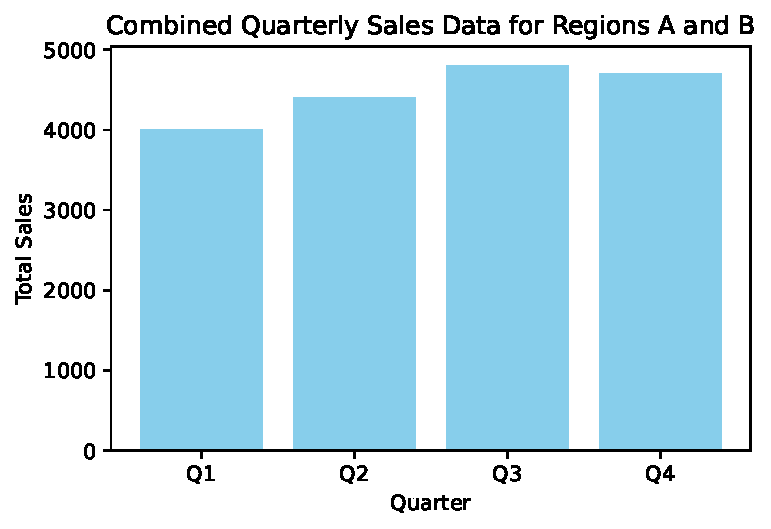
\includegraphics{module_2_files/figure-pdf/fig-total1-output-1.pdf}

}

\caption{\label{fig-total1}Computing Total Sales using \texttt{Numpy}
aggregation method}

\end{figure}%

In the above \texttt{Python} code, we have performed the aggregation
operation with the \texttt{NumPy} method. Same can be done in a more
data analysis style using \texttt{pandas} inorder to handle tabular data
meaningfully. In this approach, quarterly sales data of each region is
stored as \texttt{DataFrames}(like an excel sheet). The we combine these
two \texttt{DataFrames} into one. After that create a new row with index
`Total' and populate this row with sum of quarterly sales in Region A
and Region B. Finally a bar plot is created using this `Total' sales.
Advantage of this approach is that we don't need the \texttt{matplotlib}
library to create visualizations!. The EDA using this approach is shown
in Fig~\ref{fig-tot2}.

\begin{Shaded}
\begin{Highlighting}[]
\ImportTok{import}\NormalTok{ pandas }\ImportTok{as}\NormalTok{ pd}
\ImportTok{import}\NormalTok{ matplotlib.pyplot }\ImportTok{as}\NormalTok{ plt}

\CommentTok{\# DataFrames for quarterly sales data}
\NormalTok{df\_a }\OperatorTok{=}\NormalTok{ pd.DataFrame(\{}\StringTok{\textquotesingle{}Q1\textquotesingle{}}\NormalTok{: [}\DecValTok{2500}\NormalTok{], }\StringTok{\textquotesingle{}Q2\textquotesingle{}}\NormalTok{: [}\DecValTok{2800}\NormalTok{], }\StringTok{\textquotesingle{}Q3\textquotesingle{}}\NormalTok{: [}\DecValTok{3100}\NormalTok{], }\StringTok{\textquotesingle{}Q4\textquotesingle{}}\NormalTok{: [}\DecValTok{2900}\NormalTok{]\}, index}\OperatorTok{=}\NormalTok{[}\StringTok{\textquotesingle{}Region A\textquotesingle{}}\NormalTok{])}
\NormalTok{df\_b }\OperatorTok{=}\NormalTok{ pd.DataFrame(\{}\StringTok{\textquotesingle{}Q1\textquotesingle{}}\NormalTok{: [}\DecValTok{1500}\NormalTok{], }\StringTok{\textquotesingle{}Q2\textquotesingle{}}\NormalTok{: [}\DecValTok{1600}\NormalTok{], }\StringTok{\textquotesingle{}Q3\textquotesingle{}}\NormalTok{: [}\DecValTok{1700}\NormalTok{], }\StringTok{\textquotesingle{}Q4\textquotesingle{}}\NormalTok{: [}\DecValTok{1800}\NormalTok{]\}, index}\OperatorTok{=}\NormalTok{[}\StringTok{\textquotesingle{}Region B\textquotesingle{}}\NormalTok{])}

\CommentTok{\# Combine data}
\NormalTok{df\_combined }\OperatorTok{=}\NormalTok{ df\_a.add(df\_b, fill\_value}\OperatorTok{=}\DecValTok{0}\NormalTok{)}
\NormalTok{df\_combined.loc[}\StringTok{"Total"}\NormalTok{] }\OperatorTok{=}\NormalTok{ df\_combined.}\BuiltInTok{sum}\NormalTok{(axis}\OperatorTok{=}\DecValTok{0}\NormalTok{)}
\CommentTok{\# Visualization}
\NormalTok{df\_combined.loc[}\StringTok{"Total"}\NormalTok{].plot(kind}\OperatorTok{=}\StringTok{\textquotesingle{}bar\textquotesingle{}}\NormalTok{, color}\OperatorTok{=}\NormalTok{[}\StringTok{\textquotesingle{}green\textquotesingle{}}\NormalTok{])}
\NormalTok{plt.xlabel(}\StringTok{\textquotesingle{}Quarter\textquotesingle{}}\NormalTok{)}
\NormalTok{plt.ylabel(}\StringTok{\textquotesingle{}Total Sales\textquotesingle{}}\NormalTok{)}
\NormalTok{plt.title(}\StringTok{\textquotesingle{}Combined Quarterly Sales Data for Regions A and B\textquotesingle{}}\NormalTok{)}
\NormalTok{plt.show()}
\end{Highlighting}
\end{Shaded}

\begin{figure}[H]

\centering{

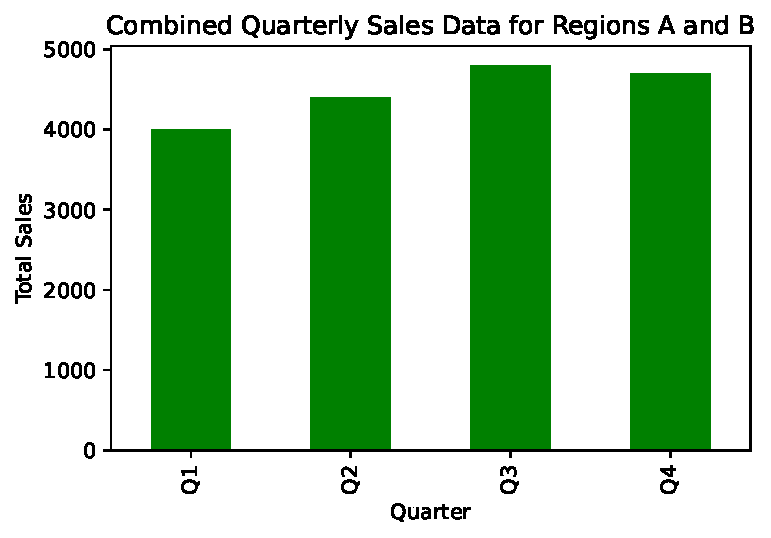
\includegraphics{module_2_files/figure-pdf/fig-tot2-output-1.pdf}

}

\caption{\label{fig-tot2}Computation of Total Sales using
\texttt{Pandas} method}

\end{figure}%

We can extend this in to more advanced examples. Irrespective to the
size of the data, for representation and aggregation tasks matrix models
are best options and are used in industry as a standard. Let us consider
an advanced example to analyse difference in stock prices. For this
example we are using a simulated data. The python code for this
simulation process is shown in Fig~\ref{fig-sim}.

\begin{Shaded}
\begin{Highlighting}[]
\ImportTok{import}\NormalTok{ numpy }\ImportTok{as}\NormalTok{ np}
\ImportTok{import}\NormalTok{ matplotlib.pyplot }\ImportTok{as}\NormalTok{ plt}

\CommentTok{\# Simulated observed and predicted stock prices}
\NormalTok{observed\_prices }\OperatorTok{=}\NormalTok{ np.random.uniform(}\DecValTok{100}\NormalTok{, }\DecValTok{200}\NormalTok{, size}\OperatorTok{=}\NormalTok{(}\DecValTok{100}\NormalTok{, }\DecValTok{5}\NormalTok{))}
\NormalTok{predicted\_prices }\OperatorTok{=}\NormalTok{ np.random.uniform(}\DecValTok{95}\NormalTok{, }\DecValTok{210}\NormalTok{, size}\OperatorTok{=}\NormalTok{(}\DecValTok{100}\NormalTok{, }\DecValTok{5}\NormalTok{))}

\CommentTok{\# Calculate the difference matrix}
\NormalTok{price\_differences }\OperatorTok{=}\NormalTok{ observed\_prices }\OperatorTok{{-}}\NormalTok{ predicted\_prices}

\CommentTok{\# Visualization}
\NormalTok{plt.imshow(price\_differences, cmap}\OperatorTok{=}\StringTok{\textquotesingle{}coolwarm\textquotesingle{}}\NormalTok{, aspect}\OperatorTok{=}\StringTok{\textquotesingle{}auto\textquotesingle{}}\NormalTok{)}
\NormalTok{plt.colorbar()}
\NormalTok{plt.title(}\StringTok{\textquotesingle{}Stock Price Differences\textquotesingle{}}\NormalTok{)}
\NormalTok{plt.xlabel(}\StringTok{\textquotesingle{}Stock Index\textquotesingle{}}\NormalTok{)}
\NormalTok{plt.ylabel(}\StringTok{\textquotesingle{}Day Index\textquotesingle{}}\NormalTok{)}
\NormalTok{plt.show()}
\end{Highlighting}
\end{Shaded}

\begin{figure}[H]

\centering{

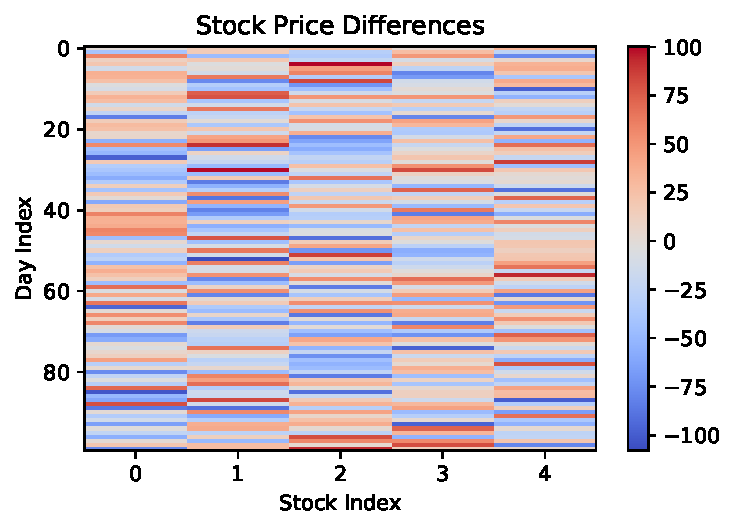
\includegraphics{module_2_files/figure-pdf/fig-sim-output-1.pdf}

}

\caption{\label{fig-sim}Demonstration of Stock Price simulated from a
Uniform Distribution}

\end{figure}%

Another important matrix operation relevant to data analytics and
Machine Learning application is scaling. This is considered as a
statistical tool to make various features (attributes) in to same scale
so as to avoid unnecessary misleading impact in data analysis and its
intepretation. In Machine Learning context, this pre-processing stage is
inevitable so as to make the model relevant and usable.

\textbf{Simple Example: Normalizing Employee Performance Data}

\begin{longtable}[]{@{}lll@{}}
\caption{Employee Performance Data}\label{tbl-EPD}\tabularnewline
\toprule\noalign{}
Employee & Metric A & Metric B \\
\midrule\noalign{}
\endfirsthead
\toprule\noalign{}
Employee & Metric A & Metric B \\
\midrule\noalign{}
\endhead
\bottomrule\noalign{}
\endlastfoot
X & 80 & 700 \\
Y & 90 & 800 \\
Z & 100 & 900 \\
A & 110 & 1000 \\
B & 120 & 1100 \\
\end{longtable}

Using simple python code we can simulate the model for \texttt{min-max}
scaling. The formula for \texttt{min-max} scaling is:
\[min_max(X)=\dfrac{X-min(X)}{max(X)-min(X)}\]

For example, while applying the \texttt{min-max} scaling in the first
value of Metric A, the scaled value is
\[min_max(80)\dfrac{80-80}{120-80}=0\]

Similarly

\[min_max(100)\dfrac{100-80}{120-80}=0.5\]

When we apply this formula to Metric A and Metric B, the scaled output
from Table~\ref{tbl-EPD} will be as follows:

\begin{longtable}[]{@{}lll@{}}
\caption{Employee Performance Data}\label{tbl-EPDu}\tabularnewline
\toprule\noalign{}
Employee & Metric A & Metric B \\
\midrule\noalign{}
\endfirsthead
\toprule\noalign{}
Employee & Metric A & Metric B \\
\midrule\noalign{}
\endhead
\bottomrule\noalign{}
\endlastfoot
X & 0.00 & 0.00 \\
Y & 0.25 & 0.25 \\
Z & 0.50 & 0.50 \\
A & 0.75 & 0.75 \\
B & 1.00 & 1.00 \\
\end{longtable}

It is interesting to look into the scaled data! In the orginal table
(Table~\ref{tbl-EPD}) it is looked like Metric B is superior. But from
the scaled table (Table~\ref{tbl-EPDu}), it is clear that both the
Metrics are representing same relative information. This will help us to
identify the redundency in measure and so skip any one of the Metric
before analysis!.

The same can be achieved through a matrix operation. The \texttt{Python}
implementation of this scaling process is shown in
Fig~\ref{fig-totalsales}.

\begin{Shaded}
\begin{Highlighting}[]
\ImportTok{import}\NormalTok{ numpy }\ImportTok{as}\NormalTok{ np}
\ImportTok{import}\NormalTok{ matplotlib.pyplot }\ImportTok{as}\NormalTok{ plt}

\CommentTok{\# Employee performance data with varying scales}
\NormalTok{data }\OperatorTok{=}\NormalTok{ np.array([[}\DecValTok{80}\NormalTok{, }\DecValTok{700}\NormalTok{], [}\DecValTok{90}\NormalTok{, }\DecValTok{800}\NormalTok{], [}\DecValTok{100}\NormalTok{, }\DecValTok{900}\NormalTok{], [}\DecValTok{110}\NormalTok{, }\DecValTok{1000}\NormalTok{], [}\DecValTok{120}\NormalTok{, }\DecValTok{1100}\NormalTok{]])}

\CommentTok{\# Manual scaling}
\NormalTok{min\_vals }\OperatorTok{=}\NormalTok{ np.}\BuiltInTok{min}\NormalTok{(data, axis}\OperatorTok{=}\DecValTok{0}\NormalTok{)}
\NormalTok{max\_vals }\OperatorTok{=}\NormalTok{ np.}\BuiltInTok{max}\NormalTok{(data, axis}\OperatorTok{=}\DecValTok{0}\NormalTok{)}
\NormalTok{scaled\_data }\OperatorTok{=}\NormalTok{ (data }\OperatorTok{{-}}\NormalTok{ min\_vals) }\OperatorTok{/}\NormalTok{ (max\_vals }\OperatorTok{{-}}\NormalTok{ min\_vals)}

\CommentTok{\# Visualization}
\NormalTok{plt.figure(figsize}\OperatorTok{=}\NormalTok{(}\DecValTok{8}\NormalTok{, }\DecValTok{5}\NormalTok{))}
\NormalTok{plt.subplot(}\DecValTok{1}\NormalTok{, }\DecValTok{2}\NormalTok{, }\DecValTok{1}\NormalTok{)}
\NormalTok{plt.imshow(data, cmap}\OperatorTok{=}\StringTok{\textquotesingle{}viridis\textquotesingle{}}\NormalTok{)}
\NormalTok{plt.title(}\StringTok{\textquotesingle{}Original Data\textquotesingle{}}\NormalTok{)}
\NormalTok{plt.colorbar()}

\NormalTok{plt.subplot(}\DecValTok{1}\NormalTok{, }\DecValTok{2}\NormalTok{, }\DecValTok{2}\NormalTok{)}
\NormalTok{plt.imshow(scaled\_data, cmap}\OperatorTok{=}\StringTok{\textquotesingle{}viridis\textquotesingle{}}\NormalTok{)}
\NormalTok{plt.title(}\StringTok{\textquotesingle{}Scaled Data\textquotesingle{}}\NormalTok{)}
\NormalTok{plt.colorbar()}

\NormalTok{plt.show()}
\end{Highlighting}
\end{Shaded}

\begin{figure}[H]

\centering{

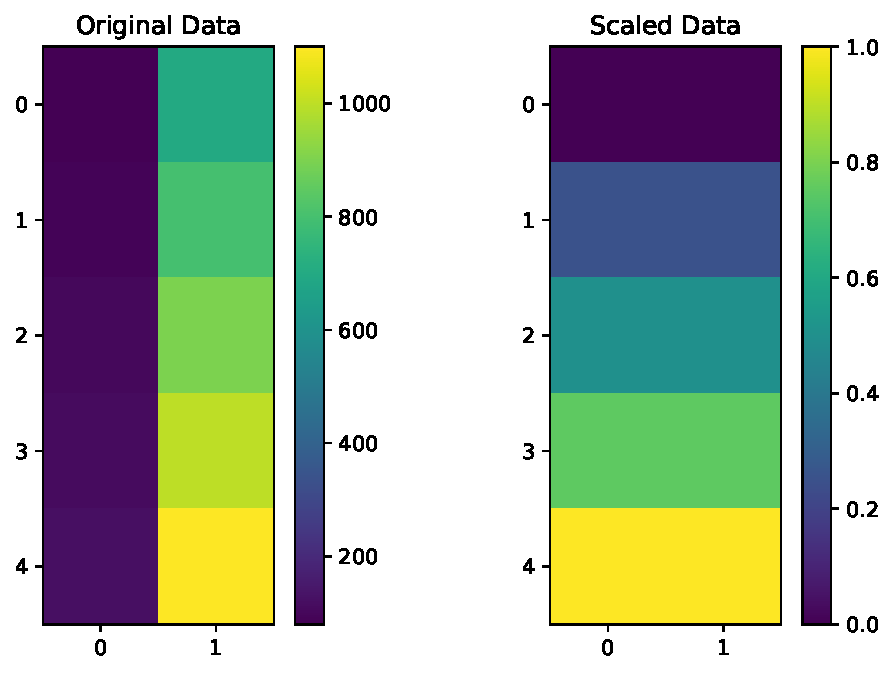
\includegraphics{module_2_files/figure-pdf/fig-totalsales-output-1.pdf}

}

\caption{\label{fig-totalsales}Total sales using \texttt{pandas} method}

\end{figure}%

From the first sub plot, it is clear that there is a significant
difference in the distributions (Metric A and Metric B values). But the
second sub plot shows that both the distributions have same pattern and
the values ranges between 0 and 1. In short the visualization is more
appealing and self explanatory in this case.

\begin{tcolorbox}[enhanced jigsaw, leftrule=.75mm, bottomtitle=1mm, colback=white, toptitle=1mm, opacitybacktitle=0.6, toprule=.15mm, colbacktitle=quarto-callout-note-color!10!white, arc=.35mm, colframe=quarto-callout-note-color-frame, title=\textcolor{quarto-callout-note-color}{\faInfo}\hspace{0.5em}{Note}, titlerule=0mm, rightrule=.15mm, left=2mm, bottomrule=.15mm, breakable, coltitle=black, opacityback=0]

The \texttt{min-max} scaling method will confine the feature values
(attributes) into the range \([0,1]\). So in effect all the features are
scaled proportionally to the data spectrum.

\end{tcolorbox}

Similarly, we can use the \texttt{standard\ scaling} (transformation to
normal distribution) using the transformation
\(\dfrac{x-\bar{x}}{\sigma}\). Scaling table is given as a practice task
to the reader. The python code for this operation is shown in
Fig~\ref{fig-minmax}.

\begin{Shaded}
\begin{Highlighting}[]
\CommentTok{\# Standard scaling from scratch}
\KeywordTok{def}\NormalTok{ standard\_scaling(data):}
\NormalTok{    mean }\OperatorTok{=}\NormalTok{ np.mean(data, axis}\OperatorTok{=}\DecValTok{0}\NormalTok{)}
\NormalTok{    std }\OperatorTok{=}\NormalTok{ np.std(data, axis}\OperatorTok{=}\DecValTok{0}\NormalTok{)}
\NormalTok{    scaled\_data }\OperatorTok{=}\NormalTok{ (data }\OperatorTok{{-}}\NormalTok{ mean) }\OperatorTok{/}\NormalTok{ std}
    \ControlFlowTok{return}\NormalTok{ scaled\_data}

\CommentTok{\# Apply standard scaling}
\NormalTok{scaled\_data\_scratch }\OperatorTok{=}\NormalTok{ standard\_scaling(data)}

\BuiltInTok{print}\NormalTok{(}\StringTok{"Standard Scaled Data (from scratch):}\CharTok{\textbackslash{}n}\StringTok{"}\NormalTok{, scaled\_data\_scratch)}

\CommentTok{\# Visualization}
\NormalTok{plt.figure(figsize}\OperatorTok{=}\NormalTok{(}\DecValTok{6}\NormalTok{, }\DecValTok{5}\NormalTok{))}
\NormalTok{plt.subplot(}\DecValTok{1}\NormalTok{, }\DecValTok{2}\NormalTok{, }\DecValTok{1}\NormalTok{)}
\NormalTok{plt.imshow(data, cmap}\OperatorTok{=}\StringTok{\textquotesingle{}viridis\textquotesingle{}}\NormalTok{)}
\NormalTok{plt.title(}\StringTok{\textquotesingle{}Original Data\textquotesingle{}}\NormalTok{)}
\NormalTok{plt.colorbar()}

\NormalTok{plt.subplot(}\DecValTok{1}\NormalTok{, }\DecValTok{2}\NormalTok{, }\DecValTok{2}\NormalTok{)}
\NormalTok{plt.imshow(scaled\_data\_scratch, cmap}\OperatorTok{=}\StringTok{\textquotesingle{}viridis\textquotesingle{}}\NormalTok{)}
\NormalTok{plt.title(}\StringTok{\textquotesingle{}Scaled Data\textquotesingle{}}\NormalTok{)}
\NormalTok{plt.colorbar()}

\NormalTok{plt.show()}
\end{Highlighting}
\end{Shaded}

\begin{verbatim}
Standard Scaled Data (from scratch):
 [[-1.41421356 -1.41421356]
 [-0.70710678 -0.70710678]
 [ 0.          0.        ]
 [ 0.70710678  0.70710678]
 [ 1.41421356  1.41421356]]
\end{verbatim}

\begin{figure}[H]

\centering{

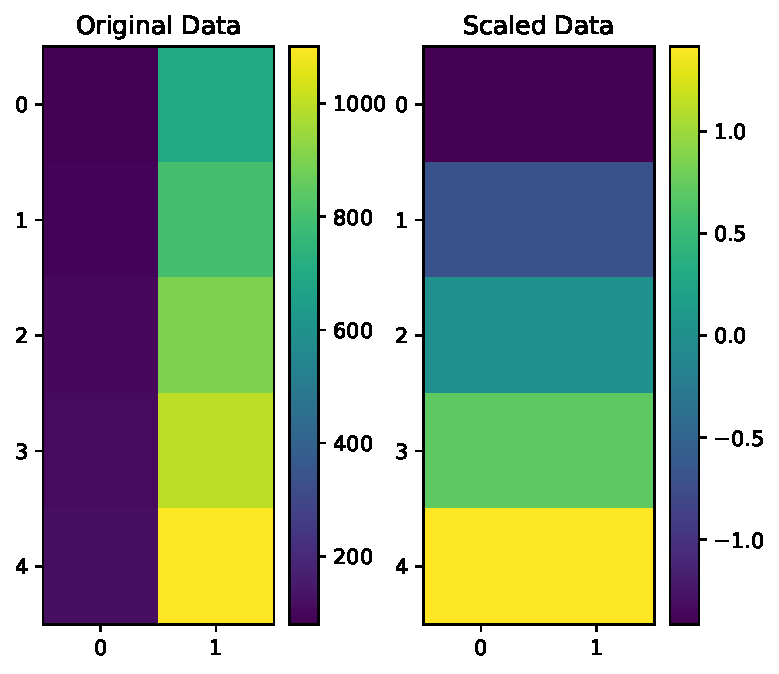
\includegraphics{module_2_files/figure-pdf/fig-minmax-output-2.pdf}

}

\caption{\label{fig-minmax}Min-max scaling using basic python}

\end{figure}%

To understand the effect of standard scaling, let us consider
Fig~\ref{fig-comp1}. This plot create the frequency distribution of the
data as a histogram along with the density function. From the first
sub-plot, it is clear that the distribution has multiple modes (peaks).
When we apply the standard scaling, the distribution become
un-modal(only one peek). This is demonstrated in the second sub-plot.

\begin{Shaded}
\begin{Highlighting}[]
\CommentTok{\# Standard scaling from scratch}
\ImportTok{import}\NormalTok{ seaborn }\ImportTok{as}\NormalTok{ sns}
\CommentTok{\# Create plots}
\NormalTok{plt.figure(figsize}\OperatorTok{=}\NormalTok{(}\DecValTok{6}\NormalTok{, }\DecValTok{5}\NormalTok{))}

\CommentTok{\# Plot for original data}
\NormalTok{plt.subplot(}\DecValTok{1}\NormalTok{, }\DecValTok{2}\NormalTok{, }\DecValTok{1}\NormalTok{)}
\NormalTok{sns.histplot(data, kde}\OperatorTok{=}\VariableTok{True}\NormalTok{, bins}\OperatorTok{=}\DecValTok{10}\NormalTok{, palette}\OperatorTok{=}\StringTok{"viridis"}\NormalTok{)}
\NormalTok{plt.title(}\StringTok{\textquotesingle{}Original Data Distribution\textquotesingle{}}\NormalTok{)}
\NormalTok{plt.xlabel(}\StringTok{\textquotesingle{}Value\textquotesingle{}}\NormalTok{)}
\NormalTok{plt.ylabel(}\StringTok{\textquotesingle{}Frequency\textquotesingle{}}\NormalTok{)}

\CommentTok{\# Plot for standard scaled data}
\NormalTok{plt.subplot(}\DecValTok{1}\NormalTok{, }\DecValTok{2}\NormalTok{, }\DecValTok{2}\NormalTok{)}
\NormalTok{sns.histplot(scaled\_data\_scratch, kde}\OperatorTok{=}\VariableTok{True}\NormalTok{, bins}\OperatorTok{=}\DecValTok{10}\NormalTok{, palette}\OperatorTok{=}\StringTok{"viridis"}\NormalTok{)}
\NormalTok{plt.title(}\StringTok{\textquotesingle{}Standard Scaled Data Distribution\textquotesingle{}}\NormalTok{)}
\NormalTok{plt.xlabel(}\StringTok{\textquotesingle{}Value\textquotesingle{}}\NormalTok{)}
\NormalTok{plt.ylabel(}\StringTok{\textquotesingle{}Frequency\textquotesingle{}}\NormalTok{)}

\NormalTok{plt.tight\_layout()}
\NormalTok{plt.show()}
\end{Highlighting}
\end{Shaded}

\begin{figure}[H]

\centering{

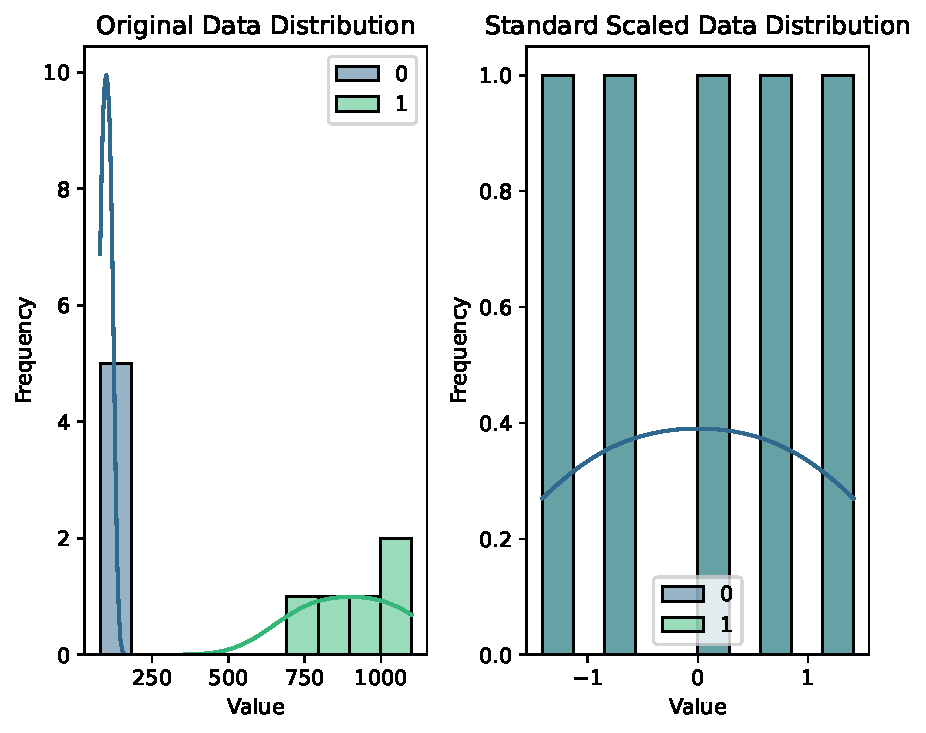
\includegraphics{module_2_files/figure-pdf/fig-comp1-output-1.pdf}

}

\caption{\label{fig-comp1}Impact of standard scaling on the
distribution}

\end{figure}%

A scatter plot showing the compare the impact of scaling on the given
distribution is shown in Fig~\ref{fig-scatter}.

\begin{Shaded}
\begin{Highlighting}[]
\CommentTok{\# Plot original and scaled data}
\NormalTok{plt.figure(figsize}\OperatorTok{=}\NormalTok{(}\DecValTok{6}\NormalTok{, }\DecValTok{5}\NormalTok{))}

\CommentTok{\# Original Data}
\NormalTok{plt.subplot(}\DecValTok{1}\NormalTok{, }\DecValTok{3}\NormalTok{, }\DecValTok{1}\NormalTok{)}
\NormalTok{plt.scatter(data[:, }\DecValTok{0}\NormalTok{], data[:, }\DecValTok{1}\NormalTok{], color}\OperatorTok{=}\StringTok{\textquotesingle{}blue\textquotesingle{}}\NormalTok{)}
\NormalTok{plt.title(}\StringTok{\textquotesingle{}Original Data\textquotesingle{}}\NormalTok{)}
\NormalTok{plt.xlabel(}\StringTok{\textquotesingle{}Metric A\textquotesingle{}}\NormalTok{)}
\NormalTok{plt.ylabel(}\StringTok{\textquotesingle{}Metric B\textquotesingle{}}\NormalTok{)}

\CommentTok{\# Standard Scaled Data}
\NormalTok{plt.subplot(}\DecValTok{1}\NormalTok{, }\DecValTok{3}\NormalTok{, }\DecValTok{2}\NormalTok{)}
\NormalTok{plt.scatter(scaled\_data\_scratch[:, }\DecValTok{0}\NormalTok{], scaled\_data\_scratch[:, }\DecValTok{1}\NormalTok{], color}\OperatorTok{=}\StringTok{\textquotesingle{}green\textquotesingle{}}\NormalTok{)}
\NormalTok{plt.title(}\StringTok{\textquotesingle{}Standard Scaled Data\textquotesingle{}}\NormalTok{)}
\NormalTok{plt.xlabel(}\StringTok{\textquotesingle{}Metric A (Standard Scaled)\textquotesingle{}}\NormalTok{)}
\NormalTok{plt.ylabel(}\StringTok{\textquotesingle{}Metric B (Standard Scaled)\textquotesingle{}}\NormalTok{)}

\CommentTok{\# Min{-}Max Scaled Data}
\NormalTok{plt.subplot(}\DecValTok{1}\NormalTok{, }\DecValTok{3}\NormalTok{, }\DecValTok{3}\NormalTok{)}
\NormalTok{plt.scatter(scaled\_data[:, }\DecValTok{0}\NormalTok{], scaled\_data[:, }\DecValTok{1}\NormalTok{], color}\OperatorTok{=}\StringTok{\textquotesingle{}red\textquotesingle{}}\NormalTok{)}
\NormalTok{plt.title(}\StringTok{\textquotesingle{}Min{-}Max Scaled Data\textquotesingle{}}\NormalTok{)}
\NormalTok{plt.xlabel(}\StringTok{\textquotesingle{}Metric A (Min{-}Max Scaled)\textquotesingle{}}\NormalTok{)}
\NormalTok{plt.ylabel(}\StringTok{\textquotesingle{}Metric B (Min{-}Max Scaled)\textquotesingle{}}\NormalTok{)}

\NormalTok{plt.tight\_layout()}
\NormalTok{plt.show()}
\end{Highlighting}
\end{Shaded}

\begin{figure}[H]

\centering{

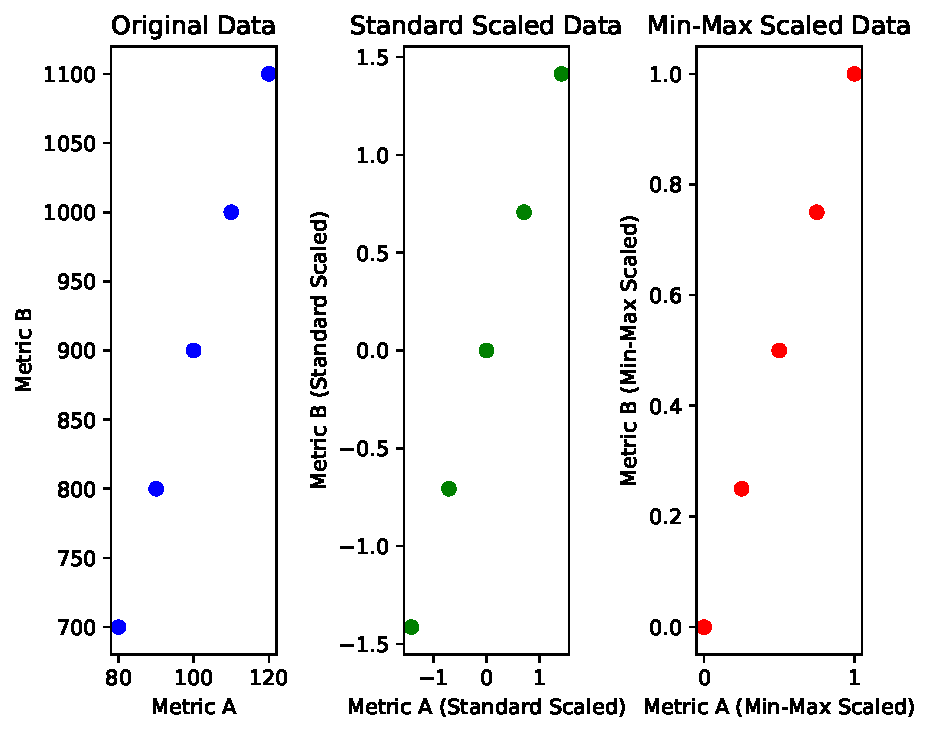
\includegraphics{module_2_files/figure-pdf/fig-scatter-output-1.pdf}

}

\caption{\label{fig-scatter}Comparison of impact of scaling on the
distribution}

\end{figure}%

From the Fig~\ref{fig-scatter}, it is clear that the scaling does not
affect the pattern of the data, instead it just scale the distribution
proportionally!

We can use the \texttt{scikit-learn} library for do the same thing in a
very simple handy approach. The \texttt{python} code for this job is
shown below.

\begin{Shaded}
\begin{Highlighting}[]
\ImportTok{from}\NormalTok{ sklearn.preprocessing }\ImportTok{import}\NormalTok{ MinMaxScaler}

\CommentTok{\# Min{-}max scaling using sklearn}
\NormalTok{scaler }\OperatorTok{=}\NormalTok{ MinMaxScaler()}
\NormalTok{min\_max\_scaled\_data\_sklearn }\OperatorTok{=}\NormalTok{ scaler.fit\_transform(data)}

\BuiltInTok{print}\NormalTok{(}\StringTok{"Min{-}Max Scaled Data (using sklearn):}\CharTok{\textbackslash{}n}\StringTok{"}\NormalTok{, min\_max\_scaled\_data\_sklearn)}
\end{Highlighting}
\end{Shaded}

\begin{verbatim}
Min-Max Scaled Data (using sklearn):
 [[0.   0.  ]
 [0.25 0.25]
 [0.5  0.5 ]
 [0.75 0.75]
 [1.   1.  ]]
\end{verbatim}

\begin{Shaded}
\begin{Highlighting}[]
\ImportTok{from}\NormalTok{ sklearn.preprocessing }\ImportTok{import}\NormalTok{ StandardScaler}

\CommentTok{\# Standard scaling using sklearn}
\NormalTok{scaler }\OperatorTok{=}\NormalTok{ StandardScaler()}
\NormalTok{scaled\_data\_sklearn }\OperatorTok{=}\NormalTok{ scaler.fit\_transform(data)}

\BuiltInTok{print}\NormalTok{(}\StringTok{"Standard Scaled Data (using sklearn):}\CharTok{\textbackslash{}n}\StringTok{"}\NormalTok{, scaled\_data\_sklearn)}
\end{Highlighting}
\end{Shaded}

\begin{verbatim}
Standard Scaled Data (using sklearn):
 [[-1.41421356 -1.41421356]
 [-0.70710678 -0.70710678]
 [ 0.          0.        ]
 [ 0.70710678  0.70710678]
 [ 1.41421356  1.41421356]]
\end{verbatim}

A scatter plot showing the impact on scaling is shown in
Fig~\ref{fig-comp2}. This plot compare the m\texttt{min-max} and
\texttt{standard-scaling}.

\begin{Shaded}
\begin{Highlighting}[]
\CommentTok{\# Plot original and scaled data}
\NormalTok{plt.figure(figsize}\OperatorTok{=}\NormalTok{(}\DecValTok{6}\NormalTok{, }\DecValTok{5}\NormalTok{))}

\CommentTok{\# Original Data}
\NormalTok{plt.subplot(}\DecValTok{1}\NormalTok{, }\DecValTok{3}\NormalTok{, }\DecValTok{1}\NormalTok{)}
\NormalTok{plt.scatter(data[:, }\DecValTok{0}\NormalTok{], data[:, }\DecValTok{1}\NormalTok{], color}\OperatorTok{=}\StringTok{\textquotesingle{}blue\textquotesingle{}}\NormalTok{)}
\NormalTok{plt.title(}\StringTok{\textquotesingle{}Original Data\textquotesingle{}}\NormalTok{)}
\NormalTok{plt.xlabel(}\StringTok{\textquotesingle{}Metric A\textquotesingle{}}\NormalTok{)}
\NormalTok{plt.ylabel(}\StringTok{\textquotesingle{}Metric B\textquotesingle{}}\NormalTok{)}

\CommentTok{\# Standard Scaled Data}
\NormalTok{plt.subplot(}\DecValTok{1}\NormalTok{, }\DecValTok{3}\NormalTok{, }\DecValTok{2}\NormalTok{)}
\NormalTok{plt.scatter(scaled\_data\_sklearn[:, }\DecValTok{0}\NormalTok{], scaled\_data\_sklearn[:, }\DecValTok{1}\NormalTok{], color}\OperatorTok{=}\StringTok{\textquotesingle{}green\textquotesingle{}}\NormalTok{)}
\NormalTok{plt.title(}\StringTok{\textquotesingle{}Standard Scaled Data\textquotesingle{}}\NormalTok{)}
\NormalTok{plt.xlabel(}\StringTok{\textquotesingle{}Metric A (Standard Scaled)\textquotesingle{}}\NormalTok{)}
\NormalTok{plt.ylabel(}\StringTok{\textquotesingle{}Metric B (Standard Scaled)\textquotesingle{}}\NormalTok{)}

\CommentTok{\# Min{-}Max Scaled Data}
\NormalTok{plt.subplot(}\DecValTok{1}\NormalTok{, }\DecValTok{3}\NormalTok{, }\DecValTok{3}\NormalTok{)}
\NormalTok{plt.scatter(min\_max\_scaled\_data\_sklearn[:, }\DecValTok{0}\NormalTok{], min\_max\_scaled\_data\_sklearn[:, }\DecValTok{1}\NormalTok{], color}\OperatorTok{=}\StringTok{\textquotesingle{}red\textquotesingle{}}\NormalTok{)}
\NormalTok{plt.title(}\StringTok{\textquotesingle{}Min{-}Max Scaled Data\textquotesingle{}}\NormalTok{)}
\NormalTok{plt.xlabel(}\StringTok{\textquotesingle{}Metric A (Min{-}Max Scaled)\textquotesingle{}}\NormalTok{)}
\NormalTok{plt.ylabel(}\StringTok{\textquotesingle{}Metric B (Min{-}Max Scaled)\textquotesingle{}}\NormalTok{)}

\NormalTok{plt.tight\_layout()}
\NormalTok{plt.show()}
\end{Highlighting}
\end{Shaded}

\begin{figure}[H]

\centering{

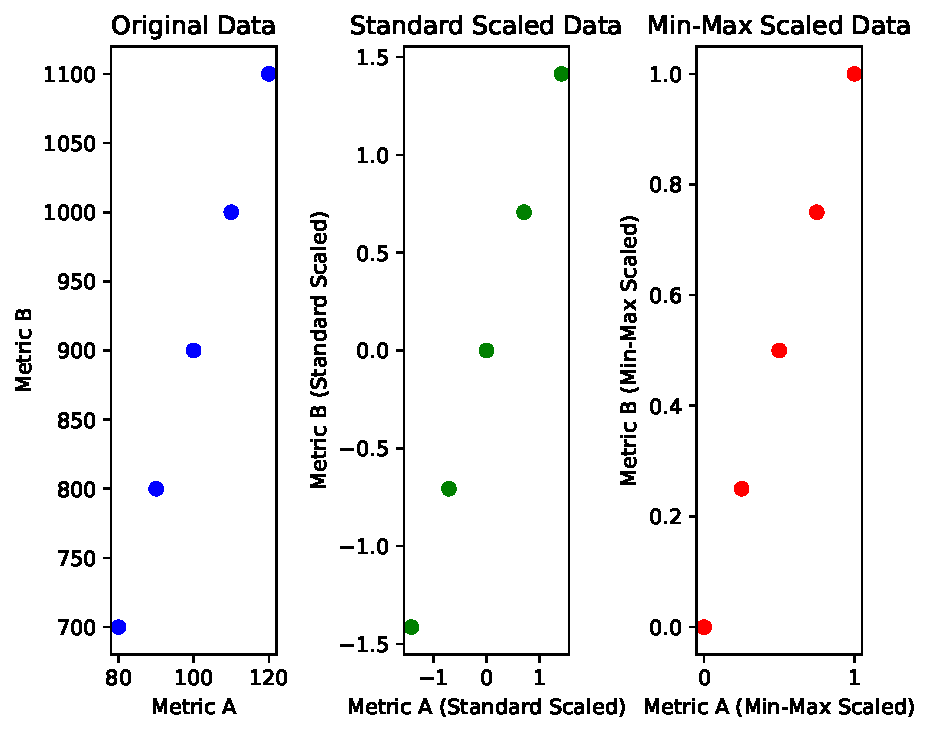
\includegraphics{module_2_files/figure-pdf/fig-comp2-output-1.pdf}

}

\caption{\label{fig-comp2}Camparison of Min-max and standard scalings
with original data}

\end{figure}%

\subsection*{More on Matrix Product and its
Applications}\label{more-on-matrix-product-and-its-applications}
\addcontentsline{toc}{subsection}{More on Matrix Product and its
Applications}

In the first module of our course, we introduced matrix products as
scalar projections, focusing on how matrices interact through basic
operations. In this section, we will expand on this by exploring
different types of matrix products that have practical importance in
various fields. One such product is the \emph{Hadamard product}, which
is particularly useful in applications ranging from image processing to
neural networks and statistical analysis. We will cover the definition,
properties, and examples of the Hadamard product, and then delve into
practical applications with simulated data.

\subsubsection*{Hadamard Product}\label{hadamard-product}
\addcontentsline{toc}{subsubsection}{Hadamard Product}

The Hadamard product (or element-wise product) of two matrices is a
binary operation that combines two matrices of the same dimensions to
produce another matrix of the same dimensions, where each element is the
product of corresponding elements in the original matrices.

\begin{tcolorbox}[enhanced jigsaw, leftrule=.75mm, bottomtitle=1mm, colback=white, toptitle=1mm, opacitybacktitle=0.6, toprule=.15mm, colbacktitle=quarto-callout-important-color!10!white, arc=.35mm, colframe=quarto-callout-important-color-frame, title=\textcolor{quarto-callout-important-color}{\faExclamation}\hspace{0.5em}{Definition (Hadamard Product):}, titlerule=0mm, rightrule=.15mm, left=2mm, bottomrule=.15mm, breakable, coltitle=black, opacityback=0]

For two matrices \(A\) and \(B\) of the same dimension \(m \times n\),
the Hadamard product \(A \circ B\) is defined as:

\[(A \circ B)_{ij} = A_{ij} \cdot B_{ij}\]

where \(\cdot\) denotes element-wise multiplication.

\end{tcolorbox}

\begin{tcolorbox}[enhanced jigsaw, leftrule=.75mm, bottomtitle=1mm, colback=white, toptitle=1mm, opacitybacktitle=0.6, toprule=.15mm, colbacktitle=quarto-callout-note-color!10!white, arc=.35mm, colframe=quarto-callout-note-color-frame, title=\textcolor{quarto-callout-note-color}{\faInfo}\hspace{0.5em}{Properties of Hadamard Product}, titlerule=0mm, rightrule=.15mm, left=2mm, bottomrule=.15mm, breakable, coltitle=black, opacityback=0]

\begin{enumerate}
\def\labelenumi{\arabic{enumi}.}
\item
  \textbf{Commutativity}: \[A \circ B = B \circ A\]
\item
  \textbf{Associativity}: \[(A \circ B) \circ C = A \circ (B \circ C)\]
\item
  \textbf{Distributivity}:
  \[A \circ (B + C) = (A \circ B) + (A \circ C)\]
\end{enumerate}

\end{tcolorbox}

Some simple examples to demonstrate the Hadamard product is given below.

Example 1: Basic Hadamard Product

Given matrices:

\[A = \begin{pmatrix}1 & 2 \\3 & 4\end{pmatrix}, \quad B = \begin{pmatrix}5 & 6 \\7 & 8\end{pmatrix}\]

The Hadamard product \(A \circ B\) is:

\[A \circ B = \begin{pmatrix}1 \cdot 5 & 2 \cdot 6 \\3 \cdot 7 & 4 \cdot 8\end{pmatrix} = \begin{pmatrix}5 & 12 \\21 & 32\end{pmatrix}\]

Example 2: Hadamard Product with Larger Matrices

Given matrices:

\[A = \begin{pmatrix}1 & 2 & 3 \\4 & 5 & 6 \\7 & 8 & 9\end{pmatrix}, \quad B = \begin{pmatrix}9 & 8 & 7 \\6 & 5 & 4 \\3 & 2 & 1\end{pmatrix}\]

The Hadamard product \(A \circ B\) is:

\[A \circ B = \begin{pmatrix}1 \cdot 9 & 2 \cdot 8 & 3 \cdot 7 \\4 \cdot 6 & 5 \cdot 5 & 6 \cdot 4 \\7 \cdot 3 & 8 \cdot  & 9 \cdot 1\end{pmatrix} = \begin{pmatrix}9 & 16 & 21 \\24 & 25 & 24 \\21 & 16 & 9\end{pmatrix}\]

In the following code chunks the computational process of Hadamard
product is implemented in \texttt{Python}. Here both the from the
scratch and use of external module versions are included.

\textbf{1. Compute Hadamard Product from Scratch (without Libraries)}

Here's how you can compute the Hadamard product manually:

\begin{Shaded}
\begin{Highlighting}[]
\CommentTok{\# Define matrices A and B}
\NormalTok{A }\OperatorTok{=}\NormalTok{ [[}\DecValTok{1}\NormalTok{, }\DecValTok{2}\NormalTok{, }\DecValTok{3}\NormalTok{], [}\DecValTok{4}\NormalTok{, }\DecValTok{5}\NormalTok{, }\DecValTok{6}\NormalTok{]]}
\NormalTok{B }\OperatorTok{=}\NormalTok{ [[}\DecValTok{7}\NormalTok{, }\DecValTok{8}\NormalTok{, }\DecValTok{9}\NormalTok{], [}\DecValTok{10}\NormalTok{, }\DecValTok{11}\NormalTok{, }\DecValTok{12}\NormalTok{]]}

\CommentTok{\# Function to compute Hadamard product}
\KeywordTok{def}\NormalTok{ hadamard\_product(A, B):}
    \CommentTok{\# Get the number of rows and columns}
\NormalTok{    num\_rows }\OperatorTok{=} \BuiltInTok{len}\NormalTok{(A)}
\NormalTok{    num\_cols }\OperatorTok{=} \BuiltInTok{len}\NormalTok{(A[}\DecValTok{0}\NormalTok{])}
    
    \CommentTok{\# Initialize the result matrix}
\NormalTok{    result }\OperatorTok{=}\NormalTok{ [[}\DecValTok{0}\NormalTok{]}\OperatorTok{*}\NormalTok{num\_cols }\ControlFlowTok{for}\NormalTok{ \_ }\KeywordTok{in} \BuiltInTok{range}\NormalTok{(num\_rows)]}
    
    \CommentTok{\# Compute the Hadamard product}
    \ControlFlowTok{for}\NormalTok{ i }\KeywordTok{in} \BuiltInTok{range}\NormalTok{(num\_rows):}
        \ControlFlowTok{for}\NormalTok{ j }\KeywordTok{in} \BuiltInTok{range}\NormalTok{(num\_cols):}
\NormalTok{            result[i][j] }\OperatorTok{=}\NormalTok{ A[i][j] }\OperatorTok{*}\NormalTok{ B[i][j]}
    
    \ControlFlowTok{return}\NormalTok{ result}

\CommentTok{\# Compute Hadamard product}
\NormalTok{hadamard\_product\_result }\OperatorTok{=}\NormalTok{ hadamard\_product(A, B)}

\CommentTok{\# Display result}
\BuiltInTok{print}\NormalTok{(}\StringTok{"Hadamard Product (From Scratch):"}\NormalTok{)}
\ControlFlowTok{for}\NormalTok{ row }\KeywordTok{in}\NormalTok{ hadamard\_product\_result:}
    \BuiltInTok{print}\NormalTok{(row)}
\end{Highlighting}
\end{Shaded}

\begin{verbatim}
Hadamard Product (From Scratch):
[7, 16, 27]
[40, 55, 72]
\end{verbatim}

\textbf{2. Compute Hadamard Product Using \texttt{SymPy}}

Here's how to compute the Hadamard product using \texttt{SymPy}:

\begin{Shaded}
\begin{Highlighting}[]
\ImportTok{import}\NormalTok{ sympy }\ImportTok{as}\NormalTok{ sp}

\CommentTok{\# Define matrices A and B}
\NormalTok{A }\OperatorTok{=}\NormalTok{ sp.Matrix([[}\DecValTok{1}\NormalTok{, }\DecValTok{2}\NormalTok{, }\DecValTok{3}\NormalTok{], [}\DecValTok{4}\NormalTok{, }\DecValTok{5}\NormalTok{, }\DecValTok{6}\NormalTok{]])}
\NormalTok{B }\OperatorTok{=}\NormalTok{ sp.Matrix([[}\DecValTok{7}\NormalTok{, }\DecValTok{8}\NormalTok{, }\DecValTok{9}\NormalTok{], [}\DecValTok{10}\NormalTok{, }\DecValTok{11}\NormalTok{, }\DecValTok{12}\NormalTok{]])}

\CommentTok{\# Compute Hadamard product using SymPy}
\NormalTok{Hadamard\_product\_sympy }\OperatorTok{=}\NormalTok{ A.multiply\_elementwise(B)}

\CommentTok{\# Display result}
\BuiltInTok{print}\NormalTok{(}\StringTok{"Hadamard Product (Using SymPy):"}\NormalTok{)}
\BuiltInTok{print}\NormalTok{(Hadamard\_product\_sympy)}
\end{Highlighting}
\end{Shaded}

\begin{verbatim}
Hadamard Product (Using SymPy):
Matrix([[7, 16, 27], [40, 55, 72]])
\end{verbatim}

\textbf{Practical Applications}

\emph{Application 1: Image Masking}

The Hadamard product can be used for image masking. Here's how you can
apply a mask to an image and visualize it as shown in
Fig~\ref{fig-imgmask}.

\begin{Shaded}
\begin{Highlighting}[]
\ImportTok{import}\NormalTok{ matplotlib.pyplot }\ImportTok{as}\NormalTok{ plt}
\ImportTok{import}\NormalTok{ numpy }\ImportTok{as}\NormalTok{ np}

\CommentTok{\# Simulated large image (2D array) using NumPy}
\NormalTok{image }\OperatorTok{=}\NormalTok{ np.random.rand(}\DecValTok{100}\NormalTok{, }\DecValTok{100}\NormalTok{)}

\CommentTok{\# Simulated mask (binary matrix) using NumPy}
\NormalTok{mask }\OperatorTok{=}\NormalTok{ np.random.randint(}\DecValTok{0}\NormalTok{, }\DecValTok{2}\NormalTok{, size}\OperatorTok{=}\NormalTok{(}\DecValTok{100}\NormalTok{, }\DecValTok{100}\NormalTok{))}

\CommentTok{\# Compute Hadamard product}
\NormalTok{masked\_image }\OperatorTok{=}\NormalTok{ image }\OperatorTok{*}\NormalTok{ mask}

\CommentTok{\# Plot original image and masked image}
\NormalTok{fig, ax }\OperatorTok{=}\NormalTok{ plt.subplots(}\DecValTok{1}\NormalTok{, }\DecValTok{2}\NormalTok{, figsize}\OperatorTok{=}\NormalTok{(}\DecValTok{12}\NormalTok{, }\DecValTok{5}\NormalTok{))}
\NormalTok{ax[}\DecValTok{0}\NormalTok{].imshow(image, cmap}\OperatorTok{=}\StringTok{\textquotesingle{}gray\textquotesingle{}}\NormalTok{)}
\NormalTok{ax[}\DecValTok{0}\NormalTok{].set\_title(}\StringTok{\textquotesingle{}Original Image\textquotesingle{}}\NormalTok{)}
\NormalTok{ax[}\DecValTok{1}\NormalTok{].imshow(masked\_image, cmap}\OperatorTok{=}\StringTok{\textquotesingle{}gray\textquotesingle{}}\NormalTok{)}
\NormalTok{ax[}\DecValTok{1}\NormalTok{].set\_title(}\StringTok{\textquotesingle{}Masked Image\textquotesingle{}}\NormalTok{)}
\NormalTok{plt.show()}
\end{Highlighting}
\end{Shaded}

\begin{figure}[H]

\centering{

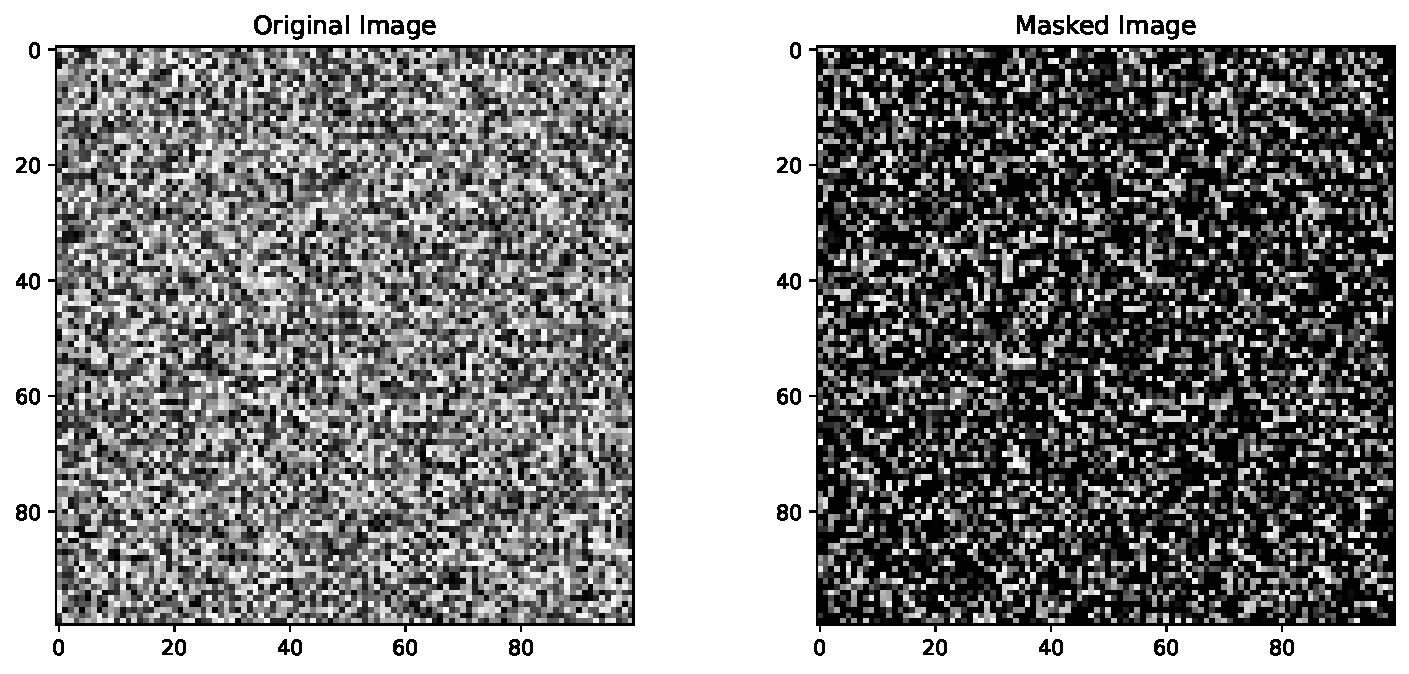
\includegraphics{module_2_files/figure-pdf/fig-imgmask-output-1.pdf}

}

\caption{\label{fig-imgmask}Demonstration of Masking in DIP using
Hadamard Product}

\end{figure}%

Application 2: Element-wise Scaling in Neural Networks

The Hadamard product can be used for dropout\footnote{A regularization
  techniques in Deep learning. This approach deactivate some selected
  neurons to control model over-fitting} in neural networks. A simple
simulated example is given below.

\begin{Shaded}
\begin{Highlighting}[]
\CommentTok{\# Simulated large activations (2D array) using NumPy}
\NormalTok{activations }\OperatorTok{=}\NormalTok{ np.random.rand(}\DecValTok{100}\NormalTok{, }\DecValTok{100}\NormalTok{)}

\CommentTok{\# Simulated dropout mask (binary matrix) using NumPy}
\NormalTok{dropout\_mask }\OperatorTok{=}\NormalTok{ np.random.randint(}\DecValTok{0}\NormalTok{, }\DecValTok{2}\NormalTok{, size}\OperatorTok{=}\NormalTok{(}\DecValTok{100}\NormalTok{, }\DecValTok{100}\NormalTok{))}

\CommentTok{\# Apply dropout}
\NormalTok{dropped\_activations }\OperatorTok{=}\NormalTok{ activations }\OperatorTok{*}\NormalTok{ dropout\_mask}

\CommentTok{\# Display results}
\BuiltInTok{print}\NormalTok{(}\StringTok{"Original Activations:"}\NormalTok{)}
\BuiltInTok{print}\NormalTok{(activations)}
\BuiltInTok{print}\NormalTok{(}\StringTok{"}\CharTok{\textbackslash{}n}\StringTok{Dropout Mask:"}\NormalTok{)}
\BuiltInTok{print}\NormalTok{(dropout\_mask)}
\BuiltInTok{print}\NormalTok{(}\StringTok{"}\CharTok{\textbackslash{}n}\StringTok{Dropped Activations:"}\NormalTok{)}
\BuiltInTok{print}\NormalTok{(dropped\_activations)}
\end{Highlighting}
\end{Shaded}

\begin{verbatim}
Original Activations:
[[1.50241810e-01 4.33985567e-01 8.06799811e-01 ... 3.17691660e-02
  2.65296312e-01 1.95520882e-01]
 [3.95437889e-01 2.63829859e-01 5.16712381e-01 ... 4.27303912e-01
  8.20997228e-01 4.15547921e-01]
 [5.98635672e-01 5.22905270e-01 8.08365101e-01 ... 7.49319840e-01
  3.02072551e-01 4.00749514e-01]
 ...
 [5.51947232e-01 7.93479508e-01 3.29339876e-01 ... 6.07145901e-01
  7.96351298e-01 3.83801103e-01]
 [8.97921944e-01 5.98465485e-01 2.37418723e-02 ... 1.44208520e-01
  6.93063855e-01 3.02194139e-01]
 [1.10657022e-01 4.26475997e-01 2.83044675e-02 ... 5.35278273e-04
  5.20851155e-01 2.01807675e-01]]

Dropout Mask:
[[1 0 0 ... 0 1 0]
 [0 1 0 ... 0 0 1]
 [0 1 0 ... 0 0 0]
 ...
 [1 1 0 ... 1 1 1]
 [1 0 0 ... 1 0 0]
 [0 0 1 ... 1 1 0]]

Dropped Activations:
[[1.50241810e-01 0.00000000e+00 0.00000000e+00 ... 0.00000000e+00
  2.65296312e-01 0.00000000e+00]
 [0.00000000e+00 2.63829859e-01 0.00000000e+00 ... 0.00000000e+00
  0.00000000e+00 4.15547921e-01]
 [0.00000000e+00 5.22905270e-01 0.00000000e+00 ... 0.00000000e+00
  0.00000000e+00 0.00000000e+00]
 ...
 [5.51947232e-01 7.93479508e-01 0.00000000e+00 ... 6.07145901e-01
  7.96351298e-01 3.83801103e-01]
 [8.97921944e-01 0.00000000e+00 0.00000000e+00 ... 1.44208520e-01
  0.00000000e+00 0.00000000e+00]
 [0.00000000e+00 0.00000000e+00 2.83044675e-02 ... 5.35278273e-04
  5.20851155e-01 0.00000000e+00]]
\end{verbatim}

Application 3: Statistical Data Analysis

In statistics, the Hadamard product can be applied to scale covariance
matrices. Here's how we can compute the covariance matrix using matrix
operations and apply scaling. Following \texttt{Python} code demonstrate
this.

\begin{Shaded}
\begin{Highlighting}[]
\ImportTok{import}\NormalTok{ sympy }\ImportTok{as}\NormalTok{ sp}
\ImportTok{import}\NormalTok{ numpy }\ImportTok{as}\NormalTok{ np}

\CommentTok{\# Simulated large dataset (2D array) using NumPy}
\NormalTok{data }\OperatorTok{=}\NormalTok{ np.random.rand(}\DecValTok{100}\NormalTok{, }\DecValTok{10}\NormalTok{)}

\CommentTok{\# Compute the mean of each column}
\NormalTok{mean }\OperatorTok{=}\NormalTok{ np.mean(data, axis}\OperatorTok{=}\DecValTok{0}\NormalTok{)}

\CommentTok{\# Center the data}
\NormalTok{centered\_data }\OperatorTok{=}\NormalTok{ data }\OperatorTok{{-}}\NormalTok{ mean}

\CommentTok{\# Compute the covariance matrix using matrix product operation}
\NormalTok{cov\_matrix }\OperatorTok{=}\NormalTok{ (centered\_data.T }\OperatorTok{@}\NormalTok{ centered\_data) }\OperatorTok{/}\NormalTok{ (centered\_data.shape[}\DecValTok{0}\NormalTok{] }\OperatorTok{{-}} \DecValTok{1}\NormalTok{)}
\NormalTok{cov\_matrix\_sympy }\OperatorTok{=}\NormalTok{ sp.Matrix(cov\_matrix)}

\CommentTok{\# Simulated scaling factors (2D array) using SymPy Matrix}
\NormalTok{scaling\_factors }\OperatorTok{=}\NormalTok{ sp.Matrix(np.random.rand(}\DecValTok{10}\NormalTok{, }\DecValTok{10}\NormalTok{))}

\CommentTok{\# Compute Hadamard product}
\NormalTok{scaled\_cov\_matrix }\OperatorTok{=}\NormalTok{ cov\_matrix\_sympy.multiply(scaling\_factors)}

\CommentTok{\# Display results}
\BuiltInTok{print}\NormalTok{(}\StringTok{"Covariance Matrix:"}\NormalTok{)}
\BuiltInTok{print}\NormalTok{(cov\_matrix\_sympy)}
\BuiltInTok{print}\NormalTok{(}\StringTok{"}\CharTok{\textbackslash{}n}\StringTok{Scaling Factors:"}\NormalTok{)}
\BuiltInTok{print}\NormalTok{(scaling\_factors)}
\BuiltInTok{print}\NormalTok{(}\StringTok{"}\CharTok{\textbackslash{}n}\StringTok{Scaled Covariance Matrix:"}\NormalTok{)}
\BuiltInTok{print}\NormalTok{(scaled\_cov\_matrix)}
\end{Highlighting}
\end{Shaded}

\begin{verbatim}
Covariance Matrix:
Matrix([[0.0829729792128583, -0.00130926119215640, -0.00449358582009456, -0.00854112365966432, -0.00329976113644906, 0.00249961852709112, -0.0120501743668226, 0.00847190395483982, -0.00250320880850894, -0.00217218949640616], [-0.00130926119215640, 0.0819209178948028, -0.00720443323906907, -0.00379571570606515, 0.00383404458466385, 0.00916815612381899, 0.00411350208051106, -0.00807198800287830, -3.78483431495599e-5, 0.00167081849986735], [-0.00449358582009456, -0.00720443323906907, 0.0758671540110243, 0.0185178056507831, -0.00150822954487172, -0.00846859757811348, 0.000922174597207738, 0.0135566295813176, -0.00570049318193161, 2.48134431911895e-5], [-0.00854112365966432, -0.00379571570606515, 0.0185178056507831, 0.0941261012619838, 0.00320923897828266, 0.00601688868132743, 0.0165742333077961, -0.000705126046065246, -0.00126050435883258, 0.000251714105107486], [-0.00329976113644906, 0.00383404458466385, -0.00150822954487172, 0.00320923897828266, 0.0745892709208168, 0.00478807324411202, 0.0126304845649463, 0.00753388592697854, 0.00233514906087995, 0.0116162268836834], [0.00249961852709112, 0.00916815612381899, -0.00846859757811348, 0.00601688868132743, 0.00478807324411202, 0.0991434262364808, 0.000967043743191874, 0.00798112851474827, 0.00743315745800000, 0.0191775166571220], [-0.0120501743668226, 0.00411350208051106, 0.000922174597207738, 0.0165742333077961, 0.0126304845649463, 0.000967043743191874, 0.0903454802843821, -0.00862478251249669, -0.0119424053824335, 0.00373324316687438], [0.00847190395483982, -0.00807198800287830, 0.0135566295813176, -0.000705126046065246, 0.00753388592697854, 0.00798112851474827, -0.00862478251249669, 0.0897438555945268, -0.00168869531060614, 0.00324084250836360], [-0.00250320880850894, -3.78483431495599e-5, -0.00570049318193161, -0.00126050435883258, 0.00233514906087995, 0.00743315745800000, -0.0119424053824335, -0.00168869531060614, 0.0859766773440997, 0.000397868786216571], [-0.00217218949640616, 0.00167081849986735, 2.48134431911895e-5, 0.000251714105107486, 0.0116162268836834, 0.0191775166571220, 0.00373324316687438, 0.00324084250836360, 0.000397868786216571, 0.0845716656424895]])

Scaling Factors:
Matrix([[0.529376470070988, 0.563200130818408, 0.318460183719583, 0.797238283210820, 0.216283871080610, 0.945573765224074, 0.368808118689262, 0.438858558355891, 0.0597040683479645, 0.0852507640650566], [0.694575003236391, 0.456902047158561, 0.520331227008267, 0.971286356060806, 0.624141762045315, 0.0110085767763656, 0.323216435775946, 0.743015856634809, 0.411911885266525, 0.0682024916225741], [0.573468980983563, 0.979319592731974, 0.292228532492185, 0.00828786205680987, 0.889129779669188, 0.905612206504996, 0.0251726195866563, 0.728665790859312, 0.374237787221140, 0.0869490312711454], [0.0615253470414977, 0.0146704437405060, 0.0480474155316687, 0.0902152657790595, 0.349422750680181, 0.632209642395382, 0.454973634702871, 0.247724827878588, 0.467884461465515, 0.0984644838484716], [0.725129571405943, 0.588888992047743, 0.539970831757330, 0.317065206390775, 0.551483037370507, 0.686979933427219, 0.304682398302593, 0.804144877757639, 0.458876190992004, 0.808763995940022], [0.839890935518173, 0.415779079129228, 0.633663702936697, 0.963268381124093, 0.383001122067917, 0.279297278104638, 0.349871120030461, 0.389571290434940, 0.260329138966151, 0.681723082162205], [0.405495357579473, 0.523030575656225, 0.926071368378906, 0.897134264764563, 0.612948535852914, 0.344566879670801, 0.269172250970144, 0.598518672204210, 0.453097308131964, 0.307293578076301], [0.791343025727367, 0.860995300866256, 0.591607185832944, 0.974148804991391, 0.676387777544676, 0.543093054153615, 0.560778274498421, 0.495456223524644, 0.368303989194053, 0.655674707056144], [0.362837079633854, 0.718929567452626, 0.266722287539223, 0.702653067393129, 0.481843996884993, 0.00331370681196930, 0.324406039005983, 0.730809379390980, 0.307117960367212, 0.647499721023504], [0.582963340163260, 0.882759702062714, 0.301649700660158, 0.896189027175441, 0.873001261684370, 0.807449880284280, 0.326216902761366, 0.720827703355635, 0.406977856266447, 0.251662351613438]])

Scaled Covariance Matrix:
Matrix([[0.0392621161636811, 0.0379768336785228, 0.0163507664815586, 0.0591680411074049, 0.00452797830944478, 0.0660914114880500, 0.0260346235625482, 0.0219607834951092, -0.00611934171818345, 0.00447221100087523], [0.0585630960979860, 0.0323003502888588, 0.0473290061830375, 0.0854675940260659, 0.0472428937520436, -0.00568321558995203, 0.0255762709782319, 0.0603982246176421, 0.0328992274880787, 0.0101938441147549], [0.0381055927130372, 0.0724162719832366, 0.0190611525222014, -0.00686614302762657, 0.0713922632100958, 0.0803650569641046, 0.00893588477803734, 0.0511526732602973, 0.0345941292523677, 0.00603973392918604], [0.0224854538465186, 0.0247403810554248, 0.0254559794136821, 0.0184847643417586, 0.0585070713429046, 0.0775715675571048, 0.0457361993390180, 0.0439976248508661, 0.0589011356742216, 0.0204665303765570], [0.0770596917095927, 0.0694048950669601, 0.0642483362361726, 0.0603536449580321, 0.0685320503086660, 0.0679946155277664, 0.0380172085875884, 0.0843146549277958, 0.0517354235757531, 0.0770107186338576], [0.110531319401127, 0.0710835109268010, 0.0821745729145992, 0.139442170068332, 0.0677629008155301, 0.0497561926232205, 0.0559591265723453, 0.0694915567985640, 0.0450440321317300, 0.0873246990763926], [0.0356502878243414, 0.0386164522682008, 0.0833062966661128, 0.0684321579367958, 0.0609565560355505, 0.0383322937468762, 0.0254615933049021, 0.0568430112017495, 0.0507328453131995, 0.0271541039969729], [0.0875729059684315, 0.0965090519389013, 0.0571841734576457, 0.0904434808531145, 0.0732437499498080, 0.0755366189693714, 0.0541380057046733, 0.0569955148650093, 0.0374046628233253, 0.0687296719987693], [0.0284868321118824, 0.0518996937024536, 0.0144211067962265, 0.0541165030703918, 0.0313731422146618, -0.00907237870803369, 0.0255192934935258, 0.0543157836145707, 0.0206523401174688, 0.0571131343175041], [0.0780955844462002, 0.0940677428828659, 0.0496131819150119, 0.104648247193575, 0.0929374312281347, 0.0828175090725600, 0.0406430392784513, 0.0822732135757534, 0.0484346025274588, 0.0472375217070637]])
\end{verbatim}

\subsubsection*{Practice Problems}\label{practice-problems}
\addcontentsline{toc}{subsubsection}{Practice Problems}

\textbf{Problem 1: Basic Hadamard Product}

Given matrices: \[A=\begin{bmatrix}1&2\\3&4\end{bmatrix}\]
\[B=\begin{bmatrix}5&6\\7&8\end{bmatrix}\]

Find the Hadamard product \(C=A\circ B\).

\textbf{Solution:}

\[C=\begin{bmatrix}1\cdot 5&2\cdot 6\\3\cdot7&4\cdot 8 \end{bmatrix}=\begin{bmatrix}5&12\\21&32\end{bmatrix}\]

\textbf{Problem 2: Hadamard Product with Identity Matrix}

Given matrices: \[A=\begin{bmatrix}1&2&3\\4&5&6\end{bmatrix}\]
\[I=\begin{bmatrix}1&0&0\\0&1&0\end{bmatrix}\]

Find the Hadamard product \(C=A\circ I\).

\textbf{Solution:}

\[C=\begin{bmatrix}1\cdot1&2\cdot 0&3\cdot 0\\4\cdot 0&5\cdot 1&6\cdot 0 \end{bmatrix}= \begin{bmatrix} 1&0&0\\0&5&0\end{bmatrix}\]

\textbf{Problem 3: Hadamard Product with Zero Matrix}

Given matrices: \[A=\begin{bmatrix}3&4\\5&6\end{bmatrix}\]
\[Z=\begin{bmatrix}0&0\\0&0\end{bmatrix}\]

Find the Hadamard product \(C=A\circ Z\).

\textbf{Solution:}

\[C=\begin{bmatrix}3\cdot 0&4\cdot 0\\ 5\cdot 0&6\cdot 0 \end{bmatrix}=\begin{bmatrix}0&0\\0&0\end{bmatrix}\]

\textbf{Problem 4: Hadamard Product of Two Identity Matrices}

Given identity matrices: \[I_2=\begin{bmatrix}1&0\\0&1\end{bmatrix}\]
\[I_3=\begin{bmatrix}1&0&0\\0&1&0\\0&0&1\end{bmatrix}\]

Find the Hadamard product \(C=I_2\circ I_3\) (extend \(I_2\) to match
dimensions of \(I_3\)).

\textbf{Solution:}

Extend \(I_2\) to \(I_3\):
\[I_2=\begin{bmatrix}1&0&0\\0&1&0\\0&0&0\end{bmatrix}\]

\[C=\begin{bmatrix}1\cdot 1&0\cdot 0&0\cdot 0\\0\cdot 0&1\cdot 1&0\cdot 0\\0\cdot 0&0\cdot 0&0\cdot 1\end{bmatrix}=\begin{bmatrix}1&0&0\\0&1&0\\0&0&0\end{bmatrix}\]

\textbf{Problem 5: Hadamard Product with Random Matrices}

Given random matrices: \[A=\begin{bmatrix}2&3\\1&4\end{bmatrix}\]
\[B=\begin{bmatrix}0&5\\6&2\end{bmatrix}\]

Find the Hadamard product \(C=A\circ B\).

\textbf{Solution:}

\[C=\begin{bmatrix}2\cdot 0&3\cdot 5\\1\cdot 6&4\cdot 2\end{bmatrix}=\begin{bmatrix}0&15\\6&8\end{bmatrix}\]

\textbf{Problem 6: Hadamard Product of 3x3 Matrices}

Given matrices: \[A=\begin{bmatrix}1&2&3\\4&5&6\\7&8&9\end{bmatrix}\]
\[B=\begin{bmatrix}9&8&7\\6&5&4\\3&2&1\end{bmatrix}\]

Find the Hadamard product \(C=A\circ B\).

\textbf{Solution:}

\[C=\begin{bmatrix}1\cdot 9&2\cdot 8&3\cdot 7\\4\cdot 6&5\cdot 5&6\cdot 4\\7\cdot 3&8\cdot 2&9\cdot 1\end{bmatrix}=\begin{bmatrix}9&16&21\\24&25&24\\21&16&9\end{bmatrix}\]

\textbf{Problem 7: Hadamard Product of Column Vectors}

Given column vectors: \[u=\begin{bmatrix}2\\3\end{bmatrix}\]
\[v=\begin{bmatrix}5\\6\end{bmatrix}\]

Find the Hadamard product \(w=u\circ v\).

\textbf{Solution:}

\[w=\begin{bmatrix}2\cdot 5\\3\cdot 6\end{bmatrix}=\begin{bmatrix}10\\18\end{bmatrix}\]

\textbf{Problem 8: Hadamard Product with Non-Square Matrices}

Given matrices: \[A=\begin{bmatrix}1&2\\3&4\\5&6\end{bmatrix}\]
\[B=\begin{bmatrix}7&8\\9&10\end{bmatrix}\]

Find the Hadamard product \(C=A\circ B\) (extend \(B\) to match
dimensions of \(A\)).

\textbf{Solution:}

Extend \(B\) to match dimensions of \(A\):
\[B=\begin{bmatrix}7&8\\9&10\\7&8\end{bmatrix}\]

\[C=\begin{bmatrix}1\cdot 7&2\cdot 8\\3\cdot 9&4\cdot 10\\5\cdot 7&6\cdot 8\end{bmatrix}=\begin{bmatrix}7&16\\27&40\\35&48\end{bmatrix}\]

\textbf{Problem 9: Hadamard Product in Image Processing}

Given matrices representing image pixel values:
\[A=\begin{bmatrix}10&20\\30&40\end{bmatrix}\]
\[B=\begin{bmatrix}0.5&1.5\\2.0&0.5\end{bmatrix}\]

Find the Hadamard product \(C=A\circ B\).

\textbf{Solution:}

\[C=\begin{bmatrix}10\cdot 0.5&20\cdot 1.5\\30\cdot 2.0&40\cdot 0.5\end{bmatrix}=\begin{bmatrix}5&30\\60&20\end{bmatrix}\]

\textbf{Problem 10: Hadamard Product in Statistical Data}

Given matrices representing two sets of statistical data:

\[A=\begin{bmatrix}5&6&7\\8&9&10\end{bmatrix}\]
\[B=\begin{bmatrix}1&2&3\\4&5&6\end{bmatrix}\]

Find the Hadamard product \(C=A\circ B\).

\textbf{Solution:}

\[C=\begin{bmatrix}5\cdot 1&6\cdot 2&7\cdot 3\\8\cdot 4&9\cdot 5&10\cdot 6\end{bmatrix}=\begin{bmatrix}5&12&21\\32&45&60\end{bmatrix}\]

\subsubsection*{Inner Product of
Matrices}\label{inner-product-of-matrices}
\addcontentsline{toc}{subsubsection}{Inner Product of Matrices}

The inner product of two matrices is a generalized extension of the dot
product, where each matrix is treated as a vector in a high-dimensional
space. For two matrices \(A\) and \(B\) of the same dimension
\(m \times n\), the inner product is defined as the sum of the
element-wise products of the matrices.

\begin{tcolorbox}[enhanced jigsaw, leftrule=.75mm, bottomtitle=1mm, colback=white, toptitle=1mm, opacitybacktitle=0.6, toprule=.15mm, colbacktitle=quarto-callout-important-color!10!white, arc=.35mm, colframe=quarto-callout-important-color-frame, title=\textcolor{quarto-callout-important-color}{\faExclamation}\hspace{0.5em}{Definition (Inner product)}, titlerule=0mm, rightrule=.15mm, left=2mm, bottomrule=.15mm, breakable, coltitle=black, opacityback=0]

For two matrices \(A\) and \(B\) of dimension \(m \times n\), the inner
product \(\langle A, B \rangle\) is given by:

\[\langle A, B \rangle = \sum_{i=1}^{m} \sum_{j=1}^{n} A_{ij} \cdot B_{ij}\]

where \(\cdot\) denotes element-wise multiplication.

\end{tcolorbox}

\begin{tcolorbox}[enhanced jigsaw, leftrule=.75mm, bottomtitle=1mm, colback=white, toptitle=1mm, opacitybacktitle=0.6, toprule=.15mm, colbacktitle=quarto-callout-important-color!10!white, arc=.35mm, colframe=quarto-callout-important-color-frame, title=\textcolor{quarto-callout-important-color}{\faExclamation}\hspace{0.5em}{Properties}, titlerule=0mm, rightrule=.15mm, left=2mm, bottomrule=.15mm, breakable, coltitle=black, opacityback=0]

\begin{enumerate}
\def\labelenumi{\arabic{enumi}.}
\item
  \textbf{Commutativity}:
  \[\langle A, B \rangle = \langle B, A \rangle\]
\item
  \textbf{Linearity}:
  \[\langle A + C, B \rangle = \langle A, B \rangle + \langle C, B \rangle\]
\item
  \textbf{Positive Definiteness}: \[\langle A, A \rangle \geq 0\] with
  equality if and only if \(A\) is a zero matrix.
\end{enumerate}

\end{tcolorbox}

Some simple examples showing the mathematical process of calculating the
inner product is given bellow.

\textbf{Example 1: Basic Inner Product}

Given matrices:

\[A = \begin{pmatrix}1 & 2 \\3 & 4\end{pmatrix}, \quad B = \begin{pmatrix}5 & 6 \\7 & 8\end{pmatrix}\]

The inner product \(\langle A, B \rangle\) is:

\[\langle A, B \rangle = 1 \cdot 5 + 2 \cdot 6 + 3 \cdot 7 + 4 \cdot 8 = 5 + 12 + 21 + 32 = 70\]

\textbf{Example 2: Inner Product with Larger Matrices}

Given matrices:

\[A = \begin{pmatrix}1 & 2 & 3 \\4 & 5 & 6 \\7 & 8 & 9\end{pmatrix}, \quad B = \begin{pmatrix}9 & 8 & 7 \\6 & 5 & 4 \\3 & 2 & 1\end{pmatrix}\]

The inner product \(\langle A, B \rangle\) is calculated as:
\begin{align*}
\langle A, B \rangle &= 1 \cdot 9 + 2 \cdot 8 + 3 \cdot 7 + 4 \cdot 6 + 5 \cdot 5 + 6 \cdot 4 + 7 \cdot 3 + 8 \cdot 2 + 9 \cdot 1\\
&= 9 + 16 + 21 + 24 + 25 + 24 + 21 + 16 + 9\\
&= 175
\end{align*}

\subsubsection*{Practice Problems}\label{practice-problems-1}
\addcontentsline{toc}{subsubsection}{Practice Problems}

\textbf{Problem 1: Inner Product of 2x2 Matrices}

Given matrices: \[A=\begin{bmatrix}1&2\\3&4\end{bmatrix}\]
\[B=\begin{bmatrix}5&6\\7&8\end{bmatrix}\]

\textbf{Solution:}

\begin{align*}
\langle A,B \rangle &= \sum_{i,j} A_{ij} B_{ij} \\
&= 1\cdot5 + 2\cdot6 + 3\cdot7 + 4\cdot8 \\
&= 5 + 12 + 21 + 32 \\
&= 70
\end{align*}

\begin{center}\rule{0.5\linewidth}{0.5pt}\end{center}

\textbf{Problem 2: Inner Product of 3x3 Matrices}

Given matrices: \[A=\begin{bmatrix}1&0&2\\3&4&5\\6&7&8\end{bmatrix}\]
\[B=\begin{bmatrix}8&7&6\\5&4&3\\2&1&0\end{bmatrix}\]

\textbf{Solution:}

\begin{align*}
\langle A,B \rangle &= \sum_{i,j} A_{ij} B_{ij} \\
&= 1\cdot8 + 0\cdot7 + 2\cdot6 + \\
&\quad 3\cdot5 + 4\cdot4 + 5\cdot3 + \\
&\quad 6\cdot2 + 7\cdot1 + 8\cdot0 \\
&= 8 + 0 + 12 + 15 + 16 + 15 + 12 + 7 + 0 \\
&= 85
\end{align*}

\begin{center}\rule{0.5\linewidth}{0.5pt}\end{center}

\textbf{Problem 3: Inner Product of Diagonal Matrices}

Given diagonal matrices:
\[A=\begin{bmatrix}2&0&0\\0&3&0\\0&0&4\end{bmatrix}\]
\[B=\begin{bmatrix}5&0&0\\0&6&0\\0&0&7\end{bmatrix}\]

\textbf{Solution:}

\begin{align*}
\langle A,B \rangle &= \sum_{i,j} A_{ij} B_{ij} \\
&= 2\cdot5 + 0\cdot0 + 0\cdot0 + \\
&\quad 0\cdot0 + 3\cdot6 + 0\cdot0 + \\
&\quad 0\cdot0 + 0\cdot0 + 4\cdot7 \\
&= 10 + 0 + 0 + 0 + 18 + 0 + 0 + 0 + 28 \\
&= 56
\end{align*}

\begin{center}\rule{0.5\linewidth}{0.5pt}\end{center}

\textbf{Problem 4: Inner Product of Column Vectors}

Given column vectors: \[u=\begin{bmatrix}1\\2\\3\end{bmatrix}\]
\[v=\begin{bmatrix}4\\5\\6\end{bmatrix}\]

\textbf{Solution:}

\begin{align*}
\langle u,v \rangle &= \sum_{i} u_i v_i \\
&= 1\cdot4 + 2\cdot5 + 3\cdot6 \\
&= 4 + 10 + 18 \\
&= 32
\end{align*}

\begin{center}\rule{0.5\linewidth}{0.5pt}\end{center}

\textbf{Problem 5: Inner Product with Random Matrices}

Given matrices: \[A=\begin{bmatrix}3&2\\1&4\end{bmatrix}\]
\[B=\begin{bmatrix}5&7\\8&6\end{bmatrix}\]

\textbf{Solution:}

\begin{align*}
\langle A,B \rangle &= \sum_{i,j} A_{ij} B_{ij} \\
&= 3\cdot5 + 2\cdot7 + \\
&\quad 1\cdot8 + 4\cdot6 \\
&= 15 + 14 + 8 + 24 \\
&= 61
\end{align*}

\begin{center}\rule{0.5\linewidth}{0.5pt}\end{center}

\textbf{Problem 6: Inner Product of 2x3 and 3x2 Matrices}

Given matrices: \[A=\begin{bmatrix}1&2&3\\4&5&6\end{bmatrix}\]
\[B=\begin{bmatrix}7&8\\9&10\\11&12\end{bmatrix}\]

\textbf{Solution:}

\begin{align*}
\langle A,B \rangle &= \sum_{i,j} A_{ij} B_{ij} \\
&= 1\cdot7 + 2\cdot8 + 3\cdot11 + \\
&\quad 4\cdot9 + 5\cdot10 + 6\cdot12 \\
&= 7 + 16 + 33 + 36 + 50 + 72 \\
&= 214
\end{align*}

\begin{center}\rule{0.5\linewidth}{0.5pt}\end{center}

\textbf{Problem 7: Inner Product with Transpose Operation}

Given matrices: \[A=\begin{bmatrix}2&3\\4&5\end{bmatrix}\]
\[B=\begin{bmatrix}6&7\\8&9\end{bmatrix}\]

\textbf{Solution:}

\begin{align*}
\langle A,B \rangle &= \sum_{i,j} A_{ij} B_{ij} \\
&= 2\cdot6 + 3\cdot7 + \\
&\quad 4\cdot8 + 5\cdot9 \\
&= 12 + 21 + 32 + 45 \\
&= 110
\end{align*}

\begin{center}\rule{0.5\linewidth}{0.5pt}\end{center}

\textbf{Problem 8: Inner Product of Symmetric Matrices}

Given symmetric matrices: \[A=\begin{bmatrix}1&2\\2&3\end{bmatrix}\]
\[B=\begin{bmatrix}4&5\\5&6\end{bmatrix}\]

\textbf{Solution:}

\begin{align*}
\langle A,B \rangle &= \sum_{i,j} A_{ij} B_{ij} \\
&= 1\cdot4 + 2\cdot5 + \\
&\quad 2\cdot5 + 3\cdot6 \\
&= 4 + 10 + 10 + 18 \\
&= 42
\end{align*}

\begin{center}\rule{0.5\linewidth}{0.5pt}\end{center}

\textbf{Problem 9: Inner Product with Complex Matrices}

Given matrices: \[A=\begin{bmatrix}1+i&2-i\\3+i&4-i\end{bmatrix}\]
\[B=\begin{bmatrix}5-i&6+i\\7-i&8+i\end{bmatrix}\]

\textbf{Solution:}

\begin{align*}
\langle A,B \rangle &= \sum_{i,j} \text{Re}(A_{ij} \overline{B_{ij}}) \\
&= (1+i)\cdot(5+i) + (2-i)\cdot(6-i) + \\
&\quad (3+i)\cdot(7+i) + (4-i)\cdot(8+i) \\
&= (5+i+5i-i^2) + (12-i-6i+i^2) + \\
&\quad (21+i+7i-i^2) + (32+i-8i-i^2) \\
&= 5+5 + 12 - 6 + 21 + 32 - 2 \\
&= 62
\end{align*}

\begin{center}\rule{0.5\linewidth}{0.5pt}\end{center}

\textbf{Problem 10: Inner Product of 4x4 Matrices}

Given matrices:
\[A=\begin{bmatrix}1&2&3&4\\5&6&7&8\\9&10&11&12\\13&14&15&16\end{bmatrix}\]
\[B=\begin{bmatrix}16&15&14&13\\12&11&10&9\\8&7&6&5\\4&3&2&1\end{bmatrix}\]

\textbf{Solution:}

\begin{align*}
\langle A,B \rangle &= \sum_{i,j} A_{ij} B_{ij} \\
&= 1\cdot16 + 2\cdot15 + 3\cdot14 + 4\cdot13 + \\
&\quad 5\cdot12 + 6\cdot11 + 7\cdot10 + 8\cdot9 + \\
&\quad 9\cdot8 + 10\cdot7 + 11\cdot6 + 12\cdot5 + \\
&\quad 13\cdot4 + 14\cdot3 + 15\cdot2 + 16\cdot1 \\
&= 16 + 30 + 42 + 52 + 60 + 66 + 70 + 72 + \\
&\quad 72 + 70 + 66 + 60 + 52 + 42 + 30 + 16 \\
&= 696
\end{align*}

\begin{center}\rule{0.5\linewidth}{0.5pt}\end{center}

Now let's look into the computational part of \emph{inner product}.

\begin{enumerate}
\def\labelenumi{\arabic{enumi}.}
\tightlist
\item
  Compute Inner Product from Scratch (without Libraries)
\end{enumerate}

Here's how you can compute the inner product from the scratch:

\begin{Shaded}
\begin{Highlighting}[]
\CommentTok{\# Define matrices A and B}
\NormalTok{A }\OperatorTok{=}\NormalTok{ [[}\DecValTok{1}\NormalTok{, }\DecValTok{2}\NormalTok{, }\DecValTok{3}\NormalTok{], [}\DecValTok{4}\NormalTok{, }\DecValTok{5}\NormalTok{, }\DecValTok{6}\NormalTok{]]}
\NormalTok{B }\OperatorTok{=}\NormalTok{ [[}\DecValTok{7}\NormalTok{, }\DecValTok{8}\NormalTok{, }\DecValTok{9}\NormalTok{], [}\DecValTok{10}\NormalTok{, }\DecValTok{11}\NormalTok{, }\DecValTok{12}\NormalTok{]]}

\CommentTok{\# Function to compute inner product}
\KeywordTok{def}\NormalTok{ inner\_product(A, B):}
    \CommentTok{\# Get the number of rows and columns}
\NormalTok{    num\_rows }\OperatorTok{=} \BuiltInTok{len}\NormalTok{(A)}
\NormalTok{    num\_cols }\OperatorTok{=} \BuiltInTok{len}\NormalTok{(A[}\DecValTok{0}\NormalTok{])}
    
    \CommentTok{\# Initialize the result}
\NormalTok{    result }\OperatorTok{=} \DecValTok{0}
    
    \CommentTok{\# Compute the inner product}
    \ControlFlowTok{for}\NormalTok{ i }\KeywordTok{in} \BuiltInTok{range}\NormalTok{(num\_rows):}
        \ControlFlowTok{for}\NormalTok{ j }\KeywordTok{in} \BuiltInTok{range}\NormalTok{(num\_cols):}
\NormalTok{            result }\OperatorTok{+=}\NormalTok{ A[i][j] }\OperatorTok{*}\NormalTok{ B[i][j]}
    
    \ControlFlowTok{return}\NormalTok{ result}

\CommentTok{\# Compute inner product}
\NormalTok{inner\_product\_result }\OperatorTok{=}\NormalTok{ inner\_product(A, B)}

\CommentTok{\# Display result}
\BuiltInTok{print}\NormalTok{(}\StringTok{"Inner Product (From Scratch):"}\NormalTok{)}
\BuiltInTok{print}\NormalTok{(inner\_product\_result)}
\end{Highlighting}
\end{Shaded}

\begin{verbatim}
Inner Product (From Scratch):
217
\end{verbatim}

\begin{enumerate}
\def\labelenumi{\arabic{enumi}.}
\setcounter{enumi}{1}
\tightlist
\item
  Compute Inner Product Using \texttt{NumPy}
\end{enumerate}

Here's how to compute the inner product using Numpy:

\begin{Shaded}
\begin{Highlighting}[]
\ImportTok{import}\NormalTok{ numpy }\ImportTok{as}\NormalTok{ np}
\CommentTok{\# Define matrices A and B}
\NormalTok{A }\OperatorTok{=}\NormalTok{ np.array([[}\DecValTok{1}\NormalTok{, }\DecValTok{2}\NormalTok{, }\DecValTok{3}\NormalTok{], [}\DecValTok{4}\NormalTok{, }\DecValTok{5}\NormalTok{, }\DecValTok{6}\NormalTok{]])}
\NormalTok{B }\OperatorTok{=}\NormalTok{ np.array([[}\DecValTok{7}\NormalTok{, }\DecValTok{8}\NormalTok{, }\DecValTok{9}\NormalTok{], [}\DecValTok{10}\NormalTok{, }\DecValTok{11}\NormalTok{, }\DecValTok{12}\NormalTok{]])}
\CommentTok{\# calculating innerproduct}
\NormalTok{inner\_product }\OperatorTok{=}\NormalTok{ (A}\OperatorTok{*}\NormalTok{B).}\BuiltInTok{sum}\NormalTok{() }\CommentTok{\# calculate element{-}wise product, then column sum}

\BuiltInTok{print}\NormalTok{(}\StringTok{"Inner Product (Using numpy):"}\NormalTok{)}
\BuiltInTok{print}\NormalTok{(inner\_product)}
\end{Highlighting}
\end{Shaded}

\begin{verbatim}
Inner Product (Using numpy):
217
\end{verbatim}

The same operation can be done using \texttt{SymPy} functions as
follows.

\begin{Shaded}
\begin{Highlighting}[]
\ImportTok{import}\NormalTok{ sympy }\ImportTok{as}\NormalTok{ sp}
\ImportTok{import}\NormalTok{ numpy }\ImportTok{as}\NormalTok{ np  }
\CommentTok{\# Define matrices A and B}
\NormalTok{A }\OperatorTok{=}\NormalTok{ sp.Matrix([[}\DecValTok{1}\NormalTok{, }\DecValTok{2}\NormalTok{, }\DecValTok{3}\NormalTok{], [}\DecValTok{4}\NormalTok{, }\DecValTok{5}\NormalTok{, }\DecValTok{6}\NormalTok{]])}
\NormalTok{B }\OperatorTok{=}\NormalTok{ sp.Matrix([[}\DecValTok{7}\NormalTok{, }\DecValTok{8}\NormalTok{, }\DecValTok{9}\NormalTok{], [}\DecValTok{10}\NormalTok{, }\DecValTok{11}\NormalTok{, }\DecValTok{12}\NormalTok{]])}

\CommentTok{\# Compute element{-}wise product}
\NormalTok{elementwise\_product }\OperatorTok{=}\NormalTok{ A.multiply\_elementwise(B)}

\CommentTok{\# Calculate sum of each column}
\NormalTok{inner\_product\_sympy }\OperatorTok{=}\NormalTok{ np.}\BuiltInTok{sum}\NormalTok{(elementwise\_product)}

\CommentTok{\# Display result}
\BuiltInTok{print}\NormalTok{(}\StringTok{"Inner Product (Using SymPy):"}\NormalTok{)}
\BuiltInTok{print}\NormalTok{(inner\_product\_sympy)}
\end{Highlighting}
\end{Shaded}

\begin{verbatim}
Inner Product (Using SymPy):
217
\end{verbatim}

A vector dot product (in Physics) can be calculated using \texttt{SymPy}
\texttt{.dot()} function as shown below.

Let \(A=\begin{pmatrix}1&2&3\end{pmatrix}\) and
\(B=\begin{pmatrix}4&5&6\end{pmatrix}\), then the dot product,
\(A\cdot B\) is computed as:

\begin{Shaded}
\begin{Highlighting}[]
\ImportTok{import}\NormalTok{ sympy }\ImportTok{as}\NormalTok{ sp}
\NormalTok{A}\OperatorTok{=}\NormalTok{sp.Matrix([}\DecValTok{1}\NormalTok{,}\DecValTok{2}\NormalTok{,}\DecValTok{3}\NormalTok{])}
\NormalTok{B}\OperatorTok{=}\NormalTok{sp.Matrix([}\DecValTok{4}\NormalTok{,}\DecValTok{5}\NormalTok{,}\DecValTok{6}\NormalTok{])}
\NormalTok{display(A.dot(B)) }\CommentTok{\# calculate fot product of A and B}
\end{Highlighting}
\end{Shaded}

$\displaystyle 32$

\begin{tcolorbox}[enhanced jigsaw, leftrule=.75mm, bottomtitle=1mm, colback=white, toptitle=1mm, opacitybacktitle=0.6, toprule=.15mm, colbacktitle=quarto-callout-warning-color!10!white, arc=.35mm, colframe=quarto-callout-warning-color-frame, title=\textcolor{quarto-callout-warning-color}{\faExclamationTriangle}\hspace{0.5em}{A word of caution}, titlerule=0mm, rightrule=.15mm, left=2mm, bottomrule=.15mm, breakable, coltitle=black, opacityback=0]

In \texttt{SymPy} , \texttt{sp.Matrix({[}1,2,3{]})} create a column
vector. But \texttt{np.array({[}1,2,3{]})} creates a row vector. So be
careful while applying matrix/ dot product operations on these objects.

\end{tcolorbox}

The same dot product using \texttt{numpy} object can be done as follows:

\begin{Shaded}
\begin{Highlighting}[]
\ImportTok{import}\NormalTok{ numpy }\ImportTok{as}\NormalTok{ np}
\NormalTok{A}\OperatorTok{=}\NormalTok{np.array([}\DecValTok{1}\NormalTok{,}\DecValTok{2}\NormalTok{,}\DecValTok{3}\NormalTok{])}
\NormalTok{B}\OperatorTok{=}\NormalTok{np.array([}\DecValTok{4}\NormalTok{,}\DecValTok{5}\NormalTok{,}\DecValTok{6}\NormalTok{])}
\NormalTok{display(A.dot(B.T))}\CommentTok{\# dot() stands for dot product B.T represents the transpose of B}
\end{Highlighting}
\end{Shaded}

\begin{verbatim}
np.int64(32)
\end{verbatim}

\textbf{Practical Applications}

Application 1: Signal Processing

In signal processing, the inner product can be used to measure the
similarity between two signals. Here the most popular measure of
similarity is the \texttt{cosine} similarity. This measure is defined
as:

\[\cos \theta=\dfrac{A\cdot B}{||A|| ||B||}\]

Now consider two digital signals are given. It's cosine similarity
measure can be calculated with a simulated data as shown below.

\begin{Shaded}
\begin{Highlighting}[]
\ImportTok{import}\NormalTok{ numpy }\ImportTok{as}\NormalTok{ np}

\CommentTok{\# Simulated large signals (1D array) using NumPy}
\NormalTok{signal1 }\OperatorTok{=}\NormalTok{ np.sin(np.random.rand(}\DecValTok{1000}\NormalTok{))}
\NormalTok{signal2 }\OperatorTok{=}\NormalTok{ np.cos(np.random.rand(}\DecValTok{1000}\NormalTok{))}

\CommentTok{\# Compute inner product}
\NormalTok{inner\_product\_signal }\OperatorTok{=}\NormalTok{ np.dot(signal1, signal2)}
\CommentTok{\#cosine\_sim=np.dot(signal1,signal2)/(np.linalg.norm(signal1)*np.linalg.norm(signal2))}
\CommentTok{\# Display result}
\NormalTok{cosine\_sim}\OperatorTok{=}\NormalTok{inner\_product\_signal}\OperatorTok{/}\NormalTok{(np.sqrt(np.dot(signal1,signal1))}\OperatorTok{*}\NormalTok{np.sqrt(np.dot(signal2,signal2)))}
\BuiltInTok{print}\NormalTok{(}\StringTok{"Inner Product (Using numpy):"}\NormalTok{)}
\BuiltInTok{print}\NormalTok{(inner\_product\_signal)}
\BuiltInTok{print}\NormalTok{(}\StringTok{"Similarity of signals:"}\NormalTok{)}
\BuiltInTok{print}\NormalTok{(cosine\_sim)}
\end{Highlighting}
\end{Shaded}

\begin{verbatim}
Inner Product (Using numpy):
376.2416744359054
Similarity of signals:
0.8656766327701758
\end{verbatim}

Application 2: Machine Learning - Feature Similarity

In machine learning, the inner product is used to calculate the
similarity between feature vectors.

\begin{Shaded}
\begin{Highlighting}[]
\ImportTok{import}\NormalTok{ numpy }\ImportTok{as}\NormalTok{ np}

\CommentTok{\# Simulated feature vectors (2D array) using NumPy}
\NormalTok{features1 }\OperatorTok{=}\NormalTok{ np.random.rand(}\DecValTok{100}\NormalTok{, }\DecValTok{10}\NormalTok{)}
\NormalTok{features2 }\OperatorTok{=}\NormalTok{ np.random.rand(}\DecValTok{100}\NormalTok{, }\DecValTok{10}\NormalTok{)}

\CommentTok{\# Compute inner product for each feature vector}
\NormalTok{inner\_products }\OperatorTok{=}\NormalTok{ np.einsum(}\StringTok{\textquotesingle{}ij,ij{-}\textgreater{}i\textquotesingle{}}\NormalTok{, features1, features2) }\CommentTok{\# use Einstien\textquotesingle{}s sum}

\CommentTok{\# Display results}
\BuiltInTok{print}\NormalTok{(}\StringTok{"Inner Products of Feature Vectors:"}\NormalTok{)}
\NormalTok{display(inner\_products)}
\end{Highlighting}
\end{Shaded}

\begin{verbatim}
Inner Products of Feature Vectors:
\end{verbatim}

\begin{verbatim}
array([1.86618745, 2.51274116, 3.22480512, 1.75063304, 2.71721823,
       1.98680212, 2.49529215, 2.71034517, 2.13720204, 2.11147807,
       1.96657719, 3.5413832 , 1.79540191, 3.70295428, 3.65000013,
       2.73129036, 2.73390532, 2.72873231, 2.16813032, 2.70008207,
       2.5691309 , 3.8267985 , 2.92428261, 3.70546606, 1.76740125,
       1.87750167, 2.6071815 , 2.84333663, 2.18774745, 1.12079554,
       1.57466902, 1.64387872, 2.90078842, 1.99736669, 2.89345103,
       3.27215634, 1.15500698, 3.4420285 , 2.66379682, 1.97189201,
       2.69580422, 3.66770217, 2.17603749, 2.64082386, 1.84436202,
       2.52202546, 3.69840123, 2.65554438, 2.56514562, 3.30404738,
       2.9149493 , 3.20316329, 1.67700272, 2.56251505, 2.13654397,
       2.58640145, 2.0852157 , 1.729585  , 2.00190409, 2.36285034,
       1.89257731, 2.76695102, 2.22617247, 3.38664877, 2.44943569,
       3.23633599, 2.78761947, 2.42658745, 1.9870498 , 2.14063901,
       1.8996319 , 1.78367225, 2.55715996, 2.31152679, 2.77771334,
       1.62328576, 1.7009172 , 3.26510025, 3.36515712, 2.73481074,
       2.34406789, 1.77924725, 3.06492737, 1.87634451, 2.40285279,
       2.26284099, 2.40946304, 1.95833024, 3.13335721, 3.12926964,
       2.5930494 , 1.01589811, 1.54176088, 1.8962135 , 1.9040875 ,
       2.16756144, 1.2903262 , 2.26065421, 4.28424505, 1.82733956])
\end{verbatim}

Application 3: Covariance Matrix in Statistics

The inner product can be used to compute covariance matrices for
statistical data analysis. If \(X\) is a given distribution and
\(x=X-\bar{X}\). Then the covariance of \(X\) can be calculated as
\(cov(X)=\dfrac{1}{n-1}(x\cdot x^T)\) \footnote{Remember that the
  covariance of \(X\) is defined as
  \(Cov(X)=\dfrac{\sum (X-\bar{X})^2}{n-1}\)}. The python code a
simulated data is shown below.

\begin{Shaded}
\begin{Highlighting}[]
\ImportTok{import}\NormalTok{ sympy }\ImportTok{as}\NormalTok{ sp}
\ImportTok{import}\NormalTok{ numpy }\ImportTok{as}\NormalTok{ np}

\CommentTok{\# Simulated large dataset (2D array) using NumPy}
\NormalTok{data }\OperatorTok{=}\NormalTok{ np.random.rand(}\DecValTok{100}\NormalTok{, }\DecValTok{10}\NormalTok{)}

\CommentTok{\# Compute the mean of each column}
\NormalTok{mean }\OperatorTok{=}\NormalTok{ np.mean(data, axis}\OperatorTok{=}\DecValTok{0}\NormalTok{)}

\CommentTok{\# Center the data}
\NormalTok{centered\_data }\OperatorTok{=}\NormalTok{ data }\OperatorTok{{-}}\NormalTok{ mean}

\CommentTok{\# Compute the covariance matrix using matrix product operation}
\NormalTok{cov\_matrix }\OperatorTok{=}\NormalTok{ (centered\_data.T }\OperatorTok{@}\NormalTok{ centered\_data) }\OperatorTok{/}\NormalTok{ (centered\_data.shape[}\DecValTok{0}\NormalTok{] }\OperatorTok{{-}} \DecValTok{1}\NormalTok{)}
\NormalTok{cov\_matrix\_sympy }\OperatorTok{=}\NormalTok{ sp.Matrix(cov\_matrix)}

\CommentTok{\# Display results}
\BuiltInTok{print}\NormalTok{(}\StringTok{"Covariance Matrix:"}\NormalTok{)}
\NormalTok{display(cov\_matrix\_sympy)}
\end{Highlighting}
\end{Shaded}

\begin{verbatim}
Covariance Matrix:
\end{verbatim}

$\displaystyle \left[\begin{matrix}0.0688323944026016 & 0.0153740605980509 & -0.000140933353214011 & 0.00920489541395922 & -0.00387734773004558 & -0.00571190548041544 & -0.0049428689590279 & -0.00463812193721968 & 0.0105897102719774 & 0.000992217456020462\\0.0153740605980509 & 0.0905182214346242 & 0.000712744651254393 & -0.00436319787429453 & -0.000825052380333573 & 0.00786460769477729 & -7.22532226030962 \cdot 10^{-5} & -0.00028578801387221 & 0.00456567668280999 & -0.000925756164661477\\-0.000140933353214011 & 0.000712744651254393 & 0.0585555577321913 & -0.00452162693037121 & 0.00126191421665622 & 0.00217942019679709 & 0.000750926068297655 & -0.00674883183942774 & 0.00612207233520953 & -0.0137231192102392\\0.00920489541395922 & -0.00436319787429453 & -0.00452162693037121 & 0.0862201676624409 & 0.0141142358813661 & -0.0044274235853324 & 0.00328828339659587 & -0.00724495179921262 & 0.00795687838697261 & -0.00242695079854651\\-0.00387734773004558 & -0.000825052380333573 & 0.00126191421665622 & 0.0141142358813661 & 0.0704130064243136 & -0.00248709243136213 & -0.00705058277161529 & -0.0125027947605104 & 0.000410096922416119 & 0.00381441562686544\\-0.00571190548041544 & 0.00786460769477729 & 0.00217942019679709 & -0.0044274235853324 & -0.00248709243136213 & 0.0792763589927339 & 0.0153086477835871 & 0.00455611728990078 & 0.00821017903350576 & -0.0126677750951018\\-0.0049428689590279 & -7.22532226030962 \cdot 10^{-5} & 0.000750926068297655 & 0.00328828339659587 & -0.00705058277161529 & 0.0153086477835871 & 0.0959574353313151 & -0.0127859615200589 & 0.00211389754260556 & 0.00362563895510698\\-0.00463812193721968 & -0.00028578801387221 & -0.00674883183942774 & -0.00724495179921262 & -0.0125027947605104 & 0.00455611728990078 & -0.0127859615200589 & 0.0941193122583523 & -0.0111370988138436 & 0.00345814477445709\\0.0105897102719774 & 0.00456567668280999 & 0.00612207233520953 & 0.00795687838697261 & 0.000410096922416119 & 0.00821017903350576 & 0.00211389754260556 & -0.0111370988138436 & 0.0783537998017076 & -0.0158495541158567\\0.000992217456020462 & -0.000925756164661477 & -0.0137231192102392 & -0.00242695079854651 & 0.00381441562686544 & -0.0126677750951018 & 0.00362563895510698 & 0.00345814477445709 & -0.0158495541158567 & 0.0838018781279234\end{matrix}\right]$

These examples demonstrate the use of inner product and dot product in
various applications.

\subsubsection*{Outer Product}\label{outer-product}
\addcontentsline{toc}{subsubsection}{Outer Product}

The outer product of two vectors results in a matrix, and it is a way to
combine these vectors into a higher-dimensional representation.

\begin{tcolorbox}[enhanced jigsaw, leftrule=.75mm, bottomtitle=1mm, colback=white, toptitle=1mm, opacitybacktitle=0.6, toprule=.15mm, colbacktitle=quarto-callout-note-color!10!white, arc=.35mm, colframe=quarto-callout-note-color-frame, title=\textcolor{quarto-callout-note-color}{\faInfo}\hspace{0.5em}{Definition (Outer Product)}, titlerule=0mm, rightrule=.15mm, left=2mm, bottomrule=.15mm, breakable, coltitle=black, opacityback=0]

For two vectors \(\mathbf{u}\) and \(\mathbf{v}\) of dimensions \(m\)
and \(n\) respectively, the outer product
\(\mathbf{u} \otimes \mathbf{v}\) is an \(m \times n\) matrix defined
as:

\[(\mathbf{u} \otimes \mathbf{v})_{ij} = u_i \cdot v_j\]

where \(\cdot\) denotes the outer product operation. In matrix notation,
for two column vectors \(u,v\), \[u\otimes v=uv^T\]

\end{tcolorbox}

\begin{tcolorbox}[enhanced jigsaw, leftrule=.75mm, bottomtitle=1mm, colback=white, toptitle=1mm, opacitybacktitle=0.6, toprule=.15mm, colbacktitle=quarto-callout-note-color!10!white, arc=.35mm, colframe=quarto-callout-note-color-frame, title=\textcolor{quarto-callout-note-color}{\faInfo}\hspace{0.5em}{Properties}, titlerule=0mm, rightrule=.15mm, left=2mm, bottomrule=.15mm, breakable, coltitle=black, opacityback=0]

\begin{enumerate}
\def\labelenumi{\arabic{enumi}.}
\item
  \textbf{Linearity}:
  \[(\mathbf{u} + \mathbf{w}) \otimes \mathbf{v} = (\mathbf{u} \otimes \mathbf{v}) + (\mathbf{w} \otimes \mathbf{v})\]
\item
  \textbf{Distributivity}:
  \[\mathbf{u} \otimes (\mathbf{v} + \mathbf{w}) = (\mathbf{u} \otimes \mathbf{v}) + (\mathbf{u} \otimes \mathbf{w})\]
\item
  \textbf{Associativity}:
  \[(\mathbf{u} \otimes \mathbf{v}) \otimes \mathbf{w} = \mathbf{u} \otimes (\mathbf{v} \otimes \mathbf{w})\]
\end{enumerate}

\end{tcolorbox}

Some simple examples of outer product is given below.

\textbf{Example 1: Basic Outer Product}

Given vectors:

\[\mathbf{u} = \begin{pmatrix}1 \\2\end{pmatrix}, \quad\mathbf{v} = \begin{pmatrix}3 \\4 \\5\end{pmatrix}\]

The outer product \(\mathbf{u} \otimes \mathbf{v}\) is:

\[\mathbf{u} \otimes \mathbf{v} = \begin{pmatrix}1 \cdot 3 & 1 \cdot 4 & 1 \cdot 5 \\2 \cdot 3 & 2 \cdot 4 & 2 \cdot 5\end{pmatrix} = \begin{pmatrix}3 & 4 & 5 \\6 & 8 & 10\end{pmatrix}\]

\textbf{Example 2: Outer Product with Larger Vectors}

Given vectors:
\[\mathbf{u} = \begin{pmatrix}1 \\2 \\3\end{pmatrix}, \quad\mathbf{v} = \begin{pmatrix}4 \\5\end{pmatrix}\]

The outer product \(\mathbf{u} \otimes \mathbf{v}\) is:

\[\mathbf{u} \otimes \mathbf{v} = \begin{pmatrix}1 \cdot 4 & 1 \cdot 5 \\2 \cdot 4 & 2 \cdot 5 \\3 \cdot 4 & 3 \cdot 5\end{pmatrix} = \begin{pmatrix}4 & 5 \\8 & 10 \\12 & 15\end{pmatrix}\]

\subsubsection*{Practice Problems}\label{practice-problems-2}
\addcontentsline{toc}{subsubsection}{Practice Problems}

\textbf{Find the outer product of A and B where A and B are given as
follows:}

\textbf{Problem 1:}

Find the outer product of: \[A=\begin{bmatrix}1\\2\end{bmatrix}\]
\[B=\begin{bmatrix}3&4\end{bmatrix}\]

\textbf{Solution:}

\begin{align*}
A \otimes B &= \begin{bmatrix}1\\2\end{bmatrix} \otimes \begin{bmatrix}3&4\end{bmatrix} \\
&= \begin{bmatrix}
1 \cdot 3 & 1 \cdot 4 \\
2 \cdot 3 & 2 \cdot 4
\end{bmatrix} \\
&= \begin{bmatrix}
3 & 4 \\
6 & 8
\end{bmatrix}
\end{align*}

\begin{center}\rule{0.5\linewidth}{0.5pt}\end{center}

\textbf{Problem 2:}

Find the outer product of: \[A=\begin{bmatrix}1\\2\\3\end{bmatrix}\]
\[B=\begin{bmatrix}4&5&6\end{bmatrix}\]

\textbf{Solution:}

\begin{align*}
A \otimes B &= \begin{bmatrix}1\\2\\3\end{bmatrix} \otimes \begin{bmatrix}4&5&6\end{bmatrix} \\
&= \begin{bmatrix}
1 \cdot 4 & 1 \cdot 5 & 1 \cdot 6 \\
2 \cdot 4 & 2 \cdot 5 & 2 \cdot 6 \\
3 \cdot 4 & 3 \cdot 5 & 3 \cdot 6
\end{bmatrix} \\
&= \begin{bmatrix}
4 & 5 & 6 \\
8 & 10 & 12 \\
12 & 15 & 18
\end{bmatrix}
\end{align*}

\begin{center}\rule{0.5\linewidth}{0.5pt}\end{center}

\textbf{Problem 3:}

Find the outer product of: \[A=\begin{bmatrix}1&2\end{bmatrix}\]
\[B=\begin{bmatrix}3\\4\end{bmatrix}\]

\textbf{Solution:}

\begin{align*}
A \otimes B &= \begin{bmatrix}1&2\end{bmatrix} \otimes \begin{bmatrix}3\\4\end{bmatrix} \\
&= \begin{bmatrix}
1 \cdot 3 & 1 \cdot 4 \\
2 \cdot 3 & 2 \cdot 4
\end{bmatrix} \\
&= \begin{bmatrix}
3 & 4 \\
6 & 8
\end{bmatrix}
\end{align*}

\begin{center}\rule{0.5\linewidth}{0.5pt}\end{center}

\textbf{Problem 4:}

Find the outer product of: \[A=\begin{bmatrix}0\\1\end{bmatrix}\]
\[B=\begin{bmatrix}1&-1\end{bmatrix}\]

\textbf{Solution:}

\begin{align*}
A \otimes B &= \begin{bmatrix}0\\1\end{bmatrix} \otimes \begin{bmatrix}1&-1\end{bmatrix} \\
&= \begin{bmatrix}
0 \cdot 1 & 0 \cdot -1 \\
1 \cdot 1 & 1 \cdot -1
\end{bmatrix} \\
&= \begin{bmatrix}
0 & 0 \\
1 & -1
\end{bmatrix}
\end{align*}

\begin{center}\rule{0.5\linewidth}{0.5pt}\end{center}

\textbf{Problem 5:}

Find the outer product of: \[A=\begin{bmatrix}2\\3\end{bmatrix}\]
\[B=\begin{bmatrix}5&-2\end{bmatrix}\]

\textbf{Solution:}

\begin{align*}
A \otimes B &= \begin{bmatrix}2\\3\end{bmatrix} \otimes \begin{bmatrix}5&-2\end{bmatrix} \\
&= \begin{bmatrix}
2 \cdot 5 & 2 \cdot -2 \\
3 \cdot 5 & 3 \cdot -2
\end{bmatrix} \\
&= \begin{bmatrix}
10 & -4 \\
15 & -6
\end{bmatrix}
\end{align*}

\begin{center}\rule{0.5\linewidth}{0.5pt}\end{center}

\textbf{Problem 6:}

Find the outer product of: \[A=\begin{bmatrix}1\\0\\1\end{bmatrix}\]
\[B=\begin{bmatrix}2&-1&0\end{bmatrix}\]

\textbf{Solution:}

\begin{align*}
A \otimes B &= \begin{bmatrix}1\\0\\1\end{bmatrix} \otimes \begin{bmatrix}2&-1&0\end{bmatrix} \\
&= \begin{bmatrix}
1 \cdot 2 & 1 \cdot -1 & 1 \cdot 0 \\
0 \cdot 2 & 0 \cdot -1 & 0 \cdot 0 \\
1 \cdot 2 & 1 \cdot -1 & 1 \cdot 0
\end{bmatrix} \\
&= \begin{bmatrix}
2 & -1 & 0 \\
0 & 0 & 0 \\
2 & -1 & 0
\end{bmatrix}
\end{align*}

\begin{center}\rule{0.5\linewidth}{0.5pt}\end{center}

\textbf{Problem 7:}

Find the outer product of: \[A=\begin{bmatrix}1\\-1\end{bmatrix}\]
\[B=\begin{bmatrix}2&0\\3&-1\end{bmatrix}\]

\textbf{Solution:}

\begin{align*}
A \otimes B &=\begin{bmatrix}1\\-1\end{bmatrix}\otimes \begin{bmatrix}2&0\\3&-1\end{bmatrix}\\
&= \begin{bmatrix}
2 & 3&0&-1 \\
-2&-3&0&1
\end{bmatrix}
\end{align*}

\begin{center}\rule{0.5\linewidth}{0.5pt}\end{center}

\textbf{Problem 8:}

Find the outer product of: \[A=\begin{bmatrix}3\\4\end{bmatrix}\]
\[B=\begin{bmatrix}1&-2&3\end{bmatrix}\]

\textbf{Solution:}

\begin{align*}
A \otimes B &= \begin{bmatrix}3\\4\end{bmatrix} \otimes \begin{bmatrix}1&-2&3\end{bmatrix} \\
&= \begin{bmatrix}
3 \cdot 1 & 3 \cdot -2 & 3 \cdot 3 \\
4 \cdot 1 & 4 \cdot -2 & 4 \cdot 3
\end{bmatrix} \\
&= \begin{bmatrix}
3 & -6 & 9 \\
4 & -8 & 12
\end{bmatrix}
\end{align*}

\begin{center}\rule{0.5\linewidth}{0.5pt}\end{center}

\textbf{Problem 9:}

Find the outer product of: \[A=\begin{bmatrix}2\\3\\-1\end{bmatrix}\]
\[B=\begin{bmatrix}4&-2\end{bmatrix}\]

\textbf{Solution:}

\begin{align*}
A \otimes B &= \begin{bmatrix}2\\3\\-1\end{bmatrix} \otimes \begin{bmatrix}4&-2\end{bmatrix} \\
&= \begin{bmatrix}
2 \cdot 4 & 2 \cdot -2 \\
3 \cdot 4 & 3 \cdot -2 \\
-1 \cdot 4 & -1 \cdot -2
\end{bmatrix} \\
&= \begin{bmatrix}
8 & -4 \\
12 & -6 \\
-4 & 2
\end{bmatrix}
\end{align*}

\begin{center}\rule{0.5\linewidth}{0.5pt}\end{center}

\textbf{Problem 10:}

Find the outer product of: \[A=\begin{bmatrix}0\\5\end{bmatrix}\]
\[B=\begin{bmatrix}3&1\end{bmatrix}\]

\textbf{Solution:}

\begin{align*}
A \otimes B &= \begin{bmatrix}0\\5\end{bmatrix} \otimes \begin{bmatrix}3&1\end{bmatrix} \\
&= \begin{bmatrix}
0 \cdot 3 & 0 \cdot 1 \\
5 \cdot 3 & 5 \cdot 1
\end{bmatrix} \\
&= \begin{bmatrix}
0 & 0 \\
15 & 5
\end{bmatrix}
\end{align*}

\begin{center}\rule{0.5\linewidth}{0.5pt}\end{center}

\textbf{1. Compute Outer Product of Vectors from Scratch (without
Libraries)}

Here's how you can compute the outer product manually:

\begin{Shaded}
\begin{Highlighting}[]
\CommentTok{\# Define vectors u and v}
\NormalTok{u }\OperatorTok{=}\NormalTok{ [}\DecValTok{1}\NormalTok{, }\DecValTok{2}\NormalTok{]}
\NormalTok{v }\OperatorTok{=}\NormalTok{ [}\DecValTok{3}\NormalTok{, }\DecValTok{4}\NormalTok{, }\DecValTok{5}\NormalTok{]}

\CommentTok{\# Function to compute outer product}
\KeywordTok{def}\NormalTok{ outer\_product(u, v):}
    \CommentTok{\# Initialize the result}
\NormalTok{    result }\OperatorTok{=}\NormalTok{ [[a }\OperatorTok{*}\NormalTok{ b }\ControlFlowTok{for}\NormalTok{ b }\KeywordTok{in}\NormalTok{ v] }\ControlFlowTok{for}\NormalTok{ a }\KeywordTok{in}\NormalTok{ u]}
    \ControlFlowTok{return}\NormalTok{ result}

\CommentTok{\# Compute outer product}
\NormalTok{outer\_product\_result }\OperatorTok{=}\NormalTok{ outer\_product(u, v)}

\CommentTok{\# Display result}
\BuiltInTok{print}\NormalTok{(}\StringTok{"Outer Product of Vectors (From Scratch):"}\NormalTok{)}
\ControlFlowTok{for}\NormalTok{ row }\KeywordTok{in}\NormalTok{ outer\_product\_result:}
    \BuiltInTok{print}\NormalTok{(row)}
\end{Highlighting}
\end{Shaded}

\begin{verbatim}
Outer Product of Vectors (From Scratch):
[3, 4, 5]
[6, 8, 10]
\end{verbatim}

\textbf{2. Compute Outer Product of Vectors Using SymPy}

Here's how to compute the outer product using \texttt{SymPy}:

\begin{Shaded}
\begin{Highlighting}[]
\ImportTok{import}\NormalTok{ sympy }\ImportTok{as}\NormalTok{ sp}

\CommentTok{\# Define vectors u and v}
\NormalTok{u }\OperatorTok{=}\NormalTok{ sp.Matrix([}\DecValTok{1}\NormalTok{, }\DecValTok{2}\NormalTok{])}
\NormalTok{v }\OperatorTok{=}\NormalTok{ sp.Matrix([}\DecValTok{3}\NormalTok{, }\DecValTok{4}\NormalTok{, }\DecValTok{5}\NormalTok{])}

\CommentTok{\# Compute outer product using SymPy}
\NormalTok{outer\_product\_sympy }\OperatorTok{=}\NormalTok{ u }\OperatorTok{*}\NormalTok{ v.T}

\CommentTok{\# Display result}
\BuiltInTok{print}\NormalTok{(}\StringTok{"Outer Product of Vectors (Using SymPy):"}\NormalTok{)}
\NormalTok{display(outer\_product\_sympy)}
\end{Highlighting}
\end{Shaded}

\begin{verbatim}
Outer Product of Vectors (Using SymPy):
\end{verbatim}

$\displaystyle \left[\begin{matrix}3 & 4 & 5\\6 & 8 & 10\end{matrix}\right]$

\textbf{Outer Product of Matrices}

The outer product of two matrices extends the concept from vectors to
higher-dimensional tensors. For two matrices \(A\) and \(B\), the outer
product results in a higher-dimensional tensor and is generally
expressed as block matrices.

\begin{tcolorbox}[enhanced jigsaw, leftrule=.75mm, bottomtitle=1mm, colback=white, toptitle=1mm, opacitybacktitle=0.6, toprule=.15mm, colbacktitle=quarto-callout-note-color!10!white, arc=.35mm, colframe=quarto-callout-note-color-frame, title=\textcolor{quarto-callout-note-color}{\faInfo}\hspace{0.5em}{Definition (Outer Product of Matrices)}, titlerule=0mm, rightrule=.15mm, left=2mm, bottomrule=.15mm, breakable, coltitle=black, opacityback=0]

For two matrices \(A\) of dimension \(m \times p\) and \(B\) of
dimension \(q \times n\), the outer product \(A \otimes B\) results in a
tensor of dimension \(m \times q \times p \times n\). The entries of the
tensor are given by:

\[(A \otimes B)_{ijkl} = A_{ij} \cdot B_{kl}\]

where \(\cdot\) denotes the outer product operation.

\end{tcolorbox}

\begin{tcolorbox}[enhanced jigsaw, leftrule=.75mm, bottomtitle=1mm, colback=white, toptitle=1mm, opacitybacktitle=0.6, toprule=.15mm, colbacktitle=quarto-callout-note-color!10!white, arc=.35mm, colframe=quarto-callout-note-color-frame, title=\textcolor{quarto-callout-note-color}{\faInfo}\hspace{0.5em}{Properties}, titlerule=0mm, rightrule=.15mm, left=2mm, bottomrule=.15mm, breakable, coltitle=black, opacityback=0]

\begin{enumerate}
\def\labelenumi{\arabic{enumi}.}
\item
  \textbf{Linearity}:
  \[(A + C) \otimes B = (A \otimes B) + (C \otimes B)\]
\item
  \textbf{Distributivity}:
  \[A \otimes (B + D) = (A \otimes B) + (A \otimes D)\]
\item
  \textbf{Associativity}:
\end{enumerate}

\[(A \otimes B) \otimes C = A \otimes (B \otimes C)\]

\end{tcolorbox}

Here are some simple examples to demonstrate the mathematical procedure
to find outer product of matrices.

\textbf{Example 1: Basic Outer Product of Matrices}

Given matrices:
\[A = \begin{pmatrix}1 & 2 \\3 & 4\end{pmatrix}, \quad B = \begin{pmatrix}5 \\6\end{pmatrix}\]

The outer product \(A \otimes B\) is:

\[A \otimes B = \begin{pmatrix}1 \cdot 5 & 1 \cdot 6 \\2 \cdot 5 & 2 \cdot 6 \\3 \cdot 5 & 3 \cdot 6 \\4 \cdot 5 & 4 \cdot 6\end{pmatrix} = \begin{pmatrix}5 & 6 \\10 & 12 \\15 & 18 \\20 & 24\end{pmatrix}\]

\textbf{Example 2: Outer Product with Larger Matrices}

Given matrices:

\[A = \begin{pmatrix}1 & 2 & 3 \\4 & 5 & 6\end{pmatrix}, \quad B = \begin{pmatrix}7 \\8\end{pmatrix}\]

The outer product \(A \otimes B\) is:

\[A \otimes B = \begin{pmatrix}1 \cdot 7 & 1 \cdot 8 \\2 \cdot 7 & 2 \cdot 8 \\3 \cdot 7 & 3 \cdot 8 \\4 \cdot 7 & 4 \cdot 8 \\5 \cdot 7 & 5 \cdot 8 \\6 \cdot 7 & 6 \cdot 8\end{pmatrix} = \begin{pmatrix}7 & 8 \\14 & 16 \\21 & 24 \\28 & 32 \\35 & 40 \\42 & 48\end{pmatrix}\]

Example 3: Compute the outer product of the following vectors
\(\mathbf{u} = [0, 1, 2]\) and \(\mathbf{v} = [2, 3, 4]\).

To find the outer product, we calculate each element \((i, j)\) as the
product of the \((i)\)-th element of \(\mathbf{u}\) and the \((j)\)-th
element of \(\mathbf{v}\). Mathematically:

\[\mathbf{u} \otimes \mathbf{v} = \begin{bmatrix}0 \cdot 2 & 0 \cdot 3 & 0 \cdot 4 \\1 \cdot 2 & 1 \cdot 3 & 1 \cdot 4 \\2 \cdot 2 & 2 \cdot 3 & 2 \cdot 4\end{bmatrix}= \begin{bmatrix}0 & 0 & 0 \\2 & 3 & 4 \\4 & 6 & 8\end{bmatrix}\]

\textbf{1. Compute Outer Product of Matrices from Scratch (without
Libraries)}

Here's how you can compute the outer product manually:

\begin{Shaded}
\begin{Highlighting}[]
\CommentTok{\# Define matrices A and B}
\NormalTok{A }\OperatorTok{=}\NormalTok{ [[}\DecValTok{1}\NormalTok{, }\DecValTok{2}\NormalTok{], [}\DecValTok{3}\NormalTok{, }\DecValTok{4}\NormalTok{]]}
\NormalTok{B }\OperatorTok{=}\NormalTok{ [[}\DecValTok{5}\NormalTok{], [}\DecValTok{6}\NormalTok{]]}

\CommentTok{\# Function to compute outer product}
\KeywordTok{def}\NormalTok{ outer\_product\_matrices(A, B):}
\NormalTok{    m }\OperatorTok{=} \BuiltInTok{len}\NormalTok{(A)}
\NormalTok{    p }\OperatorTok{=} \BuiltInTok{len}\NormalTok{(A[}\DecValTok{0}\NormalTok{])}
\NormalTok{    q }\OperatorTok{=} \BuiltInTok{len}\NormalTok{(B)}
\NormalTok{    n }\OperatorTok{=} \BuiltInTok{len}\NormalTok{(B[}\DecValTok{0}\NormalTok{])}
\NormalTok{    result }\OperatorTok{=}\NormalTok{ [[}\DecValTok{0}\NormalTok{] }\OperatorTok{*}\NormalTok{ (n }\OperatorTok{*}\NormalTok{ p) }\ControlFlowTok{for}\NormalTok{ \_ }\KeywordTok{in} \BuiltInTok{range}\NormalTok{(m }\OperatorTok{*}\NormalTok{ q)]}

    \ControlFlowTok{for}\NormalTok{ i }\KeywordTok{in} \BuiltInTok{range}\NormalTok{(m):}
        \ControlFlowTok{for}\NormalTok{ j }\KeywordTok{in} \BuiltInTok{range}\NormalTok{(p):}
            \ControlFlowTok{for}\NormalTok{ k }\KeywordTok{in} \BuiltInTok{range}\NormalTok{(q):}
                \ControlFlowTok{for}\NormalTok{ l }\KeywordTok{in} \BuiltInTok{range}\NormalTok{(n):}
\NormalTok{                    result[i}\OperatorTok{*}\NormalTok{q }\OperatorTok{+}\NormalTok{ k][j}\OperatorTok{*}\NormalTok{n }\OperatorTok{+}\NormalTok{ l] }\OperatorTok{=}\NormalTok{ A[i][j] }\OperatorTok{*}\NormalTok{ B[k][l]}

    \ControlFlowTok{return}\NormalTok{ result}

\CommentTok{\# Compute outer product}
\NormalTok{outer\_product\_result\_matrices }\OperatorTok{=}\NormalTok{ outer\_product\_matrices(A, B)}

\CommentTok{\# Display result}
\BuiltInTok{print}\NormalTok{(}\StringTok{"Outer Product of Matrices (From Scratch):"}\NormalTok{)}
\ControlFlowTok{for}\NormalTok{ row }\KeywordTok{in}\NormalTok{ outer\_product\_result\_matrices:}
    \BuiltInTok{print}\NormalTok{(row)}
\end{Highlighting}
\end{Shaded}

\begin{verbatim}
Outer Product of Matrices (From Scratch):
[5, 10]
[6, 12]
[15, 20]
[18, 24]
\end{verbatim}

Here is the \texttt{Python} code to compute the outer product of these
vectors using the \texttt{NumPy} function \texttt{.outer()}:

\begin{Shaded}
\begin{Highlighting}[]
\ImportTok{import}\NormalTok{ numpy }\ImportTok{as}\NormalTok{ np}

\CommentTok{\# Define vectors}
\NormalTok{u }\OperatorTok{=}\NormalTok{ np.array([[}\DecValTok{1}\NormalTok{,}\DecValTok{2}\NormalTok{],[}\DecValTok{3}\NormalTok{,}\DecValTok{4}\NormalTok{]])}
\NormalTok{v }\OperatorTok{=}\NormalTok{ np.array([[}\DecValTok{5}\NormalTok{],[}\DecValTok{4}\NormalTok{]])}

\CommentTok{\# Compute outer product}
\NormalTok{outer\_product }\OperatorTok{=}\NormalTok{ np.outer(u, v)}

\BuiltInTok{print}\NormalTok{(}\StringTok{"Outer Product of u and v:"}\NormalTok{)}
\NormalTok{display(outer\_product)}
\end{Highlighting}
\end{Shaded}

\begin{verbatim}
Outer Product of u and v:
\end{verbatim}

\begin{verbatim}
array([[ 5,  4],
       [10,  8],
       [15, 12],
       [20, 16]])
\end{verbatim}

\textbf{Example 3: Real-world Application in Recommendation Systems}

In recommendation systems, the outer product can represent user-item
interactions. A simple context is here. Let the user preferences of
items is given as \(u=[4, 3, 5]\) and the item scores is given by
\(v=[2, 5, 4]\). Now the recommendation score can be calculated as the
outer product of these two vectors. Calculation of this score is shown
below. The outer product \(\mathbf{u} \otimes \mathbf{v}\) is calculated
as follows:

\[\mathbf{u} \otimes \mathbf{v} = \begin{bmatrix}4 \cdot 2 & 4 \cdot 5 & 4 \cdot 4 \\3 \cdot 2 & 3 \cdot 5 & 3 \cdot 4 \\5 \cdot 2 & 5 \cdot 5 & 5 \cdot 4\end{bmatrix}= \begin{bmatrix}8 & 20 & 16 \\6 & 15 & 12 \\10 & 25 & 20\end{bmatrix}\]

The python code for this task is given below.

\begin{Shaded}
\begin{Highlighting}[]
\ImportTok{import}\NormalTok{ numpy }\ImportTok{as}\NormalTok{ np}
\ImportTok{import}\NormalTok{ matplotlib.pyplot }\ImportTok{as}\NormalTok{ plt}

\CommentTok{\# Define the user and product ratings vectors}
\NormalTok{user\_ratings }\OperatorTok{=}\NormalTok{ np.array([}\DecValTok{4}\NormalTok{, }\DecValTok{3}\NormalTok{, }\DecValTok{5}\NormalTok{])}
\NormalTok{product\_ratings }\OperatorTok{=}\NormalTok{ np.array([}\DecValTok{2}\NormalTok{, }\DecValTok{5}\NormalTok{, }\DecValTok{4}\NormalTok{])}

\CommentTok{\# Compute the outer product}
\NormalTok{predicted\_ratings }\OperatorTok{=}\NormalTok{ np.outer(user\_ratings, product\_ratings)}

\CommentTok{\# Print the predicted ratings matrix}
\BuiltInTok{print}\NormalTok{(}\StringTok{"Predicted Ratings Matrix:"}\NormalTok{)}
\NormalTok{display(predicted\_ratings)}

\CommentTok{\# Plot the result}
\NormalTok{plt.imshow(predicted\_ratings, cmap}\OperatorTok{=}\StringTok{\textquotesingle{}coolwarm\textquotesingle{}}\NormalTok{, interpolation}\OperatorTok{=}\StringTok{\textquotesingle{}nearest\textquotesingle{}}\NormalTok{)}
\NormalTok{plt.colorbar()}
\NormalTok{plt.title(}\StringTok{\textquotesingle{}Predicted Ratings Matrix (Recommendation System)\textquotesingle{}}\NormalTok{)}
\NormalTok{plt.xlabel(}\StringTok{\textquotesingle{}Product Ratings\textquotesingle{}}\NormalTok{)}
\NormalTok{plt.ylabel(}\StringTok{\textquotesingle{}User Ratings\textquotesingle{}}\NormalTok{)}
\NormalTok{plt.xticks(ticks}\OperatorTok{=}\NormalTok{np.arange(}\BuiltInTok{len}\NormalTok{(product\_ratings)), labels}\OperatorTok{=}\NormalTok{product\_ratings)}
\NormalTok{plt.yticks(ticks}\OperatorTok{=}\NormalTok{np.arange(}\BuiltInTok{len}\NormalTok{(user\_ratings)), labels}\OperatorTok{=}\NormalTok{user\_ratings)}
\NormalTok{plt.show()}
\end{Highlighting}
\end{Shaded}

\begin{verbatim}
Predicted Ratings Matrix:
\end{verbatim}

\begin{verbatim}
array([[ 8, 20, 16],
       [ 6, 15, 12],
       [10, 25, 20]])
\end{verbatim}

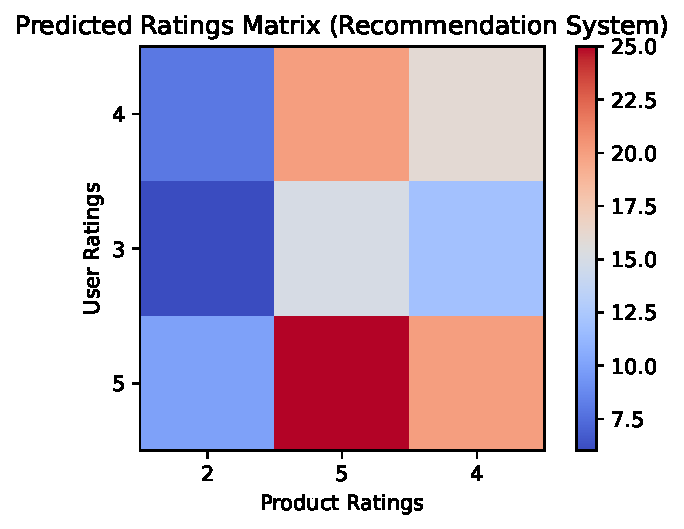
\includegraphics{module_2_files/figure-pdf/cell-29-output-3.pdf}

\begin{tcolorbox}[enhanced jigsaw, leftrule=.75mm, bottomtitle=1mm, colback=white, toptitle=1mm, opacitybacktitle=0.6, toprule=.15mm, colbacktitle=quarto-callout-note-color!10!white, arc=.35mm, colframe=quarto-callout-note-color-frame, title=\textcolor{quarto-callout-note-color}{\faInfo}\hspace{0.5em}{Additional Properties \& Definitions}, titlerule=0mm, rightrule=.15mm, left=2mm, bottomrule=.15mm, breakable, coltitle=black, opacityback=0]

\begin{enumerate}
\def\labelenumi{\arabic{enumi}.}
\item
  \textbf{Definition and Properties}

  Given two vectors:

  \begin{itemize}
  \tightlist
  \item
    \(\mathbf{u} \in \mathbb{R}^m\)
  \item
    \(\mathbf{v} \in \mathbb{R}^n\)
  \end{itemize}

  The outer product \(\mathbf{u} \otimes \mathbf{v}\) results in an
  \(m \times n\) matrix where each element \((i, j)\) of the matrix is
  calculated as:
  \[(\mathbf{u} \otimes \mathbf{v})_{ij} = u_i \cdot v_j\]
\item
  \textbf{Non-Symmetry}

  The outer product is generally not symmetric. For vectors
  \(\mathbf{u}\) and \(\mathbf{v}\), the matrix
  \(\mathbf{u} \otimes \mathbf{v}\) is not necessarily equal to
  \(\mathbf{v} \otimes \mathbf{u}\):
  \[\mathbf{u} \otimes \mathbf{v} \neq \mathbf{v} \otimes \mathbf{u}\]
\item
  \textbf{Rank of the Outer Product}

  The rank of the outer product matrix \(\mathbf{u} \otimes \mathbf{v}\)
  is always 1, provided neither \(\mathbf{u}\) nor \(\mathbf{v}\) is a
  zero vector. This is because the matrix can be expressed as a single
  rank-1 matrix.
\item
  \textbf{Distributive Property}

  The outer product is distributive over vector addition. For vectors
  \(\mathbf{u}_1, \mathbf{u}_2 \in \mathbb{R}^m\) and
  \(\mathbf{v} \in \mathbb{R}^n\):
  \[(\mathbf{u}_1 + \mathbf{u}_2) \otimes \mathbf{v} = (\mathbf{u}_1 \otimes \mathbf{v}) + (\mathbf{u}_2 \otimes \mathbf{v})\]
\item
  \textbf{Associativity with Scalar Multiplication}

  The outer product is associative with scalar multiplication. For a
  scalar \(\alpha\) and vectors \(\mathbf{u} \in \mathbb{R}^m\) and
  \(\mathbf{v} \in \mathbb{R}^n\):
  \[\alpha (\mathbf{u} \otimes \mathbf{v}) = (\alpha \mathbf{u}) \otimes \mathbf{v} = \mathbf{u} \otimes (\alpha \mathbf{v})\]
\item
  \textbf{Matrix Trace}

  The trace of the outer product of two vectors is given by:
  \[\text{tr}(\mathbf{u} \otimes \mathbf{v}) = (\mathbf{u}^T \mathbf{v})= (\mathbf{v}^T \mathbf{u})\]
  Here, \(\text{tr}\) denotes the trace of a matrix, which is the sum of
  its diagonal elements.
\item
  \textbf{Matrix Norm}

  The Frobenius norm of the outer product matrix can be expressed in
  terms of the norms of the original vectors:
  \[\| \mathbf{u} \otimes \mathbf{v} \|_F = \| \mathbf{u} \|_2 \cdot \| \mathbf{v} \|_2\]
  where \(\| \cdot \|_2\) denotes the Euclidean norm.
\end{enumerate}

\end{tcolorbox}

\textbf{Example Calculation in \texttt{Python}}

Here's how to compute and visualize the outer product properties using
\texttt{Python}:

\begin{Shaded}
\begin{Highlighting}[]
\ImportTok{import}\NormalTok{ numpy }\ImportTok{as}\NormalTok{ np}
\ImportTok{import}\NormalTok{ matplotlib.pyplot }\ImportTok{as}\NormalTok{ plt}

\CommentTok{\# Define vectors}
\NormalTok{u }\OperatorTok{=}\NormalTok{ np.array([}\DecValTok{1}\NormalTok{, }\DecValTok{2}\NormalTok{, }\DecValTok{3}\NormalTok{])}
\NormalTok{v }\OperatorTok{=}\NormalTok{ np.array([}\DecValTok{4}\NormalTok{, }\DecValTok{5}\NormalTok{])}

\CommentTok{\# Compute outer product}
\NormalTok{outer\_product }\OperatorTok{=}\NormalTok{ np.outer(u, v)}

\CommentTok{\# Display results}
\BuiltInTok{print}\NormalTok{(}\StringTok{"Outer Product Matrix:"}\NormalTok{)}
\BuiltInTok{print}\NormalTok{(outer\_product)}

\CommentTok{\# Compute and display rank}
\NormalTok{rank }\OperatorTok{=}\NormalTok{ np.linalg.matrix\_rank(outer\_product)}
\BuiltInTok{print}\NormalTok{(}\SpecialStringTok{f"Rank of Outer Product Matrix: }\SpecialCharTok{\{}\NormalTok{rank}\SpecialCharTok{\}}\SpecialStringTok{"}\NormalTok{)}

\CommentTok{\# Compute Frobenius norm}
\NormalTok{frobenius\_norm }\OperatorTok{=}\NormalTok{ np.linalg.norm(outer\_product, }\StringTok{\textquotesingle{}fro\textquotesingle{}}\NormalTok{)}
\BuiltInTok{print}\NormalTok{(}\SpecialStringTok{f"Frobenius Norm: }\SpecialCharTok{\{}\NormalTok{frobenius\_norm}\SpecialCharTok{\}}\SpecialStringTok{"}\NormalTok{)}

\CommentTok{\# Plot the result}
\NormalTok{plt.imshow(outer\_product, cmap}\OperatorTok{=}\StringTok{\textquotesingle{}viridis\textquotesingle{}}\NormalTok{, interpolation}\OperatorTok{=}\StringTok{\textquotesingle{}nearest\textquotesingle{}}\NormalTok{)}
\NormalTok{plt.colorbar()}
\NormalTok{plt.title(}\StringTok{\textquotesingle{}Outer Product Matrix\textquotesingle{}}\NormalTok{)}
\NormalTok{plt.xlabel(}\StringTok{\textquotesingle{}Vector v\textquotesingle{}}\NormalTok{)}
\NormalTok{plt.ylabel(}\StringTok{\textquotesingle{}Vector u\textquotesingle{}}\NormalTok{)}
\NormalTok{plt.xticks(ticks}\OperatorTok{=}\NormalTok{np.arange(}\BuiltInTok{len}\NormalTok{(v)), labels}\OperatorTok{=}\NormalTok{v)}
\NormalTok{plt.yticks(ticks}\OperatorTok{=}\NormalTok{np.arange(}\BuiltInTok{len}\NormalTok{(u)), labels}\OperatorTok{=}\NormalTok{u)}
\NormalTok{plt.show()}
\end{Highlighting}
\end{Shaded}

\begin{verbatim}
Outer Product Matrix:
[[ 4  5]
 [ 8 10]
 [12 15]]
Rank of Outer Product Matrix: 1
Frobenius Norm: 23.958297101421877
\end{verbatim}

\begin{figure}[H]

\centering{

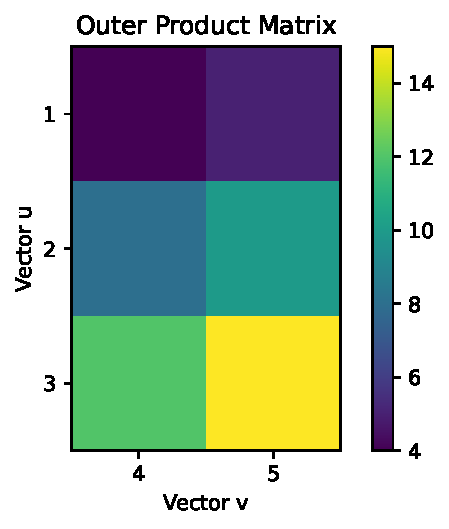
\includegraphics{module_2_files/figure-pdf/fig-op-output-2.pdf}

}

\caption{\label{fig-op}Demonstration of Outer Product and its
Properties}

\end{figure}%

\subsubsection*{Kronecker Product}\label{kronecker-product}
\addcontentsline{toc}{subsubsection}{Kronecker Product}

In mathematics, the Kronecker product, sometimes denoted by \(\otimes\),
is an operation on two matrices of arbitrary size resulting in a
\emph{block matrix}. It is a specialization of the tensor product (which
is denoted by the same symbol) from vectors to matrices and gives the
matrix of the tensor product linear map with respect to a standard
choice of basis. The Kronecker product is to be distinguished from the
usual matrix multiplication, which is an entirely different operation.
The Kronecker product is also sometimes called \emph{matrix direct
product}.

\begin{tcolorbox}[enhanced jigsaw, leftrule=.75mm, bottomtitle=1mm, colback=white, toptitle=1mm, opacitybacktitle=0.6, toprule=.15mm, colbacktitle=quarto-callout-note-color!10!white, arc=.35mm, colframe=quarto-callout-note-color-frame, title=\textcolor{quarto-callout-note-color}{\faInfo}\hspace{0.5em}{Note}, titlerule=0mm, rightrule=.15mm, left=2mm, bottomrule=.15mm, breakable, coltitle=black, opacityback=0]

If \(A\) is an \(m \times n\) matrix and \(B\) is a \(p \times q\)
matrix, then the Kronecker product \(A\otimes B\) is the
\(pm \times qn\) block matrix defined as: Each \(a_{ij}\) of \(A\) is
replaced by the matrix \(a_{ij}B\). Symbolically this will result in a
block matrix defined by:

\[A\otimes B=A \otimes B = \begin{bmatrix}a_{11}B & a_{12}B & \cdots & a_{1n}B \\a_{21}B & a_{22}B & \cdots & a_{2n}B \\\vdots & \vdots & \ddots & vdots \\a_{m1}B & a_{m2}B & \cdots & a_{mn}B\end{bmatrix}\]

\end{tcolorbox}

\begin{tcolorbox}[enhanced jigsaw, leftrule=.75mm, bottomtitle=1mm, colback=white, toptitle=1mm, opacitybacktitle=0.6, toprule=.15mm, colbacktitle=quarto-callout-note-color!10!white, arc=.35mm, colframe=quarto-callout-note-color-frame, title=\textcolor{quarto-callout-note-color}{\faInfo}\hspace{0.5em}{Properties of the Kronecker Product}, titlerule=0mm, rightrule=.15mm, left=2mm, bottomrule=.15mm, breakable, coltitle=black, opacityback=0]

\begin{enumerate}
\def\labelenumi{\arabic{enumi}.}
\item
  \textbf{Associativity}

  The Kronecker product is associative. For matrices
  \(A \in \mathbb{R}^{m \times n}\), \(B \in \mathbb{R}^{p \times q}\),
  and \(C \in \mathbb{R}^{r \times s}\):
  \[(A \otimes B) \otimes C = A \otimes (B \otimes C)\]
\item
  \textbf{Distributivity Over Addition}

  The Kronecker product distributes over matrix addition. For matrices
  \(A \in \mathbb{R}^{m \times n}\), \(B \in \mathbb{R}^{p \times q}\),
  and \(C \in \mathbb{R}^{p \times q}\):
  \[A \otimes (B + C) = (A \otimes B) + (A \otimes C)\]
\item
  \textbf{Mixed Product Property}

  The Kronecker product satisfies the mixed product property with the
  matrix product. For matrices \(A \in \mathbb{R}^{m \times n}\),
  \(B \in \mathbb{R}^{p \times q}\), \(C \in \mathbb{R}^{r \times s}\),
  and \(D \in \mathbb{R}^{r \times s}\):
  \[(A \otimes B) (C \otimes D) = (A C) \otimes (B D)\]
\item
  \textbf{Transpose}

  The transpose of the Kronecker product is given by:
  \[(A \otimes B)^T = A^T \otimes B^T\]
\item
  \textbf{Norm}

  The Frobenius norm of the Kronecker product can be computed as:
  \[\| A \otimes B \|_F = \| A \|_F \cdot \| B \|_F\] where
  \(\| \cdot \|_F\) denotes the Frobenius norm.
\end{enumerate}

\end{tcolorbox}

\begin{center}\rule{0.5\linewidth}{0.5pt}\end{center}

\begin{tcolorbox}[enhanced jigsaw, leftrule=.75mm, bottomtitle=1mm, colback=white, toptitle=1mm, opacitybacktitle=0.6, toprule=.15mm, colbacktitle=quarto-callout-tip-color!10!white, arc=.35mm, colframe=quarto-callout-tip-color-frame, title=\textcolor{quarto-callout-tip-color}{\faLightbulb}\hspace{0.5em}{Frobenius Norm}, titlerule=0mm, rightrule=.15mm, left=2mm, bottomrule=.15mm, breakable, coltitle=black, opacityback=0]

The Frobenius norm, also known as the Euclidean norm for matrices, is a
measure of a matrix's magnitude. It is defined as the square root of the
sum of the absolute squares of its elements. Mathematically, for a
matrix \(A\) with elements \(a_{ij}\), the Frobenius norm is given by:

\[\|A\|_F = \sqrt{\sum_{i,j} |a_{ij}|^2}\]

\end{tcolorbox}

Example 1: Calculation of Frobenius Norm

Consider the matrix \(A\):

\[A = \begin{bmatrix}1 & 2 \\3 & 4\end{bmatrix}\]

To compute the Frobenius norm:

\[\|A\|_F = \sqrt{1^2 + 2^2 + 3^2 + 4^2}= \sqrt{1 + 4 + 9 + 16}= \sqrt{30}\approx 5.48\]

Example 2: Frobenius Norm of a Sparse Matrix

Consider the sparse matrix \(B\):

\[B = \begin{bmatrix}0 & 0 & 0 \\0 & 5 & 0 \\0 & 0 & 0\end{bmatrix}\]

To compute the Frobenius norm:

\[\|B\|_F = \sqrt{0^2 + 0^2 + 0^2 + 5^2 + 0^2 + 0^2}= \sqrt{25}= 5\]

Example 3: Frobenius Norm in a Large Matrix

Consider the matrix \(C\) of size \$3 \times 3 \$:

\[C = \begin{bmatrix}1 & 2 & 3 \\4 & 5 & 6 \\7 & 8 & 9\end{bmatrix}\]

To compute the Frobenius norm:

\begin{align*}
\|C\|_F &= \sqrt{1^2 + 2^2 + 3^2 + 4^2 + 5^2 + 6^2 + 7^2 + 8^2 + 9^2}\\
&= \sqrt{1 + 4 + 9 + 16 + 25 + 36 + 49 + 64 + 81}\\
&= \sqrt{285}\\
&\approx 16.88
\end{align*}

\textbf{Applications of the Frobenius Norm}

\begin{itemize}
\item
  \emph{Application 1: Image Compression:} In image processing, the
  Frobenius norm can measure the difference between the original and
  compressed images, indicating how well the compression has preserved
  the original image quality.
\item
  \emph{Application 2: Matrix Factorization:} In numerical analysis,
  Frobenius norm is used to evaluate the error in matrix approximations,
  such as in Singular Value Decomposition (SVD). A lower Frobenius norm
  of the error indicates a better approximation.
\item
  \emph{Application 3: Error Measurement in Numerical Solutions:} In
  solving systems of linear equations, the Frobenius norm can be used to
  measure the error between the true solution and the computed solution,
  providing insight into the accuracy of numerical methods.
\end{itemize}

The \texttt{linalg} sub module of \texttt{NumPy} library can be used to
calculate various norms. Basically norm is the generalized form of
Euclidean distance.

\begin{Shaded}
\begin{Highlighting}[]
\ImportTok{import}\NormalTok{ numpy }\ImportTok{as}\NormalTok{ np}

\CommentTok{\# Example 1: Simple Matrix}
\NormalTok{A }\OperatorTok{=}\NormalTok{ np.array([[}\DecValTok{1}\NormalTok{, }\DecValTok{2}\NormalTok{], [}\DecValTok{3}\NormalTok{, }\DecValTok{4}\NormalTok{]])}
\NormalTok{frobenius\_norm\_A }\OperatorTok{=}\NormalTok{ np.linalg.norm(A, }\StringTok{\textquotesingle{}fro\textquotesingle{}}\NormalTok{)}
\BuiltInTok{print}\NormalTok{(}\SpecialStringTok{f"Frobenius Norm of A: }\SpecialCharTok{\{}\NormalTok{frobenius\_norm\_A}\SpecialCharTok{:.2f\}}\SpecialStringTok{"}\NormalTok{)}

\CommentTok{\# Example 2: Sparse Matrix}
\NormalTok{B }\OperatorTok{=}\NormalTok{ np.array([[}\DecValTok{0}\NormalTok{, }\DecValTok{0}\NormalTok{, }\DecValTok{0}\NormalTok{], [}\DecValTok{0}\NormalTok{, }\DecValTok{5}\NormalTok{, }\DecValTok{0}\NormalTok{], [}\DecValTok{0}\NormalTok{, }\DecValTok{0}\NormalTok{, }\DecValTok{0}\NormalTok{]])}
\NormalTok{frobenius\_norm\_B }\OperatorTok{=}\NormalTok{ np.linalg.norm(B, }\StringTok{\textquotesingle{}fro\textquotesingle{}}\NormalTok{)}
\BuiltInTok{print}\NormalTok{(}\SpecialStringTok{f"Frobenius Norm of B: }\SpecialCharTok{\{}\NormalTok{frobenius\_norm\_B}\SpecialCharTok{:.2f\}}\SpecialStringTok{"}\NormalTok{)}

\CommentTok{\# Example 3: Large Matrix}
\NormalTok{C }\OperatorTok{=}\NormalTok{ np.array([[}\DecValTok{1}\NormalTok{, }\DecValTok{2}\NormalTok{, }\DecValTok{3}\NormalTok{], [}\DecValTok{4}\NormalTok{, }\DecValTok{5}\NormalTok{, }\DecValTok{6}\NormalTok{], [}\DecValTok{7}\NormalTok{, }\DecValTok{8}\NormalTok{, }\DecValTok{9}\NormalTok{]])}
\NormalTok{frobenius\_norm\_C }\OperatorTok{=}\NormalTok{ np.linalg.norm(C, }\StringTok{\textquotesingle{}fro\textquotesingle{}}\NormalTok{)}
\BuiltInTok{print}\NormalTok{(}\SpecialStringTok{f"Frobenius Norm of C: }\SpecialCharTok{\{}\NormalTok{frobenius\_norm\_C}\SpecialCharTok{:.2f\}}\SpecialStringTok{"}\NormalTok{)}
\end{Highlighting}
\end{Shaded}

\begin{verbatim}
Frobenius Norm of A: 5.48
Frobenius Norm of B: 5.00
Frobenius Norm of C: 16.88
\end{verbatim}

\textbf{Frobenius norm of Kronecker product}

Let us consider two matrices,

\[A = \begin{bmatrix}1 & 2 \\3 & 4\end{bmatrix}\]

and

\[B = \begin{bmatrix}0 & 5 \\6 & 7\end{bmatrix}\]

The Kronecker product \(C = A \otimes B\) is:

\[C = \begin{bmatrix}1 \cdot B & 2 \cdot B \\3 \cdot B & 4 \cdot B\end{bmatrix}= \begin{bmatrix}\begin{bmatrix}0 & 5 \\6 & 7\end{bmatrix} & \begin{bmatrix}0 \cdot 2 & 5 \cdot 2 \\6 \cdot 2 & 7 \cdot 2\end{bmatrix} \\\begin{bmatrix}0 \cdot 3 & 5 \cdot 3 \\6 \cdot 3 & 7 \cdot 3\end{bmatrix} & \begin{bmatrix}0 \cdot 4 & 5 \cdot 4 \\6 \cdot 4 & 7 \cdot 4\end{bmatrix}\end{bmatrix}\]

This expands to:

\[C = \begin{bmatrix}0 & 5 & 0 & 10 \\6 & 7 & 12 & 14 \\0 & 15 & 0 & 20 \\18 & 21 & 24 & 28\end{bmatrix}\]

\emph{Computing the Frobenius Norm}

To compute the Frobenius norm of \(C\):

\[\|C\|_F = \sqrt{\sum_{i=1}^{4} \sum_{j=1}^{4} |c_{ij}|^2}\]

\[\|C\|_F = \sqrt{0^2 + 5^2 + 0^2 + 10^2 + 6^2 + 7^2 + 12^2 + 14^2 + 0^2 + 15^2 + 0^2 + 20^2 + 18^2 + 21^2 + 24^2 + 28^2}\]

\[\|C\|_F = \sqrt{0 + 25 + 0 + 100 + 36 + 49 + 144 + 196 + 0 + 225 + 0 + 400 + 324 + 441 + 576 + 784}\]

\[\|C\|_F = \sqrt{2896}\] \[\|C\|_F \approx 53.87\]

\begin{center}\rule{0.5\linewidth}{0.5pt}\end{center}

\subsubsection*{Practice Problems}\label{practice-problems-3}
\addcontentsline{toc}{subsubsection}{Practice Problems}

\textbf{Find the Kronecker product of A and B where A and B are given as
follows:}

\textbf{Problem 1:}

Find the Kronecker product of:
\[A=\begin{bmatrix}1&2\\3&4\end{bmatrix}\]
\[B=\begin{bmatrix}0&1\\1&0\end{bmatrix}\]

\textbf{Solution:}

\begin{align*}
A \otimes B &= \begin{bmatrix}1&2\\3&4\end{bmatrix} \otimes \begin{bmatrix}0&1\\1&0\end{bmatrix} \\
&= \begin{bmatrix}
1 \cdot \begin{bmatrix}0&1\\1&0\end{bmatrix} & 2 \cdot \begin{bmatrix}0&1\\1&0\end{bmatrix} \\
3 \cdot \begin{bmatrix}0&1\\1&0\end{bmatrix} & 4 \cdot \begin{bmatrix}0&1\\1&0\end{bmatrix}
\end{bmatrix} \\
&= \begin{bmatrix}
0 & 1 & 0 & 2 \\
1 & 0 & 2& 0\\
0 & 3 & 0 & 4 \\
3 & 0 & 4 & 0
\end{bmatrix}
\end{align*}

\begin{center}\rule{0.5\linewidth}{0.5pt}\end{center}

\textbf{Problem 2:}

Find the Kronecker product of:
\[A=\begin{bmatrix}1&0\\0&1\end{bmatrix}\]
\[B=\begin{bmatrix}2&3\\4&5\end{bmatrix}\]

\textbf{Solution:}

\begin{align*}
A \otimes B &= \begin{bmatrix}1&0\\0&1\end{bmatrix} \otimes \begin{bmatrix}2&3\\4&5\end{bmatrix} \\
&= \begin{bmatrix}
1 \cdot \begin{bmatrix}2&3\\4&5\end{bmatrix} & 0 \cdot \begin{bmatrix}2&3\\4&5\end{bmatrix} \\
0 \cdot \begin{bmatrix}2&3\\4&5\end{bmatrix} & 1 \cdot \begin{bmatrix}2&3\\4&5\end{bmatrix}
\end{bmatrix} \\
&= \begin{bmatrix}
2 & 3 & 0 & 0 \\
4 & 5 & 0 & 0 \\
0 & 0 & 2 & 3 \\
0 & 0 & 4 & 5
\end{bmatrix}
\end{align*}

\begin{center}\rule{0.5\linewidth}{0.5pt}\end{center}

\textbf{Problem 3:}

Find the Kronecker product of: \[A=\begin{bmatrix}1&2\end{bmatrix}\]
\[B=\begin{bmatrix}3\\4\end{bmatrix}\]

\textbf{Solution:}

\begin{align*}
A \otimes B &= \begin{bmatrix}1&2\end{bmatrix} \otimes \begin{bmatrix}3\\4\end{bmatrix} \\
&= \begin{bmatrix}
1 \cdot \begin{bmatrix}3\\4\end{bmatrix} & 2 \cdot \begin{bmatrix}3\\4\end{bmatrix}
\end{bmatrix} \\
&= \begin{bmatrix}
3 & 6 \\
4 & 8
\end{bmatrix}
\end{align*}

\begin{center}\rule{0.5\linewidth}{0.5pt}\end{center}

\textbf{Problem 4:}

Find the Kronecker product of: \[A=\begin{bmatrix}0&1\end{bmatrix}\]
\[B=\begin{bmatrix}1&-1\\2&0\end{bmatrix}\]

\textbf{Solution:}

\begin{align*}
A \otimes B &= \begin{bmatrix}0&1\end{bmatrix} \otimes \begin{bmatrix}1&-1\\2&0\end{bmatrix} \\
&= \begin{bmatrix}
0 \cdot \begin{bmatrix}1&-1\\2&0\end{bmatrix} & 1 \cdot \begin{bmatrix}1&-1\\2&0\end{bmatrix}
\end{bmatrix} \\
&= \begin{bmatrix}
0 & 0 &1&-1\\
0 & 0&2&0 \\
\end{bmatrix}
\end{align*}

\begin{center}\rule{0.5\linewidth}{0.5pt}\end{center}

\textbf{Problem 5:}

Find the Kronecker product of: \[A=\begin{bmatrix}2\\3\end{bmatrix}\]
\[B=\begin{bmatrix}4&-2\end{bmatrix}\]

\textbf{Solution:}

\begin{align*}
A \otimes B &= \begin{bmatrix}2\\3\end{bmatrix} \otimes \begin{bmatrix}4&-2\end{bmatrix} \\
&= \begin{bmatrix}
2 \cdot \begin{bmatrix}4&-2\end{bmatrix} \\
3 \cdot \begin{bmatrix}4&-2\end{bmatrix}
\end{bmatrix} \\
&= \begin{bmatrix}
8 & -4 \\
12 & -6
\end{bmatrix}
\end{align*}

\begin{center}\rule{0.5\linewidth}{0.5pt}\end{center}

\textbf{Problem 6:}

Find the Kronecker product of:
\[A=\begin{bmatrix}1&-1\\0&2\end{bmatrix}\]
\[B=\begin{bmatrix}0&1\\1&0\end{bmatrix}\]

\textbf{Solution:}

\begin{align*}
A \otimes B &= \begin{bmatrix}1&-1\\0&2\end{bmatrix} \otimes \begin{bmatrix}0&1\\1&0\end{bmatrix} \\
&= \begin{bmatrix}
1 \cdot \begin{bmatrix}0&1\\1&0\end{bmatrix} & -1 \cdot \begin{bmatrix}0&1\\1&0\end{bmatrix} \\
0 \cdot \begin{bmatrix}0&1\\1&0\end{bmatrix} & 2 \cdot \begin{bmatrix}0&1\\1&0\end{bmatrix}
\end{bmatrix} \\
&= \begin{bmatrix}
0 & 1 & 0 & -1 \\
1 & 0 & -1 & 0 \\
0 & 0 & 0 & 2 \\
0 & 0 & 2 & 0
\end{bmatrix}
\end{align*}

\begin{center}\rule{0.5\linewidth}{0.5pt}\end{center}

\textbf{Problem 7:}

Find the Kronecker product of: \[A=\begin{bmatrix}2\end{bmatrix}\]
\[B=\begin{bmatrix}3&4\\5&6\end{bmatrix}\]

\textbf{Solution:}

\begin{align*}
A \otimes B &= \begin{bmatrix}2\end{bmatrix} \otimes \begin{bmatrix}3&4\\5&6\end{bmatrix} \\
&= 2 \cdot \begin{bmatrix}3&4\\5&6\end{bmatrix} \\
&= \begin{bmatrix}
6 & 8 \\
10 & 12
\end{bmatrix}
\end{align*}

\begin{center}\rule{0.5\linewidth}{0.5pt}\end{center}

\textbf{Problem 8:}

Find the Kronecker product of: \[A=\begin{bmatrix}0&1\end{bmatrix}\]
\[B=\begin{bmatrix}1&0\\0&1\end{bmatrix}\]

\textbf{Solution:}

\begin{align*}
A \otimes B &= \begin{bmatrix}0&1\end{bmatrix} \otimes \begin{bmatrix}1&0\\0&1\end{bmatrix} \\
&= \begin{bmatrix}
0 \cdot \begin{bmatrix}1&0\\0&1\end{bmatrix} & 1 \cdot \begin{bmatrix}1&0\\0&1\end{bmatrix}
\end{bmatrix} \\
&= \begin{bmatrix}
0 & 0 \\
0 & 1
\end{bmatrix}
\end{align*}

\begin{center}\rule{0.5\linewidth}{0.5pt}\end{center}

\textbf{Problem 9:}

Find the Kronecker product of:
\[A=\begin{bmatrix}1&0\\0&1\end{bmatrix}\]
\[B=\begin{bmatrix}1&1\\1&1\end{bmatrix}\]

\textbf{Solution:}

\begin{align*}
A \otimes B &= \begin{bmatrix}1&0\\0&1\end{bmatrix} \otimes \begin{bmatrix}1&1\\1&1\end{bmatrix} \\
&= \begin{bmatrix}
1 \cdot \begin{bmatrix}1&1\\1&1\end{bmatrix} & 0 \cdot \begin{bmatrix}1&1\\1&1\end{bmatrix} \\
0 \cdot \begin{bmatrix}1&1\\1&1\end{bmatrix} & 1 \cdot \begin{bmatrix}1&1\\1&1\end{bmatrix}
\end{bmatrix} \\
&= \begin{bmatrix}
1 & 1 & 0 & 0 \\
1 & 1 & 0 & 0 \\
0 & 0 & 1 & 1 \\
0 & 0 & 1 & 1
\end{bmatrix}
\end{align*}

\begin{center}\rule{0.5\linewidth}{0.5pt}\end{center}

\textbf{Problem 10:}

Find the Kronecker product of:
\[A=\begin{bmatrix}2&-1\\3&4\end{bmatrix}\]
\[B=\begin{bmatrix}0&5\\-2&3\end{bmatrix}\]

\textbf{Solution:}

\begin{align*}
A \otimes B &= \begin{bmatrix}2&-1\\3&4\end{bmatrix} \otimes \begin{bmatrix}0&5\\-2&3\end{bmatrix} \\
&= \begin{bmatrix}
2 \cdot \begin{bmatrix}0&5\\-2&3\end{bmatrix} & -1 \cdot \begin{bmatrix}0&5\\-2&3\end{bmatrix} \\
3 \cdot \begin{bmatrix}0&5\\-2&3\end{bmatrix} & 4 \cdot \begin{bmatrix}0&5\\-2&3\end{bmatrix}
\end{bmatrix} \\
&= \begin{bmatrix}
0 & 10 & 0 & -5 \\
-4 & 6 & 2 & -3 \\
0 & 15 & 0 & 20 \\
-6 & 9 & -8 & 12
\end{bmatrix}
\end{align*}

\begin{center}\rule{0.5\linewidth}{0.5pt}\end{center}

\subsubsection*{Connection Between Outer Product and Kronecker
Product}\label{connection-between-outer-product-and-kronecker-product}
\addcontentsline{toc}{subsubsection}{Connection Between Outer Product
and Kronecker Product}

\begin{enumerate}
\def\labelenumi{\arabic{enumi}.}
\item
  \textbf{Conceptual Connection:}

  \begin{itemize}
  \item
    The \textbf{outer product} is a special case of the
    \textbf{Kronecker product}. Specifically, if \(\mathbf{A}\) is a
    column vector and \(\mathbf{B}\) is a row vector, then
    \(\mathbf{A}\) is a \(m \times 1\) matrix and \(\mathbf{B}\) is a
    \(1 \times n\) matrix. The Kronecker product of these two matrices
    will yield the same result as the outer product of these vectors.
  \item
    For matrices \(\mathbf{A}\) and \(\mathbf{B}\), the Kronecker
    product involves taking the outer product of each element of
    \(\mathbf{A}\) with the entire matrix \(\mathbf{B}\).
  \end{itemize}
\item
  \textbf{Mathematical Formulation:}

  \begin{itemize}
  \tightlist
  \item
    Let
    \(\mathbf{A} = \begin{bmatrix}a_{11} & a_{12}\\ a_{21} & a_{22}\end{bmatrix}\)
    and
    \(\mathbf{B} = \begin{bmatrix}b_{11} & b_{12}\\ b_{21} & b_{22}\end{bmatrix}\).
    Then:
  \end{itemize}

  \[\mathbf{A} \otimes \mathbf{B} = \begin{bmatrix} a_{11} \mathbf{B} & a_{12} \mathbf{B} \\ a_{21} \mathbf{B} & a_{22} \mathbf{B} \end{bmatrix}\]

  \begin{itemize}
  \tightlist
  \item
    If \(\mathbf{A} = \mathbf{u} \mathbf{v}^T\) where \(\mathbf{u}\) is
    a column vector and \(\mathbf{v}^T\) is a row vector, then the
    Kronecker product of \(\mathbf{u}\) and \(\mathbf{v}^T\) yields the
    same result as the outer product \(\mathbf{u} \otimes \mathbf{v}\).
  \end{itemize}
\end{enumerate}

\begin{tcolorbox}[enhanced jigsaw, leftrule=.75mm, bottomtitle=1mm, colback=white, toptitle=1mm, opacitybacktitle=0.6, toprule=.15mm, colbacktitle=quarto-callout-note-color!10!white, arc=.35mm, colframe=quarto-callout-note-color-frame, title=\textcolor{quarto-callout-note-color}{\faInfo}\hspace{0.5em}{Note}, titlerule=0mm, rightrule=.15mm, left=2mm, bottomrule=.15mm, breakable, coltitle=black, opacityback=0]

\textbf{Summary}

\begin{itemize}
\tightlist
\item
  The \textbf{outer product} is a specific case of the \textbf{Kronecker
  product} where one of the matrices is a vector (either row or column).
\item
  The \textbf{Kronecker product} generalizes the outer product to
  matrices and is more versatile in applications involving tensor
  products and higher-dimensional constructs.
\end{itemize}

\end{tcolorbox}

\subsubsection*{Matrix Multiplication as Kronecker
Product}\label{matrix-multiplication-as-kronecker-product}
\addcontentsline{toc}{subsubsection}{Matrix Multiplication as Kronecker
Product}

Given matrices \(\mathbf{A}\) and \(\mathbf{B}\), where: -
\(\mathbf{A}\) is an \(m \times n\) matrix - \(\mathbf{B}\) is an
\(n \times p\) matrix

The product \(\mathbf{C} = \mathbf{A} \mathbf{B}\) can be expressed
using Kronecker products as:

\[\mathbf{C} = \sum_{k=1}^n (\mathbf{A}_{:,k} \otimes \mathbf{B}_{k,:})\]

where: - \(\mathbf{A}_{:,k}\) denotes the \(k\)-th column of matrix
\(\mathbf{A}\) - \(\mathbf{B}_{k,:}\) denotes the \(k\)-th row of matrix
\(\mathbf{B}\)

\textbf{Example:}

Let:

\[\mathbf{A} = \begin{bmatrix}1 & 2 \\3 & 4\end{bmatrix}\]

and:

\[\mathbf{B} = \begin{bmatrix}0 & 1 \\1 & 0\end{bmatrix}\]

To find \(\mathbf{C} = \mathbf{A} \mathbf{B}\) using Kronecker products:

\begin{enumerate}
\def\labelenumi{\arabic{enumi}.}
\item
  \textbf{Compute the Kronecker Product of Columns of \(\mathbf{A}\) and
  Rows of \(\mathbf{B}\):}

  \begin{itemize}
  \item
    For column
    \(\mathbf{A}_{:,1} = \begin{bmatrix} 1 \\ 3 \end{bmatrix}\) and row
    \(\mathbf{B}_{1,:} = \begin{bmatrix} 0 & 1 \end{bmatrix}\):
    \[\mathbf{A}_{:,1} \otimes \mathbf{B}_{1,:} = \begin{bmatrix}     0 & 1 \\     0 & 3     \end{bmatrix}\]
  \item
    For column
    \(\mathbf{A}_{:,2} = \begin{bmatrix} 2 \\ 4 \end{bmatrix}\) and row
    \(\mathbf{B}_{2,:} = \begin{bmatrix} 1 & 0 \end{bmatrix}\):
    \[\mathbf{A}_{:,2} \otimes \mathbf{B}_{2,:} = \begin{bmatrix}2 & 0 \\ 4 & 0\end{bmatrix}\]
  \end{itemize}
\item
  \textbf{Sum the Kronecker Products:}

  \[\mathbf{C} = \begin{bmatrix}0 & 1 \\ 0 & 3\end{bmatrix} +\begin{bmatrix} 2 & 0 \\ 4 & 0 \end{bmatrix}  = \begin{bmatrix} 2 & 1 \\ 4 & 3\end{bmatrix}\]
\end{enumerate}

\begin{center}\rule{0.5\linewidth}{0.5pt}\end{center}

In the previous block we have discussed the Frobenius norm and its
applications. Now came back to the discussions on the Kronecker product.
The Kronecker product is particularly useful in scenarios where
interactions between different types of data need to be modeled
comprehensively. In recommendation systems, it allows us to integrate
user preferences with item relationships to improve recommendation
accuracy.

In addition to recommendation systems, Kronecker products are used in
various fields such as:

\begin{itemize}
\tightlist
\item
  Signal Processing: For modeling multi-dimensional signals.
\item
  Machine Learning: In building features for complex models.
\item
  Communication Systems: For modeling network interactions.
\end{itemize}

By understanding the Kronecker product and its applications, we can
extend it to solve complex problems and enhance systems across different
domains. To understand the practical use of Kronecker product in a
Machine Learning scenario let us consider the following problem
statement and its solution.

\begin{tcolorbox}[enhanced jigsaw, leftrule=.75mm, bottomtitle=1mm, colback=white, toptitle=1mm, opacitybacktitle=0.6, toprule=.15mm, colbacktitle=quarto-callout-note-color!10!white, arc=.35mm, colframe=quarto-callout-note-color-frame, title=\textcolor{quarto-callout-note-color}{\faInfo}\hspace{0.5em}{Problem statement}, titlerule=0mm, rightrule=.15mm, left=2mm, bottomrule=.15mm, breakable, coltitle=black, opacityback=0]

In the realm of recommendation systems, predicting user preferences for
various product categories based on past interactions is a common
challenge. Suppose we have data on user preferences for different
products and categories. We can use this data to recommend the best
products for each user by employing mathematical tools such as the
Kronecker product. The User Preference and Category relationships are
given in Table~\ref{tbl-UPM} and Table~\ref{tbl-CRM} .

\begin{longtable}[]{@{}llll@{}}
\caption{User Preference}\label{tbl-UPM}\tabularnewline
\toprule\noalign{}
User/Item & Electronics & Clothing & Books \\
\midrule\noalign{}
\endfirsthead
\toprule\noalign{}
User/Item & Electronics & Clothing & Books \\
\midrule\noalign{}
\endhead
\bottomrule\noalign{}
\endlastfoot
User 1 & 5 & 3 & 4 \\
User 2 & 2 & 4 & 5 \\
User 3 & 3 & 4 & 4 \\
\end{longtable}

\begin{longtable}[]{@{}llll@{}}
\caption{Category Relationships}\label{tbl-CRM}\tabularnewline
\toprule\noalign{}
Category/Feature & Feature 1 & Feature 2 & Feature 3 \\
\midrule\noalign{}
\endfirsthead
\toprule\noalign{}
Category/Feature & Feature 1 & Feature 2 & Feature 3 \\
\midrule\noalign{}
\endhead
\bottomrule\noalign{}
\endlastfoot
Electronics & 1 & 0 & 0 \\
Clothing & 0 & 1 & 1 \\
Books & 0 & 1 & 1 \\
\end{longtable}

Predict user preferences for different product categories using the
Kronecker product matrix.

\end{tcolorbox}

\begin{quote}
\textbf{Solution Procedure}
\end{quote}

\begin{enumerate}
\def\labelenumi{\arabic{enumi}.}
\item
  \emph{Compute the Kronecker Product:} Calculate the Kronecker product
  of matrices \(U\) and \(C\) to obtain matrix \(K\).

  To model the problem, we use the Kronecker product of the user
  preference matrix \(U\) and the category relationships matrix \(C\).
  This product allows us to predict the user's rating for each category
  by combining their preferences with the category features.
\end{enumerate}

\emph{Formulating Matrices}

User Preference Matrix (U): - Dimension: \(3\times 3\) (3 users, 3
items) - from the User preference data, we can create the User
Preference Matrix as follows:

\[U = \begin{pmatrix}5 & 3 & 4 \\2 & 4 & 5 \\3 & 4 & 4 \end{pmatrix}\]

Category Relationships Matrix (C): - Dimension: \(3 \times 3\) (3
categories) - from the Category Relationships data, we can create the
Category Relationship Matrix as follows:

\[C = \begin{pmatrix}1 & 0 & 0 \\ 0 & 1 & 1 \\ 0 & 1 & 1\end{pmatrix}\]

\emph{Kronecker Product Calculation}

The Kronecker product \(K\) of \(U\) and \(C\) is calculated as follows:

\begin{enumerate}
\def\labelenumi{\arabic{enumi}.}
\tightlist
\item
  \textbf{Matrix Dimensions:}
\end{enumerate}

\begin{itemize}
\tightlist
\item
  \(U\) is \(3 \times 3\) (3 users, 3 items).
\item
  \(C\) is \(3 \times 3\) (3 categories, 3 features).
\end{itemize}

\begin{enumerate}
\def\labelenumi{\arabic{enumi}.}
\setcounter{enumi}{1}
\tightlist
\item
  \textbf{Calculate Kronecker Product:}
\end{enumerate}

\begin{itemize}
\tightlist
\item
  For each element \(u_{ij}\) in \(U\), multiply by the entire matrix
  \(C\).
\end{itemize}

The Kronecker product \(K\) is computed as:

\[K = U \otimes C\]

Explicitly, the Kronecker product \(K\) is:

\[K = \begin{pmatrix}5 \cdot C & 3 \cdot C & 4 \cdot C \\ 2 \cdot C & 4 \cdot C & 5 \cdot C \\    3 \cdot C & 4 \cdot C & 4 \cdot C\end{pmatrix}\]

As an example the blocks in first row are:

\[5 \cdot C = \begin{pmatrix}   5 & 0 & 0 \\   0 & 5 & 5 \\   0 & 5 & 5   \end{pmatrix}, \quad    3 \cdot C = \begin{pmatrix}   3 & 0 & 0 \\   0 & 3 & 3 \\   0 & 3 & 3   \end{pmatrix}, \quad   4 \cdot C = \begin{pmatrix}   4 & 0 & 0 \\   0 & 4 & 4 \\   0 & 4 & 4   \end{pmatrix}\]

Combining these blocks:

\[K = \begin{pmatrix}   5 & 0 & 0 & 3 & 0 & 0 & 4 & 0 & 0\\   0 & 5 & 5 & 0 & 3 & 3 & 0 & 4 & 4\\   0 & 5 & 5 & 0 & 3 & 3 & 0 & 4 & 4\\   2 & 0 & 0 & 4 & 0 & 0 & 5 & 0 & 0\\   0 & 2 & 2 & 0 & 4 & 4 & 0 & 5 & 5\\   0 & 2 & 2 & 0 & 4 & 4 & 0 & 5 & 5\\   3 & 0 & 0 & 4 & 0 & 0 & 4 & 0 & 0\\   0 & 3 & 3 & 0 & 4 & 4 & 0 & 4 & 4\\   0 & 3 & 3 & 0 & 4 & 4 & 0 & 4 & 4\end{pmatrix}\]

\begin{enumerate}
\def\labelenumi{\arabic{enumi}.}
\setcounter{enumi}{1}
\item
  \textbf{Interpret the Kronecker Product Matrix:} The resulting matrix
  \(K\) represents all possible combinations of user preferences and
  category features.
\item
  \textbf{Predict Ratings:} For each user, use matrix \(K\) to predict
  the rating for each category by summing up the values in the
  corresponding rows.
\item
  \textbf{Generate Recommendations:} Identify the top categories with
  the highest predicted ratings for each user.
\end{enumerate}

The \texttt{python} code to solve this problem computationally is given
below.

\begin{Shaded}
\begin{Highlighting}[]
\ImportTok{import}\NormalTok{ numpy }\ImportTok{as}\NormalTok{ np}
\ImportTok{import}\NormalTok{ pandas }\ImportTok{as}\NormalTok{ pd}
\ImportTok{import}\NormalTok{ matplotlib.pyplot }\ImportTok{as}\NormalTok{ plt}

\CommentTok{\# Define the matrices}
\NormalTok{U }\OperatorTok{=}\NormalTok{ np.array([[}\DecValTok{5}\NormalTok{, }\DecValTok{3}\NormalTok{, }\DecValTok{4}\NormalTok{],}
\NormalTok{              [}\DecValTok{2}\NormalTok{, }\DecValTok{4}\NormalTok{, }\DecValTok{5}\NormalTok{],}
\NormalTok{              [}\DecValTok{3}\NormalTok{, }\DecValTok{4}\NormalTok{, }\DecValTok{4}\NormalTok{]])}

\NormalTok{C }\OperatorTok{=}\NormalTok{ np.array([[}\DecValTok{1}\NormalTok{, }\DecValTok{0}\NormalTok{, }\DecValTok{0}\NormalTok{],}
\NormalTok{              [}\DecValTok{0}\NormalTok{, }\DecValTok{1}\NormalTok{, }\DecValTok{1}\NormalTok{],}
\NormalTok{              [}\DecValTok{0}\NormalTok{, }\DecValTok{1}\NormalTok{, }\DecValTok{1}\NormalTok{]])}

\CommentTok{\# Compute the Kronecker product}
\NormalTok{K }\OperatorTok{=}\NormalTok{ np.kron(U, C)}

\CommentTok{\# Create a DataFrame to visualize the Kronecker product matrix}
\NormalTok{df\_K }\OperatorTok{=}\NormalTok{ pd.DataFrame(K, }
\NormalTok{                    columns}\OperatorTok{=}\NormalTok{[}\StringTok{\textquotesingle{}Electronics\_F1\textquotesingle{}}\NormalTok{, }\StringTok{\textquotesingle{}Electronics\_F2\textquotesingle{}}\NormalTok{, }\StringTok{\textquotesingle{}Electronics\_F3\textquotesingle{}}\NormalTok{, }
                             \StringTok{\textquotesingle{}Clothing\_F1\textquotesingle{}}\NormalTok{, }\StringTok{\textquotesingle{}Clothing\_F2\textquotesingle{}}\NormalTok{, }\StringTok{\textquotesingle{}Clothing\_F3\textquotesingle{}}\NormalTok{, }
                             \StringTok{\textquotesingle{}Books\_F1\textquotesingle{}}\NormalTok{, }\StringTok{\textquotesingle{}Books\_F2\textquotesingle{}}\NormalTok{, }\StringTok{\textquotesingle{}Books\_F3\textquotesingle{}}\NormalTok{],}
\NormalTok{                    index}\OperatorTok{=}\NormalTok{[}\StringTok{\textquotesingle{}User 1 Electronics\textquotesingle{}}\NormalTok{, }\StringTok{\textquotesingle{}User 1 Clothing\textquotesingle{}}\NormalTok{, }\StringTok{\textquotesingle{}User 1 Books\textquotesingle{}}\NormalTok{, }
                           \StringTok{\textquotesingle{}User 2 Electronics\textquotesingle{}}\NormalTok{, }\StringTok{\textquotesingle{}User 2 Clothing\textquotesingle{}}\NormalTok{, }\StringTok{\textquotesingle{}User 2 Books\textquotesingle{}}\NormalTok{, }
                           \StringTok{\textquotesingle{}User 3 Electronics\textquotesingle{}}\NormalTok{, }\StringTok{\textquotesingle{}User 3 Clothing\textquotesingle{}}\NormalTok{, }\StringTok{\textquotesingle{}User 3 Books\textquotesingle{}}\NormalTok{])}

\CommentTok{\# Print the Kronecker product matrix}
\BuiltInTok{print}\NormalTok{(}\StringTok{"Kronecker Product Matrix (K):}\CharTok{\textbackslash{}n}\StringTok{"}\NormalTok{, df\_K)}

\CommentTok{\# Predict ratings and create recommendations}
\KeywordTok{def}\NormalTok{ recommend(user\_index, top\_n}\OperatorTok{=}\DecValTok{3}\NormalTok{):}
    \CommentTok{""" Recommend top\_n categories for a given user based on Kronecker product matrix. """}
\NormalTok{    user\_ratings }\OperatorTok{=}\NormalTok{ K[user\_index }\OperatorTok{*} \BuiltInTok{len}\NormalTok{(C):(user\_index }\OperatorTok{+} \DecValTok{1}\NormalTok{) }\OperatorTok{*} \BuiltInTok{len}\NormalTok{(C), :]}
\NormalTok{    predicted\_ratings }\OperatorTok{=}\NormalTok{ np.}\BuiltInTok{sum}\NormalTok{(user\_ratings, axis}\OperatorTok{=}\DecValTok{0}\NormalTok{)}
\NormalTok{    recommendations }\OperatorTok{=}\NormalTok{ np.argsort(predicted\_ratings)[::}\OperatorTok{{-}}\DecValTok{1}\NormalTok{][:top\_n]}
    \ControlFlowTok{return}\NormalTok{ recommendations}

\CommentTok{\# Recommendations for User 1}
\NormalTok{user\_index }\OperatorTok{=} \DecValTok{0}  \CommentTok{\# User 1}
\NormalTok{top\_n }\OperatorTok{=} \DecValTok{3}
\NormalTok{recommendations }\OperatorTok{=}\NormalTok{ recommend(user\_index, top\_n)}

\BuiltInTok{print}\NormalTok{(}\SpecialStringTok{f"}\CharTok{\textbackslash{}n}\SpecialStringTok{Top }\SpecialCharTok{\{}\NormalTok{top\_n}\SpecialCharTok{\}}\SpecialStringTok{ recommendations for User }\SpecialCharTok{\{}\NormalTok{user\_index }\OperatorTok{+} \DecValTok{1}\SpecialCharTok{\}}\SpecialStringTok{:"}\NormalTok{)}
\ControlFlowTok{for}\NormalTok{ rec }\KeywordTok{in}\NormalTok{ recommendations:}
    \BuiltInTok{print}\NormalTok{(df\_K.columns[rec])}
\end{Highlighting}
\end{Shaded}

\begin{verbatim}
Kronecker Product Matrix (K):
                     Electronics_F1  Electronics_F2  Electronics_F3  \
User 1 Electronics               5               0               0   
User 1 Clothing                  0               5               5   
User 1 Books                     0               5               5   
User 2 Electronics               2               0               0   
User 2 Clothing                  0               2               2   
User 2 Books                     0               2               2   
User 3 Electronics               3               0               0   
User 3 Clothing                  0               3               3   
User 3 Books                     0               3               3   

                    Clothing_F1  Clothing_F2  Clothing_F3  Books_F1  Books_F2  \
User 1 Electronics            3            0            0         4         0   
User 1 Clothing               0            3            3         0         4   
User 1 Books                  0            3            3         0         4   
User 2 Electronics            4            0            0         5         0   
User 2 Clothing               0            4            4         0         5   
User 2 Books                  0            4            4         0         5   
User 3 Electronics            4            0            0         4         0   
User 3 Clothing               0            4            4         0         4   
User 3 Books                  0            4            4         0         4   

                    Books_F3  
User 1 Electronics         0  
User 1 Clothing            4  
User 1 Books               4  
User 2 Electronics         0  
User 2 Clothing            5  
User 2 Books               5  
User 3 Electronics         0  
User 3 Clothing            4  
User 3 Books               4  

Top 3 recommendations for User 1:
Electronics_F2
Electronics_F3
Books_F3
\end{verbatim}

A simple visualization of this recomendation system is shown in
Fig~\ref{fig-reco}.

\begin{Shaded}
\begin{Highlighting}[]
\CommentTok{\# Visualization}
\KeywordTok{def}\NormalTok{ plot\_recommendations(user\_index):}
    \CommentTok{""" Plot the predicted ratings for each category for a given user. """}
\NormalTok{    user\_ratings }\OperatorTok{=}\NormalTok{ K[user\_index }\OperatorTok{*} \BuiltInTok{len}\NormalTok{(C):(user\_index }\OperatorTok{+} \DecValTok{1}\NormalTok{) }\OperatorTok{*} \BuiltInTok{len}\NormalTok{(C), :]}
\NormalTok{    predicted\_ratings }\OperatorTok{=}\NormalTok{ np.}\BuiltInTok{sum}\NormalTok{(user\_ratings, axis}\OperatorTok{=}\DecValTok{0}\NormalTok{)}
\NormalTok{    categories }\OperatorTok{=}\NormalTok{ df\_K.columns}
\NormalTok{    plt.figure(figsize}\OperatorTok{=}\NormalTok{(}\DecValTok{6}\NormalTok{, }\DecValTok{5}\NormalTok{))}
\NormalTok{    plt.bar(categories, predicted\_ratings)}
\NormalTok{    plt.xlabel(}\StringTok{\textquotesingle{}Categories\textquotesingle{}}\NormalTok{)}
\NormalTok{    plt.ylabel(}\StringTok{\textquotesingle{}Predicted Ratings\textquotesingle{}}\NormalTok{)}
\NormalTok{    plt.title(}\SpecialStringTok{f\textquotesingle{}Predicted Ratings for User }\SpecialCharTok{\{}\NormalTok{user\_index }\OperatorTok{+} \DecValTok{1}\SpecialCharTok{\}}\SpecialStringTok{\textquotesingle{}}\NormalTok{)}
\NormalTok{    plt.xticks(rotation}\OperatorTok{=}\DecValTok{45}\NormalTok{)}
\NormalTok{    plt.show()}

\CommentTok{\# Plot recommendations for User 1}
\NormalTok{plot\_recommendations(user\_index)}
\end{Highlighting}
\end{Shaded}

\begin{figure}[H]

\centering{

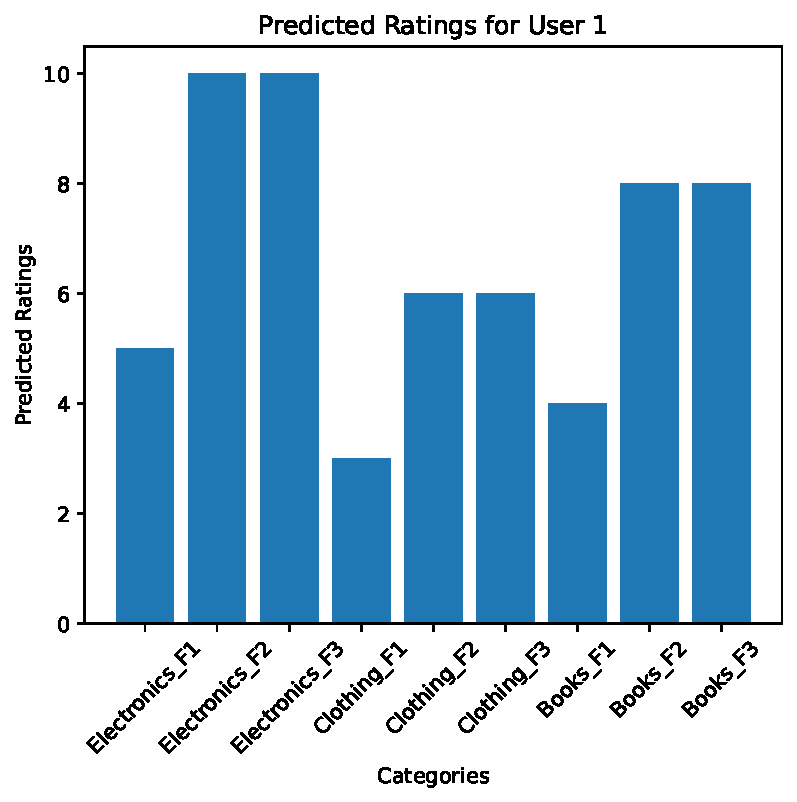
\includegraphics{module_2_files/figure-pdf/fig-reco-output-1.pdf}

}

\caption{\label{fig-reco}EDA for the Recommendation System}

\end{figure}%

This micro project illustrate one of the popular use of Kronecker
product on ML application.

\subsection*{Matrix Measures of Practical
Importance}\label{matrix-measures-of-practical-importance}
\addcontentsline{toc}{subsection}{Matrix Measures of Practical
Importance}

Matrix measures, such as rank and determinant, play crucial roles in
linear algebra. While both rank and determinant provide valuable
insights into the properties of a matrix, they serve different purposes.
Understanding their roles and applications is essential for solving
complex problems in computer science, engineering, and applied
mathematics.

\subsubsection*{Determinant}\label{determinant}
\addcontentsline{toc}{subsubsection}{Determinant}

Determinant of a \(2\times 2\) matrix
\(A=\begin{pmatrix}a&b\\c&d\end{pmatrix}\) is defined as \(|A|=ad-bc\).
Determinant of higher order square matrices can be found using the
Laplace method or Sarrus method.

The determinant of a matrix provides information about the matrix's
invertibility and scaling factor for volume transformation.
Specifically:

\begin{enumerate}
\def\labelenumi{\arabic{enumi}.}
\item
  \emph{Invertibility:} A matrix is invertible if and only if its
  determinant is non-zero.
\item
  \emph{Volume Scaling:} The absolute value of the determinant gives the
  scaling factor by which the matrix transforms volume.
\item
  \emph{Parallelism:} If the determinant of a matrix composed of vectors
  is zero, the vectors are linearly dependent, meaning they are parallel
  or redundant.
\item
  \emph{Redundancy:} A zero determinant indicates that the vectors span
  a space of lower dimension than the number of vectors, showing
  redundancy.
\end{enumerate}

\begin{tcolorbox}[enhanced jigsaw, leftrule=.75mm, bottomtitle=1mm, colback=white, toptitle=1mm, opacitybacktitle=0.6, toprule=.15mm, colbacktitle=quarto-callout-important-color!10!white, arc=.35mm, colframe=quarto-callout-important-color-frame, title=\textcolor{quarto-callout-important-color}{\faExclamation}\hspace{0.5em}{Least Possible Values of Determinant}, titlerule=0mm, rightrule=.15mm, left=2mm, bottomrule=.15mm, breakable, coltitle=black, opacityback=0]

\begin{enumerate}
\def\labelenumi{\arabic{enumi}.}
\tightlist
\item
  \emph{Least Positive Determinant:} For a \(1\times 1\) matrix, the
  smallest non-zero determinant is any positive value, typically
  \(\epsilon\), where \(\epsilon\) is a small positive number.
\item
  Least Non-Zero Determinant: For higher-dimensional matrices, the
  smallest non-zero determinant is a non-zero value that represents the
  smallest area or volume spanned by the matrix's rows or columns. For
  example a \(2\times 2\) matrix with determinant \(\epsilon\) could be:
  \[B=\begin{pmatrix}\epsilon&0\\ 0&\epsilon\end{pmatrix}\] Here,
  \(\epsilon\) is a small positive number, indicating a very small but
  \emph{non-zero} area.
\end{enumerate}

\end{tcolorbox}

Now let's look into the most important matrix measure for advanced
application in Linear Algebra.

As we know the matrix is basically a representation tool that make
things abstract- remove unnecessary details. Then the matrix itself can
be represented in many ways. This is the real story telling with this
most promising mathematical structure. Consider a context of collecting
feedback about a product in three aspects- cost, quality and
practicality. For simplicity in calculation, we consider responses from
3 customers only. The data is shown in Table~\ref{tbl-RT}.

\begin{longtable}[]{@{}llll@{}}
\caption{User rating of a consumer product}\label{tbl-RT}\tabularnewline
\toprule\noalign{}
User & Cost & Quality & Practicality \\
\midrule\noalign{}
\endfirsthead
\toprule\noalign{}
User & Cost & Quality & Practicality \\
\midrule\noalign{}
\endhead
\bottomrule\noalign{}
\endlastfoot
User-1 & 1 & 4 & 5 \\
User-2 & 3 & 2 & 5 \\
User-3 & 2 & 1 & 3 \\
\end{longtable}

It's perfect and nice looking. But both mathematics and a computer can't
handle this table as it is. So we create an abstract representation of
this data- the rating matrix. Using the traditional approach, let's
represent this rating data as:
\[A=\begin{bmatrix}1&4&5\\3&2&5\\2&1&3\end{bmatrix}\]

Now both the column names and row indices were removed and the data is
transformed into the abstract form. This representation has both
advantages and disadvantages. Be positive! So we are focused only in the
advantages.

Just consider the product. Its sales fully based on its features. So the
product sales perspective will be represented in terms of the features-
cost, quality and practicality. These features are columns of our rating
matrix. Definitly people will have different rating for these features.
Keeping all these in mind let's introduce the concept of \emph{linear
combination}. This leads to a new matrix product as shown below.

\begin{align*}
Ax&=\begin{bmatrix}
1&4&5\\
3&2&5\\
2&1&3
\end{bmatrix}x\\
&=\begin{bmatrix}
1&4&5\\
3&2&5\\
2&1&3
\end{bmatrix}\cdot\begin{bmatrix}x_1\\x_2\\x_3\end{bmatrix}\\
&=\begin{bmatrix}1\\3\\2\end{bmatrix}x_1+\begin{bmatrix}4\\2\\1\end{bmatrix}x_2+\begin{bmatrix}5\\5\\3\end{bmatrix}x_3
\end{align*}

As the number of users increases, the product sales perspective become
more informative. In short the span of the features define the feature
space of the product. In real cases, a manufacture wants to know what
are the features really inflence the customers. This new matrix product
will help the manufactures to identify that features!

So we are going to define this new matrix product as the feature space,
that will provide more insights to this context as:

\[A=CR\]

Where \(C\) is the column space and \(R\) is the row reduced Echelon
form of \(A\). But the product is not the usual scalar projection,
Instead the weight of linear combination of elements in the column
space.

Let's formally illustrate this in our example. From the first
observation itself, it is clear that last column is just the sum of
first and second columns (That is in our context the feature
`practicality' is just depends on `cost' and `quality'. meaningful?). So
only first columns are independent and so spans the column space.

\[C=\begin{bmatrix}1&4\\3&2\\2&1\end{bmatrix}\]

Now look into the matrix \(R\). Applying elementary row tansformations,
\(A\) will transformed into:

\[R=\begin{bmatrix}1&0&1\\0&1&1\\0&0&0\end{bmatrix}\]

Hence we can form a decomposition for the given rating matrix, \(A\) as:
\begin{align*}
A&=CR\\
&=\begin{bmatrix}1&4\\3&2\\2&1\end{bmatrix}\begin{bmatrix}1&0&1\\0&1&1\\\mbox{}&&\end{bmatrix}
\end{align*}

This decomposition says that there are only two independent features
(columns) and the third feature (column) is the sum of first two
features (columns).

\begin{tcolorbox}[enhanced jigsaw, leftrule=.75mm, bottomtitle=1mm, colback=white, toptitle=1mm, opacitybacktitle=0.6, toprule=.15mm, colbacktitle=quarto-callout-important-color!10!white, arc=.35mm, colframe=quarto-callout-important-color-frame, title=\textcolor{quarto-callout-important-color}{\faExclamation}\hspace{0.5em}{Interpretation of the \(R\) matrix}, titlerule=0mm, rightrule=.15mm, left=2mm, bottomrule=.15mm, breakable, coltitle=black, opacityback=0]

Each column in the \(R\) matrix represents the weights for linear
combination of vectors in the column space to get that column in \(A\).
In this example, third column of \(R\) is
\(\begin{bmatrix}1\\1\end{bmatrix}\). This means that third column of
\(A\) will be \(1\times C_1+1\times C_2\) of the column space, \(C\)!

\end{tcolorbox}

This first matrix decompostion donate a new type of matrix product
(outer product) and a new measure- the number of independent columns and
number of independent rows. This count is called the \emph{rank} of the
matrix \(A\). In the case of features, if the rank of the column space
is less than the number of features then definitly a less number of
feature set will perfectly represent the data. This will help us to
reduce the dimension of the dataset and there by reducing computational
complexities in data analysis and machine Learning jobs.

In the above discussion, we consider only the columns of \(A\). Now we
will mention the row space. It is the set of all linearly independent
rows of \(A\). For any matrix \(A\), both the row space and column space
are of same rank. This correspondance is a helpful result in many
practical applications.

Now we consider a stable equation, \(Ax=0\). With the usual notation of
dot product, it implies that \(x\) is orthogonal to \(A\). Set of all
those independent vectors which are orthogonal to \(A\) constitute a new
space of interest. It is called the \emph{null space} of \(A\). If \(A\)
represents a linear transformation, then the null space will be
populated by those non-zero vectors which are \emph{nullified} by the
transformation \(A\). As a summary of this discussion, the row space and
null space of a matrix \(A\) creates an orthogonal system. Considering
the relationship between \(A\) and \(A^T\), it is clear that row space
of \(A\) is same as the column space of \(A^T\) and vice verse are. So
we can restate the orthogonality as: `the null space of \(A\) is
orthogonal to the column space of \(A^T\)' and `the null space of
\(A^T\) is orthogonal to the column space of \(A\)'. Mathematically this
property can be represents as follows.

\begin{tcolorbox}[enhanced jigsaw, leftrule=.75mm, bottomtitle=1mm, colback=white, toptitle=1mm, opacitybacktitle=0.6, toprule=.15mm, colbacktitle=quarto-callout-note-color!10!white, arc=.35mm, colframe=quarto-callout-note-color-frame, title=\textcolor{quarto-callout-note-color}{\faInfo}\hspace{0.5em}{Note}, titlerule=0mm, rightrule=.15mm, left=2mm, bottomrule=.15mm, breakable, coltitle=black, opacityback=0]

\begin{align*}
\mathcal{N}(A)&\perp \mathcal{C}(A^T)\\
\mathcal{N}(A^T)&\perp \mathcal{C}(A)
\end{align*}

\end{tcolorbox}

In the given example, solving \(Ax=0\) we get
\(x=\begin{bmatrix}1&1&-1\end{bmatrix}^T\).

So the rank of \(\mathcal{N}(A)=1\). Already we have rank of \(A=2\).
This leads to an interesting result:

\[\text{Rank}(A)+\text{Rank}(\mathcal{N}(A))=3\]

This observation can be framed as a theorem.

\subsection*{Rank Nullity Theorem}\label{rank-nullity-theorem}
\addcontentsline{toc}{subsection}{Rank Nullity Theorem}

The rank-nullity theorem is a fundamental theorem in linear algebra that
is important for understanding the connections between mathematical
operations in engineering, physics, and computer science. It states that
the sum of the rank and nullity of a matrix equals the number of columns
in the matrix. The rank is the maximum number of linearly independent
columns, and the nullity is the dimension of the nullspace.

\begin{theorem}[Rank Nullitty
Theorem]\protect\hypertarget{thm-RNT}{}\label{thm-RNT}

The Rank-Nullity Theorem states that for any \(m \times n\) matrix
\(A\), the following relationship holds:

\[
\text{Rank}(A) + \text{Nullity}(A) = n
\]

where: - \textbf{Rank} of \(A\) is the dimension of the column space of
\(A\), which is also equal to the dimension of the row space of \(A\). -
\textbf{Nullity} of \(A\) is the dimension of the null space of \(A\),
which is the solution space to the homogeneous system
\(A \mathbf{x} = \mathbf{0}\).

\end{theorem}

\emph{Steps to Formulate for Matrix \(A\)}

\begin{enumerate}
\def\labelenumi{\arabic{enumi}.}
\item
  \textbf{Find the Rank of \(A\)}: The rank of a matrix is the maximum
  number of linearly independent columns (or rows). It can be determined
  by transforming \(A\) into its row echelon form or reduced row echelon
  form (RREF).
\item
  \textbf{Find the Nullity of \(A\)}: The nullity is the dimension of
  the solution space of \(A \mathbf{x} = \mathbf{0}\). This can be found
  by solving the homogeneous system and counting the number of free
  variables.
\item
  \textbf{Apply the Rank-Nullity Theorem}: Use the rank-nullity theorem
  to verify the relationship.
\end{enumerate}

\begin{center}\rule{0.5\linewidth}{0.5pt}\end{center}

\emph{Example 1:} Calculate the rank and nullity of
\(A=\begin{bmatrix}   1 & 4 & 5 \\   3 & 2 & 5 \\   2 & 1 & 3   \end{bmatrix}\)
and verify the rank nullity theorem.

\begin{enumerate}
\def\labelenumi{\arabic{enumi}.}
\item
  \textbf{Row Echelon Form}:

  Perform Gaussian elimination on \(A\):

  \[A = \begin{bmatrix} 1 & 4 & 5 \\  3 & 2 & 5 \\   2 & 1 & 3   \end{bmatrix}\]

  Perform row operations to get it to row echelon form:

  \begin{itemize}
  \item
    Subtract 3 times row 1 from row 2:
    \[\begin{bmatrix}     1 & 4 & 5 \\     0 & -10 & -10 \\     2 & 1 & 3     \end{bmatrix}\]
  \item
    Subtract 2 times row 1 from row 3:
    \[\begin{bmatrix}     1 & 4 & 5 \\     0 & -10 & -10 \\     0 & -7 & -7     \end{bmatrix}\]
  \item
    Add \(\frac{7}{10}\) times row 2 to row 3:
    \[\begin{bmatrix}     1 & 4 & 5 \\     0 & -10 & -10 \\     0 & 0 & 0     \end{bmatrix}\]
  \end{itemize}

  The matrix is now in row echelon form.

  \textbf{Rank} is the number of non-zero rows, which is 2.
\item
  \textbf{Find the Nullity}: The matrix \(A\) has 3 columns. The number
  of free variables in the solution of \(A \mathbf{x} = \mathbf{0}\) is
  \(3 - \text{Rank}\).

  So, \[\text{Nullity}(A) = 3 - 2 = 1\]
\item
  \textbf{Apply the Rank-Nullity Theorem}:
  \[\text{Rank}(A) + \text{Nullity}(A) = 2 + 1 = 3\]

  This matches the number of columns of \(A\), confirming the theorem.
\end{enumerate}

\subsection*{Fundamental Subspaces}\label{fundamental-subspaces}
\addcontentsline{toc}{subsection}{Fundamental Subspaces}

In section (\textbf{note-ortho?}), we have seen that for any matrix
\(A\), there is two pairs of inter-related orthogonal spaces. This leads
to the concept of Fundamental sup spaces.

Matrices are not just arrays of numbers; they can represent linear
transformations too. A linear transformation maps vectors from one
vector space to another while preserving vector addition and scalar
multiplication. The matrix \(A\) can be viewed as a representation of a
linear transformation \(T\) from \(\mathbb{R}^n\) to \(\mathbb{R}^m\)
where:

\[T(\mathbf{x}) = A \mathbf{x}\]

In this context:

\begin{itemize}
\tightlist
\item
  The column space of \(A\) represents the range of \(T\), which is the
  set of all possible outputs.
\item
  The null space of \(A\) represents the kernel of \(T\), which is the
  set of vectors that are mapped to the zero vector.
\end{itemize}

\textbf{The Four Fundamental Subspaces}

Understanding the four fundamental subspaces helps in analyzing the
properties of a linear transformation. These subspaces are:

\begin{definition}[Four Fundamental
Subspaces]\protect\hypertarget{def-FFS}{}\label{def-FFS}

Let \(T:\mathbb{R^n}\longrightarrow \mathbb{R^m}\) be a linear
transformation and \(A\) represents the matrix of transformation. The
four fundamental subspaces are defined as:

\begin{enumerate}
\def\labelenumi{\arabic{enumi}.}
\item
  \textbf{Column Space (Range)}: The set of all possible outputs of the
  transformation. For matrix \(A\), this is the span of its columns. It
  represents the image of \(\mathbb{R}^n\) under \(T\).
\item
  \textbf{Null Space (Kernel)}: The set of all vectors that are mapped
  to the zero vector by the transformation. For matrix \(A\), this is
  the solution space of \(A \mathbf{x} = \mathbf{0}\).
\item
  \textbf{Row Space}: The span of the rows of \(A\). This space is
  crucial because it helps in understanding the rank of \(A\). The
  dimension of the row space is equal to the rank of \(A\), which
  represents the maximum number of linearly independent rows.
\item
  \textbf{Left Null Space}: The set of all vectors \(\mathbf{y}\) such
  that \(A^T \mathbf{y} = \mathbf{0}\). It provides insight into the
  orthogonal complement of the row space.
\end{enumerate}

\end{definition}

This idea is depicted as a `Big picture of the four sub spaces of a
matrix' in the Strang's text book on Linear algebra for every one
(Strang 2020). This `Big Picture' is shown in Fig-~\ref{fig-big-pic}.

\begin{figure}

\centering{

\includegraphics[width=0.8\textwidth,height=\textheight]{index_files/mediabag/fbc5f91d82681dd7341d.png}

}

\caption{\label{fig-big-pic}The Big Pictue of Fundamental Subspaces}

\end{figure}%

A video session from Strang's session is here:

\url{https://youtu.be/rwLOfdfc4dw?si=DsJb8KJTF05hHc76}

\subsubsection*{Practice Problems}\label{practice-problems-4}
\addcontentsline{toc}{subsubsection}{Practice Problems}

\textbf{Problem 1:} Express the vector \((1,-2,5)\) as a linear
combination of the vectors \((1,1,1)\), \((1,2,3)\) and \((2,-1,1)\).

\textbf{Problem 2:} Show that the feature vector \((2,-5,3)\) is not
linearly associated with the features \((1,-3,2)\), \((2,-4,-1)\) and
\((1,-5,7)\).

\textbf{Problem 3:} Show that the feature vectors \((1,1,1)\),
\((1,2,3)\) and \((2,-1,1)\) are non-redundant.

\textbf{Problem 4:} Prove that the features \((1,-1,1)\), \((0,1,2)\)
and \((3,0,-1)\) form basis for the feature space.

\textbf{Problem 5:} Check whether the vectors \((1,2,1)\), \((2,1,4)\)
and \((4,5,6)\) form a basis for \(\mathbb{R}^3\).

\textbf{Problem 6:} Find the four fundamental subspaces of the feature
space created by \((1,2,1)\), \((2,1,4)\) and \((4,5,6)\).

\textbf{Problem 7:} Find the four fundamental subspaces and its
dimensions of the matrix
\(\begin{bmatrix}1&2&4\\2&1&5\\1&4&6\end{bmatrix}\).

\textbf{Problem 8:} Express
\(A=\begin{bmatrix}1&2&-1\\3&1&-1\\2&-1&0\end{bmatrix}\) as the
Kronecker product of the column space and the row space in the form
\(A=C\otimes R\).

\textbf{Problem 9:} Find the four fundamental subspaces of
\(A=\begin{bmatrix} 1&2&0&2&5\\-2&-5&1&-1&-8\\0&-3&3&4&1\\3&6&0&-7&2\end{bmatrix}\).

\textbf{Problem 10:} Find the four fundamental subspaces of
\(A=\begin{bmatrix}-1&2&-1&5&6\\4&-4&-4&-12&-8\\2&0&-6&-2&4\\-3&1&7&-2&12\end{bmatrix}\).

\textbf{Problem 11:} Express
\(A=\begin{bmatrix}2&3&-1&-1\\1&-1&-2&-4\\3&1&3&-2\\6&3&0&-7\end{bmatrix}\)
in \(A=C\otimes R\), where \(C\) is the column space and \(R\) is the
row space of \(A\).

\textbf{Problem 12:} Express
\(A=\begin{bmatrix}0&1&-3&-1\\1&0&1&1\\3&1&0&2\\1&1&-2&0\end{bmatrix}\)
in \(A=C\otimes R\), where \(C\) is the column space and \(R\) is the
row space of \(A\).

\textbf{Problem 13:} Show that the feature vectors \((2,3,0)\),
\((1,2,0)\) and \((8,13,0)\) are redundant and hence find the
relationship between them.

\textbf{Problem 14:} Show that the feature vectors \((1,2,1)\),
\((4,1,2)\), \((-3,8,1)\) and \((6,5,4)\) are redundant and hence find
the relationship between them.

\textbf{Problem 15:} Show that the feature vectors \((1,2,-1,0)\),
\((1,3,1,2)\), \((4,2,1,0)\) and \((6,1,0,1)\) are redundant and hence
find the relationship between them.

\begin{tcolorbox}[enhanced jigsaw, leftrule=.75mm, bottomtitle=1mm, colback=white, toptitle=1mm, opacitybacktitle=0.6, toprule=.15mm, colbacktitle=quarto-callout-important-color!10!white, arc=.35mm, colframe=quarto-callout-important-color-frame, title=\textcolor{quarto-callout-important-color}{\faExclamation}\hspace{0.5em}{Important}, titlerule=0mm, rightrule=.15mm, left=2mm, bottomrule=.15mm, breakable, coltitle=black, opacityback=0]

\textbf{Three Parts of the \emph{Fundamental theorem}} The fundamental
theorem of linear algebra relates all four of the fundamental subspaces
in a number of different ways. There are main parts to the theorem:

\textbf{Part 1:(Rank nullity theorem)} The column and row spaces of an
\(m\times n\) matrix \(A\) both have dimension \(r\), the rank of the
matrix. The nullspace has dimension \(n−r\), and the left nullspace has
dimension \(m−r\).

\textbf{Part 2:(Orthogonal subspaces)} The nullspace and row space are
orthogonal. The left nullspace and the column space are also orthogonal.

\textbf{Part 3:(Matrix decomposition)} The final part of the fundamental
theorem of linear algebra constructs an orthonormal basis, and
demonstrates a singular value decomposition: any matrix \(M\) can be
written in the form \(M=U\Sigma V^T\) , where \(U_{m\times m}\) and
\(V_{n\times n}\) are unitary matrices, \(\Sigma_{m\times n}\) matrix
with nonnegative values on the diagonal.

This part of the fundamental theorem allows one to immediately find a
basis of the subspace in question. This can be summarized in the
following table.

\begin{longtable}[]{@{}
  >{\centering\arraybackslash}p{(\columnwidth - 8\tabcolsep) * \real{0.2083}}
  >{\centering\arraybackslash}p{(\columnwidth - 8\tabcolsep) * \real{0.1250}}
  >{\centering\arraybackslash}p{(\columnwidth - 8\tabcolsep) * \real{0.2000}}
  >{\centering\arraybackslash}p{(\columnwidth - 8\tabcolsep) * \real{0.1000}}
  >{\centering\arraybackslash}p{(\columnwidth - 8\tabcolsep) * \real{0.3667}}@{}}
\toprule\noalign{}
\begin{minipage}[b]{\linewidth}\centering
Subspace
\end{minipage} & \begin{minipage}[b]{\linewidth}\centering
Subspace of
\end{minipage} & \begin{minipage}[b]{\linewidth}\centering
Symbol
\end{minipage} & \begin{minipage}[b]{\linewidth}\centering
Dimension
\end{minipage} & \begin{minipage}[b]{\linewidth}\centering
Basis
\end{minipage} \\
\midrule\noalign{}
\endhead
\bottomrule\noalign{}
\endlastfoot
Column space & \(\mathbb{R}^m\) & \(\operatorname{im}(A)\) & \(r\) &
First \(r\) columns of \(U\) \\
Nullspace (kernel) & \(\mathbb{R}^n\) & \(\ker(A)\) & \(n - r\) & Last
\(n - r\) columns of \(V\) \\
Row space & \(\mathbb{R}^n\) & \(\operatorname{im}(A^T)\) & \(r\) &
First \(r\) columns of \(V\) \\
Left nullspace (kernel) & \(\mathbb{R}^m\) & \(\ker(A^T)\) & \(m - r\) &
Last \(m - r\) columns of \(U\) \\
\end{longtable}

\end{tcolorbox}

\subsubsection*{Computational methods to find all the four fundamental
subspaces of a
matrix}\label{computational-methods-to-find-all-the-four-fundamental-subspaces-of-a-matrix}
\addcontentsline{toc}{subsubsection}{Computational methods to find all
the four fundamental subspaces of a matrix}

There are different approaches to find the four fundamental subspaces of
a matrix using \texttt{Python}. Simplest method is just convert our
mathematical procedure into \texttt{Python} functions and call them to
find respective spaces. This method is illustrated below.

\begin{Shaded}
\begin{Highlighting}[]
\CommentTok{\# importing numpy library for numerical computation}
\ImportTok{import}\NormalTok{ numpy }\ImportTok{as}\NormalTok{ np}
\CommentTok{\# define the function create the row{-}reduced Echelon form of given matrix}
\KeywordTok{def}\NormalTok{ row\_echelon\_form(A):}
    \CommentTok{"""Convert matrix A to its row echelon form."""}
\NormalTok{    A }\OperatorTok{=}\NormalTok{ A.astype(}\BuiltInTok{float}\NormalTok{)}
\NormalTok{    rows, cols }\OperatorTok{=}\NormalTok{ A.shape}
    \ControlFlowTok{for}\NormalTok{ i }\KeywordTok{in} \BuiltInTok{range}\NormalTok{(}\BuiltInTok{min}\NormalTok{(rows, cols)):}
        \CommentTok{\# Pivot: find the maximum element in the current column}
\NormalTok{        max\_row }\OperatorTok{=}\NormalTok{ np.argmax(np.}\BuiltInTok{abs}\NormalTok{(A[i:, i])) }\OperatorTok{+}\NormalTok{ i}
        \ControlFlowTok{if}\NormalTok{ A[max\_row, i] }\OperatorTok{==} \DecValTok{0}\NormalTok{:}
            \ControlFlowTok{continue}  \CommentTok{\# Skip if the column is zero}
        \CommentTok{\# Swap the current row with the max\_row}
\NormalTok{        A[[i, max\_row]] }\OperatorTok{=}\NormalTok{ A[[max\_row, i]]}
        \CommentTok{\# Eliminate entries below the pivot}
        \ControlFlowTok{for}\NormalTok{ j }\KeywordTok{in} \BuiltInTok{range}\NormalTok{(i }\OperatorTok{+} \DecValTok{1}\NormalTok{, rows):}
\NormalTok{            factor }\OperatorTok{=}\NormalTok{ A[j, i] }\OperatorTok{/}\NormalTok{ A[i, i]}
\NormalTok{            A[j, i:] }\OperatorTok{{-}=}\NormalTok{ factor }\OperatorTok{*}\NormalTok{ A[i, i:]}
    \ControlFlowTok{return}\NormalTok{ A}

\CommentTok{\# define function to generate null space from the row{-}reduced echelon form}
\KeywordTok{def}\NormalTok{ null\_space\_of\_matrix(A, rtol}\OperatorTok{=}\FloatTok{1e{-}5}\NormalTok{):}
    \CommentTok{"""Compute the null space of a matrix A using row reduction."""}
\NormalTok{    A\_reduced }\OperatorTok{=}\NormalTok{ row\_echelon\_form(A)}
\NormalTok{    rows, cols }\OperatorTok{=}\NormalTok{ A\_reduced.shape}
    \CommentTok{\# Identify pivot columns}
\NormalTok{    pivots }\OperatorTok{=}\NormalTok{ []}
    \ControlFlowTok{for}\NormalTok{ i }\KeywordTok{in} \BuiltInTok{range}\NormalTok{(rows):}
        \ControlFlowTok{for}\NormalTok{ j }\KeywordTok{in} \BuiltInTok{range}\NormalTok{(cols):}
            \ControlFlowTok{if}\NormalTok{ np.}\BuiltInTok{abs}\NormalTok{(A\_reduced[i, j]) }\OperatorTok{\textgreater{}}\NormalTok{ rtol:}
\NormalTok{                pivots.append(j)}
                \ControlFlowTok{break}
\NormalTok{    free\_vars }\OperatorTok{=} \BuiltInTok{set}\NormalTok{(}\BuiltInTok{range}\NormalTok{(cols)) }\OperatorTok{{-}} \BuiltInTok{set}\NormalTok{(pivots)}
    
\NormalTok{    null\_space }\OperatorTok{=}\NormalTok{ []}
    \ControlFlowTok{for}\NormalTok{ free\_var }\KeywordTok{in}\NormalTok{ free\_vars:}
\NormalTok{        null\_vector }\OperatorTok{=}\NormalTok{ np.zeros(cols)}
\NormalTok{        null\_vector[free\_var] }\OperatorTok{=} \DecValTok{1}
        \ControlFlowTok{for}\NormalTok{ pivot, row }\KeywordTok{in} \BuiltInTok{zip}\NormalTok{(pivots, A\_reduced[:}\BuiltInTok{len}\NormalTok{(pivots)]):}
\NormalTok{            null\_vector[pivot] }\OperatorTok{=} \OperatorTok{{-}}\NormalTok{row[free\_var]}
\NormalTok{        null\_space.append(null\_vector)}
    
    \ControlFlowTok{return}\NormalTok{ np.array(null\_space).T}

\CommentTok{\# define the function to generate the row{-}space of A}

\KeywordTok{def}\NormalTok{ row\_space\_of\_matrix(A):}
    \CommentTok{"""Compute the row space of a matrix A using row reduction."""}
\NormalTok{    A\_reduced }\OperatorTok{=}\NormalTok{ row\_echelon\_form(A)}
    \CommentTok{\# The non{-}zero rows of the reduced matrix form the row space}
\NormalTok{    non\_zero\_rows }\OperatorTok{=}\NormalTok{ A\_reduced[}\OperatorTok{\textasciitilde{}}\NormalTok{np.}\BuiltInTok{all}\NormalTok{(A\_reduced }\OperatorTok{==} \DecValTok{0}\NormalTok{, axis}\OperatorTok{=}\DecValTok{1}\NormalTok{)]}
    \ControlFlowTok{return}\NormalTok{ non\_zero\_rows}

\CommentTok{\# define the function to generate the column space of A}

\KeywordTok{def}\NormalTok{ column\_space\_of\_matrix(A):}
    \CommentTok{"""Compute the column space of a matrix A using row reduction."""}
\NormalTok{    A\_reduced }\OperatorTok{=}\NormalTok{ row\_echelon\_form(A)}
\NormalTok{    rows, cols }\OperatorTok{=}\NormalTok{ A\_reduced.shape}
    \CommentTok{\# Identify pivot columns}
\NormalTok{    pivots }\OperatorTok{=}\NormalTok{ []}
    \ControlFlowTok{for}\NormalTok{ i }\KeywordTok{in} \BuiltInTok{range}\NormalTok{(rows):}
        \ControlFlowTok{for}\NormalTok{ j }\KeywordTok{in} \BuiltInTok{range}\NormalTok{(cols):}
            \ControlFlowTok{if}\NormalTok{ np.}\BuiltInTok{abs}\NormalTok{(A\_reduced[i, j]) }\OperatorTok{\textgreater{}} \FloatTok{1e{-}5}\NormalTok{:}
\NormalTok{                pivots.append(j)}
                \ControlFlowTok{break}
\NormalTok{    column\_space }\OperatorTok{=}\NormalTok{ A[:, pivots]}
    \ControlFlowTok{return}\NormalTok{ column\_space}
\end{Highlighting}
\end{Shaded}

\subsubsection*{Examples:}\label{examples}
\addcontentsline{toc}{subsubsection}{Examples:}

\begin{enumerate}
\def\labelenumi{\arabic{enumi}.}
\tightlist
\item
  Find all the fundamental subspaces of
  \(A=\begin{pmatrix}1&2&3\\ 4&5&6\\7&8&9\end{pmatrix}\).
\end{enumerate}

\begin{Shaded}
\begin{Highlighting}[]
\NormalTok{A }\OperatorTok{=}\NormalTok{ np.array([[}\DecValTok{1}\NormalTok{, }\DecValTok{2}\NormalTok{, }\DecValTok{3}\NormalTok{],}
\NormalTok{              [}\DecValTok{4}\NormalTok{, }\DecValTok{5}\NormalTok{, }\DecValTok{6}\NormalTok{],}
\NormalTok{              [}\DecValTok{7}\NormalTok{, }\DecValTok{8}\NormalTok{, }\DecValTok{9}\NormalTok{]])}

\BuiltInTok{print}\NormalTok{(}\StringTok{"Matrix A:"}\NormalTok{)}
\BuiltInTok{print}\NormalTok{(A)}

\CommentTok{\# Null Space}
\NormalTok{null\_space\_A }\OperatorTok{=}\NormalTok{ null\_space\_of\_matrix(A)}
\BuiltInTok{print}\NormalTok{(}\StringTok{"}\CharTok{\textbackslash{}n}\StringTok{Null Space of A:"}\NormalTok{)}
\BuiltInTok{print}\NormalTok{(null\_space\_A)}

\CommentTok{\# Row Space}
\NormalTok{row\_space\_A }\OperatorTok{=}\NormalTok{ row\_space\_of\_matrix(A)}
\BuiltInTok{print}\NormalTok{(}\StringTok{"}\CharTok{\textbackslash{}n}\StringTok{Row Space of A:"}\NormalTok{)}
\BuiltInTok{print}\NormalTok{(row\_space\_A)}

\CommentTok{\# Column Space}
\NormalTok{column\_space\_A }\OperatorTok{=}\NormalTok{ column\_space\_of\_matrix(A)}
\BuiltInTok{print}\NormalTok{(}\StringTok{"}\CharTok{\textbackslash{}n}\StringTok{Column Space of A:"}\NormalTok{)}
\BuiltInTok{print}\NormalTok{(column\_space\_A)}
\end{Highlighting}
\end{Shaded}

\begin{verbatim}
Matrix A:
[[1 2 3]
 [4 5 6]
 [7 8 9]]

Null Space of A:
[[-9.        ]
 [-1.71428571]
 [ 1.        ]]

Row Space of A:
[[7.00000000e+00 8.00000000e+00 9.00000000e+00]
 [0.00000000e+00 8.57142857e-01 1.71428571e+00]
 [0.00000000e+00 5.55111512e-17 1.11022302e-16]]

Column Space of A:
[[1 2]
 [4 5]
 [7 8]]
\end{verbatim}

\subsubsection*{Rank and Solution of System of Linear
Equations}\label{rank-and-solution-of-system-of-linear-equations}
\addcontentsline{toc}{subsubsection}{Rank and Solution of System of
Linear Equations}

In linear algebra, the rank of a matrix is a crucial concept for
understanding the structure of a system of linear equations. It provides
insight into the solutions of these systems, helping us determine the
number of independent equations and the nature of the solution space.

\begin{definition}[Rank and System
Consistency]\protect\hypertarget{def-soln}{}\label{def-soln}

The rank of a matrix \(A\) is defined as the maximum number of linearly
independent rows or columns. When solving a system of linear equations
represented by \(A\mathbf{x} = \mathbf{b}\), where \(A\) is an
\(m \times n\) matrix and \(\mathbf{b}\) is a vector, the rank of \(A\)
plays a crucial role in determining the solution's existence and
uniqueness.

\textbf{Consistency of the System}

\begin{enumerate}
\def\labelenumi{\arabic{enumi}.}
\tightlist
\item
  \textbf{Consistent System:} A system of linear equations is consistent
  if there exists at least one solution. This occurs if the rank of the
  coefficient matrix \(A\) is equal to the rank of the augmented matrix
  \([A|\mathbf{b}]\). Mathematically, this can be expressed as:
  \[\text{rank}(A) = \text{rank}([A|\mathbf{b}])\] If this condition is
  met, the system has solutions. The solutions can be:

  \begin{itemize}
  \tightlist
  \item
    \textbf{Unique} if the rank equals the number of variables.
  \item
    \textbf{Infinitely many} if the rank is less than the number of
    variables.
  \end{itemize}
\item
  \textbf{Inconsistent System:} A system is inconsistent if there are no
  solutions. This occurs when:
  \[\text{rank}(A) \ne \text{rank}([A|\mathbf{b}])\] In this case, the
  equations represent parallel or conflicting constraints that cannot be
  satisfied simultaneously.
\end{enumerate}

\end{definition}

\begin{tcolorbox}[enhanced jigsaw, leftrule=.75mm, bottomtitle=1mm, colback=white, toptitle=1mm, opacitybacktitle=0.6, toprule=.15mm, colbacktitle=quarto-callout-note-color!10!white, arc=.35mm, colframe=quarto-callout-note-color-frame, title=\textcolor{quarto-callout-note-color}{\faInfo}\hspace{0.5em}{Use of Null space in creation of general solution from particular
solution}, titlerule=0mm, rightrule=.15mm, left=2mm, bottomrule=.15mm, breakable, coltitle=black, opacityback=0]

If the system \(AX=b\) has many solutions, then the general solution of
the system can be found using a particular solution and the elements in
the null space of the coefficient matrix \(A\) as

\[X=x_p+tX_N\]

where \(X\) is the general solution and \(t\) is a free variable
(parameter) and \(X_N\in N(A)\).

\end{tcolorbox}

\subsubsection*{Computational method to solve system of linear
equations.}\label{computational-method-to-solve-system-of-linear-equations.}
\addcontentsline{toc}{subsubsection}{Computational method to solve
system of linear equations.}

If for a system \(AX=b\), \(det(A)\neq 0\), then the system has a unique
solution and can be found by \texttt{solve()} function from
\texttt{NumPy}. If the system is consistant and many solutions, then
computationally we will generate the general solution using the
\(N(A)\). A detailed \texttt{Python} code is given below.

\begin{Shaded}
\begin{Highlighting}[]
\ImportTok{import}\NormalTok{ numpy }\ImportTok{as}\NormalTok{ np}

\KeywordTok{def}\NormalTok{ check\_consistency(A, b):}
    \CommentTok{"""}
\CommentTok{    Check the consistency of a linear system Ax = b and return the solution if consistent.}
\CommentTok{    }
\CommentTok{    Parameters:}
\CommentTok{    A (numpy.ndarray): Coefficient matrix.}
\CommentTok{    b (numpy.ndarray): Right{-}hand side vector.}
\CommentTok{    }
\CommentTok{    Returns:}
\CommentTok{    tuple: A tuple with consistency status, particular solution (if consistent), and null space (if infinite solutions).}
\CommentTok{    """}
\NormalTok{    A }\OperatorTok{=}\NormalTok{ np.array(A)}
\NormalTok{    b }\OperatorTok{=}\NormalTok{ np.array(b)}
    
    \CommentTok{\# Augment the matrix A with vector b}
\NormalTok{    augmented\_matrix }\OperatorTok{=}\NormalTok{ np.column\_stack((A, b))}
    
    \CommentTok{\# Compute ranks}
\NormalTok{    rank\_A }\OperatorTok{=}\NormalTok{ np.linalg.matrix\_rank(A)}
\NormalTok{    rank\_augmented }\OperatorTok{=}\NormalTok{ np.linalg.matrix\_rank(augmented\_matrix)}
    
    \CommentTok{\# Check for consistency}
    \ControlFlowTok{if}\NormalTok{ rank\_A }\OperatorTok{==}\NormalTok{ rank\_augmented:}
        \ControlFlowTok{if}\NormalTok{ rank\_A }\OperatorTok{==}\NormalTok{ A.shape[}\DecValTok{1}\NormalTok{]:}
            \CommentTok{\# Unique solution}
\NormalTok{            solution }\OperatorTok{=}\NormalTok{ np.linalg.solve(A, b)}
            \ControlFlowTok{return} \StringTok{"Consistent and has a unique solution"}\NormalTok{, solution, }\VariableTok{None}
        \ControlFlowTok{else}\NormalTok{:}
            \CommentTok{\# Infinitely many solutions}
\NormalTok{            particular\_solution }\OperatorTok{=}\NormalTok{ np.linalg.lstsq(A, b, rcond}\OperatorTok{=}\VariableTok{None}\NormalTok{)[}\DecValTok{0}\NormalTok{]}
\NormalTok{            null\_space }\OperatorTok{=}\NormalTok{ null\_space\_of\_matrix(A)}
            \ControlFlowTok{return} \StringTok{"Consistent but has infinitely many solutions"}\NormalTok{, particular\_solution, null\_space}
    \ControlFlowTok{else}\NormalTok{:}
        \ControlFlowTok{return} \StringTok{"Inconsistent system (no solution)"}\NormalTok{, }\VariableTok{None}\NormalTok{, }\VariableTok{None}

\KeywordTok{def}\NormalTok{ null\_space\_of\_matrix(A):}
    \CommentTok{"""}
\CommentTok{    Compute the null space of matrix A, which gives the set of solutions to Ax = 0.}
\CommentTok{    }
\CommentTok{    Parameters:}
\CommentTok{    A (numpy.ndarray): Coefficient matrix.}
\CommentTok{    }
\CommentTok{    Returns:}
\CommentTok{    numpy.ndarray: Basis for the null space of A.}
\CommentTok{    """}
\NormalTok{    u, s, vh }\OperatorTok{=}\NormalTok{ np.linalg.svd(A)}
\NormalTok{    null\_mask }\OperatorTok{=}\NormalTok{ (s }\OperatorTok{\textless{}=} \FloatTok{1e{-}10}\NormalTok{)  }\CommentTok{\# Singular values near zero}
\NormalTok{    null\_space }\OperatorTok{=}\NormalTok{ np.compress(null\_mask, vh, axis}\OperatorTok{=}\DecValTok{0}\NormalTok{)}
    \ControlFlowTok{return}\NormalTok{ null\_space.T}
\end{Highlighting}
\end{Shaded}

\begin{quote}
\emph{Example 1:} Solve \begin{align*}
2x-y+z&=1\\
x+2y&=3\\ 
3x+2y+z&=4
\end{align*}
\end{quote}

\begin{Shaded}
\begin{Highlighting}[]
\CommentTok{\# Example usage 1: System with a unique solution}
\NormalTok{A1 }\OperatorTok{=}\NormalTok{ np.array([[}\DecValTok{2}\NormalTok{, }\OperatorTok{{-}}\DecValTok{1}\NormalTok{, }\DecValTok{1}\NormalTok{], [}\DecValTok{1}\NormalTok{, }\DecValTok{0}\NormalTok{, }\DecValTok{2}\NormalTok{], [}\DecValTok{3}\NormalTok{, }\DecValTok{2}\NormalTok{, }\DecValTok{1}\NormalTok{]])}
\NormalTok{b1 }\OperatorTok{=}\NormalTok{ np.array([}\DecValTok{1}\NormalTok{, }\DecValTok{3}\NormalTok{, }\DecValTok{4}\NormalTok{])}

\NormalTok{status1, solution1, null\_space1 }\OperatorTok{=}\NormalTok{ check\_consistency(A1, b1)}
\BuiltInTok{print}\NormalTok{(}\StringTok{"Example 1 {-} Status:"}\NormalTok{, status1)}

\ControlFlowTok{if}\NormalTok{ solution1 }\KeywordTok{is} \KeywordTok{not} \VariableTok{None}\NormalTok{:}
    \BuiltInTok{print}\NormalTok{(}\StringTok{"Solution:"}\NormalTok{, solution1)}
\ControlFlowTok{if}\NormalTok{ null\_space1 }\KeywordTok{is} \KeywordTok{not} \VariableTok{None}\NormalTok{:}
    \BuiltInTok{print}\NormalTok{(}\StringTok{"Null Space:"}\NormalTok{, null\_space1)}
\end{Highlighting}
\end{Shaded}

\begin{verbatim}
Example 1 - Status: Consistent and has a unique solution
Solution: [0.27272727 0.90909091 1.36363636]
\end{verbatim}

\begin{quote}
\emph{Example 2:} Solve the system of equations, \begin{align*}
x+2y+z&=3\\
2x+4y+2z&=6\\
x+y+z&=2
\end{align*}
\end{quote}

\begin{Shaded}
\begin{Highlighting}[]
\CommentTok{\# Example usage 2: System with infinitely many solutions}
\NormalTok{A2 }\OperatorTok{=}\NormalTok{ np.array([[}\DecValTok{1}\NormalTok{, }\DecValTok{2}\NormalTok{, }\DecValTok{1}\NormalTok{], [}\DecValTok{2}\NormalTok{, }\DecValTok{4}\NormalTok{, }\DecValTok{2}\NormalTok{], [}\DecValTok{1}\NormalTok{, }\DecValTok{1}\NormalTok{, }\DecValTok{1}\NormalTok{]])}
\NormalTok{b2 }\OperatorTok{=}\NormalTok{ np.array([}\DecValTok{3}\NormalTok{, }\DecValTok{6}\NormalTok{, }\DecValTok{2}\NormalTok{])}

\NormalTok{status2, solution2, null\_space2 }\OperatorTok{=}\NormalTok{ check\_consistency(A2, b2)}
\BuiltInTok{print}\NormalTok{(}\StringTok{"}\CharTok{\textbackslash{}n}\StringTok{Example 2 {-} Status:"}\NormalTok{, status2)}

\ControlFlowTok{if}\NormalTok{ solution2 }\KeywordTok{is} \KeywordTok{not} \VariableTok{None}\NormalTok{:}
    \BuiltInTok{print}\NormalTok{(}\StringTok{"Particular Solution:"}\NormalTok{, solution2)}
\ControlFlowTok{if}\NormalTok{ null\_space2 }\KeywordTok{is} \KeywordTok{not} \VariableTok{None}\NormalTok{:}
    \BuiltInTok{print}\NormalTok{(}\StringTok{"Null Space (Basis for infinite solutions):"}\NormalTok{, null\_space2)}
\end{Highlighting}
\end{Shaded}

\begin{verbatim}

Example 2 - Status: Consistent but has infinitely many solutions
Particular Solution: [0.5 1.  0.5]
Null Space (Basis for infinite solutions): [[ 7.07106781e-01]
 [ 1.11022302e-16]
 [-7.07106781e-01]]
\end{verbatim}

\bookmarksetup{startatroot}

\chapter{Python Libraries for Computational Linear
Algebra}\label{python-libraries-for-computational-linear-algebra}

In the first two modules, we gained a foundational understanding of
\texttt{Python} programming and the basics of linear algebra, including
fundamental subspaces such as row space, column space, and null space,
both theoretically and through Python implementations. These essential
concepts provided the groundwork for solving linear algebra problems
manually and computationally. Now, as we move into Module 3, the focus
shifts toward leveraging advanced \texttt{Python} libraries to handle
more complex and large-scale computations in linear algebra efficiently.

This module introduces the powerful computational tools available in
\texttt{Python}, such as \texttt{NumPy}, \texttt{SymPy}, \texttt{SciPy},
and \texttt{Matplotlib}. These libraries are designed to enhance the
ability to perform both numerical and symbolic operations on matrices,
vectors, and systems of equations. With \texttt{NumPy}'s
high-performance array operations, \texttt{SymPy}'s symbolic computation
abilities, and \texttt{SciPy}'s extensive collection of scientific
routines, students will be able to compute solutions for real-world
problems with ease. The module also incorporates visualization
techniques through \texttt{Matplotlib}, allowing students to graphically
represent mathematical solutions, interpret data, and communicate their
findings effectively. This module empowers students to move beyond
manual calculations and explore advanced problem-solving strategies
computationally.

\section{Introduction to NumPy}\label{introduction-to-numpy}

In this section, we will introduce \textbf{NumPy}, the core library for
scientific computing in Python. NumPy provides support for arrays,
matrices, and a host of mathematical functions to operate on these
structures. This is particularly useful for linear algebra computations,
making it an essential tool in computational mathematics. The library
also serves as the foundation for many other Python libraries like
SciPy, Pandas, and Matplotlib.

\subsection{Purpose of Using NumPy}\label{purpose-of-using-numpy}

The primary purpose of NumPy is to enable efficient numerical
computations involving large datasets, vectors, and matrices. With
NumPy, one can perform mathematical operations on arrays and matrices in
a way that is highly optimized for performance, both in terms of memory
and computational efficiency (Harris et al. 2020).

Some key advantages of using NumPy include:

\begin{itemize}
\tightlist
\item
  \textbf{Efficient handling of large datasets}: Arrays in NumPy are
  optimized for performance and consume less memory compared to native
  Python lists.
\item
  \textbf{Matrix operations}: NumPy provides built-in functions for
  basic matrix operations, allowing one to perform tasks like matrix
  multiplication, transpose, and inversion easily.
\item
  \textbf{Linear algebra}: It includes functions for solving systems of
  equations, finding eigenvalues and eigenvectors, computing matrix
  factorizations, and more.
\end{itemize}

\section{Basic Operations in NumPy}\label{basic-operations-in-numpy}

This section will present several examples of using NumPy array
manipulation to access data and subarrays, and to split, reshape, and
join the arrays. While the types of operations shown here may seem a bit
dry and pedantic, they comprise the building blocks of many other
examples used throughout the book. Get to know them well!

We'll cover a few categories of basic array manipulations here:

\begin{itemize}
\tightlist
\item
  \emph{Attributes of arrays}: Determining the size, shape, memory
  consumption, and data types of arrays
\item
  \emph{Indexing of arrays}: Getting and setting the value of individual
  array elements
\item
  \emph{Slicing of arrays}: Getting and setting smaller subarrays within
  a larger array
\item
  \emph{Reshaping of arrays}: Changing the shape of a given array
\item
  \emph{Joining and splitting of arrays}: Combining multiple arrays into
  one, and splitting one array into many
\end{itemize}

\begin{tcolorbox}[enhanced jigsaw, leftrule=.75mm, bottomtitle=1mm, colback=white, toptitle=1mm, opacitybacktitle=0.6, toprule=.15mm, colbacktitle=quarto-callout-note-color!10!white, arc=.35mm, colframe=quarto-callout-note-color-frame, title=\textcolor{quarto-callout-note-color}{\faInfo}\hspace{0.5em}{Loading \texttt{numpy} to a python programme}, titlerule=0mm, rightrule=.15mm, left=2mm, bottomrule=.15mm, breakable, coltitle=black, opacityback=0]

\begin{quote}
Syntax
\end{quote}

\begin{Shaded}
\begin{Highlighting}[]
\ImportTok{import}\NormalTok{ numpy }\ImportTok{as} \StringTok{"name of instance"}
\end{Highlighting}
\end{Shaded}

eg: \texttt{import\ numpy\ as\ np}

\end{tcolorbox}

\subsubsection{Array Creation}\label{array-creation}

At the core of NumPy is the \textbf{ndarray} object, which represents
arrays and matrices. Here's how to create arrays using NumPy:

\begin{Shaded}
\begin{Highlighting}[]
\ImportTok{import}\NormalTok{ numpy }\ImportTok{as}\NormalTok{ np}

\CommentTok{\# Creating a 1D array}
\NormalTok{arr }\OperatorTok{=}\NormalTok{ np.array([}\DecValTok{1}\NormalTok{, }\DecValTok{2}\NormalTok{, }\DecValTok{3}\NormalTok{, }\DecValTok{4}\NormalTok{, }\DecValTok{5}\NormalTok{])}

\CommentTok{\# Creating a 2D matrix}
\NormalTok{matrix }\OperatorTok{=}\NormalTok{ np.array([[}\DecValTok{1}\NormalTok{, }\DecValTok{2}\NormalTok{, }\DecValTok{3}\NormalTok{], [}\DecValTok{4}\NormalTok{, }\DecValTok{5}\NormalTok{, }\DecValTok{6}\NormalTok{], [}\DecValTok{7}\NormalTok{, }\DecValTok{8}\NormalTok{, }\DecValTok{9}\NormalTok{]])}

\BuiltInTok{print}\NormalTok{(}\StringTok{"1D Array: }\CharTok{\textbackslash{}n}\StringTok{"}\NormalTok{, arr)}
\BuiltInTok{print}\NormalTok{(}\StringTok{"2D Matrix: }\CharTok{\textbackslash{}n}\StringTok{"}\NormalTok{, matrix)}
\end{Highlighting}
\end{Shaded}

\subsection{\texorpdfstring{Define different types of \texttt{numpy}
arrays}{Define different types of numpy arrays}}\label{define-different-types-of-numpy-arrays}

As the first step to understand different types of arrays in
\texttt{NumPy} let us consider the following examples.

\subsubsection{1D Array (Vector)}\label{d-array-vector}

In NumPy, a one-dimensional (1D) array is similar to a list or vector in
mathematics. It consists of a single row or column of numbers, making it
an ideal structure for storing sequences of values.

\begin{Shaded}
\begin{Highlighting}[]
\ImportTok{import}\NormalTok{ numpy }\ImportTok{as}\NormalTok{ np}

\CommentTok{\# Creating a 1D array}
\NormalTok{arr }\OperatorTok{=}\NormalTok{ np.array([}\DecValTok{1}\NormalTok{, }\DecValTok{2}\NormalTok{, }\DecValTok{3}\NormalTok{, }\DecValTok{4}\NormalTok{])}
\BuiltInTok{print}\NormalTok{(arr)}
\end{Highlighting}
\end{Shaded}

\begin{verbatim}
[1 2 3 4]
\end{verbatim}

Here, \texttt{np.array()} is used to create a 1D array (or vector)
containing the values \texttt{{[}1,\ 2,\ 3,\ 4{]}}. The array represents
a single sequence of numbers, and it is the basic structure of
\texttt{NumPy}.

\begin{tcolorbox}[enhanced jigsaw, leftrule=.75mm, bottomtitle=1mm, colback=white, toptitle=1mm, opacitybacktitle=0.6, toprule=.15mm, colbacktitle=quarto-callout-note-color!10!white, arc=.35mm, colframe=quarto-callout-note-color-frame, title=\textcolor{quarto-callout-note-color}{\faInfo}\hspace{0.5em}{Use:}, titlerule=0mm, rightrule=.15mm, left=2mm, bottomrule=.15mm, breakable, coltitle=black, opacityback=0]

A 1D array can represent many things, such as a vector in linear
algebra, a list of numbers, or a single dimension of data in a machine
learning model.

\end{tcolorbox}

\subsubsection{2D Array (Matrix)}\label{d-array-matrix}

A two-dimensional (2D) array is equivalent to a matrix in mathematics.
It consists of rows and columns and is often used to store tabular data
or perform matrix operations.

\begin{Shaded}
\begin{Highlighting}[]
\ImportTok{from}\NormalTok{ IPython.display }\ImportTok{import}\NormalTok{ display, HTML}
\CommentTok{\# Creating a 2D array (Matrix)}
\NormalTok{matrix }\OperatorTok{=}\NormalTok{ np.array([[}\DecValTok{1}\NormalTok{, }\DecValTok{2}\NormalTok{, }\DecValTok{3}\NormalTok{], [}\DecValTok{4}\NormalTok{, }\DecValTok{5}\NormalTok{, }\DecValTok{6}\NormalTok{]])}
\NormalTok{display(matrix)}
\end{Highlighting}
\end{Shaded}

\begin{verbatim}
array([[1, 2, 3],
       [4, 5, 6]])
\end{verbatim}

In this example, the 2D array (or matrix) is created using
\texttt{np.array()} by providing a list of lists, where each list
represents a row in the matrix. The result is a matrix with two rows and
three columns.

\begin{tcolorbox}[enhanced jigsaw, leftrule=.75mm, bottomtitle=1mm, colback=white, toptitle=1mm, opacitybacktitle=0.6, toprule=.15mm, colbacktitle=quarto-callout-note-color!10!white, arc=.35mm, colframe=quarto-callout-note-color-frame, title=\textcolor{quarto-callout-note-color}{\faInfo}\hspace{0.5em}{Use:}, titlerule=0mm, rightrule=.15mm, left=2mm, bottomrule=.15mm, breakable, coltitle=black, opacityback=0]

Matrices are fundamental structures in linear algebra. They can
represent anything from transformation matrices in graphics to
coefficients in systems of linear equations.

\end{tcolorbox}

\subsubsection{Zero Arrays}\label{zero-arrays}

Zero arrays are used to initialize matrices or arrays with all elements
set to zero. This can be useful when creating placeholder arrays where
the values will be computed or updated later.

\begin{Shaded}
\begin{Highlighting}[]
\CommentTok{\# Creating an array of zeros}
\NormalTok{zero\_matrix }\OperatorTok{=}\NormalTok{ np.zeros((}\DecValTok{3}\NormalTok{, }\DecValTok{3}\NormalTok{))}
\BuiltInTok{print}\NormalTok{(zero\_matrix)}
\end{Highlighting}
\end{Shaded}

\begin{verbatim}
[[0. 0. 0.]
 [0. 0. 0.]
 [0. 0. 0.]]
\end{verbatim}

The \texttt{np.zeros()} function creates an array filled with zeros. In
this example, we create a 3x3 matrix with all elements set to zero.

\begin{tcolorbox}[enhanced jigsaw, leftrule=.75mm, bottomtitle=1mm, colback=white, toptitle=1mm, opacitybacktitle=0.6, toprule=.15mm, colbacktitle=quarto-callout-note-color!10!white, arc=.35mm, colframe=quarto-callout-note-color-frame, title=\textcolor{quarto-callout-note-color}{\faInfo}\hspace{0.5em}{Use:}, titlerule=0mm, rightrule=.15mm, left=2mm, bottomrule=.15mm, breakable, coltitle=black, opacityback=0]

Zero arrays are commonly used in algorithms that require the allocation
of memory for arrays that will be updated later.

\end{tcolorbox}

\subsubsection{Identity Matrix}\label{identity-matrix}

An identity matrix is a square matrix with ones on the diagonal and
zeros elsewhere. It plays a crucial role in linear algebra, especially
in solving systems of linear equations and matrix factorizations.

\begin{Shaded}
\begin{Highlighting}[]
\CommentTok{\# Creating an identity matrix}
\NormalTok{identity\_matrix }\OperatorTok{=}\NormalTok{ np.eye(}\DecValTok{3}\NormalTok{)}
\BuiltInTok{print}\NormalTok{(identity\_matrix)}
\end{Highlighting}
\end{Shaded}

\begin{verbatim}
[[1. 0. 0.]
 [0. 1. 0.]
 [0. 0. 1.]]
\end{verbatim}

The \texttt{np.eye(n)} function creates an identity matrix with the
specified size. In this case, we create a 3x3 identity matrix, where all
diagonal elements are 1, and off-diagonal elements are 0.

\subsubsection{Arange Function}\label{arange-function}

The \texttt{np.arange()} function is used to create an array with evenly
spaced values within a given range. It's similar to Python's built-in
``range() function but returns a NumPy array instead of a list.

\begin{Shaded}
\begin{Highlighting}[]
\CommentTok{\# Creating an array using arange}
\NormalTok{arr }\OperatorTok{=}\NormalTok{ np.arange(}\DecValTok{1}\NormalTok{, }\DecValTok{10}\NormalTok{, }\DecValTok{2}\NormalTok{)}
\BuiltInTok{print}\NormalTok{(arr)}
\end{Highlighting}
\end{Shaded}

\begin{verbatim}
[1 3 5 7 9]
\end{verbatim}

Here, \texttt{np.arange(1,\ 10,\ 2)} generates an array of numbers
starting at 1, ending before 10, with a step size of 2. The result is
\texttt{{[}1,\ 3,\ 5,\ 7,\ 9{]}}.

\begin{tcolorbox}[enhanced jigsaw, leftrule=.75mm, bottomtitle=1mm, colback=white, toptitle=1mm, opacitybacktitle=0.6, toprule=.15mm, colbacktitle=quarto-callout-note-color!10!white, arc=.35mm, colframe=quarto-callout-note-color-frame, title=\textcolor{quarto-callout-note-color}{\faInfo}\hspace{0.5em}{Use:}, titlerule=0mm, rightrule=.15mm, left=2mm, bottomrule=.15mm, breakable, coltitle=black, opacityback=0]

This function is useful when creating arrays for loops, data generation,
or defining sequences for analysis.

\end{tcolorbox}

\subsubsection{Linspace Function}\label{linspace-function}

The \texttt{np.linspace()} function generates an array of evenly spaced
values between a specified start and end, with the number of intervals
defined by the user.

\begin{Shaded}
\begin{Highlighting}[]
\CommentTok{\# Creating an array using linspace}
\NormalTok{arr }\OperatorTok{=}\NormalTok{ np.linspace(}\DecValTok{0}\NormalTok{, }\DecValTok{1}\NormalTok{, }\DecValTok{5}\NormalTok{)}
\BuiltInTok{print}\NormalTok{(arr)}
\end{Highlighting}
\end{Shaded}

\begin{verbatim}
[0.   0.25 0.5  0.75 1.  ]
\end{verbatim}

\texttt{np.linspace(0,\ 1,\ 5)} creates an array with 5 evenly spaced
values between 0 and 1, including both endpoints. The result is
\texttt{{[}0.\ ,\ 0.25,\ 0.5\ ,\ 0.75,\ 1.\ {]}}. :::\{.callout-note\}
\#\#\# Use: linspace() is often used when you need a specific number of
evenly spaced points within a range, such as for plotting functions or
simulating data. :::

\subsubsection{Reshaping Arrays}\label{reshaping-arrays}

The \texttt{reshape()} function changes the shape of an existing array
without changing its data. It's useful when you need to convert an array
to a different shape for computations or visualizations.

\begin{Shaded}
\begin{Highlighting}[]
\CommentTok{\# Reshaping an array}
\NormalTok{arr }\OperatorTok{=}\NormalTok{ np.arange(}\DecValTok{1}\NormalTok{, }\DecValTok{10}\NormalTok{)}
\NormalTok{reshaped\_arr }\OperatorTok{=}\NormalTok{ arr.reshape(}\DecValTok{3}\NormalTok{, }\DecValTok{3}\NormalTok{)}
\BuiltInTok{print}\NormalTok{(reshaped\_arr)}
\end{Highlighting}
\end{Shaded}

\begin{verbatim}
[[1 2 3]
 [4 5 6]
 [7 8 9]]
\end{verbatim}

In this example, a 1D array with 9 elements is reshaped into a 3x3
matrix using the \texttt{reshape()} method. The data remains the same
but is now structured in a 2D form.

\begin{tcolorbox}[enhanced jigsaw, leftrule=.75mm, bottomtitle=1mm, colback=white, toptitle=1mm, opacitybacktitle=0.6, toprule=.15mm, colbacktitle=quarto-callout-note-color!10!white, arc=.35mm, colframe=quarto-callout-note-color-frame, title=\textcolor{quarto-callout-note-color}{\faInfo}\hspace{0.5em}{Use:}, titlerule=0mm, rightrule=.15mm, left=2mm, bottomrule=.15mm, breakable, coltitle=black, opacityback=0]

\emph{Reshaping} is critical in linear algebra and machine learning when
working with input data of different dimensions.

\end{tcolorbox}

\subsubsection{Random Arrays}\label{random-arrays}

NumPy's random module is used to generate arrays with random values.
These arrays are useful in simulations, testing algorithms, and
initializing variables in machine learning.

\begin{Shaded}
\begin{Highlighting}[]
\CommentTok{\# Creating a random array}
\NormalTok{random\_arr }\OperatorTok{=}\NormalTok{ np.random.rand(}\DecValTok{3}\NormalTok{, }\DecValTok{3}\NormalTok{)}
\BuiltInTok{print}\NormalTok{(random\_arr)}
\end{Highlighting}
\end{Shaded}

\begin{verbatim}
[[0.92165029 0.03973442 0.70572319]
 [0.34062442 0.85814191 0.87849212]
 [0.41109116 0.37151661 0.26540892]]
\end{verbatim}

\texttt{np.random.rand(3,\ 3)} creates a 3x3 matrix with random values
between 0 and 1. The \texttt{rand()} function generates random floats in
the range \([0, 1)\).

\begin{tcolorbox}[enhanced jigsaw, leftrule=.75mm, bottomtitle=1mm, colback=white, toptitle=1mm, opacitybacktitle=0.6, toprule=.15mm, colbacktitle=quarto-callout-note-color!10!white, arc=.35mm, colframe=quarto-callout-note-color-frame, title=\textcolor{quarto-callout-note-color}{\faInfo}\hspace{0.5em}{Use:}, titlerule=0mm, rightrule=.15mm, left=2mm, bottomrule=.15mm, breakable, coltitle=black, opacityback=0]

Random arrays are commonly used for initializing weights in machine
learning algorithms, simulating stochastic processes, or for testing
purposes.

\end{tcolorbox}

\begin{tcolorbox}[enhanced jigsaw, leftrule=.75mm, bottomtitle=1mm, colback=white, toptitle=1mm, opacitybacktitle=0.6, toprule=.15mm, colbacktitle=quarto-callout-important-color!10!white, arc=.35mm, colframe=quarto-callout-important-color-frame, title=\textcolor{quarto-callout-important-color}{\faExclamation}\hspace{0.5em}{Syntax}, titlerule=0mm, rightrule=.15mm, left=2mm, bottomrule=.15mm, breakable, coltitle=black, opacityback=0]

\begin{itemize}
\tightlist
\item
  \textbf{One-Dimensional Array:}
  \texttt{np.array({[}list\ of\ values{]})}\\
\item
  \textbf{Two-Dimensional Array:}
  \texttt{np.array({[}{[}list\ of\ values{]},\ {[}list\ of\ values{]}{]})}\\
\item
  \textbf{Zero Array:} \texttt{np.zeros(shape)}

  \begin{itemize}
  \tightlist
  \item
    \texttt{shape} is a tuple representing the dimensions (e.g.,
    \texttt{(3,\ 3)} for a 3x3 matrix).
  \end{itemize}
\item
  \textbf{Identity Matrix:} \texttt{np.eye(n)}

  \begin{itemize}
  \tightlist
  \item
    \texttt{n} is the size of the matrix.
  \end{itemize}
\item
  \textbf{Arrange Function:} \texttt{np.arange(start,\ stop,\ step)}

  \begin{itemize}
  \tightlist
  \item
    \texttt{start} is the starting value, \texttt{stop} is the end value
    (exclusive), and \texttt{step} is the increment.
  \end{itemize}
\item
  \textbf{Linspace Function:} \texttt{np.linspace(start,\ stop,\ num)}

  \begin{itemize}
  \tightlist
  \item
    \texttt{start} and \texttt{stop} define the range, and \texttt{num}
    is the number of evenly spaced values.
  \end{itemize}
\item
  \textbf{Reshaping Arrays:} \texttt{np.reshape(array,\ new\_shape)}

  \begin{itemize}
  \tightlist
  \item
    \texttt{array} is the existing array, and \texttt{new\_shape} is the
    desired shape (e.g., \texttt{(3,\ 4)}).
  \end{itemize}
\item
  \textbf{Random Arrays without Using rand:}
  \texttt{np.random.randint(low,\ high,\ size)}

  \begin{itemize}
  \tightlist
  \item
    \texttt{low} and \texttt{high} define the range of values, and
    \texttt{size} defines the shape of the array.
  \end{itemize}
\end{itemize}

\end{tcolorbox}

\subsection{Review Questions}\label{review-questions}

\textbf{Q1: What is the purpose of using \texttt{np.array()} in
NumPy?}\\
\textbf{Ans:} \texttt{np.array()} is used to create arrays in NumPy,
which can be 1D, 2D, or multi-dimensional arrays.

\textbf{Q2: How do you create a 2D array in NumPy?}\\
\textbf{Ans:} A 2D array can be created using
\texttt{np.array({[}{[}list\ of\ values{]},\ {[}list\ of\ values{]}{]})}.

\textbf{Q3: What is the difference between \texttt{np.zeros()} and
\texttt{np.eye()}?}\\
\textbf{Ans:} \texttt{np.zeros()} creates an array filled with zeros of
a specified shape, while \texttt{np.eye()} creates an identity matrix of
size \texttt{n}.

\textbf{Q4: What is the syntax to create an evenly spaced array using
\texttt{np.linspace()}?}\\
\textbf{Ans:} The syntax is \texttt{np.linspace(start,\ stop,\ num)},
where \texttt{num} specifies the number of evenly spaced points between
\texttt{start} and \texttt{stop}.

\textbf{Q5: How can you reshape an array in NumPy?}\\
\textbf{Ans:} Arrays can be reshaped using
\texttt{np.reshape(array,\ new\_shape)}, where \texttt{new\_shape} is
the desired shape for the array.

\textbf{Q6: How do you create a random integer array in a specific range
using NumPy?}\\
\textbf{Ans:} You can use \texttt{np.random.randint(low,\ high,\ size)}
to generate a random array with integers between \texttt{low} and
\texttt{high}, and \texttt{size} defines the shape of the array.

\textbf{Q7: What does the function
\texttt{np.arange(start,\ stop,\ step)} do?}\\
\textbf{Ans:} It generates an array of values from \texttt{start} to
\texttt{stop} (exclusive) with a step size of \texttt{step}.

\textbf{Q8: What is array broadcasting in NumPy?}\\
\textbf{Ans:} Array broadcasting allows NumPy to perform element-wise
operations on arrays of different shapes by automatically expanding the
smaller array to match the shape of the larger array.

\textbf{Q9: How do you generate a zero matrix of size 4x4 in NumPy?}\\
\textbf{Ans:} A zero matrix of size 4x4 can be generated using
\texttt{np.zeros((4,\ 4))}.

\textbf{Q10: What is the difference between \texttt{np.arange()} and
\texttt{np.linspace()}?}\\
\textbf{Ans:} \texttt{np.arange()} generates values with a specified
step size, while \texttt{np.linspace()} generates evenly spaced values
over a specified range and includes the endpoint.

\begin{center}\rule{0.5\linewidth}{0.5pt}\end{center}

\subsection{Tensors in NumPy}\label{tensors-in-numpy}

A tensor is a generalized concept of matrices and vectors. In
mathematical terms, tensors are multi-dimensional arrays, and their
dimensionality (or rank) is what differentiates them from simpler
structures like scalars (rank 0), vectors (rank 1), and matrices (rank
2). A tensor with three dimensions or more is often referred to as a
higher-order tensor.

In practical terms, tensors can be seen as multi-dimensional arrays
where each element is addressed by multiple indices. Tensors play a
significant role in machine learning and deep learning frameworks, where
operations on these multi-dimensional data structures are common.

\subsubsection{Types of Tensors:}\label{types-of-tensors}

\begin{enumerate}
\def\labelenumi{\arabic{enumi}.}
\tightlist
\item
  \emph{Scalar (0-D Tensor)}: A single number.
\end{enumerate}

Example: 5 Rank: 0 Shape: ()

\begin{enumerate}
\def\labelenumi{\arabic{enumi}.}
\setcounter{enumi}{1}
\tightlist
\item
  \emph{Vector (1-D Tensor)}: An array of numbers.
\end{enumerate}

Example: {[}1, 2, 3{]} Rank: 1 Shape: (3)

\begin{enumerate}
\def\labelenumi{\arabic{enumi}.}
\setcounter{enumi}{2}
\tightlist
\item
  \emph{Matrix (2-D Tensor)}: A 2D array (rows and columns).
\end{enumerate}

Example: {[}{[}1, 2, 3{]}, {[}4, 5, 6{]}{]} Rank: 2 Shape: (2, 3)

\begin{enumerate}
\def\labelenumi{\arabic{enumi}.}
\setcounter{enumi}{3}
\tightlist
\item
  \emph{3-D Tensor}: An array of matrices.
\end{enumerate}

Example: {[}{[}{[}1, 2, 3{]}, {[}4, 5, 6{]}{]}, {[}{[}7, 8, 9{]}, {[}10,
11, 12{]}{]}{]} Rank: 3 Shape: (2, 2, 3)

\begin{enumerate}
\def\labelenumi{\arabic{enumi}.}
\setcounter{enumi}{4}
\tightlist
\item
  \emph{N-D Tensor}: A tensor with N dimensions, where \(N > 3\).
\end{enumerate}

Example: A 4-D tensor could represent data with shape
\texttt{(n\_samples,\ n\_channels,\ height,\ width)} in image
processing.

\subsubsection{Creating Tensors Using
NumPy}\label{creating-tensors-using-numpy}

In \texttt{NumPy}, tensors are represented as multi-dimensional arrays.
You can create tensors in a way similar to how you create arrays, but
you extend the dimensions to represent higher-order tensors.

\textbf{Creating a 1D Tensor (Vector)}

A 1D tensor is simply a vector. You can create one using
\texttt{np.array()}:

\begin{Shaded}
\begin{Highlighting}[]
\ImportTok{import}\NormalTok{ numpy }\ImportTok{as}\NormalTok{ np}
\NormalTok{vector }\OperatorTok{=}\NormalTok{ np.array([}\DecValTok{1}\NormalTok{, }\DecValTok{2}\NormalTok{, }\DecValTok{3}\NormalTok{])}
\BuiltInTok{print}\NormalTok{(vector)}
\end{Highlighting}
\end{Shaded}

\begin{verbatim}
[1 2 3]
\end{verbatim}

\textbf{Creating a 2D Tensor (Matrix)}

A 2D tensor is a matrix:

\begin{Shaded}
\begin{Highlighting}[]
\NormalTok{matrix }\OperatorTok{=}\NormalTok{ np.array([[}\DecValTok{1}\NormalTok{, }\DecValTok{2}\NormalTok{, }\DecValTok{3}\NormalTok{], [}\DecValTok{4}\NormalTok{, }\DecValTok{5}\NormalTok{, }\DecValTok{6}\NormalTok{]])}
\BuiltInTok{print}\NormalTok{(matrix)}
\end{Highlighting}
\end{Shaded}

\begin{verbatim}
[[1 2 3]
 [4 5 6]]
\end{verbatim}

\textbf{Creating a 3D Tensor}

To create a 3D tensor (a stack of matrices):

\begin{Shaded}
\begin{Highlighting}[]
\NormalTok{tensor\_3d }\OperatorTok{=}\NormalTok{ np.array([[[}\DecValTok{1}\NormalTok{, }\DecValTok{2}\NormalTok{, }\DecValTok{3}\NormalTok{], [}\DecValTok{4}\NormalTok{, }\DecValTok{5}\NormalTok{, }\DecValTok{6}\NormalTok{]], [[}\DecValTok{7}\NormalTok{, }\DecValTok{8}\NormalTok{, }\DecValTok{9}\NormalTok{], [}\DecValTok{10}\NormalTok{, }\DecValTok{11}\NormalTok{, }\DecValTok{12}\NormalTok{]]])}
\BuiltInTok{print}\NormalTok{(tensor\_3d)}
\end{Highlighting}
\end{Shaded}

\begin{verbatim}
[[[ 1  2  3]
  [ 4  5  6]]

 [[ 7  8  9]
  [10 11 12]]]
\end{verbatim}

\textbf{Creating a 4D Tensor}

In applications like deep learning, a 4D tensor is often used to
represent a batch of images, where the dimensions could be (batch\_size,
channels, height, width):

\begin{Shaded}
\begin{Highlighting}[]
\NormalTok{tensor\_4d }\OperatorTok{=}\NormalTok{ np.random.randint(}\DecValTok{10}\NormalTok{, size}\OperatorTok{=}\NormalTok{(}\DecValTok{2}\NormalTok{, }\DecValTok{3}\NormalTok{, }\DecValTok{4}\NormalTok{, }\DecValTok{5}\NormalTok{))  }\CommentTok{\# 2 batches, 3 channels, 4x5 images}
\BuiltInTok{print}\NormalTok{(tensor\_4d)}
\end{Highlighting}
\end{Shaded}

\begin{verbatim}
[[[[0 6 0 1 6]
   [0 9 5 7 6]
   [7 5 2 2 1]
   [6 6 1 9 9]]

  [[3 5 2 1 1]
   [6 7 3 6 0]
   [7 4 9 6 5]
   [0 8 6 9 2]]

  [[0 8 6 7 6]
   [2 9 7 7 5]
   [4 2 1 1 0]
   [7 7 0 2 3]]]


 [[[8 9 8 5 7]
   [0 8 1 7 3]
   [0 9 4 4 4]
   [5 9 2 3 7]]

  [[4 1 8 2 2]
   [4 8 3 2 3]
   [4 1 2 9 6]
   [0 3 7 2 3]]

  [[0 7 9 4 5]
   [6 0 1 7 6]
   [8 2 5 2 4]
   [4 8 3 9 4]]]]
\end{verbatim}

\begin{tcolorbox}[enhanced jigsaw, leftrule=.75mm, bottomtitle=1mm, colback=white, toptitle=1mm, opacitybacktitle=0.6, toprule=.15mm, colbacktitle=quarto-callout-note-color!10!white, arc=.35mm, colframe=quarto-callout-note-color-frame, title=\textcolor{quarto-callout-note-color}{\faInfo}\hspace{0.5em}{General Syntax for Creating Tensors Using NumPy}, titlerule=0mm, rightrule=.15mm, left=2mm, bottomrule=.15mm, breakable, coltitle=black, opacityback=0]

\begin{Shaded}
\begin{Highlighting}[]
\NormalTok{np.array(}\BuiltInTok{object}\NormalTok{, dtype}\OperatorTok{=}\VariableTok{None}\NormalTok{, copy}\OperatorTok{=}\VariableTok{True}\NormalTok{, order}\OperatorTok{=}\StringTok{\textquotesingle{}K\textquotesingle{}}\NormalTok{, subok}\OperatorTok{=}\VariableTok{False}\NormalTok{, ndmin}\OperatorTok{=}\DecValTok{0}\NormalTok{)}
\end{Highlighting}
\end{Shaded}

\begin{itemize}
\tightlist
\item
  object: An array-like object (nested lists) that you want to convert
  to a tensor.
\item
  dtype: The desired data type for the tensor elements.
\item
  copy: Whether to copy the data (default True).
\item
  order: Row-major (C) or column-major (F) order.
\item
  ndmin: Specifies the minimum number of dimensions for the tensor.
\end{itemize}

\end{tcolorbox}

In the next section we will discuss the various attributes of the
\texttt{NumPy} array.

\subsubsection{Attributes of arrays}\label{attributes-of-arrays}

Each array has attributes \texttt{ndim} (the number of dimensions),
\texttt{shape} (the size of each dimension), and \texttt{size} (the
total size of the array):

To illustrate this attributes, consider the following arrays:

\begin{Shaded}
\begin{Highlighting}[]
\CommentTok{\#np.random.seed(0)  \# seed for reproducibility}

\NormalTok{x1 }\OperatorTok{=}\NormalTok{ np.random.randint(}\DecValTok{10}\NormalTok{, size}\OperatorTok{=}\DecValTok{6}\NormalTok{)  }\CommentTok{\# One{-}dimensional array}
\NormalTok{x2 }\OperatorTok{=}\NormalTok{ np.random.randint(}\DecValTok{10}\NormalTok{, size}\OperatorTok{=}\NormalTok{(}\DecValTok{3}\NormalTok{, }\DecValTok{4}\NormalTok{))  }\CommentTok{\# Two{-}dimensional array}
\NormalTok{x3 }\OperatorTok{=}\NormalTok{ np.random.randint(}\DecValTok{10}\NormalTok{, size}\OperatorTok{=}\NormalTok{(}\DecValTok{3}\NormalTok{, }\DecValTok{4}\NormalTok{, }\DecValTok{5}\NormalTok{))  }\CommentTok{\# Three{-}dimensional array}
\end{Highlighting}
\end{Shaded}

The array attributes of \(x_3\) is shown below.

\begin{Shaded}
\begin{Highlighting}[]
\BuiltInTok{print}\NormalTok{(}\StringTok{"x3 ndim: "}\NormalTok{, x3.ndim)}
\BuiltInTok{print}\NormalTok{(}\StringTok{"x3 shape:"}\NormalTok{, x3.shape)}
\BuiltInTok{print}\NormalTok{(}\StringTok{"x3 size: "}\NormalTok{, x3.size)}
\end{Highlighting}
\end{Shaded}

\begin{verbatim}
x3 ndim:  3
x3 shape: (3, 4, 5)
x3 size:  60
\end{verbatim}

Another useful attribute are the \texttt{dtype} which return the data
type of the array , \texttt{itemsize}, which lists the size (in bytes)
of each array element, and \texttt{nbytes}, which lists the total size
(in bytes) of the array:

\begin{Shaded}
\begin{Highlighting}[]
\BuiltInTok{print}\NormalTok{(}\StringTok{"dtype:"}\NormalTok{, x3.dtype)}
\BuiltInTok{print}\NormalTok{(}\StringTok{"itemsize:"}\NormalTok{, x3.itemsize, }\StringTok{"bytes"}\NormalTok{)}
\BuiltInTok{print}\NormalTok{(}\StringTok{"nbytes:"}\NormalTok{, x3.nbytes, }\StringTok{"bytes"}\NormalTok{)}
\end{Highlighting}
\end{Shaded}

\begin{verbatim}
dtype: int32
itemsize: 4 bytes
nbytes: 240 bytes
\end{verbatim}

\subsection{Array Indexing: Accessing Single
Elements}\label{array-indexing-accessing-single-elements}

If you are familiar with Python's standard list indexing, indexing in
\texttt{NumPy} will feel quite familiar. In a one-dimensional array, the
\(i^{th}\) value (counting from zero) can be accessed by specifying the
desired index in square brackets, just as with Python lists:

To demonstrate indexing, let us consider the one dimensional array:

\begin{Shaded}
\begin{Highlighting}[]
\NormalTok{x1}\OperatorTok{=}\NormalTok{np.array([}\DecValTok{8}\NormalTok{, }\DecValTok{5}\NormalTok{, }\DecValTok{4}\NormalTok{, }\DecValTok{7}\NormalTok{,}\DecValTok{4}\NormalTok{,}\DecValTok{1}\NormalTok{])}
\end{Highlighting}
\end{Shaded}

The fourth element of \texttt{x1} can be accessed as

\begin{Shaded}
\begin{Highlighting}[]
\BuiltInTok{print}\NormalTok{(x1[}\DecValTok{3}\NormalTok{])}
\end{Highlighting}
\end{Shaded}

\begin{verbatim}
7
\end{verbatim}

Now the second element from the end of the the arrray \texttt{x1} can be
accessed as:

\begin{Shaded}
\begin{Highlighting}[]
\BuiltInTok{print}\NormalTok{(x1[}\OperatorTok{{-}}\DecValTok{2}\NormalTok{])}
\end{Highlighting}
\end{Shaded}

\begin{verbatim}
4
\end{verbatim}

\subsubsection{Acessing elements in multi-dimensional
arrays}\label{acessing-elements-in-multi-dimensional-arrays}

In a multi-dimensional array, items can be accessed using a
comma-separated tuple of indices. An example is shown below.

\begin{Shaded}
\begin{Highlighting}[]
\NormalTok{x2}\OperatorTok{=}\NormalTok{np.array([[}\DecValTok{3}\NormalTok{, }\DecValTok{3}\NormalTok{, }\DecValTok{9}\NormalTok{, }\DecValTok{2}\NormalTok{],}
\NormalTok{       [}\DecValTok{5}\NormalTok{, }\DecValTok{2}\NormalTok{, }\DecValTok{3}\NormalTok{, }\DecValTok{5}\NormalTok{],}
\NormalTok{       [}\DecValTok{7}\NormalTok{, }\DecValTok{2}\NormalTok{, }\DecValTok{7}\NormalTok{, }\DecValTok{1}\NormalTok{]])}
\BuiltInTok{print}\NormalTok{(x2)}\CommentTok{\# list the 2{-}D array}
\end{Highlighting}
\end{Shaded}

\begin{verbatim}
[[3 3 9 2]
 [5 2 3 5]
 [7 2 7 1]]
\end{verbatim}

Now print the third element in the first row, we will use the following
code.

\begin{Shaded}
\begin{Highlighting}[]
\NormalTok{x2[}\DecValTok{0}\NormalTok{, }\DecValTok{2}\NormalTok{] }\CommentTok{\#\# access the element in first row and thrid column}
\end{Highlighting}
\end{Shaded}

\begin{verbatim}
np.int64(9)
\end{verbatim}

\begin{Shaded}
\begin{Highlighting}[]
\NormalTok{x2[}\DecValTok{2}\NormalTok{, }\OperatorTok{{-}}\DecValTok{1}\NormalTok{] }\CommentTok{\#\# access the element in the 3rd row and last column}
\end{Highlighting}
\end{Shaded}

\begin{verbatim}
np.int64(1)
\end{verbatim}

\subsubsection{Modification of array
elements}\label{modification-of-array-elements}

Values can also be modified using any of the above index notation. An
example is shown below.

\begin{Shaded}
\begin{Highlighting}[]
\NormalTok{x2[}\DecValTok{2}\NormalTok{, }\OperatorTok{{-}}\DecValTok{1}\NormalTok{]}\OperatorTok{=}\DecValTok{20} \CommentTok{\#\# replace the 3rd row last column element of x2 by 20}
\BuiltInTok{print}\NormalTok{(x2)}
\end{Highlighting}
\end{Shaded}

\begin{verbatim}
[[ 3  3  9  2]
 [ 5  2  3  5]
 [ 7  2  7 20]]
\end{verbatim}

\begin{tcolorbox}[enhanced jigsaw, leftrule=.75mm, bottomtitle=1mm, colback=white, toptitle=1mm, opacitybacktitle=0.6, toprule=.15mm, colbacktitle=quarto-callout-note-color!10!white, arc=.35mm, colframe=quarto-callout-note-color-frame, title=\textcolor{quarto-callout-note-color}{\faInfo}\hspace{0.5em}{Homogenity of data in \texttt{NumPy} arrays}, titlerule=0mm, rightrule=.15mm, left=2mm, bottomrule=.15mm, breakable, coltitle=black, opacityback=0]

Keep in mind that, unlike Python lists, NumPy arrays have a fixed type.
This means, for example, that if you attempt to insert a floating-point
value to an integer array, the value will be silently truncated. Don't
be caught unaware by this behavior!

\end{tcolorbox}

\subsubsection{Array Slicing: Accessing
Subarrays}\label{array-slicing-accessing-subarrays}

Just as we can use square brackets to access individual array elements,
we can also use them to access subarrays with the \emph{slice} notation,
marked by the colon (\texttt{:}) character. The NumPy slicing syntax
follows that of the standard Python list; to access a slice of an array
\texttt{x}, use this:

\begin{Shaded}
\begin{Highlighting}[]
\NormalTok{x[start:stop:step]}
\end{Highlighting}
\end{Shaded}

If any of these are unspecified, they default to the values
\texttt{start=0}, \texttt{stop=}\emph{\texttt{size\ of\ dimension}},
\texttt{step=1}.

We'll take a look at accessing sub-arrays in one dimension and in
multiple dimensions.

\textbf{1. One-dimensional subarrays}

\begin{Shaded}
\begin{Highlighting}[]
\NormalTok{x }\OperatorTok{=}\NormalTok{ np.arange(}\DecValTok{0}\NormalTok{,}\DecValTok{10}\NormalTok{)}
\NormalTok{x}
\end{Highlighting}
\end{Shaded}

\begin{verbatim}
array([0, 1, 2, 3, 4, 5, 6, 7, 8, 9])
\end{verbatim}

\begin{Shaded}
\begin{Highlighting}[]
\NormalTok{x[}\DecValTok{1}\NormalTok{:}\DecValTok{6}\NormalTok{]  }\CommentTok{\# first five elements}
\end{Highlighting}
\end{Shaded}

\begin{verbatim}
array([1, 2, 3, 4, 5])
\end{verbatim}

\begin{Shaded}
\begin{Highlighting}[]
\NormalTok{x[}\DecValTok{5}\NormalTok{:]  }\CommentTok{\# elements after index 5}
\end{Highlighting}
\end{Shaded}

\begin{verbatim}
array([5, 6, 7, 8, 9])
\end{verbatim}

\begin{Shaded}
\begin{Highlighting}[]
\NormalTok{x[}\DecValTok{4}\NormalTok{:}\DecValTok{7}\NormalTok{]  }\CommentTok{\# middle sub{-}array}
\end{Highlighting}
\end{Shaded}

\begin{verbatim}
array([4, 5, 6])
\end{verbatim}

\begin{Shaded}
\begin{Highlighting}[]
\NormalTok{x[::}\DecValTok{2}\NormalTok{]  }\CommentTok{\# every other element with step 2 (alternate elements)}
\end{Highlighting}
\end{Shaded}

\begin{verbatim}
array([0, 2, 4, 6, 8])
\end{verbatim}

\textbf{2. Multi-dimensional subarrays (slicing)}

Multi-dimensional slices work in the same way, with multiple slices
separated by commas. For example:

\begin{Shaded}
\begin{Highlighting}[]
\CommentTok{\# creating a two dimensional array}
\NormalTok{x2}\OperatorTok{=}\NormalTok{np.array([[}\DecValTok{1}\NormalTok{,}\DecValTok{2}\NormalTok{,}\DecValTok{3}\NormalTok{],[}\DecValTok{3}\NormalTok{,}\DecValTok{4}\NormalTok{,}\DecValTok{5}\NormalTok{],[}\DecValTok{5}\NormalTok{,}\DecValTok{6}\NormalTok{,}\DecValTok{7}\NormalTok{]])}
\BuiltInTok{print}\NormalTok{(x2)}
\end{Highlighting}
\end{Shaded}

\begin{verbatim}
[[1 2 3]
 [3 4 5]
 [5 6 7]]
\end{verbatim}

\begin{Shaded}
\begin{Highlighting}[]
\CommentTok{\# selecting first 3 rows and first two columns from x2}
\BuiltInTok{print}\NormalTok{(x2[:}\DecValTok{3}\NormalTok{,:}\DecValTok{2}\NormalTok{])}
\end{Highlighting}
\end{Shaded}

\begin{verbatim}
[[1 2]
 [3 4]
 [5 6]]
\end{verbatim}

\begin{Shaded}
\begin{Highlighting}[]
\BuiltInTok{print}\NormalTok{(x2[:}\DecValTok{3}\NormalTok{:}\DecValTok{2}\NormalTok{,:}\DecValTok{3}\NormalTok{:}\DecValTok{2}\NormalTok{]) }\CommentTok{\# slice alternate elements in first three rows and first three columns}
\end{Highlighting}
\end{Shaded}

\begin{verbatim}
[[1 3]
 [5 7]]
\end{verbatim}

\begin{tcolorbox}[enhanced jigsaw, leftrule=.75mm, bottomtitle=1mm, colback=white, toptitle=1mm, opacitybacktitle=0.6, toprule=.15mm, colbacktitle=quarto-callout-note-color!10!white, arc=.35mm, colframe=quarto-callout-note-color-frame, title=\textcolor{quarto-callout-note-color}{\faInfo}\hspace{0.5em}{Accessing array rows and columns}, titlerule=0mm, rightrule=.15mm, left=2mm, bottomrule=.15mm, breakable, coltitle=black, opacityback=0]

One commonly needed routine is accessing of single rows or columns of an
array. This can be done by combining indexing and slicing, using an
empty slice marked by a single colon (\texttt{:})

\end{tcolorbox}

For example \emph{all the elements} in first column can be accessed as:

\begin{Shaded}
\begin{Highlighting}[]
\BuiltInTok{print}\NormalTok{(x2[:, }\DecValTok{0}\NormalTok{])  }\CommentTok{\# first column of x2}
\end{Highlighting}
\end{Shaded}

\begin{verbatim}
[1 3 5]
\end{verbatim}

\subsubsection{Creating copies of
arrays}\label{creating-copies-of-arrays}

Despite the nice features of array views, it is sometimes useful to
instead explicitly copy the data within an array or a subarray. This can
be most easily done with the \texttt{copy()} method.

This concept can be illustrated through an example. Consider the array
\texttt{x2} previously defined:

\begin{Shaded}
\begin{Highlighting}[]
\BuiltInTok{print}\NormalTok{(x2)}
\end{Highlighting}
\end{Shaded}

\begin{verbatim}
[[1 2 3]
 [3 4 5]
 [5 6 7]]
\end{verbatim}

Now take a copy of a slice of \texttt{x2} as follows.

\begin{Shaded}
\begin{Highlighting}[]
\CommentTok{\# create a copy of subarray and store it with the new name}
\NormalTok{x2\_sub\_copy }\OperatorTok{=}\NormalTok{ x2[:}\DecValTok{2}\NormalTok{, :}\DecValTok{2}\NormalTok{].copy()}
\BuiltInTok{print}\NormalTok{(x2\_sub\_copy)}
\end{Highlighting}
\end{Shaded}

\begin{verbatim}
[[1 2]
 [3 4]]
\end{verbatim}

Now the changes happend in the copy will not affect the orginal array.
For example, replace one element in the copy slice and check how it is
refelected in both arrays.

\begin{Shaded}
\begin{Highlighting}[]
\NormalTok{x2\_sub\_copy[}\DecValTok{0}\NormalTok{, }\DecValTok{0}\NormalTok{] }\OperatorTok{=} \DecValTok{42}
\BuiltInTok{print}\NormalTok{(x2\_sub\_copy)}
\end{Highlighting}
\end{Shaded}

\begin{verbatim}
[[42  2]
 [ 3  4]]
\end{verbatim}

\begin{Shaded}
\begin{Highlighting}[]
\BuiltInTok{print}\NormalTok{(x2)}
\end{Highlighting}
\end{Shaded}

\begin{verbatim}
[[1 2 3]
 [3 4 5]
 [5 6 7]]
\end{verbatim}

\subsubsection{More on reshaping}\label{more-on-reshaping}

Another useful type of operation is reshaping of arrays. The most
flexible way of doing this is with the \texttt{reshape} method. There
are various approaches in reshaping of arrays. For example, if you want
to put the numbers 1 through 9 in a \(3 \times 3\) grid, you can do the
following:

\begin{Shaded}
\begin{Highlighting}[]
\NormalTok{np.arange(}\DecValTok{1}\NormalTok{, }\DecValTok{10}\NormalTok{)}
\end{Highlighting}
\end{Shaded}

\begin{verbatim}
array([1, 2, 3, 4, 5, 6, 7, 8, 9])
\end{verbatim}

\begin{Shaded}
\begin{Highlighting}[]
\NormalTok{grid }\OperatorTok{=}\NormalTok{ np.arange(}\DecValTok{1}\NormalTok{, }\DecValTok{10}\NormalTok{).reshape((}\DecValTok{9}\NormalTok{, }\DecValTok{1}\NormalTok{))}
\BuiltInTok{print}\NormalTok{(grid)}
\end{Highlighting}
\end{Shaded}

\begin{verbatim}
[[1]
 [2]
 [3]
 [4]
 [5]
 [6]
 [7]
 [8]
 [9]]
\end{verbatim}

\begin{tcolorbox}[enhanced jigsaw, leftrule=.75mm, bottomtitle=1mm, colback=white, toptitle=1mm, opacitybacktitle=0.6, toprule=.15mm, colbacktitle=quarto-callout-note-color!10!white, arc=.35mm, colframe=quarto-callout-note-color-frame, title=\textcolor{quarto-callout-note-color}{\faInfo}\hspace{0.5em}{Note}, titlerule=0mm, rightrule=.15mm, left=2mm, bottomrule=.15mm, breakable, coltitle=black, opacityback=0]

Note that for this to work, the size of the initial array must match the
size of the reshaped array. Where possible, the reshape method will use
a no-copy view of the initial array, but with non-contiguous memory
buffers this is not always the case.

Another common reshaping pattern is the conversion of a one-dimensional
array into a two-dimensional row or column matrix. This can be done with
the reshape method, or more easily done by making use of the newaxis
keyword within a slice operation:

\end{tcolorbox}

\textbf{More Examples}

\begin{Shaded}
\begin{Highlighting}[]
\NormalTok{x }\OperatorTok{=}\NormalTok{ np.array([}\DecValTok{1}\NormalTok{, }\DecValTok{2}\NormalTok{, }\DecValTok{3}\NormalTok{])}
\BuiltInTok{print}\NormalTok{(x)}
\end{Highlighting}
\end{Shaded}

\begin{verbatim}
[1 2 3]
\end{verbatim}

Now check the dimension of the array created.

\begin{Shaded}
\begin{Highlighting}[]
\NormalTok{x.shape}
\end{Highlighting}
\end{Shaded}

\begin{verbatim}
(3,)
\end{verbatim}

Reshaping the array as a matrix.

\begin{Shaded}
\begin{Highlighting}[]
\CommentTok{\# row vector via reshape}
\NormalTok{x1}\OperatorTok{=}\NormalTok{x.reshape((}\DecValTok{1}\NormalTok{, }\DecValTok{3}\NormalTok{))}
\NormalTok{x1.shape}
\end{Highlighting}
\end{Shaded}

\begin{verbatim}
(1, 3)
\end{verbatim}

We can achieve the same using the \texttt{newaxis} function as shown
below.

\begin{Shaded}
\begin{Highlighting}[]
\CommentTok{\# row vector via newaxis}
\BuiltInTok{print}\NormalTok{(x[np.newaxis, :])}
\end{Highlighting}
\end{Shaded}

\begin{verbatim}
[[1 2 3]]
\end{verbatim}

Some other similar operations are here.

\begin{Shaded}
\begin{Highlighting}[]
\CommentTok{\# column vector via reshape}
\NormalTok{x.reshape((}\DecValTok{3}\NormalTok{, }\DecValTok{1}\NormalTok{))}
\end{Highlighting}
\end{Shaded}

\begin{verbatim}
array([[1],
       [2],
       [3]])
\end{verbatim}

\begin{Shaded}
\begin{Highlighting}[]
\CommentTok{\# column vector via newaxis}
\NormalTok{x[:, np.newaxis]}
\end{Highlighting}
\end{Shaded}

\begin{verbatim}
array([[1],
       [2],
       [3]])
\end{verbatim}

\subsection{Array Concatenation and
Splitting}\label{array-concatenation-and-splitting}

All of the preceding routines worked on single arrays. It's also
possible to combine multiple arrays into one, and to conversely split a
single array into multiple arrays. We'll take a look at those operations
here.

\subsubsection{Concatenation of arrays}\label{concatenation-of-arrays}

Concatenation, or joining of two arrays in NumPy, is primarily
accomplished using the routines \texttt{np.concatenate},
\texttt{np.vstack}, and \texttt{np.hstack}. \texttt{np.concatenate}
takes a tuple or list of arrays as its first argument, as we can see
here:

\begin{Shaded}
\begin{Highlighting}[]
\NormalTok{x }\OperatorTok{=}\NormalTok{ np.array([}\DecValTok{1}\NormalTok{, }\DecValTok{2}\NormalTok{, }\DecValTok{3}\NormalTok{])}
\NormalTok{y }\OperatorTok{=}\NormalTok{ np.array([}\DecValTok{3}\NormalTok{, }\DecValTok{2}\NormalTok{, }\DecValTok{1}\NormalTok{])}
\NormalTok{np.concatenate([x, y])}
\end{Highlighting}
\end{Shaded}

\begin{verbatim}
array([1, 2, 3, 3, 2, 1])
\end{verbatim}

Another example is shown here:

\begin{Shaded}
\begin{Highlighting}[]
\NormalTok{np.concatenate([y, y, y])}
\end{Highlighting}
\end{Shaded}

\begin{verbatim}
array([3, 2, 1, 3, 2, 1, 3, 2, 1])
\end{verbatim}

It can also be used for two-dimensional arrays:

\begin{Shaded}
\begin{Highlighting}[]
\NormalTok{grid1 }\OperatorTok{=}\NormalTok{ np.array([[}\DecValTok{1}\NormalTok{, }\DecValTok{2}\NormalTok{, }\DecValTok{3}\NormalTok{],}
\NormalTok{                 [}\DecValTok{4}\NormalTok{, }\DecValTok{5}\NormalTok{, }\DecValTok{6}\NormalTok{]])}
\NormalTok{grid2}\OperatorTok{=}\NormalTok{np.array([[}\DecValTok{5}\NormalTok{,}\DecValTok{5}\NormalTok{,}\DecValTok{5}\NormalTok{],[}\DecValTok{7}\NormalTok{,}\DecValTok{7}\NormalTok{,}\DecValTok{7}\NormalTok{]])}
\CommentTok{\# concatenate along the first axis}
\NormalTok{nm}\OperatorTok{=}\NormalTok{np.concatenate([grid1, grid2],axis}\OperatorTok{=}\DecValTok{0}\NormalTok{)}
\NormalTok{nm.shape}
\BuiltInTok{print}\NormalTok{(nm)}
\end{Highlighting}
\end{Shaded}

\begin{verbatim}
[[1 2 3]
 [4 5 6]
 [5 5 5]
 [7 7 7]]
\end{verbatim}

Row-wise concatenation is showm below.

\begin{Shaded}
\begin{Highlighting}[]
\CommentTok{\# concatenate along the second axis (horrizontal) (zero{-}indexed)}
\NormalTok{np.concatenate([grid1, grid2], axis}\OperatorTok{=}\DecValTok{1}\NormalTok{)}
\end{Highlighting}
\end{Shaded}

\begin{verbatim}
array([[1, 2, 3, 5, 5, 5],
       [4, 5, 6, 7, 7, 7]])
\end{verbatim}

For working with arrays of mixed dimensions, it can be clearer to use
the \texttt{np.vstack} (vertical stack) and \texttt{np.hstack}
(horizontal stack) functions:

\begin{Shaded}
\begin{Highlighting}[]
\NormalTok{x }\OperatorTok{=}\NormalTok{ np.array([}\DecValTok{1}\NormalTok{, }\DecValTok{2}\NormalTok{, }\DecValTok{3}\NormalTok{])}
\NormalTok{grid }\OperatorTok{=}\NormalTok{ np.array([[}\DecValTok{9}\NormalTok{, }\DecValTok{8}\NormalTok{, }\DecValTok{7}\NormalTok{],}
\NormalTok{                 [}\DecValTok{6}\NormalTok{, }\DecValTok{5}\NormalTok{, }\DecValTok{4}\NormalTok{]])}

\CommentTok{\# vertically stack the arrays}
\NormalTok{grid}
\end{Highlighting}
\end{Shaded}

\begin{verbatim}
array([[9, 8, 7],
       [6, 5, 4]])
\end{verbatim}

Now the new vector \texttt{x} has the same number of columns of
\texttt{grid}. So we can only vertically stack it \texttt{grid}. For
this the numpy function \texttt{vstack} will be used as follows.

\begin{Shaded}
\begin{Highlighting}[]
\NormalTok{grid2}\OperatorTok{=}\NormalTok{np.vstack([grid,x])}
\BuiltInTok{print}\NormalTok{(grid2)}
\end{Highlighting}
\end{Shaded}

\begin{verbatim}
[[9 8 7]
 [6 5 4]
 [1 2 3]]
\end{verbatim}

Similarly the horrizontal stacking can be shown as follows.

\begin{Shaded}
\begin{Highlighting}[]
\CommentTok{\# horizontally stack the arrays}
\NormalTok{y }\OperatorTok{=}\NormalTok{ np.array([[}\DecValTok{99}\NormalTok{],}
\NormalTok{              [}\DecValTok{99}\NormalTok{],[}\DecValTok{3}\NormalTok{]])}
\NormalTok{np.hstack([grid2, y])}
\end{Highlighting}
\end{Shaded}

\begin{verbatim}
array([[ 9,  8,  7, 99],
       [ 6,  5,  4, 99],
       [ 1,  2,  3,  3]])
\end{verbatim}

\subsubsection{Splitting of arrays}\label{splitting-of-arrays}

The opposite of concatenation is splitting, which is implemented by the
functions \texttt{np.split}, \texttt{np.hsplit}, and \texttt{np.vsplit}.
For each of these, we can pass a list of indices giving the split
points:

Let's begin with one dimensional arrays. First we split this array at
specified locations and save it into sub arrays.

\begin{Shaded}
\begin{Highlighting}[]
\NormalTok{x }\OperatorTok{=}\NormalTok{ [}\DecValTok{1}\NormalTok{, }\DecValTok{2}\NormalTok{, }\DecValTok{3}\NormalTok{, }\DecValTok{99}\NormalTok{, }\DecValTok{99}\NormalTok{, }\DecValTok{3}\NormalTok{, }\DecValTok{2}\NormalTok{, }\DecValTok{1}\NormalTok{]}
\end{Highlighting}
\end{Shaded}

Now split the list into two sub lists at index 2

\begin{Shaded}
\begin{Highlighting}[]
\NormalTok{x1,x2}\OperatorTok{=}\NormalTok{np.split(x,[}\DecValTok{2}\NormalTok{])}
\end{Highlighting}
\end{Shaded}

Now see the sub-arrays:

\begin{Shaded}
\begin{Highlighting}[]
\BuiltInTok{print}\NormalTok{(}\StringTok{"the first array is:"}\NormalTok{, x1)}
\BuiltInTok{print}\NormalTok{(}\StringTok{"the second array is:"}\NormalTok{, x2)}
\end{Highlighting}
\end{Shaded}

\begin{verbatim}
the first array is: [1 2]
the second array is: [ 3 99 99  3  2  1]
\end{verbatim}

More sub arrays can be created by passing the splitting locations as a
list as follows.

\begin{Shaded}
\begin{Highlighting}[]
\NormalTok{x1,x2,x3}\OperatorTok{=}\NormalTok{np.split(x,[}\DecValTok{2}\NormalTok{,}\DecValTok{4}\NormalTok{])}
\BuiltInTok{print}\NormalTok{(x1,}\StringTok{"}\CharTok{\textbackslash{}n}\StringTok{"}\NormalTok{,x2,}\StringTok{\textquotesingle{}}\CharTok{\textbackslash{}n}\StringTok{\textquotesingle{}}\NormalTok{,x3)}
\end{Highlighting}
\end{Shaded}

\begin{verbatim}
[1 2] 
 [ 3 99] 
 [99  3  2  1]
\end{verbatim}

\begin{tcolorbox}[enhanced jigsaw, leftrule=.75mm, bottomtitle=1mm, colback=white, toptitle=1mm, opacitybacktitle=0.6, toprule=.15mm, colbacktitle=quarto-callout-note-color!10!white, arc=.35mm, colframe=quarto-callout-note-color-frame, title=\textcolor{quarto-callout-note-color}{\faInfo}\hspace{0.5em}{Note}, titlerule=0mm, rightrule=.15mm, left=2mm, bottomrule=.15mm, breakable, coltitle=black, opacityback=0]

Notice that \(N\) split-points, leads to \(N + 1\) subarrays. The
related functions \texttt{np.hsplit} and \texttt{np.vsplit} are similar:

\end{tcolorbox}

Now use the \texttt{vsplit} and \texttt{hsplit} functions on multi
dimensional arrays.

\begin{Shaded}
\begin{Highlighting}[]
\NormalTok{grid }\OperatorTok{=}\NormalTok{ np.arange(}\DecValTok{16}\NormalTok{).reshape((}\DecValTok{4}\NormalTok{, }\DecValTok{4}\NormalTok{))}
\NormalTok{grid}
\end{Highlighting}
\end{Shaded}

\begin{verbatim}
array([[ 0,  1,  2,  3],
       [ 4,  5,  6,  7],
       [ 8,  9, 10, 11],
       [12, 13, 14, 15]])
\end{verbatim}

\begin{Shaded}
\begin{Highlighting}[]
\CommentTok{\# vsplit}
\NormalTok{upper, lower }\OperatorTok{=}\NormalTok{ np.vsplit(grid, [}\DecValTok{2}\NormalTok{])}
\BuiltInTok{print}\NormalTok{(upper)}
\BuiltInTok{print}\NormalTok{(lower)}
\end{Highlighting}
\end{Shaded}

\begin{verbatim}
[[0 1 2 3]
 [4 5 6 7]]
[[ 8  9 10 11]
 [12 13 14 15]]
\end{verbatim}

\begin{Shaded}
\begin{Highlighting}[]
\CommentTok{\#hsplit}
\NormalTok{left, right }\OperatorTok{=}\NormalTok{ np.hsplit(grid, [}\DecValTok{2}\NormalTok{])}
\BuiltInTok{print}\NormalTok{(}\StringTok{"Left array:}\CharTok{\textbackslash{}n}\StringTok{"}\NormalTok{,left,}\StringTok{"}\CharTok{\textbackslash{}n}\StringTok{ Right array:}\CharTok{\textbackslash{}n}\StringTok{"}\NormalTok{,right)}
\end{Highlighting}
\end{Shaded}

\begin{verbatim}
Left array:
 [[ 0  1]
 [ 4  5]
 [ 8  9]
 [12 13]] 
 Right array:
 [[ 2  3]
 [ 6  7]
 [10 11]
 [14 15]]
\end{verbatim}

\subsection{Review Questions}\label{review-questions-1}

\textbf{Short Answer Questions (SAQ)}

\textbf{Q1: What is the main purpose of the NumPy library in Python?}\\
\textbf{Ans:} The main purpose of NumPy is to provide support for large,
multi-dimensional arrays and matrices, along with a collection of
mathematical functions to perform operations on these arrays
efficiently.

\textbf{Q2: How can a 1D array be created in NumPy?}\\
\textbf{Ans:} A 1D array can be created using \texttt{np.array()}
function, like:

\begin{Shaded}
\begin{Highlighting}[]
\NormalTok{np.array([}\DecValTok{1}\NormalTok{, }\DecValTok{2}\NormalTok{, }\DecValTok{3}\NormalTok{])}
\end{Highlighting}
\end{Shaded}

\textbf{Q3: How do you access the shape of a NumPy array?}

\textbf{Ans:} You can access the shape of a NumPy array using the .shape
attribute. For example, array.shape gives the dimensions of the array.

\textbf{Q4: What does the np.reshape() function do?}

\textbf{Ans:} The np.reshape() function reshapes an array to a new shape
without changing its data.

\textbf{Q5: Explain the difference between vstack() and hstack() in
NumPy.}

\textbf{Ans:} vstack() vertically stacks arrays (along rows), while
hstack() horizontally stacks arrays (along columns).

\textbf{Q6: How does NumPy handle array slicing?}

\textbf{Ans:} Array slicing in NumPy is done by specifying the start,
stop, and step index like array{[}start:stop:step{]}, which returns a
portion of the array.

\textbf{Q7: What is the difference between the np.zeros() and np.ones()
functions?}

\textbf{Ans:} np.zeros() creates an array filled with zeros, while
np.ones() creates an array filled with ones.

\textbf{Q8: What is array broadcasting in NumPy?}

\textbf{Ans:} Broadcasting in NumPy allows arrays of different shapes to
be used in arithmetic operations by stretching the smaller array to
match the shape of the larger array.

\textbf{Q9: How can you stack arrays along a new axis in NumPy?}
\textbf{Ans:} You can use np.stack() to join arrays along a new axis.

\textbf{Q10: How do you generate a random integer array using NumPy?}

\textbf{Ans:} You can generate a random integer array using
np.random.randint(low, high, size).

\begin{longtable}[]{@{}
  >{\raggedright\arraybackslash}p{(\columnwidth - 0\tabcolsep) * \real{0.0556}}@{}}
\toprule\noalign{}
\begin{minipage}[b]{\linewidth}\raggedright
\textbf{Long Answer Questions (LAQ)}
\end{minipage} \\
\midrule\noalign{}
\endhead
\bottomrule\noalign{}
\endlastfoot
title: Linear Algebra for Advanced Applications execute: enabled: true
jupyter: python3 \\
\end{longtable}

```````

\section{Introduction}\label{introduction-1}

Matrix decomposition plays a pivotal role in computational linear
algebra, forming the backbone of numerous modern applications in fields
such as data science, machine learning, computer vision, and signal
processing. The core idea behind matrix decomposition is to break down
complex matrices into simpler, structured components that allow for more
efficient computation. Techniques such as LU, QR, Singular Value
Decomposition (SVD), and Eigenvalue decompositions not only reduce
computational complexity but also provide deep insights into the
geometry and structure of data. These methods are essential in solving
systems of linear equations, performing dimensionality reduction, and
extracting meaningful features from data. For instance, LU decomposition
is widely used to solve large linear systems, while QR decomposition
plays a key role in solving least squares problems---a fundamental task
in machine learning models.

In emerging fields like big data analytics and artificial intelligence,
matrix decomposition techniques are indispensable for processing and
analyzing high-dimensional datasets. SVD and Principal Component
Analysis (PCA), for example, are extensively used for data compression
and noise reduction, making machine learning algorithms more efficient
by reducing the number of variables while retaining key information.
Additionally, sparse matrix decompositions allow for the handling of
enormous datasets where most entries are zero, optimizing memory usage
and computation time. As data science and machine learning continue to
evolve, mastering these matrix decomposition techniques provides not
only a computational advantage but also deeper insights into the
structure and relationships within data, enhancing the performance of
algorithms in real-world applications.

\section{LU Decomposition}\label{lu-decomposition}

LU decomposition is a powerful tool in linear algebra that elegantly
unravels the complexity of solving systems of linear equations. At its
core, LU decomposition expresses a matrix \(A\) as the product of two
distinct matrices: \(L\) (a lower triangular matrix with ones on the
diagonal) and \(U\) (an upper triangular matrix). This decomposition
transforms the problem of solving \(Ax = b\) into a two-step process:
first, solving \(Ly = b\) for \(y\), followed by \(Ux = y\) for \(x\).
This systematic approach not only simplifies computations but also
provides insightful perspectives on the relationships between the
equations involved.

The magic of LU decomposition lies in its utilization of elementary
transformations---operations that allow us to manipulate the rows of a
matrix to achieve a row-reduced echelon form. These transformations
include row swaps, scaling, and adding multiples of one row to another.
By applying these operations, we can gradually transform the original
matrix \(A\) into the upper triangular matrix \(U\), while
simultaneously capturing the essence of these transformations in the
lower triangular matrix \(L\). This interplay of \(L\) and \(U\) not
only enhances computational efficiency but also unveils the deeper
structural relationships within the matrix.

Moreover, the beauty of matrix multiplication shines through in LU
decomposition. The product \(A = LU\) showcases how two simpler matrices
can combine to reconstruct a more complex one, demonstrating the power
of linear combinations in solving equations. As we delve into LU
decomposition, we embark on a journey that highlights the synergy
between algebraic manipulation and geometric interpretation, empowering
us to tackle intricate problems with grace and precision. Given a square
matrix \(A\), the LU decomposition expresses \(A\) as a product of a
lower triangular matrix \(L\) and an upper triangular matrix \(U\):
\[A = LU\]

Where: - \(L\) is a lower triangular matrix with 1's on the diagonal and
other elements like \(l_{21}, l_{31}, l_{32}, \dots\), - \(U\) is an
upper triangular matrix with elements
\(u_{11}, u_{12}, u_{13}, u_{22}, u_{23}, u_{33}, \dots\).

\subsection{Step-by-Step Procedure}\label{step-by-step-procedure}

Let's assume \(A\) is a \(3 \times 3\) matrix for simplicity:
\[A = \begin{pmatrix}a_{11} & a_{12} & a_{13} \\a_{21} & a_{22} & a_{23} \\a_{31} & a_{32} & a_{33}\end{pmatrix}\]

We need to find matrices \(L\) and \(U\), where:

\begin{itemize}
\item
  \(L = \begin{pmatrix}
  1 & 0 & 0 \\
  l_{21} & 1 & 0 \\
  l_{31} & l_{32} & 1
  \end{pmatrix}\)
\item
  \(U = \begin{pmatrix}
  u_{11} & u_{12} & u_{13} \\
  0 & u_{22} & u_{23} \\
  0 & 0 & u_{33}
  \end{pmatrix}\)
\end{itemize}

The product of \(L\) and \(U\) gives:
\[LU = \begin{pmatrix} 1 & 0 & 0 \\l_{21} & 1 & 0 \\l_{31} & l_{32} & 1\end{pmatrix}\begin{pmatrix} u_{11} & u_{12} & u_{13} \\0 & u_{22} & u_{23} \\0 & 0 & u_{33}\end{pmatrix}=\begin{pmatrix} u_{11} & u_{12} & u_{13} \\l_{21}u_{11} & l_{21}u_{12} + u_{22} & l_{21}u_{13} + u_{23} \\l_{31}u_{11} & l_{31}u_{12} + l_{32}u_{22} & l_{31}u_{13} + l_{32}u_{23} + u_{33}\end{pmatrix}\]

By equating this with \(A\), we can set up a system of equations to
solve for \(l_{ij}\) and \(u_{ij}\).

\begin{quote}
Step 1: Solve for \(u_{11}, u_{12}, u_{13}\)
\end{quote}

From the first row of \(A = LU\), we have: \[u_{11} = a_{11}\]
\[u_{12} = a_{12}\] \[u_{13} = a_{13}\]

\begin{quote}
Step 2: Solve for \(l_{21}\) and \(u_{22}, u_{23}\)
\end{quote}

From the second row, we get:
\[l_{21}u_{11} = a_{21} \quad \Rightarrow \quad l_{21} = \frac{a_{21}}{u_{11}}\]
\[l_{21}u_{12} + u_{22} = a_{22} \quad \Rightarrow \quad u_{22} = a_{22} - l_{21}u_{12}\]
\[l_{21}u_{13} + u_{23} = a_{23} \quad \Rightarrow \quad u_{23} = a_{23} - l_{21}u_{13}\]

\begin{quote}
Step 3: Solve for \(l_{31}, l_{32}\) and \(u_{33}\)
\end{quote}

From the third row, we get:
\[l_{31}u_{11} = a_{31} \quad \Rightarrow \quad l_{31} = \frac{a_{31}}{u_{11}}\]
\[l_{31}u_{12} + l_{32}u_{22} = a_{32} \quad \Rightarrow \quad l_{32} = \frac{a_{32} - l_{31}u_{12}}{u_{22}}\]
\[l_{31}u_{13} + l_{32}u_{23} + u_{33} = a_{33} \quad \Rightarrow \quad u_{33} = a_{33} - l_{31}u_{13} - l_{32}u_{23}\]

\textbf{Final Result}

Thus, the LU decomposition is given by the matrices: -
\(L = \begin{pmatrix}
1 & 0 & 0 \\
l_{21} & 1 & 0 \\
l_{31} & l_{32} & 1
\end{pmatrix}\) - \(U = \begin{pmatrix}
u_{11} & u_{12} & u_{13} \\
0 & u_{22} & u_{23} \\
0 & 0 & u_{33}
\end{pmatrix}\)

Where: - \(u_{11} = a_{11}, u_{12} = a_{12}, u_{13} = a_{13}\) -
\(l_{21} = \frac{a_{21}}{u_{11}}, u_{22} = a_{22} - l_{21}u_{12}, u_{23} = a_{23} - l_{21}u_{13}\)
-
\(l_{31} = \frac{a_{31}}{u_{11}}, l_{32} = \frac{a_{32} - l_{31}u_{12}}{u_{22}}, u_{33} = a_{33} - l_{31}u_{13} - l_{32}u_{23}\)

\subsection{Example}\label{example}

Let's decompose the following matrix:
\[A = \begin{pmatrix} 4 & 3 & 2 \\6 & 3 & 1 \\2 & 1 & 3\end{pmatrix}\]

Following the steps outlined above:

\begin{itemize}
\tightlist
\item
  \(u_{11} = 4, u_{12} = 3, u_{13} = 2\)
\item
  \(l_{21} = \frac{6}{4} = 1.5\), so:

  \begin{itemize}
  \tightlist
  \item
    \(u_{22} = 3 - 1.5 \times 3 = -1.5\)
  \item
    \(u_{23} = 1 - 1.5 \times 2 = -2\)
  \end{itemize}
\item
  \(l_{31} = \frac{2}{4} = 0.5\), so:

  \begin{itemize}
  \tightlist
  \item
    \(l_{32} = \frac{1 - 0.5 \times 3}{-1.5} = 0.67\)
  \item
    \(u_{33} = 3 - 0.5 \times 2 - 0.67 \times (-2) = 2.67\)
  \end{itemize}
\end{itemize}

Thus, the decomposition is: - \(L = \begin{pmatrix}
1 & 0 & 0 \\
1.5 & 1 & 0 \\
0.5 & 0.67 & 1
\end{pmatrix}\) - \(U = \begin{pmatrix}
4 & 3 & 2 \\
0 & -1.5 & -2 \\
0 & 0 & 2.67
\end{pmatrix}\)

\subsection{Python Implementation}\label{python-implementation}

\begin{Shaded}
\begin{Highlighting}[]
\ImportTok{import}\NormalTok{ numpy }\ImportTok{as}\NormalTok{ np}
\ImportTok{from}\NormalTok{ scipy.linalg }\ImportTok{import}\NormalTok{ lu}

\CommentTok{\# Define matrix A}
\NormalTok{A }\OperatorTok{=}\NormalTok{ np.array([[}\DecValTok{4}\NormalTok{, }\DecValTok{3}\NormalTok{, }\DecValTok{2}\NormalTok{],}
\NormalTok{              [}\DecValTok{6}\NormalTok{, }\DecValTok{3}\NormalTok{, }\DecValTok{1}\NormalTok{],}
\NormalTok{              [}\DecValTok{2}\NormalTok{, }\DecValTok{1}\NormalTok{, }\DecValTok{3}\NormalTok{]])}

\CommentTok{\# Perform LU decomposition}
\NormalTok{P, L, U }\OperatorTok{=}\NormalTok{ lu(A)}

\CommentTok{\# Print the results}
\BuiltInTok{print}\NormalTok{(}\StringTok{"L = }\CharTok{\textbackslash{}n}\StringTok{"}\NormalTok{, L)}
\BuiltInTok{print}\NormalTok{(}\StringTok{"U = }\CharTok{\textbackslash{}n}\StringTok{"}\NormalTok{, U)}
\end{Highlighting}
\end{Shaded}

\begin{verbatim}
L = 
 [[1.         0.         0.        ]
 [0.66666667 1.         0.        ]
 [0.33333333 0.         1.        ]]
U = 
 [[6.         3.         1.        ]
 [0.         1.         1.33333333]
 [0.         0.         2.66666667]]
\end{verbatim}

\begin{tcolorbox}[enhanced jigsaw, leftrule=.75mm, bottomtitle=1mm, colback=white, toptitle=1mm, opacitybacktitle=0.6, toprule=.15mm, colbacktitle=quarto-callout-note-color!10!white, arc=.35mm, colframe=quarto-callout-note-color-frame, title=\textcolor{quarto-callout-note-color}{\faInfo}\hspace{0.5em}{Note}, titlerule=0mm, rightrule=.15mm, left=2mm, bottomrule=.15mm, breakable, coltitle=black, opacityback=0]

Since there are many row transformations that reduce a given matrix into
row echelon form. So the LU decomposition is not unique.

\end{tcolorbox}

\subsection{LU Decomposition Practice Problems with
Solutions}\label{lu-decomposition-practice-problems-with-solutions}

\textbf{Problem 1:} Decompose the matrix
\[ A = \begin{pmatrix} 4 & 3 \\ 6 & 3 \end{pmatrix} \] into the product
of a lower triangular matrix \(L\) and an upper triangular matrix \(U\).

\textbf{Solution:}

Let
\[ L = \begin{pmatrix} 1 & 0 \\ l_{21} & 1 \end{pmatrix}, \quad U = \begin{pmatrix} u_{11} & u_{12} \\ 0 & u_{22} \end{pmatrix}. \]

We have:

\begin{enumerate}
\def\labelenumi{\arabic{enumi}.}
\tightlist
\item
  From the first row: \(u_{11} = 4\) and \(u_{12} = 3\).
\item
  From the second row: \(6 = l_{21} \cdot 4\) gives
  \(l_{21} = \frac{6}{4} = 1.5\).
\item
  Finally, \(3 = 1.5 \cdot 3 + u_{22}\) gives
  \(u_{22} = 3 - 4.5 = -1.5\).
\end{enumerate}

Thus, we have:
\[ L = \begin{pmatrix} 1 & 0 \\ 1.5 & 1 \end{pmatrix}, \quad U = \begin{pmatrix} 4 & 3 \\ 0 & -1.5 \end{pmatrix}. \]

\textbf{Problem 2:} Given the matrix
\[ A = \begin{pmatrix} 1 & 2 & 3 \\ 2 & 5 & 8 \\ 4 & 5 & 6 \end{pmatrix}, \]
perform LU decomposition to find matrices \(L\) and \(U\).

\textbf{Solution:}

Let
\[ L = \begin{pmatrix} 1 & 0 & 0 \\ l_{21} & 1 & 0 \\ l_{31} & l_{32} & 1 \end{pmatrix}, \quad U = \begin{pmatrix} u_{11} & u_{12} & u_{13} \\ 0 & u_{22} & u_{23} \\ 0 & 0 & u_{33} \end{pmatrix}. \]

We have:

\begin{enumerate}
\def\labelenumi{\arabic{enumi}.}
\tightlist
\item
  From Row 1: \(u_{11} = 1, u_{12} = 2, u_{13} = 3\).
\item
  From Row 2: \(2 = l_{21} \cdot 1\) gives \(l_{21} = 2\).

  \begin{itemize}
  \tightlist
  \item
    For Row 2: \(5 = l_{21} \cdot 2 + u_{22}\) gives
    \(5 = 4 + u_{22} \Rightarrow u_{22} = 1\).
  \item
    \(8 = l_{21} \cdot 3 + u_{23} \Rightarrow 8 = 6 + u_{23} \Rightarrow u_{23} = 2\).
  \end{itemize}
\item
  From Row 3: \(4 = l_{31} \cdot 1 \Rightarrow l_{31} = 4\).

  \begin{itemize}
  \tightlist
  \item
    \(5 = l_{31} \cdot 2 + l_{32} \cdot 1 \Rightarrow 5 = 8 + l_{32} \Rightarrow l_{32} = -3\).
  \item
    Finally,
    \(6 = l_{31} \cdot 3 + l_{32} \cdot 2 + u_{33} \Rightarrow 6 = 12 - 6 + u_{33} \Rightarrow u_{33} = 0\).
  \end{itemize}
\end{enumerate}

Thus,
\[ L = \begin{pmatrix} 1 & 0 & 0 \\ 2 & 1 & 0 \\ 4 & -3 & 1 \end{pmatrix}, \quad U = \begin{pmatrix} 1 & 2 & 3 \\ 0 & 1 & 2 \\ 0 & 0 & 0 \end{pmatrix}. \]

\textbf{Problem 3:} Perform LU decomposition of the matrix
\[ A = \begin{pmatrix} 2 & 1 & 1 \\ 4 & -6 & 0 \\ -2 & 7 & 2 \end{pmatrix}, \]
and verify the decomposition by checking \(A = LU\).

\textbf{Solution:}

Let
\[ L = \begin{pmatrix} 1 & 0 & 0 \\ l_{21} & 1 & 0 \\ l_{31} & l_{32} & 1 \end{pmatrix}, \quad U = \begin{pmatrix} u_{11} & u_{12} & u_{13} \\ 0 & u_{22} & u_{23} \\ 0 & 0 & u_{33} \end{pmatrix}. \]

We have:

\begin{enumerate}
\def\labelenumi{\arabic{enumi}.}
\tightlist
\item
  From Row 1: \(u_{11} = 2, u_{12} = 1, u_{13} = 1\).
\item
  From Row 2: \(4 = l_{21} \cdot 2 \Rightarrow l_{21} = 2\).

  \begin{itemize}
  \tightlist
  \item
    \(-6 = 2 \cdot 1 + u_{22} \Rightarrow u_{22} = -8\).
  \item
    \(0 = 2 \cdot 1 + u_{23} \Rightarrow u_{23} = -2\).
  \end{itemize}
\item
  From Row 3: \(-2 = l_{31} \cdot 2 \Rightarrow l_{31} = -1\).

  \begin{itemize}
  \tightlist
  \item
    \(7 = -1 \cdot 1 + l_{32} \cdot -8 \Rightarrow 7 = -1 - 8l_{32} \Rightarrow l_{32} = -1\).
  \item
    Finally,
    \(2 = -1 \cdot 1 + -1 \cdot -2 + u_{33} \Rightarrow 2 = 1 + u_{33} \Rightarrow u_{33} = 1\).
  \end{itemize}
\end{enumerate}

Thus,
\[ L = \begin{pmatrix} 1 & 0 & 0 \\ 2 & 1 & 0 \\ -1 & -1 & 1 \end{pmatrix}, \quad U = \begin{pmatrix} 2 & 1 & 1 \\ 0 & -8 & -2 \\ 0 & 0 & 1 \end{pmatrix}. \]

\textbf{Problem 4:} For the matrix
\[ A = \begin{pmatrix} 3 & 1 & 6 \\ 2 & 1 & 1 \\ 1 & 2 & 2 \end{pmatrix}, \]
find the LU decomposition and use it to solve the system \(Ax = b\)
where \(b = \begin{pmatrix} 9 \\ 5 \\ 4 \end{pmatrix}\).

\textbf{Solution:}

Let
\[ L = \begin{pmatrix} 1 & 0 & 0 \\ l_{21} & 1 & 0 \\ l_{31} & l_{32} & 1 \end{pmatrix}, \quad U = \begin{pmatrix} u_{11} & u_{12} & u_{13} \\ 0 & u_{22} & u_{23} \\ 0 & 0 & u_{33} \end{pmatrix}. \]

We have:

\begin{enumerate}
\def\labelenumi{\arabic{enumi}.}
\tightlist
\item
  From Row 1: \(u_{11} = 3, u_{12} = 1, u_{13} = 6\).
\item
  From Row 2: \(2 = l_{21} \cdot 3 \Rightarrow l_{21} = \frac{2}{3}\).

  \begin{itemize}
  \tightlist
  \item
    \(1 = \frac{2}{3} \cdot 1 + u_{22} \Rightarrow 1 = \frac{2}{3} + u_{22} \Rightarrow u_{22} = \frac{1}{3}\).
  \item
    \(1 = \frac{2}{3} \cdot 6 + u_{23} \Rightarrow 1 = 4 + u_{23} \Rightarrow u_{23} = -3\).
  \end{itemize}
\item
  From Row 3: \(1 = l_{31} \cdot 3 \Rightarrow l_{31} = \frac{1}{3}\).

  \begin{itemize}
  \tightlist
  \item
    \(2 = \frac{1}{3} \cdot 1 + l_{32} \cdot \frac{1}{3} \Rightarrow 2 = \frac{1}{3} + \frac{1}{3} l_{32} \Rightarrow l_{32} = 6\).
  \item
    Finally,
    \(2 = \frac{1}{3} \cdot 6 + 6 \cdot -3 + u_{33} \Rightarrow 2 = 2 - 18 + u_{33} \Rightarrow u_{33} = 18\).
  \end{itemize}
\end{enumerate}

Thus,
\[ L = \begin{pmatrix} 1 & 0 & 0 \\ \frac{2}{3} & 1 & 0 \\ \frac{1}{3} & 6 & 1 \end{pmatrix}, \quad U = \begin{pmatrix} 3 & 1 & 6 \\ 0 & \frac{1}{3} & -3 \\ 0 & 0 & 18 \end{pmatrix}. \]

Now, to solve \(Ax = b\), we first solve \(Ly = b\):
\[ \begin{pmatrix} 1 & 0 & 0 \\ \frac{2}{3} & 1 & 0 \\ \frac{1}{3} & 6 & 1 \end{pmatrix} \begin{pmatrix} y_1 \\ y_2 \\ y_3 \end{pmatrix} = \begin{pmatrix} 9 \\ 5 \\ 4 \end{pmatrix} \]

Solving this gives: 1. \(y_1 = 9\) 2.
\(\frac{2}{3} \cdot 9 + y_2 = 5 \Rightarrow 6 + y_2 = 5 \Rightarrow y_2 = -1\)
3.
\(\frac{1}{3} \cdot 9 + 6 \cdot -1 + y_3 = 4 \Rightarrow 3 - 6 + y_3 = 4 \Rightarrow y_3 = 7\)

Next, solve \(Ux = y\):
\[ \begin{pmatrix} 3 & 1 & 6 \\ 0 & \frac{1}{3} & -3 \\ 0 & 0 & 18 \end{pmatrix} \begin{pmatrix} x_1 \\ x_2 \\ x_3 \end{pmatrix} = \begin{pmatrix} 9 \\ -1 \\ 7 \end{pmatrix} \]

\begin{enumerate}
\def\labelenumi{\arabic{enumi}.}
\tightlist
\item
  From Row 3: \(18x_3 = 7 \Rightarrow x_3 = \frac{7}{18}\)
\item
  From Row 2:
  \(\frac{1}{3}x_2 - 3x_3 = -1 \Rightarrow \frac{1}{3}x_2 - \frac{21}{18} = -1 \Rightarrow \frac{1}{3}x_2 = -\frac{18}{18} + \frac{21}{18} = \frac{3}{18} \Rightarrow x_2 = \frac{1}{3}\)
\item
  From Row 1:
  \(3x_1 + x_2 + 6x_3 = 9 \Rightarrow 3x_1 + \frac{1}{3} + \frac{42}{18} = 9 \Rightarrow 3x_1 + \frac{1}{3} + \frac{7}{3} = 9 \Rightarrow 3x_1 = 9 - \frac{8}{3} = \frac{27 - 8}{3} = \frac{19}{3} \Rightarrow x_1 = \frac{19}{9}\)
\end{enumerate}

Thus, the solution to \(Ax = b\) is
\[ x = \begin{pmatrix} \frac{19}{9} \\ \frac{1}{3} \\ \frac{7}{18} \end{pmatrix}. \]

\section{LU Decomposition Practice
Problems}\label{lu-decomposition-practice-problems}

\textbf{Problem 1:} Decompose the matrix
\[ A = \begin{pmatrix} 4 & 3 \\ 6 & 3 \end{pmatrix} \] into the product
of a lower triangular matrix \(L\) and an upper triangular matrix \(U\).

\textbf{Problem 2:} Given the matrix
\[ A = \begin{pmatrix} 1 & 2 & 3 \\ 2 & 5 & 8 \\ 4 & 5 & 6 \end{pmatrix}, \]
perform LU decomposition to find matrices \(L\) and \(U\).

\textbf{Problem 3:} Perform LU decomposition of the matrix
\[ A = \begin{pmatrix} 2 & 1 & 1 \\ 4 & -6 & 0 \\ -2 & 7 & 2 \end{pmatrix}, \]
and verify the decomposition by checking \(A = LU\).

\textbf{Problem 4:} For the matrix
\[ A = \begin{pmatrix} 3 & 1 & 6 \\ 2 & 1 & 1 \\ 1 & 2 & 2 \end{pmatrix}, \]
find the LU decomposition and use it to solve the system \(Ax = b\)
where \(b = \begin{pmatrix} 9 \\ 5 \\ 4 \end{pmatrix}\).

\textbf{Problem 5:} Decompose the matrix
\[ A = \begin{pmatrix} 1 & 3 & 1 \\ 2 & 6 & 1 \\ 1 & 1 & 4 \end{pmatrix} \]
into \(L\) and \(U\), and solve the system
\(Ax = \begin{pmatrix} 5 \\ 9 \\ 6 \end{pmatrix}\).

\textbf{Problem 6:} Given the matrix
\[ A = \begin{pmatrix} 7 & 3 \\ 2 & 5 \end{pmatrix}, \] perform LU
decomposition and use the result to solve \(Ax = b\) for
\(b = \begin{pmatrix} 10 \\ 7 \end{pmatrix}\).

\textbf{Problem 7:} Find the LU decomposition of the matrix
\[ A = \begin{pmatrix} 2 & -1 & 1 \\ -2 & 2 & -1 \\ 4 & -1 & 3 \end{pmatrix}, \]
and use it to solve \(Ax = b\) where
\(b = \begin{pmatrix} 1 \\ -1 \\ 7 \end{pmatrix}\).

\textbf{Problem 8:} Perform LU decomposition of the matrix
\[ A = \begin{pmatrix} 5 & 2 & 1 \\ 10 & 4 & 3 \\ 15 & 8 & 6 \end{pmatrix}. \]

\textbf{Problem 9:} Use LU decomposition to find the solution to the
system \(Ax = b\) where
\[ A = \begin{pmatrix} 1 & 1 & 1 \\ 2 & 3 & 5 \\ 4 & 6 & 8 \end{pmatrix}, \quad b = \begin{pmatrix} 6 \\ 15 \\ 30 \end{pmatrix}. \]

\textbf{Problem 10:} Decompose the matrix
\[ A = \begin{pmatrix} 6 & -2 & 2 \\ 12 & -8 & 6 \\ -6 & 3 & -3 \end{pmatrix} \]
into \(L\) and \(U\), and verify that \(A = LU\).

\section{Matrix Approach to Create LU
Decomposition}\label{matrix-approach-to-create-lu-decomposition}

LU decomposition can be performed using \emph{elementary matrix
operations}. In this method, we iteratively apply elementary matrices to
reduce the given matrix \(A\) into an upper triangular matrix \(U\),
while keeping track of the transformations to form the lower triangular
matrix \(L\).

The LU decomposition can be written as: \[A = LU\]

where: - \(L\) is the product of the inverses of the elementary
matrices. - \(U\) is the upper triangular matrix obtained after applying
the row operations.

\textbf{Example: LU Decomposition of a 3x3 Matrix}

Given the matrix: \[
A = \begin{pmatrix} 
2 & 1 & 1 \\
4 & -6 & 0 \\
-2 & 7 & 2 
\end{pmatrix}
\]

We will decompose \(A\) into \(L\) and \(U\) using elementary row
operations.

\begin{quote}
Step 1: Applying Elementary Matrices
\end{quote}

We want to perform row operations to reduce \(A\) into upper triangular
form.

\begin{quote}
Step 1.1: Eliminate the \(a_{21}\) entry (below the pivot in column 1)
\end{quote}

To eliminate the \(4\) in position \(a_{21}\), perform the operation:
\[R_2 \rightarrow R_2 - 2R_1\]

This corresponds to multiplying \(A\) by the elementary matrix:
\[E_1 = \begin{pmatrix}1 & 0 & 0 \\-2 & 1 & 0 \\0 & 0 & 1\end{pmatrix}\]

After this row operation, the matrix becomes: \[
E_1 A = \begin{pmatrix} 
2 & 1 & 1 \\
0 & -8 & -2 \\
-2 & 7 & 2 
\end{pmatrix}
\]

\begin{quote}
Step 1.2: Eliminate the \(a_{31}\) entry
\end{quote}

To eliminate the \(-2\) in position \(a_{31}\), perform the operation:
\[R_3 \rightarrow R_3 + R_1\]

This corresponds to multiplying the matrix by another elementary matrix:
\[
E_2 = \begin{pmatrix}
1 & 0 & 0 \\
0 & 1 & 0 \\
1 & 0 & 1
\end{pmatrix}
\]

Now, the matrix becomes: \[
E_2 E_1 A = \begin{pmatrix} 
2 & 1 & 1 \\
0 & -8 & -2 \\
0 & 8 & 3
\end{pmatrix}
\]

\begin{quote}
Step 1.3: Eliminate the \(a_{32}\) entry
\end{quote}

Finally, to eliminate the \(8\) in position \(a_{32}\), perform the
operation: \[
R_3 \rightarrow R_3 + R_2
\]

This corresponds to multiplying the matrix by the third elementary
matrix:

\[
E_3 = \begin{pmatrix}
1 & 0 & 0 \\
0 & 1 & 0 \\
0 & 1 & 1
\end{pmatrix}
\]

After applying this operation, the matrix becomes: \[
E_3 E_2 E_1 A = \begin{pmatrix} 
2 & 1 & 1 \\
0 & -8 & -2 \\
0 & 0 & 1
\end{pmatrix}
\]

This is the upper triangular matrix \(U\).

\begin{quote}
Step 2: Construct the Lower Triangular Matrix \(L\)
\end{quote}

The lower triangular matrix \(L\) is formed by taking the inverses of
the elementary matrices \(E_1, E_2, E_3\). Each inverse corresponds to
the inverse of the row operations we applied.

\begin{itemize}
\item
  \(E_1^{-1}\) corresponds to adding back \(2R_1\) to \(R_2\), so: \[
  E_1^{-1} = \begin{pmatrix}
  1 & 0 & 0 \\
  2 & 1 & 0 \\
  0 & 0 & 1
  \end{pmatrix}
  \]
\item
  \(E_2^{-1}\) corresponds to subtracting \(R_1\) from \(R_3\), so: \[
  E_2^{-1} = \begin{pmatrix}
  1 & 0 & 0 \\
  0 & 1 & 0 \\
  -1 & 0 & 1
  \end{pmatrix}
  \]
\item
  \(E_3^{-1}\) corresponds to subtracting \(R_2\) from \(R_3\), so: \[
  E_3^{-1} = \begin{pmatrix}
  1 & 0 & 0 \\
  0 & 1 & 0 \\
  0 & -1 & 1
  \end{pmatrix}
  \]
\end{itemize}

Now, the lower triangular matrix \(L\) is obtained by multiplying these
inverses in reverse order: \[
L = E_3^{-1} E_2^{-1} E_1^{-1} = \begin{pmatrix}
1 & 0 & 0 \\
2 & 1 & 0 \\
-1 & -1 & 1
\end{pmatrix}
\]

Thus, the LU decomposition of \(A\) is: \[
L = \begin{pmatrix}
1 & 0 & 0 \\
2 & 1 & 0 \\
-1 & -1 & 1
\end{pmatrix}, 
\quad U = \begin{pmatrix} 
2 & 1 & 1 \\
0 & -8 & -2 \\
0 & 0 & 1 
\end{pmatrix}
\]

\textbf{Verification}

Now, we check if \(A = LU\).

Multiply \(L\) and \(U\):

\begin{Shaded}
\begin{Highlighting}[]
\ImportTok{import}\NormalTok{ numpy }\ImportTok{as}\NormalTok{ np}

\NormalTok{L }\OperatorTok{=}\NormalTok{ np.array([[}\DecValTok{1}\NormalTok{, }\DecValTok{0}\NormalTok{, }\DecValTok{0}\NormalTok{],}
\NormalTok{              [}\DecValTok{2}\NormalTok{, }\DecValTok{1}\NormalTok{, }\DecValTok{0}\NormalTok{],}
\NormalTok{              [}\OperatorTok{{-}}\DecValTok{1}\NormalTok{, }\OperatorTok{{-}}\DecValTok{1}\NormalTok{, }\DecValTok{1}\NormalTok{]])}

\NormalTok{U }\OperatorTok{=}\NormalTok{ np.array([[}\DecValTok{2}\NormalTok{, }\DecValTok{1}\NormalTok{, }\DecValTok{1}\NormalTok{],}
\NormalTok{              [}\DecValTok{0}\NormalTok{, }\OperatorTok{{-}}\DecValTok{8}\NormalTok{, }\OperatorTok{{-}}\DecValTok{2}\NormalTok{],}
\NormalTok{              [}\DecValTok{0}\NormalTok{, }\DecValTok{0}\NormalTok{, }\DecValTok{1}\NormalTok{]])}

\NormalTok{A }\OperatorTok{=}\NormalTok{ L }\OperatorTok{@}\NormalTok{ U}
\NormalTok{A}
\end{Highlighting}
\end{Shaded}

\begin{verbatim}
array([[ 2,  1,  1],
       [ 4, -6,  0],
       [-2,  7,  2]])
\end{verbatim}

\bookmarksetup{startatroot}

\chapter{Spectral Decomposition}\label{spectral-decomposition}

\section{Background}\label{background}

Imagine encountering a low-resolution image of a familiar scene. The
human brain excels at recognizing familiar objects by relying on
essential features, often extracting the most significant details while
discarding the less important information. This cognitive process
mirrors the power of eigenvalue decomposition, where eigenvectors
represent the ``nectar'\,' of a matrix, capturing its most important
characteristics.

As an example, try to identify this image. If you can do it, then your
brain know this place!

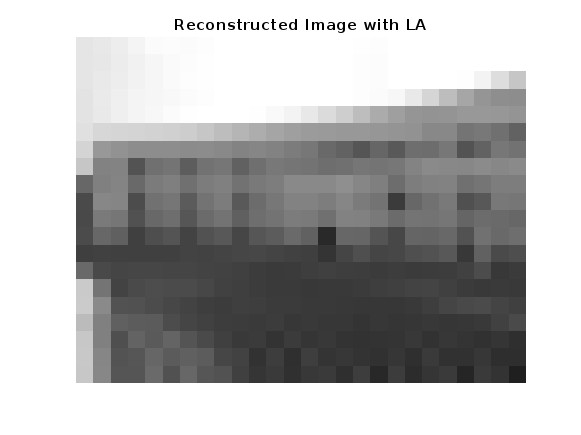
\includegraphics{gitsRC.jpg}

Before proceeding further just compare the size of its' original clean
image and the low-quality image shown in Figure

\begin{Shaded}
\begin{Highlighting}[]
\VariableTok{Original} \VariableTok{image} \VariableTok{size}\OperatorTok{:} \FloatTok{985.69} \VariableTok{KB}
\VariableTok{Reconstructed} \VariableTok{image} \VariableTok{size}\OperatorTok{:} \FloatTok{1.12} \VariableTok{KB}
\end{Highlighting}
\end{Shaded}

The reconstructed image is just 0.2\% of the original in size! This is
the core principle of optimizing image storage of CCTV system. This
resizing can be done and execute with optimal scaling with the help of
Linear Algebra. This module mainly focuses on such engineering
applications.

\section{Introduction}\label{introduction-2}

Spectral decomposition, also known as eigenvalue decomposition, is a
powerful tool in computational linear algebra that breaks down a matrix
into its eigenvalues and eigenvectors. This technique allows matrices to
be represented in terms of their fundamental components, making it
easier to analyze and manipulate them. It is especially useful for
symmetric matrices, which are common in various applications. Spectral
decomposition facilitates solving systems of equations, optimizing
functions, and performing transformations in a simplified, structured
manner, as it allows operations to be performed on the eigenvalues,
which often leads to more efficient computations.

The importance of spectral decomposition extends across a wide range of
fields, including computer science, engineering, and data science. In
machine learning, for instance, it forms the backbone of algorithms like
Principal Component Analysis (PCA), which is used for dimensionality
reduction. It also plays a vital role in numerical stability when
dealing with large matrices and is central to many optimization
problems, such as those found in machine learning and physics. Spectral
decomposition not only provides a deeper understanding of the properties
of matrices but also offers practical benefits in improving the
efficiency and accuracy of numerical algorithms.

\section{Spectral Decomposition: Detailed
Concepts}\label{spectral-decomposition-detailed-concepts}

\subsection{Eigenvalues and
Eigenvectors}\label{eigenvalues-and-eigenvectors}

The core idea behind spectral decomposition is that it expresses a
matrix in terms of its eigenvalues and eigenvectors. For a square matrix
\(A \in \mathbb{R}^{n \times n}\), an eigenvalue
\(\lambda \in \mathbb{R}\) and an eigenvector \(v \in \mathbb{R}^{n}\)
satisfy the following equation:

\[
A v = \lambda v
\]

This implies that when the matrix \(A\) acts on the vector \(v\), it
only scales the vector by \(\lambda\), but does not change its
direction. The eigenvector \(v\) represents the direction of this
scaling, while the eigenvalue \(\lambda\) represents the magnitude of
the scaling.

\begin{tcolorbox}[enhanced jigsaw, leftrule=.75mm, bottomtitle=1mm, colback=white, toptitle=1mm, opacitybacktitle=0.6, toprule=.15mm, colbacktitle=quarto-callout-note-color!10!white, arc=.35mm, colframe=quarto-callout-note-color-frame, title=\textcolor{quarto-callout-note-color}{\faInfo}\hspace{0.5em}{Properties of Eigen values}, titlerule=0mm, rightrule=.15mm, left=2mm, bottomrule=.15mm, breakable, coltitle=black, opacityback=0]

\begin{itemize}
\item
  If \(\lambda\) is an eigenvalue of \(A\), then it satisfies the
  characteristic polynomial:

  \[
  p(\lambda) = \text{det}(A - \lambda I) = 0.
  \]
\item
  The sum of the eigenvalues (counted with algebraic multiplicity) is
  equal to the trace of the matrix:

  \[
  \sum_{i=1}^{n} \lambda_i = \text{trace}(A).
  \]
\item
  The product of the eigenvalues (counted with algebraic multiplicity)
  is equal to the determinant of the matrix:

  \[
  \prod_{i=1}^{n} \lambda_i = \text{det}(A).
  \]
\item
  If\(A\) is symmetric, then:

  \begin{itemize}
  \tightlist
  \item
    All eigenvalues \(\lambda\) are real.
  \item
    If \(\lambda_i\) and \(\lambda_j\) are distinct eigenvalues, then
    their corresponding eigenvectors \(\mathbf{v}_i\) and
    \(\mathbf{v}_j\) satisfy:
  \end{itemize}

  \[
  \mathbf{v}_i^T \mathbf{v}_j = 0.
  \]
\item
  If \(A\) is a scalar multiple of \(k\), then:

  \[
  \lambda_i \text{ of } kA = k \cdot \lambda_i \text{ of } A.
  \]
\item
  If \(A\) is invertible, then:

  \[
  \lambda_i \text{ of } A^{-1} = \frac{1}{\lambda_i \text{ of } A}.
  \]
\item
  If \(A\) and \(B\) are similar, then:

  \[
  B = P^{-1} A P \implies \lambda_i \text{ of } B = \lambda_i \text{ of } A.
  \]
\item
  If \(\lambda\) is an eigenvalue, it has:

  \begin{itemize}
  \tightlist
  \item
    \textbf{Algebraic Multiplicity}: The number of times \(\lambda\)
    appears as a root of \(p(\lambda)\).
  \item
    \textbf{Geometric Multiplicity}: The dimension of the eigenspace
    \(E_{\lambda} = \{\mathbf{v} : A\mathbf{v} = \lambda \mathbf{v}\}\).
  \end{itemize}
\item
  If\(A\) is symmetric and all eigenvalues \(\lambda\) are positive,
  then \(A\) is positive definite:

  \[
  \lambda_i > 0 \implies A \text{ is positive definite.}
  \]
\item
  A square matrix \(A\) has an eigenvalue \(\lambda = 0\) if and only if
  \(A\) is singular:

  \[
  \text{det}(A) = 0 \iff \lambda = 0.
  \]
\end{itemize}

\end{tcolorbox}

\begin{tcolorbox}[enhanced jigsaw, leftrule=.75mm, bottomtitle=1mm, colback=white, toptitle=1mm, opacitybacktitle=0.6, toprule=.15mm, colbacktitle=quarto-callout-important-color!10!white, arc=.35mm, colframe=quarto-callout-important-color-frame, title=\textcolor{quarto-callout-important-color}{\faExclamation}\hspace{0.5em}{Eigen Vectors}, titlerule=0mm, rightrule=.15mm, left=2mm, bottomrule=.15mm, breakable, coltitle=black, opacityback=0]

Eigen vectors are the non-trivial solutions of \(det(A-\lambda I)=0\)
for distinct \(\lambda\).

\end{tcolorbox}

\begin{tcolorbox}[enhanced jigsaw, leftrule=.75mm, bottomtitle=1mm, colback=white, toptitle=1mm, opacitybacktitle=0.6, toprule=.15mm, colbacktitle=quarto-callout-note-color!10!white, arc=.35mm, colframe=quarto-callout-note-color-frame, title=\textcolor{quarto-callout-note-color}{\faInfo}\hspace{0.5em}{Properties of Eigen vectors}, titlerule=0mm, rightrule=.15mm, left=2mm, bottomrule=.15mm, breakable, coltitle=black, opacityback=0]

\begin{itemize}
\item
  If \(\mathbf{v}\) is an eigenvector of a square matrix \(A\)
  corresponding to the eigenvalue \(\lambda\), then:

  \[
  A\mathbf{v} = \lambda \mathbf{v}.
  \]
\item
  Eigenvectors corresponding to distinct eigenvalues are linearly
  independent. If \(\lambda_1\) and \(\lambda_2\) are distinct
  eigenvalues of \(A\), with corresponding eigenvectors \(\mathbf{v}_1\)
  and \(\mathbf{v}_2\), then:

  \[
  c_1 \mathbf{v}_1 + c_2 \mathbf{v}_2 = \mathbf{0} \implies c_1 = 0 \text{ and } c_2 = 0.
  \]
\item
  If \(\mathbf{v}\) is an eigenvector corresponding to the eigenvalue
  \(\lambda\), then any non-zero scalar multiple of \(\mathbf{v}\) is
  also an eigenvector corresponding to \(\lambda\):

  \[
  \text{If } \mathbf{v} \text{ is an eigenvector, then } c\mathbf{v} \text{ is an eigenvector for any non-zero scalar } c.
  \]
\item
  The eigenspace \(E_{\lambda}\) associated with an eigenvalue
  \(\lambda\) is defined as:

  \[
  E_{\lambda} = \{ \mathbf{v} : A\mathbf{v} = \lambda \mathbf{v} \} = \text{Null}(A - \lambda I).
  \]
\item
  The dimension of the eigenspace \(E_{\lambda}\) is equal to the
  geometric multiplicity of the eigenvalue \(\lambda\).
\item
  If \(A\) is a symmetric matrix, then eigenvectors corresponding to
  distinct eigenvalues are orthogonal:

  \[
  \mathbf{v}_i^T \mathbf{v}_j = 0 \text{ for distinct eigenvalues } \lambda_i \text{ and } \lambda_j.
  \]
\item
  For any square matrix \(A\), if \(\lambda = 0\) is an eigenvalue, the
  eigenvectors corresponding to this eigenvalue form the null space of
  \(A\):

  \[
  E_{0} = \{ \mathbf{v} : A\mathbf{v} = \mathbf{0} \} = \text{Null}(A).
  \]
\item
  If\(A\) is invertible, then \(A\) has no eigenvalue equal to zero,
  meaning all eigenvectors correspond to non-zero eigenvalues.
\item
  For\(A\) as a scalar multiple of \(k\):

  \[
  A\mathbf{v} = k \lambda \mathbf{v} \text{ for eigenvalue } \lambda.
  \]
\end{itemize}

\end{tcolorbox}

\subsection{Eigenvalue Decomposition (Spectral
Decomposition)}\label{eigenvalue-decomposition-spectral-decomposition}

For matrices that are diagonalizable (including symmetric matrices),
spectral decomposition expresses the matrix as a combination of its
eigenvalues and eigenvectors. Specifically, for a matrix \(A\), spectral
decomposition is represented as:

\[
A = V \Lambda V^{-1}
\]

where: - \(V\) is the matrix of eigenvectors of \(A\), - \(\Lambda\) is
a diagonal matrix of eigenvalues of \(A\), - \(V^{-1}\) is the inverse
of the matrix of eigenvectors (if \(V\) is invertible).

For symmetric matrices \(A\), the decomposition becomes simpler:

\[
A = Q \Lambda Q^\top
\]

Here, \(Q\) is an orthogonal matrix of eigenvectors (i.e.,
\(Q^\top Q = I\)), and \(\Lambda\) is a diagonal matrix of eigenvalues.

\subsection{Geometric Interpretation}\label{geometric-interpretation}

Eigenvalues and eigenvectors provide insights into the geometry of
linear transformations represented by matrices. Eigenvectors represent
directions that remain invariant under the transformation, while
eigenvalues indicate how these directions are stretched or compressed.

For example, in the case of a transformation matrix that scales or
rotates data points, eigenvalues show the magnitude of scaling along the
principal axes (directions defined by eigenvectors).

\subsection{Importance of
Diagonalization}\label{importance-of-diagonalization}

The key advantage of spectral decomposition is that it simplifies matrix
operations. When a matrix is diagonalized as \(A = Q \Lambda Q^\top\),
any function of the matrix \(A\) (such as powers, exponentials, or
inverses) can be easily computed by operating on the diagonal matrix
\(\Lambda\). For example:

\[
A^k = Q \Lambda^k Q^\top
\]

Since \(\Lambda\) is diagonal, raising \(\Lambda\) to any power \(k\) is
straightforward, involving only raising each eigenvalue to the power
\(k\).

\subsection{Properties of Symmetric
Matrices}\label{properties-of-symmetric-matrices}

Spectral decomposition applies particularly well to symmetric matrices,
which satisfy \(A = A^\top\). Symmetric matrices have the following key
properties:

\begin{itemize}
\item
  \textbf{Real eigenvalues}: The eigenvalues of a symmetric matrix are
  always real numbers.
\item
  \textbf{Orthogonal eigenvectors}: The eigenvectors corresponding to
  distinct eigenvalues of a symmetric matrix are orthogonal to each
  other.
\item
  \textbf{Diagonalizability}: Every symmetric matrix can be diagonalized
  by an orthogonal matrix.
\end{itemize}

These properties make symmetric matrices highly desirable in
computational applications.

\section{Mathematical Requirements for Spectral
Decomposition}\label{mathematical-requirements-for-spectral-decomposition}

\subsection{Determining Eigenvalues and
Eigenvectors}\label{determining-eigenvalues-and-eigenvectors}

The eigenvalues of a matrix \(A\) are the solutions to the
characteristic equation:

\[
\text{det}(A - \lambda I) = 0
\]

Here, \(I\) is the identity matrix, and \(\lambda\) represents the
eigenvalues. Solving this polynomial equation provides the eigenvalues
\(\lambda_1, \lambda_2, \dots, \lambda_n\). Once the eigenvalues are
determined, the eigenvectors can be computed by solving the equation
\((A - \lambda I)v = 0\) for each eigenvalue.

\subsection{\texorpdfstring{Characteristic Polynomial of \(2 \times 2\)
Matrices}{Characteristic Polynomial of 2 \textbackslash times 2 Matrices}}\label{characteristic-polynomial-of-2-times-2-matrices}

For a \(2 \times 2\) matrix: \[
A = \begin{pmatrix} a & b \\ c & d \end{pmatrix}
\] the characteristic polynomial is derived from the determinant of
\(A - \lambda I\), where \(I\) is the identity matrix:

\[
\det(A - \lambda I) = 0
\]

This leads to: \[
\det\begin{pmatrix} a - \lambda & b \\ c & d - \lambda \end{pmatrix} = (a - \lambda)(d - \lambda) - bc = 0
\]

\textbf{Short-cut Method:} The characteristic polynomial can be
simplified to: \[
\lambda^2 - (a + d)\lambda + (ad - bc) = 0
\]

This polynomial can be solved using the quadratic formula: \[
\lambda = \frac{(a + d) \pm \sqrt{(a + d)^2 - 4(ad - bc)}}{2}
\]

\begin{tcolorbox}[enhanced jigsaw, leftrule=.75mm, bottomtitle=1mm, colback=white, toptitle=1mm, opacitybacktitle=0.6, toprule=.15mm, colbacktitle=quarto-callout-important-color!10!white, arc=.35mm, colframe=quarto-callout-important-color-frame, title=\textcolor{quarto-callout-important-color}{\faExclamation}\hspace{0.5em}{Shortcut to write Characteristic polynomial of a \(2\times 2\) matrix}, titlerule=0mm, rightrule=.15mm, left=2mm, bottomrule=.15mm, breakable, coltitle=black, opacityback=0]

If \(A=\begin{bmatrix} a & b\\ c& d\end{bmatrix}\), then the
characteristic polynomial is
\[\lambda^2-(\text{Trace}(A))\lambda+det(A)=0\]

Eigen vectors can be found by using the formula: \begin{equation*}
EV(\lambda=\lambda_1)=\begin{bmatrix}\lambda_1-d\\ c\end{bmatrix}
\end{equation*}

\end{tcolorbox}

\subsection{Problems}\label{problems}

\textbf{Example 1:} Find Eigenvalues and Eigenvectors of the matrix,
\[A = \begin{pmatrix} 3 & 2 \\ 4 & 1 \end{pmatrix}\]

\emph{Solution:}

The characteristic equation is given by \[det(A-\lambda I)=0\]

\begin{align*}
\lambda^2 - 4\lambda - 5 &= 0\\
(\lambda-5)(\lambda+1)&=0\\
\end{align*}

Hence the eigen values are \(\lambda_1=5,\quad \lambda_2=-1\).

So the eigen vectors are: \begin{align*}
EV(\lambda=\lambda_1)&=\begin{bmatrix}\lambda_1-d\\ c\end{bmatrix}\\
\therefore EV(\lambda=5)&=\begin{bmatrix}4\\ 4\end{bmatrix}=\begin{bmatrix}1\\ 1\end{bmatrix}\\
\therefore EV(\lambda=-1)&=\begin{bmatrix}-2\\ 4\end{bmatrix}=\begin{bmatrix}-1\\ 2\end{bmatrix}
\end{align*}

\textbf{Problem 2:} Calculate the eigenvalues and eigenvectors of the
matrix: \(A = \begin{pmatrix} 2 & 1 \\ 1 & 2 \end{pmatrix}\)

\emph{Solution:}

To find the eigenvalues and eigenvectors of a \(2 \times 2\) matrix, we
can use the shortcut formula for the characteristic polynomial:

\[
\lambda^2 - \text{trace}(A)\lambda + \det(A) = 0,
\]

where \(A\) is the matrix. Let's apply this to the matrix

\[
A = \begin{pmatrix} 2 & 1 \\ 1 & 2 \end{pmatrix}.
\]

First, we calculate the trace and determinant of \(A\):

\begin{itemize}
\tightlist
\item
  The trace is the sum of the diagonal elements:
\end{itemize}

\[
\text{trace}(A) = 2 + 2 = 4.
\]

\begin{itemize}
\tightlist
\item
  The determinant is calculated as follows:
\end{itemize}

\[
\det(A) = (2)(2) - (1)(1) = 4 - 1 = 3.
\]

Next, substituting the trace and determinant into the characteristic
polynomial gives:

\[
\lambda^2 - (4)\lambda + 3 = 0,
\]

which simplifies to:

\[
\lambda^2 - 4\lambda + 3 = 0.
\]

We can factor this quadratic equation:

\[
(\lambda - 1)(\lambda - 3) = 0.
\]

Setting each factor to zero gives the eigenvalues:

\[
\lambda_1 = 1, \quad \lambda_2 = 3.
\]

To find the eigenvectors corresponding to each eigenvalue, we use the
shortcut for the eigenvector of a \(2 \times 2\) matrix
\(A = \begin{pmatrix} a & b \\ c & d \end{pmatrix}\):

\[
EV(\lambda) = \begin{pmatrix} \lambda - d \\ c \end{pmatrix}.
\]

For the eigenvalue \(\lambda_1 = 1\):

\[
EV(1) = \begin{pmatrix} 1 - 2 \\ 1 \end{pmatrix} = \begin{pmatrix} -1 \\ 1 \end{pmatrix}.
\]

This eigenvector can be simplified (up to a scalar multiple) to:

\[
\mathbf{v_1} = \begin{pmatrix} 1 \\ -1 \end{pmatrix}.
\]

For the eigenvalue \(\lambda_2 = 3\):

\[
EV(3) = \begin{pmatrix} 3 - 2 \\ 1 \end{pmatrix} = \begin{pmatrix} 1 \\ 1 \end{pmatrix}.
\]

This eigenvector is already in a simple form:

\[
\mathbf{v_2} = \begin{pmatrix} 1 \\ 1 \end{pmatrix}.
\]

\textbf{Problem 3:} For the matrix:
\(A = \begin{pmatrix} 1 & 2 & 1 \\ 0 & 1 & 0 \\ 1 & 0 & 1 \end{pmatrix}\),
find the eigenvalues and eigenvectors.

\emph{Solution:}

We are given the matrix \[
A = \begin{pmatrix} 1 & 2 & 1 \\ 0 & 1 & 0 \\ 1 & 0 & 1 \end{pmatrix}
\]

and we aim to find its eigenvalues using the characteristic polynomial.

The shortcut formula for the characteristic polynomial of a
\(3 \times 3\) matrix is given by: \[
\lambda^3 - \text{tr}(A)\lambda^2 + (\text{sum of principal minors of } A)\lambda - \det(A) = 0.
\]

The trace of a matrix is the sum of its diagonal elements. For matrix
\(A\), we have: \[
\text{tr}(A) = 1 + 1 + 1 = 3.
\]

The principal minors are the determinants of the \(2 \times 2\)
submatrices obtained by deleting one row and one column of \(A\).

The first minor is obtained by deleting the third row and third column:
\[
\det\begin{pmatrix} 1 & 2 \\ 0 & 1 \end{pmatrix} = (1)(1) - (2)(0) = 1.
\]

The second minor is obtained by deleting the second row and second
column: \[
\det\begin{pmatrix} 1 & 1 \\ 1 & 1 \end{pmatrix} = (1)(1) - (1)(1) = 0.
\]

The third minor is obtained by deleting the first row and first column:
\[
\det\begin{pmatrix} 1 & 0 \\ 0 & 1 \end{pmatrix} = (1)(1) - (0)(0) = 1.
\]

Thus, the sum of the principal minors is: \[
1 + 0 + 1 = 2.
\]

The determinant of \(A\) can be calculated using cofactor expansion
along the first row: \[
\det(A) = 1 \cdot \det\begin{pmatrix} 1 & 0 \\ 0 & 1 \end{pmatrix} - 2 \cdot \det\begin{pmatrix} 0 & 0 \\ 1 & 1 \end{pmatrix} + 1 \cdot \det\begin{pmatrix} 0 & 1 \\ 1 & 0 \end{pmatrix}
\] \[
= 1 \cdot (1) - 2 \cdot (0) + 1 \cdot (-1) = 1 - 0 - 1 = 0.
\]

Now, we substitute these values into the characteristic polynomial
formula: \[
\lambda^3 - \text{tr}(A)\lambda^2 + (\text{sum of principal minors})\lambda - \det(A) = 0
\] \[
\lambda^3 - 3\lambda^2 + 2\lambda - 0 = 0.
\]

We now solve the equation: \[
\lambda^3 - 3\lambda^2 + 2\lambda = 0.
\] Factoring out \(\lambda\) and apply factor theorem, we get:

\begin{align*}
   \lambda(\lambda^2 - 3\lambda + 2) &= 0\\
   \lambda(\lambda-2)(\lambda-1)&=0
\end{align*}

This gives one eigenvalue: \[
\lambda_1 = 0;\quad \lambda_2=2;\quad \lambda_3=1
\]

Now we find the eigenvectors corresponding to each eigenvalue.

For \(\lambda_1 = 0\), solve \((A - 0I)\mathbf{v} = 0\): \[
\begin{pmatrix} 1 & 2 & 1 \\ 0 & 1 & 0 \\ 1 & 0 & 1 \end{pmatrix} \begin{pmatrix} x \\ y \\ z \end{pmatrix} = \begin{pmatrix} 0 \\ 0 \\ 0 \end{pmatrix}.
\] This gives the system: \[
x + 2y + z = 0, \quad y = 0, \quad x + z = 0.
\] Thus, \(x = -z\), and the eigenvector is: \[
\mathbf{v}_1 = \begin{pmatrix} -1 \\ 0 \\ 1 \end{pmatrix}.
\]

For \(\lambda_2 = 2\), solve \((A - 2I)\mathbf{v} = 0\): \[
\begin{pmatrix} -1 & 2 & 1 \\ 0 & -1 & 0 \\ 1 & 0 & -1 \end{pmatrix} \begin{pmatrix} x \\ y \\ z \end{pmatrix} = \begin{pmatrix} 0 \\ 0 \\ 0 \end{pmatrix}.
\] This gives the system: \[
-x + 2y + z = 0, \quad -y = 0, \quad x - z = 0.
\] Thus, \(x = z\), and the eigenvector is: \[
\mathbf{v}_2 = \begin{pmatrix} 1 \\ 0 \\ 1 \end{pmatrix}.
\]

For \(\lambda_3 = 1\), solve \((A - I)\mathbf{v} = 0\): \[
\begin{pmatrix} 0 & 2 & 1 \\ 0 & 0 & 0 \\ 1 & 0 & 0 \end{pmatrix} \begin{pmatrix} x \\ y \\ z \end{pmatrix} = \begin{pmatrix} 0 \\ 0 \\ 0 \end{pmatrix}.
\] This gives the system: \[
2y + z = 0, \quad x = 0.
\] Thus, \(z = -2y\), and the eigenvector is: \[
\mathbf{v}_3 = \begin{pmatrix} 0 \\ 1 \\ -2 \end{pmatrix}.
\]

\textbf{Problem 3:} If
\(A=\begin{bmatrix}1&2&4\\ 0&3&4\\ 1&-1&-1 \end{bmatrix}\), compute the
eigen values and eigen vectors and left eigen vectors of \(A\).

\emph{Solution:}

We are given the matrix \[
A = \begin{pmatrix} 1 & 2 & 4 \\ 0 & 3 & 4 \\ 1 & -1 & -1 \end{pmatrix}
\]

and need to find its eigenvalues and eigenvectors.

The characteristic polynomial for a \(3 \times 3\) matrix is given by:
\[
\lambda^3 - \text{tr}(A)\lambda^2 + (\text{sum of principal minors})\lambda - \det(A) = 0.
\]

The trace is the sum of the diagonal elements: \[
\text{tr}(A) = 1 + 3 + (-1) = 3.
\]

We now compute the \(2 \times 2\) principal minors:

\begin{itemize}
\item
  Minor by removing the third row and third column: \[
  \det\begin{pmatrix} 1 & 2 \\ 0 & 3 \end{pmatrix} = (1)(3) - (2)(0) = 3.
  \]
\item
  Minor by removing the second row and second column: \[
  \det\begin{pmatrix} 1 & 4 \\ 1 & -1 \end{pmatrix} = (1)(-1) - (4)(1) = -1 - 4 = -5.
  \]
\item
  Minor by removing the first row and first column: \[
  \det\begin{pmatrix} 3 & 4 \\ -1 & -1 \end{pmatrix} = (3)(-1) - (4)(-1) = -3 + 4 = 1.
  \]
\end{itemize}

Thus, the sum of the principal minors is: \[
3 + (-5) + 1 = -1.
\]

We calculate the determinant of \(A\) by cofactor expansion along the
first row: \[
\det(A) = 1 \cdot \det\begin{pmatrix} 3 & 4 \\ -1 & -1 \end{pmatrix} - 2 \cdot \det\begin{pmatrix} 0 & 4 \\ 1 & -1 \end{pmatrix} + 4 \cdot \det\begin{pmatrix} 0 & 3 \\ 1 & -1 \end{pmatrix}.
\] The \(2 \times 2\) determinants are: \[
\det\begin{pmatrix} 3 & 4 \\ -1 & -1 \end{pmatrix} = -3 + 4 = 1, \quad \det\begin{pmatrix} 0 & 4 \\ 1 & -1 \end{pmatrix} = -4,
\] \[
\det\begin{pmatrix} 0 & 3 \\ 1 & -1 \end{pmatrix} = -3.
\]

Thus: \[
\det(A) = 1 \cdot 1 - 2 \cdot (-4) + 4 \cdot (-3) = 1 + 8 - 12 = -3.
\]

Substituting into the characteristic polynomial: \[
\lambda^3 - \text{tr}(A)\lambda^2 + (\text{sum of principal minors})\lambda - \det(A) = 0,
\]

we get: \[
\lambda^3 - 3\lambda^2 - \lambda + 3 = 0.
\]

We now solve the cubic equation: \begin{align*}
   \lambda^3 - 3\lambda^2 - \lambda + 3& = 0. \\
   (\lambda-1)(\lambda+1)(\lambda -3)&=0
\end{align*}

\[\lambda_1 = 1, \quad \lambda_2 = -1, \quad \lambda_3 = 3.\]

To find the eigenvector corresponding to \(\lambda_1 = 3\), solve
\((A - 3I)\mathbf{v} = 0\): \[
A - 3I = \begin{pmatrix} 1 & 2 & 4 \\ 0 & 3 & 4 \\ 1 & -1 & -1 \end{pmatrix} - 3\begin{pmatrix} 1 & 0 & 0 \\ 0 & 1 & 0 \\ 0 & 0 & 1 \end{pmatrix} = \begin{pmatrix} -2 & 2 & 4 \\ 0 & 0 & 4 \\ 1 & -1 & -4 \end{pmatrix}.
\]

Solving this system gives the eigenvector: \[
\mathbf{v}_1 = \begin{pmatrix} 1 \\ 1 \\ 0 \end{pmatrix}.
\]

For \(\lambda_2 = -1\), solve \((A +I)\mathbf{v} = 0\): \[
A +I = \begin{pmatrix} 1 & 2 & 4 \\ 0 & 3 & 4 \\ 1 & -1 & -1 \end{pmatrix} +\begin{pmatrix} 1 & 0 & 0 \\ 0 & 1 & 0 \\ 0 & 0 & 1 \end{pmatrix} = \begin{pmatrix} 2 & 2 & 4 \\ 0 & 4 & 4 \\ 1 & -1 & 0 \end{pmatrix}.
\]

Note that the third row is depending on first and second rows. So by
finding the cross product of first two rows,

\[
\mathbf{v}_2 = \begin{pmatrix} -1 \\ -1 \\ 1 \end{pmatrix}.
\]

For \(\lambda_3 = 1\), solve \((A -I)\mathbf{v} = 0\): \[
A - I = \begin{pmatrix} 1 & 2 & 4 \\ 0 & 3 & 4 \\ 1 & -1 & -1 \end{pmatrix} -\begin{pmatrix} 1 & 0 & 0 \\ 0 & 1 & 0 \\ 0 & 0 & 1 \end{pmatrix} = \begin{pmatrix} 0 & 2 & 4 \\ 0 & 2 & 4 \\ 1 & -1 & -2\end{pmatrix}.
\]

Note that the second row is same as first row. So by finding the cross
product of first and third rows, \[
\mathbf{v}_3 = \begin{pmatrix} 0 \\ -2 \\ 1 \end{pmatrix}.
\]

Thus, the eigenvalues of the matrix are: \[
\lambda_1 = 3, \quad \lambda_2 = -1, \quad \lambda_3 = 1
\]

with corresponding eigenvectors
\(\mathbf{v}_1=\begin{pmatrix} 1 \\ 1 \\ 0 \end{pmatrix}\),
\(\mathbf{v}_2=\begin{pmatrix} -1 \\ -1 \\ 1 \end{pmatrix}\), and
\(\mathbf{v}_3=\begin{pmatrix} 0 \\ -2 \\ 1 \end{pmatrix}\).

Left eigen vectors of the matrix \(A\) are eigen vectors of \(A^T\).

Here \(A^T=\begin{bmatrix}
    1&0&1\\ 2&3&-1\\ 4&4&-1
\end{bmatrix}\).

Since \(A\) and \(A^T\) have same eigen values, it is enough to find
corresponding eigen vectors. When \(\lambda=3\), the coefficient matrix
of \((A-\lambda I)X=0\) reduced into \(\begin{bmatrix}
    -2&0&1\\ 2&0&-1\\ 4&4&-4
\end{bmatrix}\)

Here the only independent rows are first and last. So the eigen vector
can be found as the cross product of these two rows.
\(\therefore v_1=\begin{bmatrix}
    1\\1\\2
\end{bmatrix}\).

When \(\lambda=-1\), the coefficient matrix of \((A-\lambda I)X=0\)
reduced into \(\begin{bmatrix}
    2&0&1\\ 2&4&-1\\ 4&4&0
\end{bmatrix}\)

Here the only independent rows are first and second. So the eigen vector
can be found as the cross product of these two rows.
\(\therefore v_2=\begin{bmatrix}
    -1\\1\\2
\end{bmatrix}\). When \(\lambda=1\), the coefficient matrix of
\((A-\lambda I)X=0\) reduced into \(\begin{bmatrix}
    0&0&1\\ 2&2&-1\\ 4&4&-2
\end{bmatrix}\)

Here the only independent rows are first and second. So the eigen vector
can be found as the cross product of these two rows.
\(\therefore v_2=\begin{bmatrix}
    -1\\1\\0
\end{bmatrix}\).

\subsection{\texorpdfstring{\texttt{Python} code to find eigen values
and eigen
vectors}{Python code to find eigen values and eigen vectors}}\label{python-code-to-find-eigen-values-and-eigen-vectors}

\begin{enumerate}
\def\labelenumi{\arabic{enumi}.}
\tightlist
\item
  Find eigen values and eigen vectors of
  \(A=\begin{bmatrix} 2&1\\ 1&2\end{bmatrix}\).
\end{enumerate}

\begin{Shaded}
\begin{Highlighting}[]
\ImportTok{import}\NormalTok{ numpy }\ImportTok{as}\NormalTok{ np}
\ImportTok{from}\NormalTok{ scipy.linalg }\ImportTok{import}\NormalTok{ null\_space}

\CommentTok{\# Define matrix A}
\NormalTok{A }\OperatorTok{=}\NormalTok{ np.array([[}\DecValTok{2}\NormalTok{, }\DecValTok{1}\NormalTok{], }
\NormalTok{              [}\DecValTok{1}\NormalTok{, }\DecValTok{2}\NormalTok{]])}

\CommentTok{\# Find eigenvalues}
\NormalTok{eigenvalues, \_ }\OperatorTok{=}\NormalTok{ np.linalg.eig(A)}

\CommentTok{\# Define identity matrix I}
\NormalTok{I }\OperatorTok{=}\NormalTok{ np.eye(A.shape[}\DecValTok{0}\NormalTok{])}

\CommentTok{\# Iterate over eigenvalues to find corresponding eigenvectors}
\ControlFlowTok{for}\NormalTok{ i, eigenvalue }\KeywordTok{in} \BuiltInTok{enumerate}\NormalTok{(eigenvalues):}
    \CommentTok{\# Compute A {-} lambda * I}
\NormalTok{    A\_lambda\_I }\OperatorTok{=}\NormalTok{ A }\OperatorTok{{-}}\NormalTok{ eigenvalue }\OperatorTok{*}\NormalTok{ I}
    
    \CommentTok{\# Find the null space (which gives the eigenvector)}
\NormalTok{    eig\_vector }\OperatorTok{=}\NormalTok{ null\_space(A\_lambda\_I)}
    
    \BuiltInTok{print}\NormalTok{(}\SpecialStringTok{f"Eigenvalue }\SpecialCharTok{\{}\NormalTok{i}\OperatorTok{+}\DecValTok{1}\SpecialCharTok{\}}\SpecialStringTok{: }\SpecialCharTok{\{}\NormalTok{eigenvalue}\SpecialCharTok{\}}\SpecialStringTok{"}\NormalTok{)}
    \BuiltInTok{print}\NormalTok{(}\SpecialStringTok{f"Eigenvector }\SpecialCharTok{\{}\NormalTok{i}\OperatorTok{+}\DecValTok{1}\SpecialCharTok{\}}\SpecialStringTok{:}\CharTok{\textbackslash{}n}\SpecialCharTok{\{}\NormalTok{eig\_vector}\SpecialCharTok{\}}\CharTok{\textbackslash{}n}\SpecialStringTok{"}\NormalTok{)}
\end{Highlighting}
\end{Shaded}

\begin{verbatim}
Eigenvalue 1: 3.0
Eigenvector 1:
[[0.70710678]
 [0.70710678]]

Eigenvalue 2: 1.0
Eigenvector 2:
[[-0.70710678]
 [ 0.70710678]]
\end{verbatim}

Same can be done using direct approach. Code for this task is given
below.

\begin{Shaded}
\begin{Highlighting}[]
\ImportTok{import}\NormalTok{ numpy }\ImportTok{as}\NormalTok{ np}

\CommentTok{\# Define matrix A}
\NormalTok{A }\OperatorTok{=}\NormalTok{ np.array([[}\DecValTok{2}\NormalTok{, }\DecValTok{1}\NormalTok{], }
\NormalTok{              [}\DecValTok{1}\NormalTok{, }\DecValTok{2}\NormalTok{]])}

\CommentTok{\# Find eigenvalues and eigenvectors}
\NormalTok{eigenvalues, eigenvectors }\OperatorTok{=}\NormalTok{ np.linalg.eig(A)}

\CommentTok{\# Display the results}
\BuiltInTok{print}\NormalTok{(}\StringTok{"Eigenvalues:"}\NormalTok{, eigenvalues)}
\BuiltInTok{print}\NormalTok{(}\StringTok{"Eigenvectors:}\CharTok{\textbackslash{}n}\StringTok{"}\NormalTok{, eigenvectors)}
\end{Highlighting}
\end{Shaded}

\begin{verbatim}
Eigenvalues: [3. 1.]
Eigenvectors:
 [[ 0.70710678 -0.70710678]
 [ 0.70710678  0.70710678]]
\end{verbatim}

\subsection{Diagonalization of Symmetric
Matrices}\label{diagonalization-of-symmetric-matrices}

For a symmetric matrix \(A\), the process of diagonalization can be
summarized as follows:

\begin{enumerate}
\def\labelenumi{\arabic{enumi}.}
\item
  \textbf{Compute eigenvalues}: Solve the characteristic equation
  \(\text{det}(A - \lambda I) = 0\) to find the eigenvalues.
\item
  \textbf{Find eigenvectors}: For each eigenvalue \(\lambda_i\), solve
  \((A - \lambda_i I)v_i = 0\) to find the corresponding eigenvector
  \(v_i\).
\item
  \textbf{Form the eigenvector matrix}: Arrange the eigenvectors into a
  matrix \(Q\), with each eigenvector as a column.
\item
  \textbf{Form the diagonal matrix of eigenvalues}: Construct
  \(\Lambda\) by placing the eigenvalues along the diagonal of the
  matrix.
\end{enumerate}

Thus, the matrix can be expressed as \(A = Q \Lambda Q^\top\).

\begin{enumerate}
\def\labelenumi{\arabic{enumi}.}
\tightlist
\item
  Diagonalize the matrix \(A=\begin{bmatrix} 2&1\\ 1&2\end{pmatrix}\).
\end{enumerate}

\texttt{Python} code for this task is given below.

\begin{Shaded}
\begin{Highlighting}[]
\ImportTok{import}\NormalTok{ numpy }\ImportTok{as}\NormalTok{ np}

\CommentTok{\# Define matrix A}
\NormalTok{A }\OperatorTok{=}\NormalTok{ np.array([[}\DecValTok{2}\NormalTok{, }\DecValTok{1}\NormalTok{], }
\NormalTok{              [}\DecValTok{1}\NormalTok{, }\DecValTok{2}\NormalTok{]])}

\CommentTok{\# Step 1: Find eigenvalues and eigenvectors}
\NormalTok{eigenvalues, eigenvectors }\OperatorTok{=}\NormalTok{ np.linalg.eig(A)}

\CommentTok{\# Step 2: Construct the diagonal matrix D (eigenvalues)}
\NormalTok{D }\OperatorTok{=}\NormalTok{ np.diag(eigenvalues)}

\CommentTok{\# Step 3: Construct the matrix P (eigenvectors)}
\NormalTok{P }\OperatorTok{=}\NormalTok{ eigenvectors}

\CommentTok{\# Step 4: Calculate the inverse of P}
\NormalTok{P\_inv }\OperatorTok{=}\NormalTok{ np.linalg.inv(P)}

\CommentTok{\# Verify the diagonalization: A = P D P\_inv}
\NormalTok{A\_reconstructed }\OperatorTok{=}\NormalTok{ P }\OperatorTok{@}\NormalTok{ D }\OperatorTok{@}\NormalTok{ P\_inv}

\BuiltInTok{print}\NormalTok{(}\StringTok{"Matrix A:"}\NormalTok{)}
\BuiltInTok{print}\NormalTok{(A)}

\BuiltInTok{print}\NormalTok{(}\StringTok{"}\CharTok{\textbackslash{}n}\StringTok{Eigenvalues (Diagonal matrix D):"}\NormalTok{)}
\BuiltInTok{print}\NormalTok{(D)}

\BuiltInTok{print}\NormalTok{(}\StringTok{"}\CharTok{\textbackslash{}n}\StringTok{Eigenvectors (Matrix P):"}\NormalTok{)}
\BuiltInTok{print}\NormalTok{(P)}

\BuiltInTok{print}\NormalTok{(}\StringTok{"}\CharTok{\textbackslash{}n}\StringTok{Inverse of P:"}\NormalTok{)}
\BuiltInTok{print}\NormalTok{(P\_inv)}

\BuiltInTok{print}\NormalTok{(}\StringTok{"}\CharTok{\textbackslash{}n}\StringTok{Reconstructed matrix A (P D P\^{}({-}1)):"}\NormalTok{)}
\BuiltInTok{print}\NormalTok{(A\_reconstructed)}
\end{Highlighting}
\end{Shaded}

\begin{verbatim}
Matrix A:
[[2 1]
 [1 2]]

Eigenvalues (Diagonal matrix D):
[[3. 0.]
 [0. 1.]]

Eigenvectors (Matrix P):
[[ 0.70710678 -0.70710678]
 [ 0.70710678  0.70710678]]

Inverse of P:
[[ 0.70710678  0.70710678]
 [-0.70710678  0.70710678]]

Reconstructed matrix A (P D P^(-1)):
[[2. 1.]
 [1. 2.]]
\end{verbatim}

\subsection{Matrix Functions and Spectral
Theorem}\label{matrix-functions-and-spectral-theorem}

Once a matrix is diagonalized, various matrix functions become easier to
compute. For a function \(f(A)\), such as the exponential of a matrix or
any power, the function can be applied to the diagonal matrix of
eigenvalues:

\[
f(A) = Q f(\Lambda) Q^\top
\]

where \(f(\Lambda)\) is the function applied element-wise to the
eigenvalues in the diagonal matrix \(\Lambda\).

\subsection{Symmetric Positive Definite
Matrices}\label{symmetric-positive-definite-matrices}

A special class of matrices, symmetric positive definite matrices, are
often used in optimization and machine learning. These matrices have all
positive eigenvalues, ensuring that the matrix is invertible and has a
unique decomposition.

\section{Computational Aspects}\label{computational-aspects}

Spectral decomposition is computationally intensive, particularly for
large matrices. Efficient numerical algorithms like the \textbf{QR
algorithm} and \textbf{Jacobi method} are used to compute eigenvalues
and eigenvectors in practice. For dense matrices, algorithms scale as
\(O(n^3)\), but specialized methods exist for sparse matrices that take
advantage of matrix structure to reduce computational cost.

\section{Practical Applications}\label{practical-applications}

\begin{itemize}
\tightlist
\item
  \textbf{Principal Component Analysis (PCA)}: Used to reduce the
  dimensionality of datasets by finding the principal components
  (eigenvectors) that capture the most variance in the data.
\item
  \textbf{Quantum Mechanics}: Eigenvalue problems frequently arise in
  solving Schrödinger's equation, where eigenfunctions correspond to
  states of a quantum system, and eigenvalues represent observable
  quantities like energy.
\item
  \textbf{Markov Chains}: In probability and stochastic processes,
  spectral decomposition helps analyze long-term behavior by breaking
  down the transition matrix into eigenvalue components.
\item
  \textbf{Graph Theory}: The adjacency matrix of a graph can be
  decomposed using spectral methods to reveal properties like community
  structure and connectivity.
\end{itemize}

\section{Conclusion}\label{conclusion}

Spectral decomposition offers an elegant and practical framework for
understanding the fundamental structure of matrices. By reducing
matrices to their eigenvalues and eigenvectors, it simplifies numerous
computational tasks in linear algebra, making it an indispensable tool
in various applications such as machine learning, physics, and
optimization.

\bookmarksetup{startatroot}

\chapter*{References}\label{references}
\addcontentsline{toc}{chapter}{References}

\markboth{References}{References}

\phantomsection\label{refs}
\begin{CSLReferences}{1}{0}
\bibitem[\citeproctext]{ref-harris2020array}
Harris, Charles R., K. Jarrod Millman, Stéfan J. van der Walt, Ralf
Gommers, Pauli Virtanen, David Cournapeau, Eric Wieser, et al. 2020.
{``Array Programming with {NumPy}.''} \emph{Nature} 585 (7825): 357--62.
\url{https://doi.org/10.1038/s41586-020-2649-2}.

\bibitem[\citeproctext]{ref-strang2020linear}
Strang, Gilbert. 2020. \emph{Linear Algebra for Everyone}. SIAM.

\end{CSLReferences}




\end{document}
